% !Mode:: "TeX:UTF-8"
%这样可以确保 .tex 文件默认使用 UTF-8 的格式打开

%学位论文怎么写,这位教授说的太好了!
%https://mp.weixin.qq.com/s/NbPkZWytwiu-nBysj4P9HQ

\def\usewhat{pdflatex}                              % 定义编译方式 dvipdfmx 或者 pdflatex ,默认为 dvipdfmx
                                                    % 方式编译,如果需要修改,只需改变花括号中的内容即可。
%\setlength{\baselineskip}{20pt}
%\setlength{\headheight}{25pt}
\documentclass[a4paper,12.5pt,openany,twoside]{book}
%openright, openany 指定新的一章\chapter 是在奇数页(右侧)开头,还是直接紧跟着上 一页开头。report 缺省为openany,book 缺省为openright。【对article 无效】


                                           % 如果论文超过60页 可以使用twoside 双面打印
% !Mode:: "TeX:UTF-8"
%  Authors: franz tao  : franztaoheng@gmail.com     湖南大学2015级计算机科学与技术专业硕士生

%%%%%%%%%% Package %%%%%%%%%%%%
\usepackage{array}
\newcommand{\PreserveBackslash}[1]{\let\temp=\\#1\let\\=\temp}
\newcolumntype{C}[1]{>{\PreserveBackslash\centering}p{#1}}
\newcolumntype{R}[1]{>{\PreserveBackslash\raggedleft}p{#1}}
\newcolumntype{L}[1]{>{\PreserveBackslash\raggedright}p{#1}}

\usepackage[section]{algorithm}
\usepackage{algorithmic}
\renewcommand{\algorithmicrequire}{\textbf{Input:}}
\renewcommand{\algorithmicensure}{\textbf{Output:}}
\renewcommand{\algorithmiccomment}[1]{\hfill /* #1 */}



\usepackage{graphicx}                       % 支持插图处理
\usepackage{geometry}
\geometry{left=2.5cm,right=2.5cm,top=2cm,bottom=2.5cm,footskip=1.1cm,headsep=0.7cm,head=0.4cm}
                                            % 支持版面尺寸设置
\usepackage{titlesec}                       % 控制标题的宏包
\usepackage{titletoc}                       % 控制目录的宏包
\usepackage{fancyhdr}                       % fancyhdr宏包 支持页眉和页脚的相关定义
\usepackage[UTF8]{ctex}                     % 支持中文显示
\usepackage{color}                          % 支持彩色
\usepackage{amsmath}                        % AMSLaTeX宏包 用来排出更加漂亮的公式
\usepackage{amssymb}                        % 数学符号生成命令
\usepackage[below]{placeins}                %允许上一个section的浮动图形出现在下一个section的开始部分,还提供\FloatBarrier命令,使所有未处理的浮动图形立即被处理
\usepackage{flafter}                        % 使得所有浮动体不能被放置在其浮动环境之前,以免浮动体在引述它的文本之前出现.
\usepackage{multirow}                       % 使用Multirow宏包,使得表格可以合并多个row格
\usepackage{booktabs}                       % 表格,横的粗线;\specialrule{1pt}{0pt}{0pt}
\usepackage{longtable}                      % 支持跨页的表格。
\usepackage{tabularx}                       % 自动设置表格的列宽
\usepackage{setspace}
\usepackage{subfigure}                      % 支持子图 %centerlast 设置最后一行是否居中
\usepackage[subfigure]{ccaption}            % 支持子图的中文标题
\usepackage[sort&compress,numbers]{natbib}  % 支持引用缩写的宏包
\usepackage{enumitem}                       % 使用enumitem宏包,改变列表项的格式
\usepackage{calc}                           % 长度可以用+ - * / 进行计算
\usepackage{txfonts}                        % 字体宏包
\usepackage{bm}                             % 处理数学公式中的黑斜体的宏包
\usepackage[amsmath,thmmarks,hyperref]{ntheorem}  % 定理类环境宏包,其中 amsmath 选项用来兼容 AMS LaTeX 的宏包
\usepackage{CJKnumb}                        % 提供将阿拉伯数字转换成中文数字的命令
\usepackage{indentfirst}                    % 首行缩进宏包
\usepackage{CJKutf8}                        % 用在UTF8编码环境下,它可以自动调用CJK,同时针对UTF8编码作了设置。
\usepackage{CJK}
\usepackage{fancyhdr}
\usepackage{lastpage}
\usepackage{layout}
\usepackage[titles,subfigure]{tocloft}                       %控制生成的表格和图片的目录格式


\usepackage{tabularx}
\usepackage{epstopdf}

%\usepackage{hypbmsec}                      % 用来控制书签中标题显示内容

%如果您的pdf制作中文书签有乱码使用如下命令,就可以解决了
\usepackage[unicode,               % pdflatex, pdftex 这里决定运行文件的方式不同
            pdfstartview=FitH,
            %CJKbookmarks=true,
            bookmarksnumbered=true,
            bookmarksopen=true,
            colorlinks=true,
            pdfborder={0 0 1},
            citecolor=black,
            linkcolor=black,
            anchorcolor=black,
            urlcolor=black,
            breaklinks=true
            ]{hyperref}


                      % 定义本文所使用宏包
\graphicspath{{figures/}}                  % 定义所有的.eps文件在figures子目录下
\begin{document}                           % 开始全文
\begin{CJK*}{UTF8}{song}                   % 开始中文字体使用
% !Mode:: "TeX:UTF-8"
%  Authors: franz tao  : franztaoheng@gmail.com     湖南大学2015级计算机科学与技术专业硕士生

%%%%%%%%%% Fonts Definition and Basics %%%%%%%%%%%%%%%%%
\newcommand{\song}{\CJKfamily{song}}    % 宋体
\newcommand{\fs}{\CJKfamily{fs}}        % 仿宋体
\newcommand{\kai}{\CJKfamily{kai}}      % 楷体
\newcommand{\hei}{\CJKfamily{hei}}      % 黑体
\newcommand{\li}{\CJKfamily{li}}        % 隶书
\newcommand{\yihao}{\fontsize{26pt}{26pt}\selectfont}       % 一号, 1.倍行距
\newcommand{\xiaoyi}{\fontsize{24pt}{24pt}\selectfont}      % 小一, 1.倍行距
\newcommand{\erhao}{\fontsize{22pt}{22pt}\selectfont}       % 二号, 1.倍行距
\newcommand{\xiaoer}{\fontsize{18pt}{18pt}\selectfont}      % 小二, 单倍行距
\newcommand{\sanhao}{\fontsize{16pt}{16pt}\selectfont}      % 三号, 1.倍行距
\newcommand{\xiaosan}{\fontsize{15pt}{15pt}\selectfont}     % 小三, 1.倍行距
\newcommand{\sihao}{\fontsize{14pt}{14pt}\selectfont}       % 四号, 1.0倍行距
\newcommand{\xiaosi}{\fontsize{12.5pt}{12.5pt}\selectfont}      % 小四, 1. 倍行距
\newcommand{\wuhao}{\fontsize{10.5pt}{10.5pt}\selectfont}   % 五号, 单倍行距
\newcommand{\xiaowu}{\fontsize{9pt}{9pt}\selectfont}        % 小五, 单倍行距
\setlength{\headheight}{20pt}
%\CJKcaption{gb_452}
\CJKtilde  % 重新定义了波浪符~的意义
\newcommand\prechaptername{第}
\newcommand\postchaptername{章}

% 调整罗列环境的布局
\setitemize{leftmargin=3em,itemsep=0em,partopsep=0em,parsep=0em,topsep=-0em}
\setenumerate{leftmargin=3em,itemsep=0em,partopsep=0em,parsep=0em,topsep=0em}


%避免宏包 hyperref 和 arydshln 不兼容带来的目录链接失效的问题。
\def\temp{\relax}
\let\temp\addcontentsline
\gdef\addcontentsline{\phantomsection\temp}

% 自定义项目列表标签及格式 \begin{publist} 列表项 \end{publist}
\newcounter{pubctr} %自定义新计数器
\newenvironment{publist}{%%%%%定义新环境
\begin{list}{[\arabic{pubctr}]} %%标签格式
    {
     \usecounter{pubctr}
     \setlength{\leftmargin}{2em}     % 左边界 \leftmargin =\itemindent + \labelwidth + \labelsep
     \setlength{\itemindent}{0em}     % 标号缩进量
     \setlength{\labelsep}{1em}       % 标号和列表项之间的距离,默认0.5em
     \setlength{\rightmargin}{0em}    % 右边界
     \setlength{\topsep}{0ex}         % 列表到上下文的垂直距离
     \setlength{\parsep}{0ex}         % 段落间距
     \setlength{\itemsep}{0ex}        % 标签间距
     \setlength{\listparindent}{0pt} % 段落缩进量
    }}
{\end{list}}%%%%%


\makeatletter
\renewcommand\normalsize{
  \@setfontsize\normalsize{12.5pt}{12.5pt} % 小四对应12pt
  \setlength\abovedisplayskip{4pt}
  \setlength\abovedisplayshortskip{4pt}
  \setlength\belowdisplayskip{\abovedisplayskip}
  \setlength\belowdisplayshortskip{\abovedisplayshortskip}
    \let\@listi\@listI}
\def\defaultfont{\renewcommand{\baselinestretch}{1.65}\normalsize\selectfont}


% 设置行距和段落间垂直距离

\setlength{\baselineskip}{20pt}
\renewcommand{\CJKglue}{\hskip 0.5pt plus \baselineskip} %加大字间距,使每行35个字


\makeatother

%%%%%%%%%%%%% Contents %%%%%%%%%%%%%%%%%
\renewcommand{\contentsname}{目\qquad 录}
\setcounter{tocdepth}{2}
\titlecontents{chapter}[0em]{\xiaosi\hei}%
             {\prechaptername~~\thecontentslabel~~\postchaptername~~~}{} %
             {\titlerule*[5pt]{$\cdot$}\xiaosi\contentspage}
\titlecontents{section}[2em]{\xiaosi\song} %
            {\thecontentslabel\quad}{} %
            {\hspace{.25em}\titlerule*[5pt]{$\cdot$}\xiaosi\contentspage}
\titlecontents{subsection}[4em]{\xiaosi\song} %
            {\thecontentslabel\quad}{} %
            {\hspace{.25em}\titlerule*[5pt]{$\cdot$}\xiaosi\contentspage}
\renewcommand{\cftdotsep}{1.1}
\renewcommand{\listfigurename}{插图索引}
\setcounter{lofdepth}{1}
%\titlefigures{chapter}[1em]{\xiaosi\hei}%
             %{\prechaptername~~\thecontentslabel~~\postchaptername~~~}{} %
            % {\titlerule*[10pt]{$\cdot$}\xiaosi\contentspage}
\renewcommand{\listtablename}{附表索引}


%%删除表格和插图因章不同中的空行%%%
\makeatletter
\def\@chapter[#1]#2{\ifnum \c@secnumdepth >\m@ne
                       \if@mainmatter
                         \refstepcounter{chapter}%
                         \typeout{\@chapapp\space\thechapter.}%
                         \addcontentsline{toc}{chapter}%
                                   {\protect\numberline{\thechapter}#1}%
                       \else
                         \addcontentsline{toc}{chapter}{#1}%
                       \fi
                    \else
                      \addcontentsline{toc}{chapter}{#1}%
                    \fi
                    \chaptermark{#1}%
                    \if@twocolumn
                      \@topnewpage[\@makechapterhead{#2}]%
                    \else
                      \@makechapterhead{#2}%
                      \@afterheading
                    \fi}
\makeatother


%%%%%%%%%% Chapter and Section %%%%%%%%%%%%%%%%%
\setcounter{secnumdepth}{4}
\setlength{\parindent}{2em}
\renewcommand{\chaptername}{\prechaptername\arabic{chapter}\postchaptername}
\titleformat{\chapter}{\centering\xiaoer\hei}{\chaptername}{1em}{}
\titlespacing{\chapter}{0pt}{0pt}{18pt}
\titleformat{\section}{\xiaosan\hei}{\thesection}{1em}{}
\titlespacing{\section}{0pt}{12pt}{12pt}
\titleformat{\subsection}{\sihao\hei}{\thesubsection}{0.5em}{}
\titlespacing{\subsection}{0pt}{6pt}{6pt}
\titleformat{\subsubsection}{\xiaosi\hei}{\thesubsubsection}{0.5em}{}
\titlespacing{\subsubsection}{0pt}{6pt}{6pt}

%%%%%%%%%% Table, Figure and Equation %%%%%%%%%%%%%%%%%
\renewcommand{\tablename}{表} % 插表题头
\renewcommand{\figurename}{图} % 插图题头
\renewcommand{\thefigure}{\arabic{chapter}.\arabic{figure}} % 使图编号为 7.1 的格式 %\protect{~}
\renewcommand{\thetable}{\arabic{chapter}.\arabic{table}}%使表编号为 7.1 的格式
\renewcommand{\theequation}{\arabic{chapter}.\arabic{equation}}%使公式编号为 7-1 的格式
\renewcommand{\thesubfigure}{(\alph{subfigure})}%使子图编号为 (a)的格式
\renewcommand{\thesubtable}{(\alph{subtable})} %使子表编号为 (a)的格式
\makeatletter
\renewcommand{\p@subfigure}{\thefigure~} %使子图引用为 7-1 a) 的格式,母图编号和子图编号之间用~加一个空格
\makeatother


%% 定制浮动图形和表格标题样式
\makeatletter
\long\def\@makecaption#1#2{%
   \vskip\abovecaptionskip
   \sbox\@tempboxa{\centering\wuhao\hei{#1~~#2} }%
   \ifdim \wd\@tempboxa >\hsize
     \centering\wuhao\hei{#1~~#2} \par
   \else
     \global \@minipagefalse
     \hb@xt@\hsize{\hfil\box\@tempboxa\hfil}%
   \fi
   \vskip\belowcaptionskip}
\makeatother
\captiondelim{~~~~} %用来控制longtable表头分隔符

%%%%%%%%%% Theorem Environment %%%%%%%%%%%%%%%%%
\theoremstyle{plain}
\theorembodyfont{\song\rmfamily}
\theoremheaderfont{\hei\rmfamily}
\newtheorem{theorem}{定理~}[chapter]
\newtheorem{lemma}{引理~}[chapter]
\newtheorem{axiom}{公理~}[chapter]
\newtheorem{proposition}{命题~}[chapter]
\newtheorem{corollary}{推论~}[chapter]
\newtheorem{definition}{定义~}[chapter]
\newtheorem{conjecture}{猜想~}[chapter]
\newtheorem{example}{例~}[chapter]
\newtheorem{remark}{注~}[chapter]
\floatname{algorithm}{算法}%将英文的algorithm改为算法
\renewcommand{\algorithmicrequire}{\textbf{Input:}}
\renewcommand{\algorithmicensure}{\textbf{Output:}}
\newenvironment{proof}{\noindent{\hei 证明:}}{\hfill $ \square $ \vskip 4mm}
\theoremsymbol{$\square$}

\makeatletter
\@addtoreset{algorithm}{chapter}
\makeatother
%%%%%%%%%% Page: number, header and footer  页码%%%%%%%%%%%%%%%%%

%\frontmatter 或 \pagenumbering{roman}
%\mainmatter 或 \pagenumbering{arabic}
\makeatletter
\renewcommand\frontmatter{\clearpage
  \@mainmatterfalse
  \pagenumbering{Roman}} % 正文前罗马字体编号
\makeatother


%%%%%%%%%% References %%%%%%%%%%%%%%%%%
\renewcommand{\bibname}{参考文献}
% 重定义参考文献样式,来自thu
\makeatletter
\renewenvironment{thebibliography}[1]{%
   \chapter*{\bibname}%
   \xiaosi
   \list{\@biblabel{\@arabic\c@enumiv}}%
        {\renewcommand{\makelabel}[1]{##1\hfill}
         \setlength{\baselineskip}{21pt}
         \settowidth\labelwidth{0.5cm}
         \setlength{\labelsep}{0pt}
         \setlength{\itemindent}{0pt}
         \setlength{\leftmargin}{\labelwidth+\labelsep}
         \addtolength{\itemsep}{-0.7em}
         \usecounter{enumiv}%
         \let\p@enumiv\@empty
         \renewcommand\theenumiv{\@arabic\c@enumiv}}%
    \sloppy\frenchspacing
    \clubpenalty4000%
    \@clubpenalty \clubpenalty
    \widowpenalty4000%
    \interlinepenalty4000%
    \sfcode`\.\@m}
   {\def\@noitemerr
     {\@latex@warning{Empty `thebibliography' environment}}%
    \endlist\frenchspacing}
\makeatother

\addtolength{\bibsep}{5pt} % 增加参考文献间的垂直间距
\setlength{\bibhang}{2em} %每个条目自第二行起缩进的距离

% 参考文献引用作为上标出现
\newcommand{\mycite}[1]{\scalebox{1.3}[1.3]{\raisebox{-0.65ex}{\cite{#1}}}}

%% 引用格式
\bibpunct{[}{]}{,}{s}{}{,}

%%%%%%%%%% Cover %%%%%%%%%%%%%%%%%
% 封面、摘要、版权、致谢格式定义
\makeatletter

%\def\dtitle#1{\def\@dtitle{#1}}\def\@dtitle{}
\def\ctitle#1{\def\@ctitle{#1}}\def\@ctitle{}
\def\etitle#1{\def\@etitle{#1}}\def\@etitle{}
\def\caffil#1{\def\@caffil{#1}}\def\@caffil{}
\def\cmacrosubject#1{\def\@cmacrosubject{#1}}\def\@cmacrosubject{}
\def\cmacrosubjecttitle#1{\def\@cmacrosubjecttitle{#1}}\def\@cmacrosubjecttitle{}
\def\csubject#1{\def\@csubject{#1}}\def\@csubject{}
\def\csubjecttitle#1{\def\@csubjecttitle{#1}}\def\@csubjecttitle{}
\def\cmajor#1{\def\@cmajor{#1}}\def\@cmajor{}
\def\cauthor#1{\def\@cauthor{#1}}\def\@cauthor{}
\def\cauthortitle#1{\def\@cauthortitle{#1}}\def\@cauthortitle{}
\def\csupervisor#1{\def\@csupervisor{#1}}\def\@csupervisor{}
\def\csupervisortitle#1{\def\@csupervisortitle{#1}}\def\@csupervisortitle{}
\def\cdate#1{\def\@cdate{#1}}\def\@cdate{}
\def\untitle#1{\def\@untitle{#1}}\def\@untitle{}
\def\declaretitle#1{\def\@declaretitle{#1}}\def\@declaretitle{}
\def\declarecontent#1{\def\@declarecontent{#1}}\def\@declarecontent{}
\def\authorizationtitle#1{\def\@authorizationtitle{#1}}\def\@authorizationtitle{}
\def\authorizationcontent#1{\def\@authorizationcontent{#1}}\def\@authorizationconent{}
\def\authorizationadd#1{\def\@authorizationadd{#1}}\def\@authorizationadd{}
\def\authorsigncap#1{\def\@authorsigncap{#1}}\def\@authorsigncap{}
\def\supervisorsigncap#1{\def\@supervisorsigncap{#1}}\def\@supervisorsigncap{}
\def\signdatecap#1{\def\@signdatecap{#1}}\def\@signdatecap{}
\long\def\cabstract#1{\long\def\@cabstract{#1}}\long\def\@cabstract{}
\long\def\eabstract#1{\long\def\@eabstract{#1}}\long\def\@eabstract{}
\def\ckeywords#1{\def\@ckeywords{#1}}\def\@ckeywords{}
\def\ekeywords#1{\def\@ekeywords{#1}}\def\@ekeywords{}
\def\cheading#1{\def\@cheading{#1}}\def\@cheading{}
\def\cnumber#1{\def\@cnumber{#1}}\def\@cnumber{}
\def\csecret#1{\def\@csecret{#1}}\def\@csecret{}
\def\chnunumer#1{\def\@chnunumer{#1}}\def\@chnunumer{}
\def\cclassnumber#1{\def\@cclassnumber{#1}}\def\@cclassnumber{}
\def\chnuname#1{\def\@chnuname{#1}}\def\@chnuname{}
\def\cchair#1{\def\@cchair{#1}}\def\@cchair{}
\def\ddate#1{\def\@ddate{#1}}\def\@ddate{}
%英文内封
\def\ename#1{\def\@ename{#1}}\def\@ename{}
\def\cbe#1{\def\@cbe{#1}}\def\@cbe{}
\def\cms#1{\def\@cms{#1}}\def\@cms{}
\def\cdegree#1{\def\@cdegree{#1}}\def\@cdegree{}
\def\cclass#1{\def\@cclass{#1}}\def\@cclass{}
\def\emajor#1{\def\@emajor{#1}}\def\@emajor{}
\def\ehnu#1{\def\@ehnu{#1}}\def\@ehnu{}
\def\esupervisor#1{\def\@esupervisor{#1}}\def\@esupervisor{}
\def\edate#1{\def\@edate{#1}}\def\@edate{}
\def\elevel#1{\def\@elevel{#1}}\def\@elevel{}


\newlength{\@title@width}
\def\@put@covertitle#1{\makebox[\@title@width][s]{#1}}
% 定义封面
\def\makecover{
%\cleardoublepage%
   \phantomsection
    \pdfbookmark[-1]{\@ctitle}{ctitle}

    \begin{titlepage}
    \begin{center}

      \setlength{\@title@width}{3.5cm}
       {
  \begin{tabular}{lcclc}
   \xiaosi\hei{学校代号}&  \underline{\makebox[\@title@width][c]{\@chnunumer}}&\qquad \qquad \qquad \qquad \qquad & \xiaosi\hei{学\qquad 号}&  \underline{\makebox[\@title@width][c]{\@cnumber}}\\
   \xiaosi\hei{分~~类~~~号}&  \underline{\makebox[\@title@width][c]{\@cclassnumber}}&\qquad \qquad \qquad \qquad \qquad & \xiaosi\hei{密\qquad 级}&  \underline{\makebox[\@title@width][c]{\@csecret}} \\
   \end{tabular}
   }

 \begin{figure}[h]
  \centering
  
\includegraphics[width=0.3\textwidth]{figures/Hnulogo}
  \end{figure}
      \vspace*{1cm}
      {\hei\erhao \@cheading}

      \vspace*{1cm}


      \begin{center}
      \begin{spacing}{1.5}
      \hei\yihao \@ctitle
      \end{spacing}
      \end{center}

      \vspace{\baselineskip}
      \setlength{\@title@width}{6.5cm}
  {

  \begin{spacing}{2.1}
   \xiaosi\hei{学位申请人姓名} \xiaosi\song\underline{\makebox[\@title@width][l]{\qquad\@cauthor}} \\
   \xiaosi\hei{培~~~~养~~~~~单~~~~~位} \xiaosi\song\underline{\makebox[\@title@width][l]{\qquad\@caffil}} \\
   \xiaosi\hei{导师姓名及职称} \xiaosi\song\underline{\makebox[\@title@width][l]{\qquad\@csupervisor}} \\
   \xiaosi\hei{学~~~~科~~~~~专~~~~~业} \xiaosi\song\underline{\makebox[\@title@width][l]{\qquad\@csubject}} \\
   \xiaosi\hei{研~~~~究~~~~~方~~~~~向} \xiaosi\song\underline{\makebox[\@title@width][l]{\qquad\@cmajor}}\\
   \xiaosi\hei{论~文~提~交~日~~期} \xiaosi\song\underline{\makebox[\@title@width][l]{\qquad\@cdate}} \\
  %\end{tabular}
  \end{spacing}
 }
 \end{center}


\clearpage
\thispagestyle{empty} %去掉页眉页脚

\noindent
\makebox[2.59cm][s]{}{\begin{tabular}{ll}
\xiaosi\hei 学校代号:\xiaosi\song~~\@chnunumer \\
\xiaosi\hei 学\qquad~号:\xiaosi\song~~\@cnumber\\
\xiaosi\hei 密\qquad~级:\xiaosi\song~~\@csecret\\
\end{tabular}
}

%
\vspace{5\baselineskip}

\noindent
\makebox[2.59cm][s]{}{
\xiaoer\song \@chnuname \@cheading
}
\\
\vspace{4\baselineskip}

\begin{spacing}{2}
\hangafter=1\hangindent=2.7cm   %换行后自动缩进
{\noindent
\makebox[2.59cm][s]{} {\hei\erhao\@ctitle}}
\end{spacing}
\vspace{4\baselineskip}

\setlength{\@title@width}{6.8cm}
  {
  \begin{spacing}{2}
  \xiaosi
   \noindent
  \makebox[2.59cm][s]{}{
  \begin{tabular}{lc}
   \underline{\xiaosi\hei学位申请人姓名:\song\makebox[\@title@width][l]{\qquad\qquad\@cauthor}} \\
   \underline{\xiaosi\hei导师姓名及职称:\song\makebox[\@title@width][l]{\qquad\qquad\@csupervisor}} \\
   \underline{\xiaosi\hei培~~~~养~~~~~单~~~~位:\song\makebox[\@title@width][l]{\qquad\qquad\@caffil}} \\
   \underline{\xiaosi\hei专~~~~业~~~~~名~~~~称:\song\makebox[\@title@width][l]{\qquad\qquad\@csubject}} \\
   \underline{\xiaosi\hei论~文~提~交~日~期:\song\makebox[\@title@width][l]{\qquad\qquad\@cdate}} \\
   \underline{\xiaosi\hei论~文~答~辩~日~期:\song\makebox[\@title@width][l]{\qquad\qquad\@ddate}}\\
   \underline{\xiaosi\hei答辩委员会主席:\song\makebox[\@title@width][l]{\qquad\qquad\@cchair}} \\
  \end{tabular}
  %\end{tabular}
    }
   \end{spacing}
    }

\clearpage
\thispagestyle{empty} %去掉页眉页脚

\begin{center}
\qquad\\
 \begin{spacing}{2.5}
 \xiaosan \@etitle

 \end{spacing}



 \begin{spacing}{2}
 \xiaosi
 by\\
 \@ename \\
 \@cbe\\
% \@cms\\
 A~\@cdegree~submitted in partial satisfaction of the\\
 requirements for the degree of\\
 \@cclass\\
 in\\
\@emajor\\
in the\\
Graduate school\\
 of\\
 \@ehnu\\

 \vspace{2\baselineskip}

Supervisor\\
\@elevel~~ \@esupervisor\\
\@edate
\end{spacing}

\end{center}


\end{titlepage}

%  另起一页: 独创性声明和学位论文版权使用授权书

\pagestyle{fancy}
\fancyhf{}
\fancyfoot[C]{\song\xiaowu ~\thepage~}
\renewcommand{\headrulewidth}{0pt}

    \addcontentsline{toc}{chapter}{学位论文原创性声明和学位论文版权使用授权书}{
    \setcounter{page}{1}
    \qquad\\
    \begin{center}\hei\xiaoer{\@untitle}\end{center}\par
    \begin{center}\hei\xiaoer{\@declaretitle}\end{center}\par
    \song\defaultfont{\@declarecontent}\par
    \vspace*{1cm}
    {\song\xiaosi
    \@authorsigncap \makebox[2.5cm][s]{}
    \@signdatecap \makebox[2cm][s]{} 年 \makebox[1cm][s]{} 月 \makebox[1cm][s]{} 日
    }
    \vspace{0.6\baselineskip}
    \begin{center}\hei\xiaoer{\@authorizationtitle}\end{center}\par
    {
    \vspace{1.2\baselineskip}
    \song\defaultfont{\@authorizationcontent}
    \begin{tabular}{ll}
     \song\defaultfont\@authorizationadd\par&\\
    &1、保密\song\xiaoer{$\Box$}\song\xiaosi ,在\underline{\qquad}年解密后适用于本授权书\\
    &2、不保密\song\xiaoer{$\Box$}。\\
    &(请在以上相应方框内打"$\surd$") \\
    \end{tabular}
    }
    \vspace{2\baselineskip}

    {
    \song\xiaosi
      \@authorsigncap \makebox[3.5cm][s]{}  \@signdatecap \makebox[1.5cm][s]{} 年 \makebox[1cm][s]{} 月 \makebox[1cm][s]{} 日 \\
      \indent
      \@supervisorsigncap \makebox[3.5cm][s]{}  \@signdatecap \makebox[1.5cm][s]{} 年 \makebox[1cm][s]{} 月 \makebox[1cm][s]{} 日
    }
    }


%%%%%%%%%%%%%%%%%%%   Abstract and Keywords  %%%%%%%%%%%%%%%%%%%%%%%
\clearpage

\pagestyle{fancy}
  \fancyhf{}
\fancyhead[CO]{\song\xiaowu \@cheading}
\fancyhead[CE]{\song\xiaowu \@ctitle}
\fancyfoot[C]{\song\xiaowu ~\thepage~}
\makeatletter %双线页眉
\def\headrule{{\if@fancyplain\let\headrulewidth\plainheadrulewidth\fi%
\hrule\@height 1.0pt \@width\headwidth\vskip1pt %上面线为1pt粗
\hrule\@height 0.5pt\@width\headwidth  %下面0.5pt粗
\vskip-2\headrulewidth\vskip-1pt}      %两条线的距离1pt
\vspace{7mm} %双线与下面正文之间的垂直间距
}

\fancypagestyle{plain}{% 设置开章页页眉页脚风格
    \fancyhf{}%
\fancyhead[CO]{\song\xiaowu \@cheading}
\fancyhead[CE]{\song\xiaowu \@ctitle}
\fancyfoot[C]{\song\xiaowu ~\thepage~} %首页页脚格式
%双线页眉的设置
\makeatletter %双线页眉
\def\headrule{{\if@fancyplain\let\headrulewidth\plainheadrulewidth\fi%
\hrule\@height 1.0pt \@width\headwidth\vskip1pt %上面线为1pt粗
\hrule\@height 0.5pt\@width\headwidth  %下面0.5pt粗
\vskip-2\headrulewidth\vskip-1pt}      %两条线的距离1pt
\vspace{7mm} %双线与下面正文之间的垂直间距
}

}
\addcontentsline{toc}{chapter}{摘~要}
\chapter*{\centering\xiaoer\ 摘\qquad 要}
\song\defaultfont
\@cabstract
\vspace{\baselineskip}

%\hangafter=1\hangindent=52.3pt\noindent   %如果取消该行注释,关键词换行时将会自动缩进
\noindent
{\hei\xiaosi 关键词: \@ckeywords}

%%%%%%%%%%%%%%%%%%%   English Abstract  %%%%%%%%%%%%%%%%%%%%%%%%%%%%%%
\clearpage

\addcontentsline{toc}{chapter}{Abstract}
\chapter*{\centering\xiaoer \bf{Abstract}}
%\vspace{\baselineskip}
\@eabstract
\vspace{\baselineskip}

%\hangafter=1\hangindent=60pt\noindent  %如果取消该行注释,KEY WORDS换行时将会自动缩进
\noindent
{\xiaosi\bf{Key Words: \@ekeywords}}
}
\clearpage
\makeatother
                       % 完成对论文各个部分格式的设置
\frontmatter                               % 以下是论文导言部分,包括论文的封面,中英文摘要和中文目录
% !Mode:: "TeX:UTF-8"

\chnunumer{10532}
\chnuname{湖南大学}
\cclassnumber{TP391}
%\cnumber{**}
\cnumber{S151000891}
\csecret{普通}
\cmajor{计算机网络}
\cheading{硕士学位论文}      % 设置正文的页眉,以及自己的学位级别
\ctitle{SDN/NFV网络架构可生存性算法研究}  %封面用论文标题,自己可手动断行
\etitle{The Research on SDN/NFV Network Architecture Survivable Algorithm }
\caffil{信息科学与工程学院} %学院名称
\csubjecttitle{学科专业}
\csubject{计算机科学与技术}   %专业
\cauthortitle{研究生}     % 学位
\cauthor{陶恒}   %学生姓名
%\cauthor{**}   %学生姓名
\ename{Heng~~TAO}
%\ename{*~~*}
\cbe{B.E.~(Hunan University of Science and Technology)~2015}
%\cms{M.S.~(Hunan University)~2018}
\cdegree{thesis}
\cclass{Master of engineering}
\emajor{Computer Science and Technology}
\ehnu{Hunan~University}
%\esupervisor{**}
\esupervisor{Kun Xie}
\csupervisortitle{指导教师}
\csupervisor{谢鲲~教授} %导师姓名
%\csupervisor{**~教授} %导师姓名
\elevel{Professor} %导师职称
\cchair{邝继顺~教授}%邝继顺
%\cchair{**}
\ddate{~~~~2018年~~~5月~~~20日}
\edate{May,~2018}
\untitle{湖~~南~~大~~学}
\declaretitle{学位论文原创性声明}
\declarecontent{
本人郑重声明:所呈交的论文是本人在导师的指导下独立进行研究所取得的研究成果。除了文中特别加以标注引用的内容外,本论文不包含任何其他个人或集体已经发表或撰写的成果作品。对本文的研究做出重要贡献的个人和集体,均已在文中以明确方式标明。本人完全意识到本声明的法律后果由本人承担。
}
\authorizationtitle{学位论文版权使用授权书}
\authorizationcontent{
本学位论文作者完全了解学校有关保留、使用学位论文的规定,同意学校保留并向国家有关部门或机构送交论文的复印件和电子版,允许论文被查阅和借阅。本人授权湖南大学可以将本学位论文的全部或部分内容编入有关数据库进行检索,可以采用影印、缩印或扫描等复制手段保存和汇编本学位论文。
}
\authorizationadd{本学位论文属于}
\authorsigncap{作者签名:}
\supervisorsigncap{导师签名:}
\signdatecap{签字日期:}


%\cdate{\CJKdigits{\the\year} 年\CJKnumber{\the\month} 月 \CJKnumber{\the\day} 日}
% 如需改成二零一二年四月二十五日的格式,可以直接输入,即如下所示
% \cdate{二零一二年四月二十五日}
\cdate{~~~~2018年~~~5月~~~8日} % 此日期显示格式为阿拉伯数字 如2012 年4 月25 日
\cabstract{
现如今网络整体规模和网络功能类型的复杂度越来越大,新技术对网络性能需求不断提高,传统的网络架构己经无法满足按需调动、快速配置等需求,软件定义网络(SDN)的提出就是为了应对现有网络架构无法解决的问题和突破网络性能瓶颈的限制。利用网络功能虚拟化(NFV)技术将网络资源进行虚拟化,在很大程度上可以解决现有网络无法解决的问题和到达现有网络无法达到的网络性能需求。网络服务运行在实际的物理设备上,这将必然产生不可避免的网络故障,SDN/NFV新型的网络架构在网络的可生存性领域比传统网络架构更加高效的检测、处理和恢复网络故障。

光网络和Overlay网络中为了保证网络的可生存性,基于SDN的架构能高效实现不相交路径路由功能,快速的在源节点和目的节点之间寻找满足一定QoS约束的不相交路由。当主用路径出现故障时,将其承载的业务流转换到备用路径上,从而实现快速的业务恢复,因此快速不相交路径算法的研究如今具有很高的研究价值。网络虚拟化的过程中,如何为虚拟网络在底层物理网中找到满足约束条件且最优的嵌入,并且提供可生存性保护需求,来保证底层物理网资源失效情况下原本虚拟网络的业务正常运行,可生存性虚拟网络嵌入问题的研究已经是NFV研究中的重要邻域。
%SDN作为新型网络架构,网络虚拟化作为未来网络研究的重要领域,两者的结合具有很高的研究意义。传统分布式网络通过复杂的MPLS协议来实现对源节点和目的节点之间提供多条QoS路径,以提高网络的可生存性,这一做法已不能满足在网络连接出现故障时保持业务高效灵活迅速的提供可生存性保护需求。嵌入算法主要是考虑虚拟网络节点和链路向底层物理网络的映射,

本文结合当今研究热点,基于SDN/NFV网络架构下以可生存性算法作为课题的研究方向,主要研究了以下三个方面的内容:

研究网络可生存性技术,对网络故障失效环境进行了研究,并且探讨了已有各种情形的路径保护算法和不相交路径算法。

研究共享风险链路组不相交的约束条件,提出冲突边集合的概念,通过容量设置来获得冲突边集合,以冲突边集合来分而治之原问题,并行解决SRLG不相交路由问题,并且与己有算法进行理论分析和实验对比,结果表明我提出的算法优于现有其它算法。

%其次,研究SDN虚拟网络技术,对SDN网络虚拟化的环境进行了研究,并且探讨了虚拟网络向底层物理网进行映射时的不同嵌入算法和可生存性嵌入算法。

研究节点和链路映射以及可生存性需求之间的关系,在可生存性虚拟网络嵌入算法的设计中,考虑到节点带有特定功能约束条件,本文结合已有算法的不足,提出了星型分解动态规划节点映射的可生存性虚拟网络嵌入算法,并且与己有算法进行实验对比,实验结果表明我提出的算法优于现有其它算法。
}
%中文摘要应将学位论文的内容要点简短明了地表达出来,约500~800字左右(限一页),字体为宋体小四号。内容应包括工作目的、研究方法、成果和结论。要突出本论文的创新点,语言力求精炼。为了便于文献检索,应在本页下方另起一行注明论文的关键词(3-7个)。
\ckeywords{软件定义网络;~~网络功能虚拟化;~~不相交路径;~~虚拟网络嵌入;~~ 可生存性;~~风险共享链路组}
\eabstract{Nowadays, the complexity of the whole network scale and the network function type is more and more large, the new technology is increasing the demand for network performance, and the traditional network architecture has been unable to meet the needs of on-demand mobilization, rapid configuration, and so on. Software defined Network (SDN) is proposed to deal with the existing network architecture can not solve the problem and break through the network performance bottlenecks. Using network function virtualization (NFV) technology to virtualize network resources can to a large extent solve the problems that the existing network cannot solve and reach the network performance requirements that the existing network cannot achieve. Network services run on actual physical devices, which will inevitably lead to inevitable network failures. SDN / NFV new network architecture can detect, process and recover network failures more efficiently than traditional network architecture in the field of network survivability.

In order to ensure the survivability of optical network and Overlay network, the architecture based on SDN can efficiently realize disjoint path routing function, and find disjoint routing between source node and destination node quickly. When the main path fails, the traffic flow is converted to the standby path, so the fast disjoint path algorithm has a high research value. In the process of network virtualization, how to find the best embedding in the underlying physical network, and how to provide survivability protection for the virtual network. To ensure the normal operation of the original virtual network under the condition of the failure of the underlying physical network resources, the research of the survivability virtual network embedding problem has become an important neighborhood in the research of NFV.

In this paper, based on the research direction of survivability algorithm under the SDN/NFV network architecture, we mainly study the following three aspects:

In this paper, the survivability technology of network is studied, and the fault failure environment of network is studied, and the existing path protection algorithms and disjoint path algorithms are discussed.  

In this paper, the constraint conditions of disjoint shared risk link group are studied, and the concept of conflict edge set is proposed. The conflict edge set is obtained by capacity setting, the original problem of dividing and dominating the conflict edge set is obtained, and the SRLG disjoint routing problem is solved in parallel. The theoretical analysis and experimental results show that the proposed algorithm is superior to other existing algorithms.  

This paper studies the relationship between node, link mapping and survivability requirements. In the design of survivability virtual network embedding algorithm, considering that nodes have specific functional constraints, this paper combines the shortcomings of existing algorithms. A survivabal virtual network embedding algorithm based on star decomposition dynamic programming node mapping is proposed and compared with the existing algorithms. The experimental results show that the proposed algorithm is superior to other existing algorithms.

}
\ekeywords{Software Defined Network(SDN);~~Network Function Virtualization(NFV);~~Disjoint Path;~~ Virtual Network Embedding(VNE);~~Survivability;~~Shared Risk Link Group(SRLG)}
\makecover
\clearpage
                      % 封面

%%%%%%%%%%   目录   %%%%%%%%%%
\defaultfont
\addcontentsline{toc}{chapter}{目~~~~录}
\tableofcontents                           % 中文目录
\clearpage
\newcommand{\loflabel}{图~}
\renewcommand{\numberline}[1]{\song\xiaosi\loflabel~#1\hspace*{\baselineskip}}
\addcontentsline{toc}{chapter}{插图索引}
\listoffigures
\clearpage
\newcommand{\lotlabel}{表~}
\renewcommand{\numberline}[1]{\song\xiaosi\lotlabel~#1\hspace*{\baselineskip}}
\addcontentsline{toc}{chapter}{附表索引}
\listoftables
\clearpage{\pagestyle{empty}\cleardoublepage}
%%%%%%%%%% 正文部分内容  %%%%%%%%%%
\mainmatter\defaultfont\sloppy\raggedbottom

\setlength{\intextsep}{2pt}
\renewcommand{\ALC@linenosize}{\xiaosi}
\renewcommand\arraystretch{1.5}
\setlength{\abovecaptionskip}{2pt}
\setlength{\belowcaptionskip}{2pt}
\hfuzz=\maxdimen
\tolerance=10000
\hbadness=10000


\newcommand{\revtao}[1]{\textcolor{orange}{{#1}}}%revise the text with blue color, you can use this one.
%\newcommand{\revtao}[1]{\textcolor{black}{{#1}}}%revise the text with blue color, you can use this one.
%\newcommand{\del}[1]{\sout{#1}}  %revise the text
%\newcommand{\del}[1]{}
%\newcommand{\note}[1]{{\sffamily\itshape\bfseries\uline{#1}}}
\newcommand{\CSLI}{SRLG Conflicting Link Set}
\newcommand{\CI}{SCLS}
\newcommand{\TopoNum}{7}


\chapter{绪论}
\section{研究背景及意义}
\subsection{课题研究背景}
在传统的网络架构中,数据平面和控制平面没有分离,是集成在同一处的硬件系统上的。这使得新业务在引进时十分不便,一方面需要在路由交换、数据处理等业务之外进行相关处理工作,宁一方面还需要在网络技术、支撑软件与业务创建软件等软件相关方面进行相应地设计与研究。这样来,使得网络运营商需要增加成本来进行运营维护,也阻碍了客户要求的队业务作出迅速响应的请求,同时也妨碍了业务的创新。

传统网络的层次结构是互联网取得巨大成功的关键.但是随着网络规模的不断扩大,封闭的网络设备内置了过多的复杂协议,增加了运营商定制优化网络的难度,科研人员无法在真实环境中规模部署新协议.同时,互联网流量的快速增长(预计到2018 年,全球流量将达到1.6*1021 字节[1]),用户对流量的需求不断扩大,各种新型服务不断出现,增加了网络运维成本.换机下发统一标准规则,交换机仅需按照这些规则执行相应的动作即可.因此,SDN 技术能够有效降低设备负载,协助网络运营商更好地控制基础设施,降低整体运营成本,成为最具前途的网络技术之一.因此,SDN 被MIT列为“改变世界的十大创新技术之一”[5].SDN 相关技术研究迅速开展起来,成为近年来的研究热点.2013 年,SIGCOMM 会议收录了多篇相关文章,甚至将SDN 列为专题来研讨,带动了SDN 相关研究的蓬勃发展.

随着网络的快速发展,传统互联网出现了如传统网络配置复杂度高等诸多问题[6],这些问题说明网络架构需要革新,可编程网络的相关研究为SDN 的产生提供了可参考的理论依据[7].主动网络[8,9]允许数据包携带用户程序,并能够由网络设备自动执行.用户可以通过编程方式动态地配置网络,达到了方便管理网络的目的.然而由于需求低、协议兼容性差等问题,并未在工业界实际部署.4D 架构[10,11]将可编程的决策平面(即控制层)从数据平面分离,使控制平面逻辑中心化与自动化,其设计思想产生SDN 控制器的雏形[12].
借鉴计算机系统的抽象结构,未来的网络结构将存在转发抽象、分布状态抽象和配置抽象这3 类虚拟化概念[13].转发抽象剥离了传统交换机的控制功能,将控制功能交由控制层来完成,并在数据层和控制层之间提供了标准接口,确保交换机完成识别转发数据的任务.控制层需要将设备的分布状态抽象成全网视图,以便众多应用能够通过全网信息进行网络的统一配置.配置抽象进一步简化了网络模型,用户仅需通过控制层提供的应用接口对网络进行简单配置,就可自动完成沿路径转发设备的统一部署.因此,网络抽象思想解耦了路径依赖,成为数据控制分离且接口统一架构(即SDN)产生的决定因素.此外,众多标准化组织已经加入到SDN相关标准的制订当中.专门负责订制SDN接口标准的著名组织是开
放网络基金会(Open Networking Foundation,简称ONF)[14],该组织制订的OpenFlow 协议业已成为SDN 接口的主流标准,许多运营商和生产厂商根据该标准进行研发.互联网工程任务组(Internet Engineering Task Force,简称IETF) 的ForCES 工作组[15]、互联网研究专门工作组(Internet Research Task Force,简称IRTF)的SDNRG 研究组[16]以及国际电信联盟远程通信标准化组织(ITU Telecommunication Standardization Sector,简称ITU-T)的多个工作组[17]同样针对SDN 的新方法和新应用等展开研究.标准化组织的跟进,促使了SDN 市场的快速发展.据悉,SDN 市场已于2013 年达到约2 亿美元的产值,预计到2016 年将达到20 亿美元[18],市场需求确保SDN 有足够的发展空间.由此可见,SDN 具有广阔的发展前景和巨大的研究价值.

QoS 约束的链路故障多备份路径恢复算法


随着通信技术的快速发展,网络链路带宽得到不断扩充。目前全球至少有来自20 多个国家的53个运营商已经部署或正在考虑部署 400 GB/s 的骨
干网络[1]。高速骨干网链路即使短暂的故障也会造成
大量的数据包丢弃,严重影响通信质量。根据对ISP
的观察,骨干网链路一年内大约有30%的概率会出
现故障[2],表明链路故障是网络中较为普遍的现象。
因此,加快故障的恢复速度,降低故障造成的业务
丢弃已成为当前研究亟待解决的问题。
网络故障主要表现为链路故障,链路故障恢复
策略可分为主动式和被动式两种[3,4]。被动式策略在
网络故障后动态自适应地进行全网资源重分配,但
路由重新收敛花费较多的时间而不可接受。因此目
前故障快速恢复研究以主动式策略为主,通过提前
对网络进行资源规划和预留,使得故障时能迅速切
换,如基于多拓扑[5]和基于备份路径的故障恢复技
术。多拓扑技术需要配置多个拓扑子层,路由存储
消耗大;基于备份路径的故障恢复技术提供端到端
路径重路由,在全局范围内进行流量分配,易于基
于现有协议实现。因此,备份路径技术是当前故障
恢复领域研究的热点[6-11]。
故障恢复的本质在于维持故障链路承载流量的
传输,因此应从流量持续传输角度解决故障恢复问
题。大部分故障恢复工作集中在如何选择可靠备份
路径上,且一般利用单一备份路径进行故障恢复。
然而当流量超出备份路径可用带宽时,单一备份路
径无法满足故障恢复的要求。受到这一启发,文献
[8]将多路径技术引入到故障恢复中,采用多条备份
路径共同承担流量,减少了流量的丢弃。在此基础
上,文献[9]提出一种结合故障恢复与流量工程的网
络结构,在多路径故障恢复基础上进行流量工程优
化,其目的是进行负载均衡,且假设备份路径可用
带宽满足故障恢复需求。文献[10]考虑了不同故障状
况,通过将重路由流量分配给有跳数限制的多条备
份路径,在网络投入运行之前就设计好应对各种故
障场景的最低容量备份网络。文献[11]提出一种跨层
故障恢复模型,考虑了备份链路的可靠性,提升了
故障恢复成功率。然而,上述故障恢复算法大都以
最大化重路由为目标,未考虑恢复后的流量是否满
足用户的需求。但是经由备份路径的重路由流量即
使最终传输成功,由于时延超时、链路过载等原因,
也无法满足业务的服务质量需求(Quality of Service,
QoS),属于无效流量。虽然文献[12]提出了一种满
足QoS 约束的自适应调整的多路径路由,但未考虑
故障恢复问题。因此,目前已提出的大部分链路故
障恢复算法不能很好地确保业务的服务质量。
为此,本文针对QoS 约束下的链路故障恢复问
题进行研究,即在网络可用带宽和业务时延需求约
束下进行最大化重路由流量问题求解。首先基于多
备份路径策略建立概率关联故障模型和重路由流量
丢弃优化目标,并构建QoS 约束的故障多备份路径
恢复问题的数学优化模型。然后,设计QoS 约束的
链路故障多备份路径恢复算法(Multiple backup
Paths Recovery for link failure with QoS constrain
algorithm, MPR-QoS) 对此问题进行求解。
MPR-QoS 算法在构建单条备份路径时,利用改进
的QoS 约束的k 最短路径法进行拼接,并以最大化
减少重路由流量丢弃为目标,且分配给高优先级链
路更多的保护资源。此外还证明了算法的正确性并
对时间空间复杂度进行了分析。最后,在NS2 仿真
环境下从故障恢复率、重路由流量QoS 满足率、链
路过载率和算法运行时间等方面验证了本文算法的
优越性。


SDN作为新型网络架构,数据网络中心作为未来网络研究的重要领域,SDN在数据中心网络的应用具有研究意义。

本文结合实际情况,以基于SDN网络的多路径路由技术作为课题的研究方向,主要研究以三个方面内容。


\subsection{课题研究目的和意义}


\section{预备知识}
\subsection{图论}
网络通常表示为图$G(\mathbb{V},\mathbb{E})$,其中$\mathbb{V}$是$|\mathbb{V}|$个节点的集合(例如,节点表示路由)和$\mathbb{E}$是$|\mathbb{E}|$条链路的集合(例如,链路代表光纤线路或无线电信道)。链接可能带有延迟、长度或成本等属性。对于每条链路$e_i$,$w_{e_i}$表示链路的权重。路径$P$的权重表示为路径$P$中每条链路的权重之和$w_P=\sum\limits_{e_i\in \mathbb{P}}w_{e_i}$。

共享风险链接组(SRLG)是一组链路共享同一个组件,该组件的故障会导致所有链路的故障。一条链接可以属于多个共享风险链接组里。举个例子,在光网络的导管中\cite{bhandari1994optimal}可以放置多条光链路,如图.\ref{fig:Logic shift operation}所示,链路(1,2),(3,2)和(3,4)放置在一个导管中,同时链路(3,2)和(3,4)也共同放置在另一个导管中。如果某个导管被切断,相应导管的链路将失效。每个导管对应一个共享风险链接组。其它共享风险链接组的应用是交通网络的相关拥塞和电网的级联故障\cite{coudert2007shared}。


\begin{figure}[htbp]
\centering
\subfigure[Physical topology with conduit]{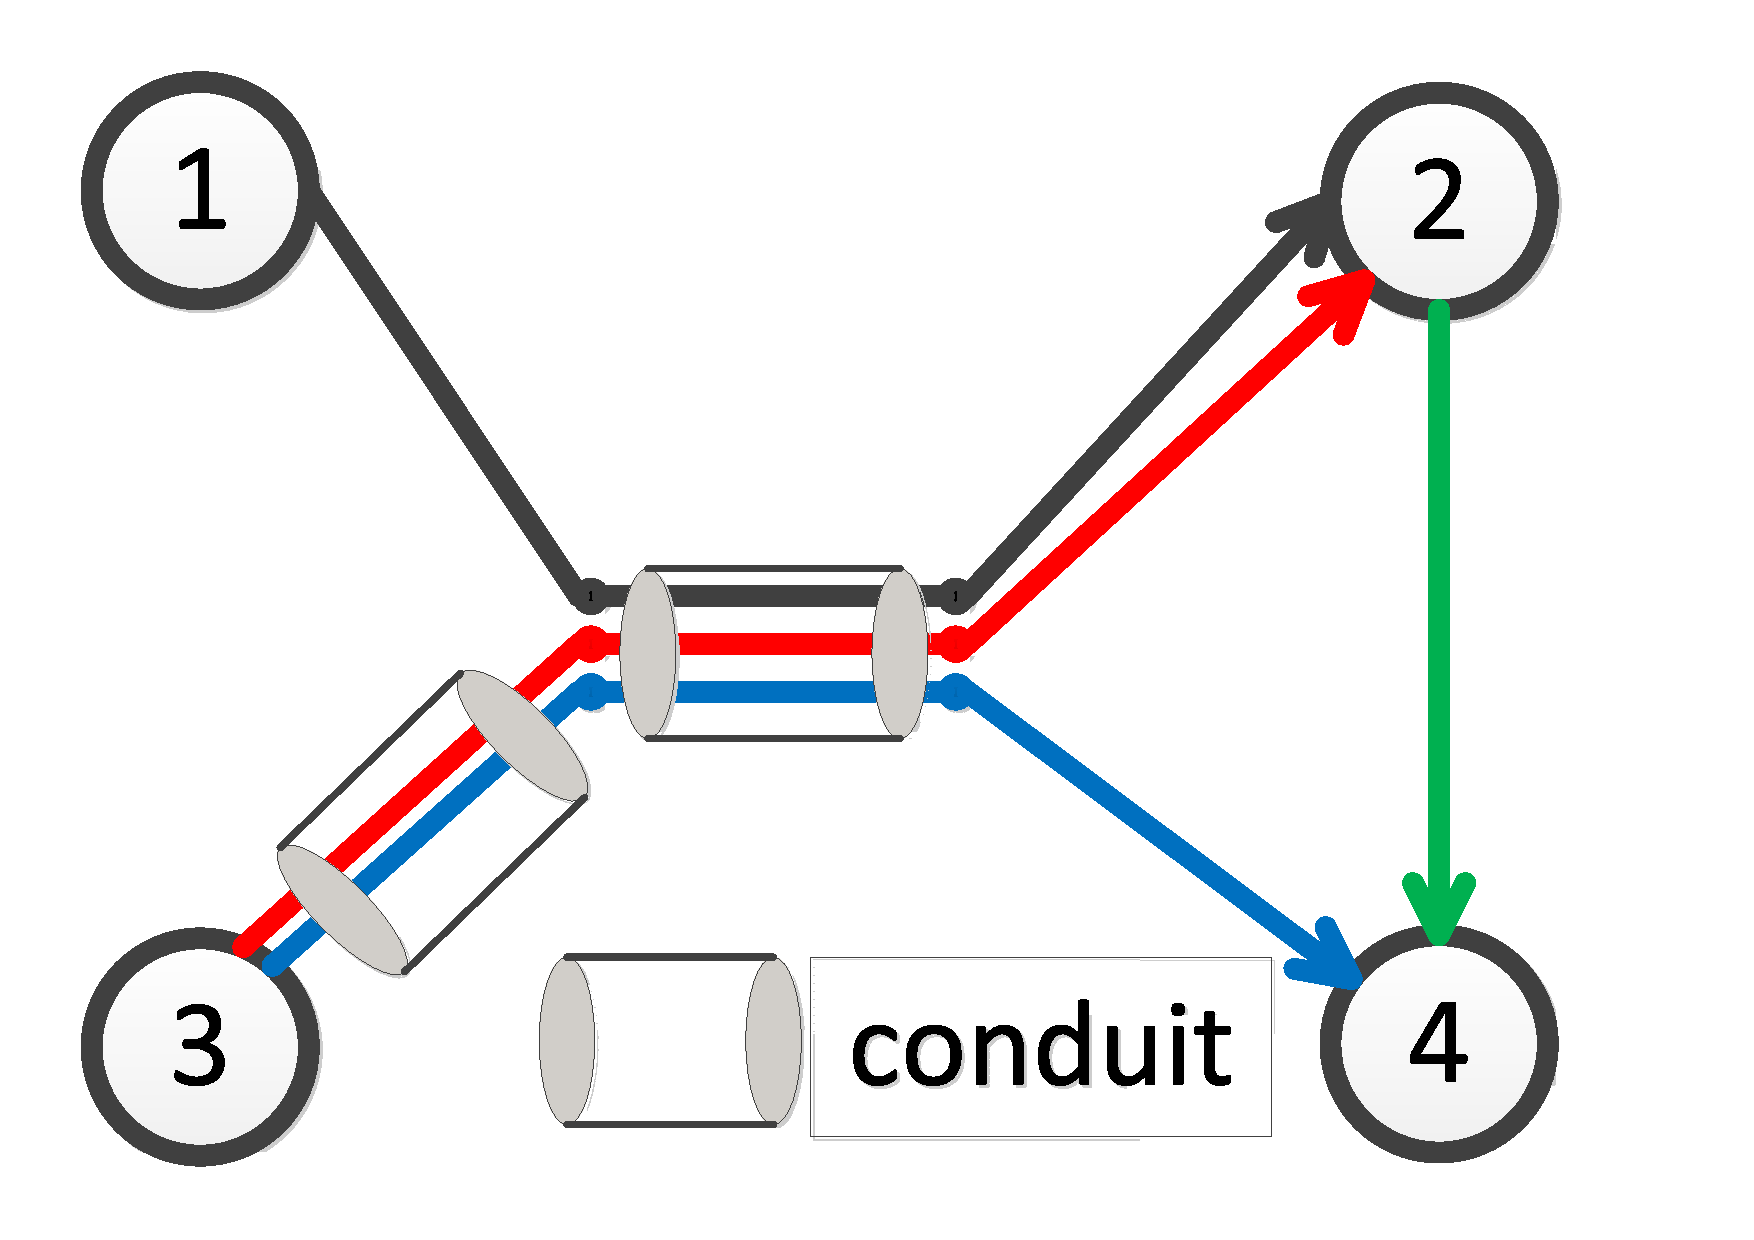
\includegraphics[width=1.25 in]{figures/PhysicalGraph}
}
\subfigure[Network Graph]{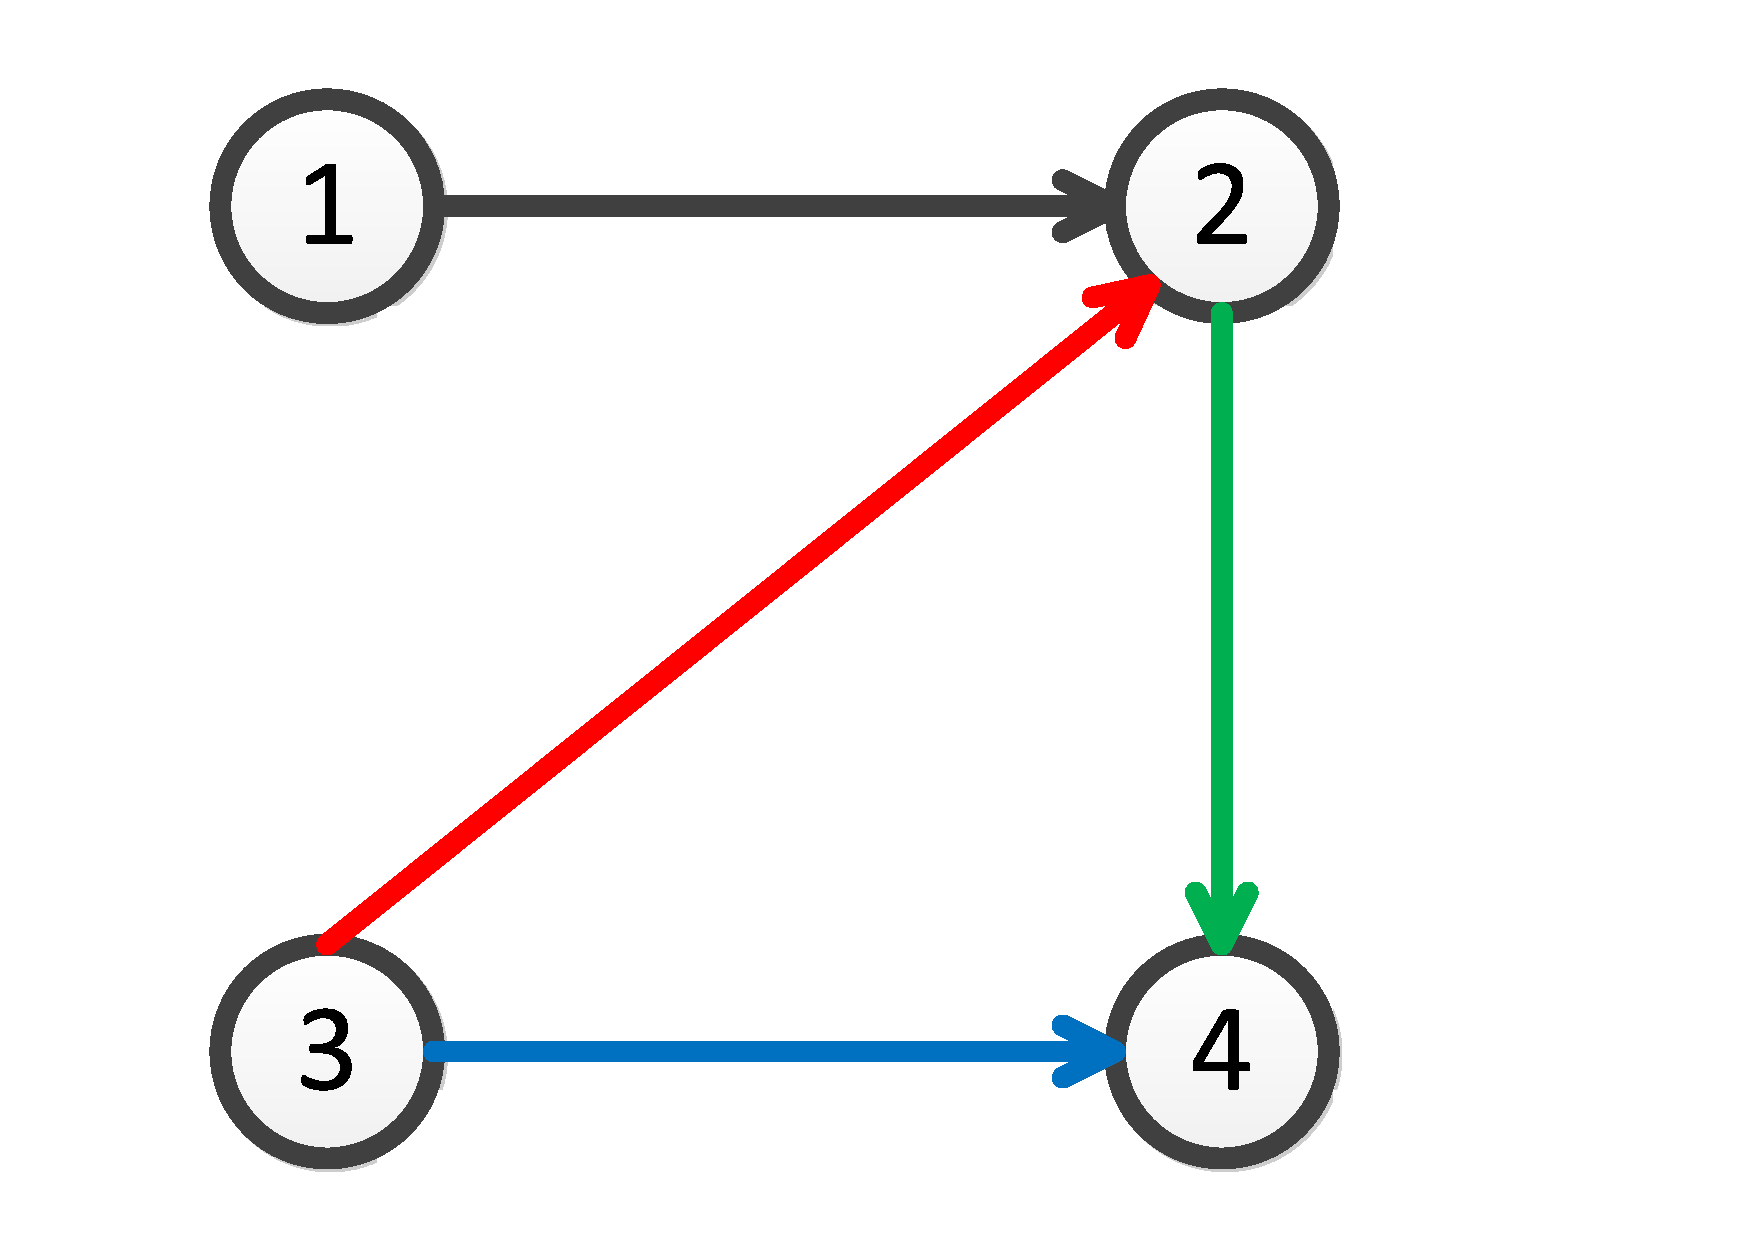
\includegraphics[width=0.9 in]{figures/VirtualGraph}
}
\caption{Example of shared risk link group(SRLG)}\label{fig:SRLGgraph}
\label{fig:Logic shift operation}
\end{figure}

设$\mathbb{R}$为网络中的风险集(故障)。每个风险可能对应于导管断开、光纤断裂、在一个节点上驱动故障、软件故障或这些因素的任何组合。对每一个共享风险链路组$r_i \in \mathbb{R}$是指与其风险$r_i$相关的链路集合$\mathbb{R}_{r_i}$,$1\leq i\leq \chi$ 和 $\chi=|{\mathbb{R}}|$是共享风险链路组集合的个数。图.\ref{fig:CompositeGraph}(a)所示,该图包含五个共享风险链路组集合$\mathbb{R}_{r_1}=\{e_1,e_9\}$, $\mathbb{R}_{r_2}=\{e_2,e_3,e_{19}\}$, $\mathbb{R}_{r_3}=\{e_2,e_4,e_{11},e_{17}\}$, $\mathbb{R}_{r_4}=\{e_5,e_{13}\}$, $\mathbb{R}_{r_5}=\{e_{15},e_{18}\}$。在这个例子中,链路$e_2$同属两个共享风险链路组集合里$\mathbb{R}_{r_2}$ 和 $\mathbb{R}_{r_3}$


$r_P$表示影响路径$P$上的风险集合,即$r_P=\{r\in \mathbb{R}$: 路径 $P$ 包含的链路在 $\mathbb{R}_r$中$\}$。如图.\ref{fig:CompositeGraph}(c)所示,在路径$AP$ 上的边集$\mathbb{AP}=\{e_1,e_2,e_3,e_4,e_5,e_6,e_7,e_8\}$,并且$e_1\in \mathbb{R}_{r_1}$, $e_2\in \mathbb{R}_{r_2}$, $e_2\in \mathbb{R}_{r_3}$, $e_3\in \mathbb{R}_{r_2}$, $e_4\in \mathbb{R}_{r_3}$, $e_5\in \mathbb{R}_{r_4}$,路径$AP$的风险集合是${r}_{{AP}}=\{r_1, r_2, r_3, r_4\}$。$\mathbb{\mathbb{ER}}$代表不属于$AP$上的链路但是与$AP$共享相同的风险集合的链路。如图.\ref{fig:CompositeGraph}(c)所示,$\mathbb{\mathbb{ER}}=\{e_9,e_{11},e_{17},e_{13},e_{19}\}$。




\subsubsection{最大网络流}
设$G=(\mathbb{\mathbb{V}},\mathbb{\mathbb{E}})$是一个网络(其中$\mathbb{\mathbb{V}}$是$|\mathbb{\mathbb{V}}|$个节点的集合,$\mathbb{\mathbb{E}}$是$|\mathbb{\mathbb{E}}|$条链路的集合),其中$s\in \mathbb{V}$和$d\in \mathbb{V}$分别指源节点和终节点。链路$e_i$ 的\textbf{容量}表示该条链路的最大流量。链路的流$f_{e_i}$应该满足以下两个限制:
\begin{enumerate}
  \item 容量限制: $\forall e_i\in \mathbb{\mathbb{E}}$: $f_{e_i}\leq c_{e_i}$.
  \item 流量守恒: $\forall u\in \mathbb{\mathbb{V}}-\{s,d\}$: $\sum\limits_{v\in \mathbb{V}}f_{(v,u)}=\sum\limits_{v\in \mathbb{V}}f_{(u,v)}$,  $(v,u)$ 和 $(u,v)$ 代表链路 $e(v,u)$ 和 $e(u,v)$.
\end{enumerate}

流的值定义为$|f|=\sum\limits_{v\in \mathbb{V}}f_{(s,v)}$,其中s是源节点。它表示从s节点到d节点的流量。\textbf{最大流量问题}:尽可能的求从s节点到d节点的最大流量值$|f|$。

一个 s-d 割${\Phi}=(\mathbb{S},\mathbb{D})$ 是节点$\mathbb{V}$的划分满足$s \in \mathbb{S}$ 和 $d \in \mathbb{D}$。$\Phi$ 的割集合$\mathbb{\mathbb{L}}_{\Phi}$是一个包含边的集合。
\begin{equation}
\mathbb{\mathbb{L}}_{\Phi}=\{(u,v)\in \mathbb{E}: u \in \mathbb{S}, v \in \mathbb{D}\}.
\end{equation}

如果在割集合$\mathbb{\mathbb{L}}_{\Phi}$中的边被去除,那么在原图中的流值$|f| = 0$。即没有流能从s节点到d节点。一个 s-d 割${\Phi}=(\mathbb{S},\mathbb{D})$的容量被定义成$c(\Phi)=\sum\limits_{e_i\in \mathbb{\mathbb{L}}_{\Phi}}c_{e_i}$。\textbf{最小s-d 割 $\Phi$ 问题},最小化$c(\Phi)$即决定点集$\mathbb{S}$ 和 $\mathbb{D}$使得s-d割${\Phi}=(\mathbb{S},\mathbb{D})$的($c(\Phi)$) 最小化 。

\textbf{最小割最大流定理}:一个s-d流的最大值等于s-d割的最小割。如图.\ref{fig:FlowNetwork}所示,在图$G$中的流量$|f|=f_{(s,v_1)}+f_{(s,v_2)}$。这个割$\Phi(\mathbb{S},\mathbb{D})$ 是 $\mathbb{S}=\{s,v_1,v_2,v_4\}$ 和$\mathbb{D}=\{v_3,d\}$,它是最小的割其容量为$c(\Phi)=c_{(v_1,v_3)}+c_{(v_4,v_3)}+c_{(v_4,d)}=12+7+4=23$. 显然, $|f|=c(\Phi)$, 即s-d 最大流等于所有s-d割中最小的容量。
\begin{figure}[htbp]
  \centering
  % Requires \usepackage{graphicx}
  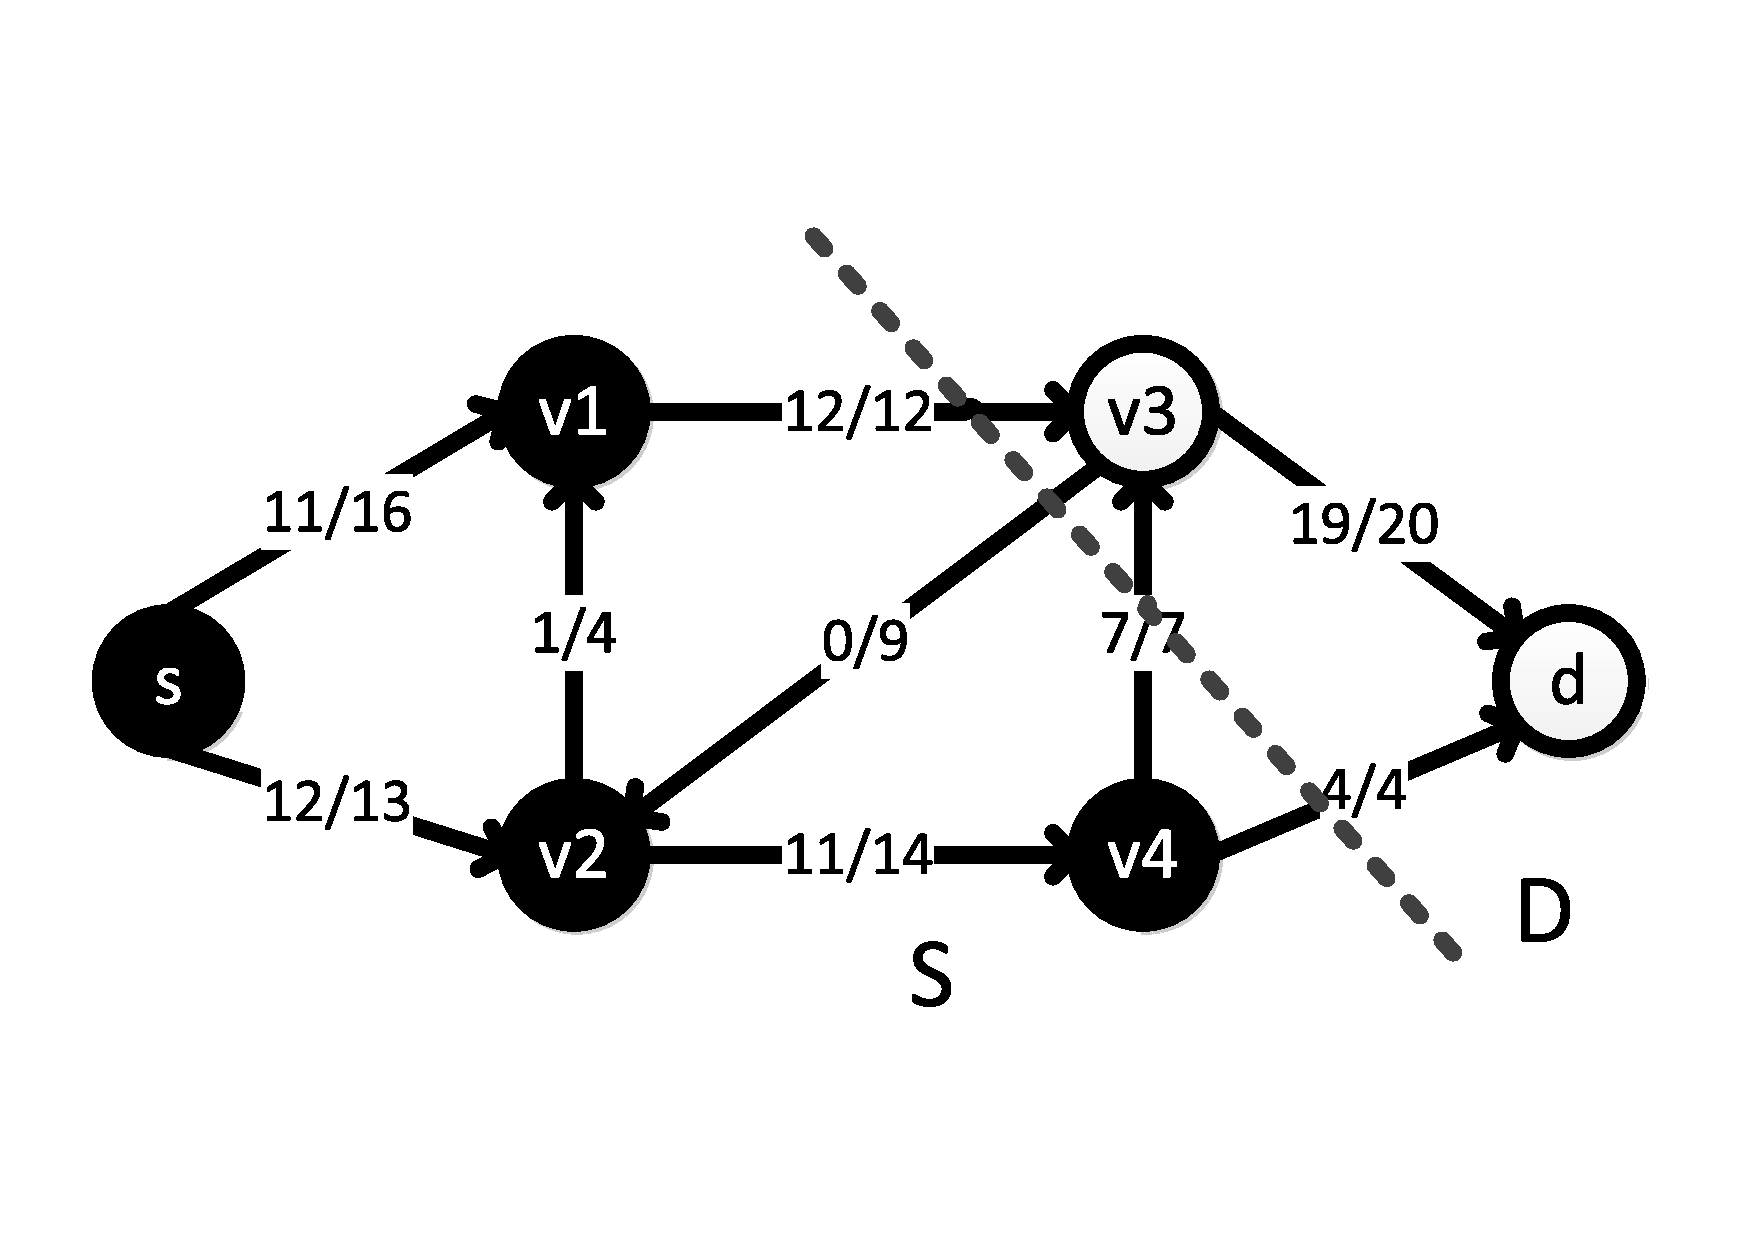
\includegraphics[width=2.5in]{figures/FlowNetwork}\\
  \caption{An example to illustrate max-flow min-cut theorem. Each link $e_i$ is labeled by $f_{e_i}/c_{e_i}$, where $f_{e_i}$ and $c_{e_i}$ denote the flow and capacity of link $e_i$, respectively.   }
  \label{fig:FlowNetwork}
\end{figure}

\subsection{计算理论}

\section{相关的研究及发展趋势}
\section{论文的主要研究内容和组织结构}
\subsection{论文的主要研究内容}
\subsection{论文的组织结构与贡献}
本文依据SDN、路由算法以及分离路径。。等方面的研究现状与发展趋势,并结合自身对以上的研究和探索,将本文分为五章,各章主要内容如下:
\begin{itemize}
  \item 第一章为绪论部分,主要介绍了本课题的研究背景及其意义并且简要地分析了国内外研究现状和发展趋势。
  \item 介绍
  \item 介绍
\end{itemize}



% !Mode:: "TeX:UTF-8"

\chapter{网络可生存性的基本原理}
为了增强网络性能、保证网络的健壮性,需要对网络中(本文以软件定义网络为研究背景)的许多问题进行优化设计,这些问题主要包括:网络可生存性设计问题;业务恢复问题等。随着网络业务爆炸性的增长及在各个领域的广泛应用和SDN网络的兴起,网络生存性问题已成为SDN网络关注的焦点。目前业内提出了许多关键词,比如可靠性、抗毁性、鲁棒性和可信赖性等,它们的本质都是以网络生存性的研究为出发点。在本章中我们主要就网络可生存性问题展开讨论。



\section{网络的可生存性概述}
软件定义网络中控制层中心控制器管理每条信道,而当某条信道发生故障,则必须在短时间内恢复。因此在软件定义网络网络控制层路由方面,研究路由的生存性变得尤为重要。

关于网络可生存性(survivability)具体定义有多种说法\cite{al2009comparative}。1993年 Neumann\cite{hollway1993survivable}等人正式提出网络系统可生存性定义:在任意的不利条件下,基于计算机通信系统的应用应具有持续满足用户需求的能力,其中用户需求包含安全性、可靠性、实时响应和正确性等需求;1999 年 Ellison\cite{ellison1997survivable}等人进一步完善了网络系统可生存性的定义:网络系统在遭受攻击、故障和意外事故的情况下及时完成任务的能力,属于网络完整性的一部分。

考虑到今天通信系统和基础设施的重要性,网络应该在设计和操作上考虑到系统或者设施出现故障能够被解决。例如,由于恶意攻击,自然灾害,突然间的电缆断裂,计划维修,设备故障等等,网络节点/链接可能出现故障。弹性,容错性,可生存性,可靠性,鲁棒性和可信赖性,是已经被使用的不同术语。这些术语是面对网络故障时网络维护运行保持通信能力的术语。如作者\cite{al2009comparative}所指,不同的术语有重叠的意思和一定的歧义。在本文中,我们将使用可生存网络一词是指在网络当一个网络组件出现故障,可以通过找到替代路径来避免使用故障的网络组件。

随着人们对生存性技术的关注,国内外的许多研究机构都对其投了大量的人力、物 力,其研究重点可概括为可生存性的基本概念\cite{kuipers2012overview}、可生存性体系结构、系统模型\cite{luxinhua2006}、 系统分析与设计、系统工程方法和工具、生存性风险评估\cite{linxuegang2006} 等。

就国内目前的研究来看,网络生存性设计主要基于两种模式\cite{hanjianjun2007},即基于入侵使用情景 的重新设计和基于入侵容忍技术的生存系统设计方法。简单来说,第一种模式是在故障产 生后对系统模型的重新开发,目前还处于研究阶段;而第二种模式采用了容忍入侵的策略,它具有高效的监测系统,一旦发现故障,便调用冗余资源进行系统异常修补。第二种模式 的代价较第一种模式要高一些,并且现阶段的研究还不是很成熟,目前比较经典的是基于 入侵检测技术的设计模式,它通过对网络故障的快速检测、定位和恢复使其可靠性提高。

现阶段,网络生存性研究已经得到了很大重视,很多知名学者就该问题的不同方面作了深入研究,问题涉及故障分类、生存性建模分析、故障恢复技术、生存性网络规划 等许多子领域,并取得了一些成果。三种方法是能使网络达到可生存性能力。
\begin{enumerate}
\item 网络连通,即可生存性好的网络应该是高连通性的。
\item 网络增强,即可能需要新的链路以增加网络的连通性。
\item 路径保护,即寻找替代方案的过程,失败故障时的替代路径。
\end{enumerate}


现实网络中网络故障是不可避免的,因此必须加强网络可生存性研究,可以采取对网络故障进行快速的检测、定位和恢复的方式,以保证网络的可生存性。


\section{网络可生存性指标}
本文在进行网络生存性设计时,要达到的最理想的状态是:对于给定的网络拓扑结构, 能够在最短的时间内使故障元素获得最大程度的恢复,并同时保证最大的资源利用率。然而由于事件的互斥性,很难同时实现所有这些要求,所以需要根据不同的业务或用户需求 以及网络本身的特点,采取相应地措施,从而满足网络的生存性指标要求。

常用的网络生存性指标主要有:
\begin{itemize}
  \item 故障恢复时间:是指从网络故障发生时,到业务恢复正常传输所需的时间。该 项指标最直接,也最能体现网络的生存性能力。众所周知,对于网络用户来说,传输过程 是透明的,他们所能感受到的就是网络提供的业务服务质量,而其中最敏感的因素便是故 障恢复时间。
  \item 业务请求拒绝率:是指被拒绝的网络业务数最与总体业务请求数量的比率。可生存性网络研究的目标是最小化请求拒绝率。
  \item 平均网络负载:网络负载是指网络链路中的流量负荷,一且链路负荷过重,将直 接影响整体网络的迕通性。因此,最小化网络负载将有利于网络生存性的研究。
  \item 业务平均跳数:某些网络有时以步长来衡量代价耗费,因此最小化路径长度是网 络优化指标之一。
  \item 网络资源利用率:这是衡量任何一个网络优劣的可靠指标,提高网络利用率是网络运营商追求利益的根本。
  \item 鲁棒性:即健壮性,是指经历过一次网络故障后,网络再次承受故障的能力。它主要用来衡量网络业务的可持续性。
\end{itemize}
其中,网络资源利用率、业务请求拒绝率和平均网络负载是几个最常用的评价指标。


\section{网络故障分类}
由于遭受破坏的因素及网络元素不同,网络故障也是多种多样,按照光网络中故障的 表现方式不同可分为软故障和硬故障;按照故障产生的元素不同可分为信道故障、节点故障和链路故障。概念解释如下:

所谓硬故障是指某些意想不到的突发事件致使传输信道中断的事件,如地震、光纤断 裂、收发元器件失效等;软故障是指传输过程中由于信号逐步衰减,而造成信息丢失的事 件,如光纤损耗増大等。

不难看出,硬故障对网络业务影响较大,但处理方便;软故障对网络业务的影响比较小,但出现机率较高,不容易被发现,并且难以对故障精确定位。

因而,从科研角度出发,光网中的故障按位置区分更利于研究:
\begin{itemize}
\item 信道故障是由于该信道对应的特定激光器或接收器出故障引起。
\item 链路故障主要是由于光纤断裂引起。
\item 节点故障主要是由于断电或是地震等灾难性情况引起。
\end{itemize}

网络故障主要表现为链路故障,链路故障恢复策略可分为主动式和被动式两种\cite{kvalbein2009multiple}。被动式策略在网络故障后动态自适应地进行全网资源重分配,但
路由重新收敛花费较多的时间而不可接受。因此目前故障快速恢复研究以主动式策略为主,通过提前对网络进行资源规划和预留,使得故障时能迅速切换,如基于多拓扑\cite{shand2010ip}和基于备份路径的故障恢复技术。多拓扑技术需要配置多个拓扑子层,路由存储消耗大;基于备份路径的故障恢复技术提供端到端路径重路由,在全局范围内进行流量分配,易于基于现有协议实现。因此,备份路径技术是当前故障恢复领域研究的热点\cite{yang2014keep,suchara2011network,banner2010designing}。

\section{网络故障恢复}
网络的生存性实现机制根据是否预留备用资源和是否进行重路由计算,通常把故障处 理策略分为保护(protection) 和恢复(restoration)f311两种。保护措施和恢复措施均是在 网络故障情况下,使受损的业务得以重新运行。原理上,两者均利用重路由方式(重新选 择新的路由来代替故障路由),继续故障业务数据传输。就具体实施方案而言,保护和恢 复方法又有所不同。两种方案各有利猝,恢复机制能够提高网络资源的利用效率;保护机制可提供更快的恢复时间,有利于网络QoS的保障。下面我们将做详细区分。

所谓保护方案是指,事先为业务分配好预留的保护资源即备份资源,主要利用节点 之间预留的备用资源来实现网络保护。当故障发生时,业务可以由事先预留的保护资源承 载,即将工作通路上的通信信号倒换到备用通路上,使工作信号通过预留的保护通路维持 业务正常传输;而恢复方案指,并不事先为业务分配预留的保护资源,在检测到故障时, 动态地从网络中寻找替代的路由,来承载受故障影响的业务。如果此时找不到合适的路由,那么,该工作路径上携带的业务就会丢失。

两种方案对比如下:
\begin{itemize}
  \item 由于保护机制是事先对特定的故障做了假设,进而预留了备份资源。它能够确保 对于预料之中的故障(如单链路失效〉业务的恢复,而对于些未知故障(如多链路同时 失效),则不能确保其恢复能力。
恢复机制是在发生故障后实时、动态地寻找可用资源,这种方式灵活性较强,W以针 对多种失效情况进行恢复,特别是对于多链路同时失效下的恢复。但由于事先没有预留备 份资源,因此在很多情况下,网络的资源状况不能确定,也就无法确保及时恢复。
  \item 保护机制是在牺牲资源利用率的前提下实施的,因而可以较快的实现业务恢复;恢复机制是动态地根据当前网络状态重路由,从而可以实现较高的资源利用率,但业务恢复 时间较长。
\end{itemize}
由上面的阐述可见,保护和恢复方案两者不存在互斥现象,因此,我们在进行网络的 生存性设计时,往往会考虑将保护和恢复方案折中的办法,取两种方案中的优点合并,从 而为客户提供多种服务级别,尽可能做到在恢复时间、运行保障与效率及成本之间取得平 衡。同时保证故障情况下,时效性和网络资源的合理化利用,即保证在一定的约束下为工 作通路预先选择好保护通路。这就相当于以网络生存性为约束条件的资源优化的问题。

一般而言,运营商根据不同的服务标准,对不同业务选择不同的方案,选择依据如下:
\begin{itemize}
  \item 对于重要的业务,如金融业,一般采取保护的方案。
  \item 对于一些特殊的拓扑,如链形、环形或环网相交等可以采用保护方案。
  \item 对于网络拓扑连通性强,且对网络的资源利用率要求较高的一些网络,则可以选
用合适的恢复方案。
\end{itemize}

由于现实中网络资源的不足,在实际的网络操作中,通常以保护机制为基础,來保 障一些可预料的故障,(如光缆断裂等公共失效故障〉,然后,再使用恢复机制进行加强,保障整网范围内的故障或失效。根据不同要求的业务可以选择不同类型的方法以保证其生存 性,例如对于实时业务,可以使用链路/节点保护,即预先建立保护通道和预留资源的保护 方式;而对于“尽力而为”的业务,就可以按需建立保护通道,或者依靠高层的恢复机制。 与恢复机制相比,保护机制具有更高的可靠性和更快速的恢复能力,这更适用于具有巨大 传输容量的光网络,因此本文主要研究的是保护机制。
\section{网络保护策略}
随着技术的发展,网络所承载的信息流量显著增加,特别是在主干网中,网络中设备 接口的速率达到2. 5Gb/s 以上,即使仅持续几秒的短暂性故障也会造成大量的数据丢失。 因此,为故障的业务寻找新的传输路由,并使其在尽可能短的时间内自愈变得越来越重要。 目前,许多文献对于光层故障保护方案进行了大量的研究,根据不同的功能或方式总结如下:
\begin{itemize}
  \item 从重路由的角度分为:基于路径保护、基于链路的保护及区段保护。
  \item 根据备用资源的预留方式可分为:专用保护和共享保护。
  \item 按照路由的计算方式可分为:预计算和实时计算。
\end{itemize}
\subsection{路径保护}
所谓通道(路径)保护M是指业务故障恢复由通道两端的终端节点来完成。具体说来, 基于通道的保护机制是指对工作路由事先预留一条备用保护路由,在故障发生后,用预留的保护通道来传输故障通道中的业务流,从而取代故障通道,实现业务重路由。在通道保 护方案中,每条光路在建立时就己经预设了一条端到端的备用通道并预留了备用资源。一 且网络中发生故障,受到影响的通道的源-目的节点对间的业务流将自动由工作通道切换 到这两个节点间的另一条与故障通道链路不相交的备用通道上来,从而保证业务恢复。即 当发生故障时,其切换过程只涉及源、目的节点,与中间节点无关,由于是源节点和目的 节点启动保护倒换,因而对故障的具体定位要求不高,但信令协议必须快速准确的将故障 消息传送至源、目的节点。工作状态如图2. 4所示:

通道保护又可分为专用通道保护(备用资源为某条工作通道专用)和共享通道保护(备 用资源能同时为多条工作通道提供保护)。专用保护通常是指1+1通路保护和1: 1通路 保护。共享保护是指1: N保护方式。
\subsection{链路保护}
基于链路的故障保护方案,是指业务请求经过的每一条链路,都有一条保护路径对其 进行保护,一旦链路出现故障,业务将越过故障点,直接转到保护路径上。它是通过处理 与故障点相邻的节点来实现对业务的恢复的,是将受故障影响的业务流绕过故障链路来进 行重路由。即:在与故障点邻接的两点间,为该故障链路寻找一条可绕过该故障点的备用 路由。显然,该保护方案中,参与保护切换的节点数较少,因而具有较强的本地性,恢复 速度较快。同时由于它的本地性,也使得资源浪费过多,从而,无法有效的利用资源。
在该方案中,对于不同链路中的业务,只要不同时发生故障,就可以共享相同的保护 路径,因此也可以分为专用链路保护和共享链路保护两种。前者是指对于某一链路,提 供专门的保护路径,其他链路则不得使用该专用路径;而后者允许不同的链路保护路径在 其重叠的部分实现共享。比较而言,后者比前者资源利用率要高,而前者较后者的保护力 度大。
\subsection{区段保护}
区段保护是折中了通路保护和链路保护各自的特点而得到的一种中庸的保护方式。区 段保护是指在一对节点之间出现光纤断裂故障时,则该段链路中的业务被倒换到这两个节点之间的另一根光纤中。如果两个相邻节点之间的一根光纤发生断裂,则类似于链路保护。
\subsection{本章小结}
网络生存性设计的目的是提高网络的健壮性,由于网络故障不可避免,那么故障后的 及时修复成为网络性能的一个重要方面。本章给出了故障业务恢复方法的综述,比较得出共享保护方案优于专用保护方案,同时通道保护方案优于链路保护方案,由此提出,一般 共享通道保护方案的性能较高。



%在满足delay 约束的同时达到两条路径总的
%花费(cost)最小.当给定的delay 约束针对两条路径的端到端延时总和时,问题被称为DCLDOP-I(delay
%constrained link disjoint optimal paths),当给定的delay 约束针对路径对中每条路径的端到端延时时,问题被称为
%DCLDOP-II.文献[Researches on the problem of link disjoint paths with QoS constraints]对DCLDOP-I 和DCLDOP-II 问题进行了建模,证明了这两种问题同属于NP 完全问题.文献
%[4]针对DCLDOP-I 问题提出了两种近似求解算法.文献[Constrained shortest link-disjoint paths selection: A network programming based approach]研究了总延时受限下的k 条cost 最小链路分离路径
%问题.文献[On the complexity of and algorithms for finding the shortest path with a disjoint] 提出了Min-Min 问题,旨在求解两条满足QoS 约束的分离路径且满足较短的路径cost 最小.文献[Link-Disjoint shortest-delay path-pair computation algorithms for shared mesh restoration networks]
%通过求解总延时最小的链路分离路径对来解决单链路失效后的路由恢复问题.

\chapter{分离路径问题}
网络在我们的日常生活中非常普遍。我们的身体由突触连接的神经元网络。我们的运输网络使我们能够轻松地往返于不同的地方。互联网是我们巨大的信息门户也是世界范围内的计算机网络。电网提供电力,而如果没有电力那我们现在社会可能会停止运作。我们的社交网络让我们和朋友和家人约会。由于网络的重要性,网络特性的多样性已经得到了广泛的研究,尤其是在图论领域。在图论中,网络被看作是一种通过链接互连的节点。节点表示网络的关节点,例如,通信网络中的路由器,海运网络,或交通网络中的城市。链接表示将关键点连接在一起的连接器,例如,通信网络中的电缆,海运中的贸易路线,运输网络中的网络或公路。图论中研究最多的课题之一是最短路径问题,即在网络中的两个节点,使得路径上链路权重之和最小化。传统的最短路径算法是Dijkstra算法[1]以及Bellman-Ford算法[2,3]。使用最短路径,信号可以在最小延迟之间交换在一个通信网络的两个路由器间,货物可以在海运网络中两个港口之间的以燃油成本最低的代价发送,而且在运输网络中我们可以更快地往返于城市之间。不相交路径(Disjoint Path)问题可以看作是一个扩展。最短路径问题。而不是只有一个单最短路径,几条不共享任何公共路径的路径计算链接(或节点)。提供不相交的途径网络流量将提高网络连接的可靠性,相应的网络生存性。网络生存性定义为网络的能力在网络组件存在的情况下提供持续的服务(例如,节点和/或链路)故障[4]。另一种变体不相交路径问题是不相交路径对问题,其中,而不是为单个对象找到多个不相交的路径。
对源节点和目标节点,计算单个路径。
对于每一对源节点和目标节点,这样的
道路是不相交的。
不相交路径有广泛的应用。例如,
在通信中具有多条不相交的通信路径
网络将提高其传输可靠性。通过
在多个不相交路径上并发发送通信量,则
路径的失败不会影响其他路径的性能。
路径,流量仍然会到达目的地。在运输中
网络,具有预先计算的不相交数。
路径将使卡车司机能够遵循不同的路径
改变风景而不是总是坚持最短的
路径。

%maritime network freights

本文的其余部分按以下方式组织。在不相交路径部分,给出了不相交路径的形式化定义。路径问题,讨论不相交的附加条件路径问题及其相应的复杂性解释几种有代表性的不相交路径算法。在基于可用性的不相交路径部分,我们将介绍路径可用性的概念及其与不相交路径的关系问题。最大不相交路径部分阐述在不相交路径可能部分重叠的情况下,而不是完全不相交。我们继续寻找不相交的地方域中多域网络上下文中的路径-不相交路径部分。因为多个链接(或多个节点)可能在类似的分担风险下同时失败,分担风险链接组(SRLG)-不相交路径部分介绍共享风险链接组的概念,并解释方法。确保不相交的路径不会同时失效由于单个链接(或节点)失败。风险也可能影响基于区域的网络,因此区域-不相交的路径本节讨论了几种基于区域的风险模型及其相应的风险模型。寻找区域的方法-不相交路径。阿与不相交路径问题对应的不相交路径对问题将在不相交路径对部分中讨论,的复杂性讨论了不相交路径对问题。最后,我们给最后一节对论文进行了简要的总结。
\section{完全分离路径}
\section{基于可靠性的分离路径}
\section{最大分离路径}
\section{范围分离路径}
\section{共享风险链路组分离路径}
\section{共享风险节点组分离路径}
\section{区域分离路径}
\section{分离路径对}

\chapter{共享风险链路组不相交路径算法}

\section{问题描述}
SRLG不相交路径在它们之间没有任何共同的风险资源,也就是说,由于风险而导致的路径失败不会影响其他路径。图.\ref{fig:CompositeGraph}(b)显示两条SRLG不相交路径对,表示为AP 和BP. 因为这两条路没有共同的风险资源,如果AP 失败,BP仍然可以工作。本章主要讨论了两条不相交的路径保护路径,即可以描述如下。

\textbf{Min-Min SRLG不相交路径问题}。给定一个图$G(V,E)$,每条链路$e_i\in \mathbb{E}$ 相关联一个权重权重$w_{e_i}$,一个源节点$s$和一个终结点$d$,找到一对$s$ 到$d$ 的SRLG不相交路径对(表示为AP和BP),而且要求这两条不相交路径中路径权重较小的那条路径权重最小化,形式如下:

\begin{equation}
\begin{array}{*{20}{c}}
   {\mathop {minimize}\limits_{AP,BP} } & {\min \left( {{w_{AP}},{w_{BP}}} \right)}  \\
   {subject\ to} & {{r_{AP}} \cap {r_{BP}}{\rm{ = }}\phi }  \\
   {} & {\mathbb{AP} \cap \mathbb{BP}{\rm{ = }}\phi }  \\
\end{array}
\label{eq:problem definition}
\end{equation}

即${w_{AP}}$ 和 ${w_{BP}}$是AP和BP的路径权重,$\mathbb{AP}$ 和 $\mathbb{BP}$分别是路径AP和BP上的链路集,${r_{AP}}$ 和 ${r_{BP}}$分别是影响路径AP和BP的SRLG 集。


\begin{figure*}[tp]
  \centering
  % Requires \usepackage{graphicx}
  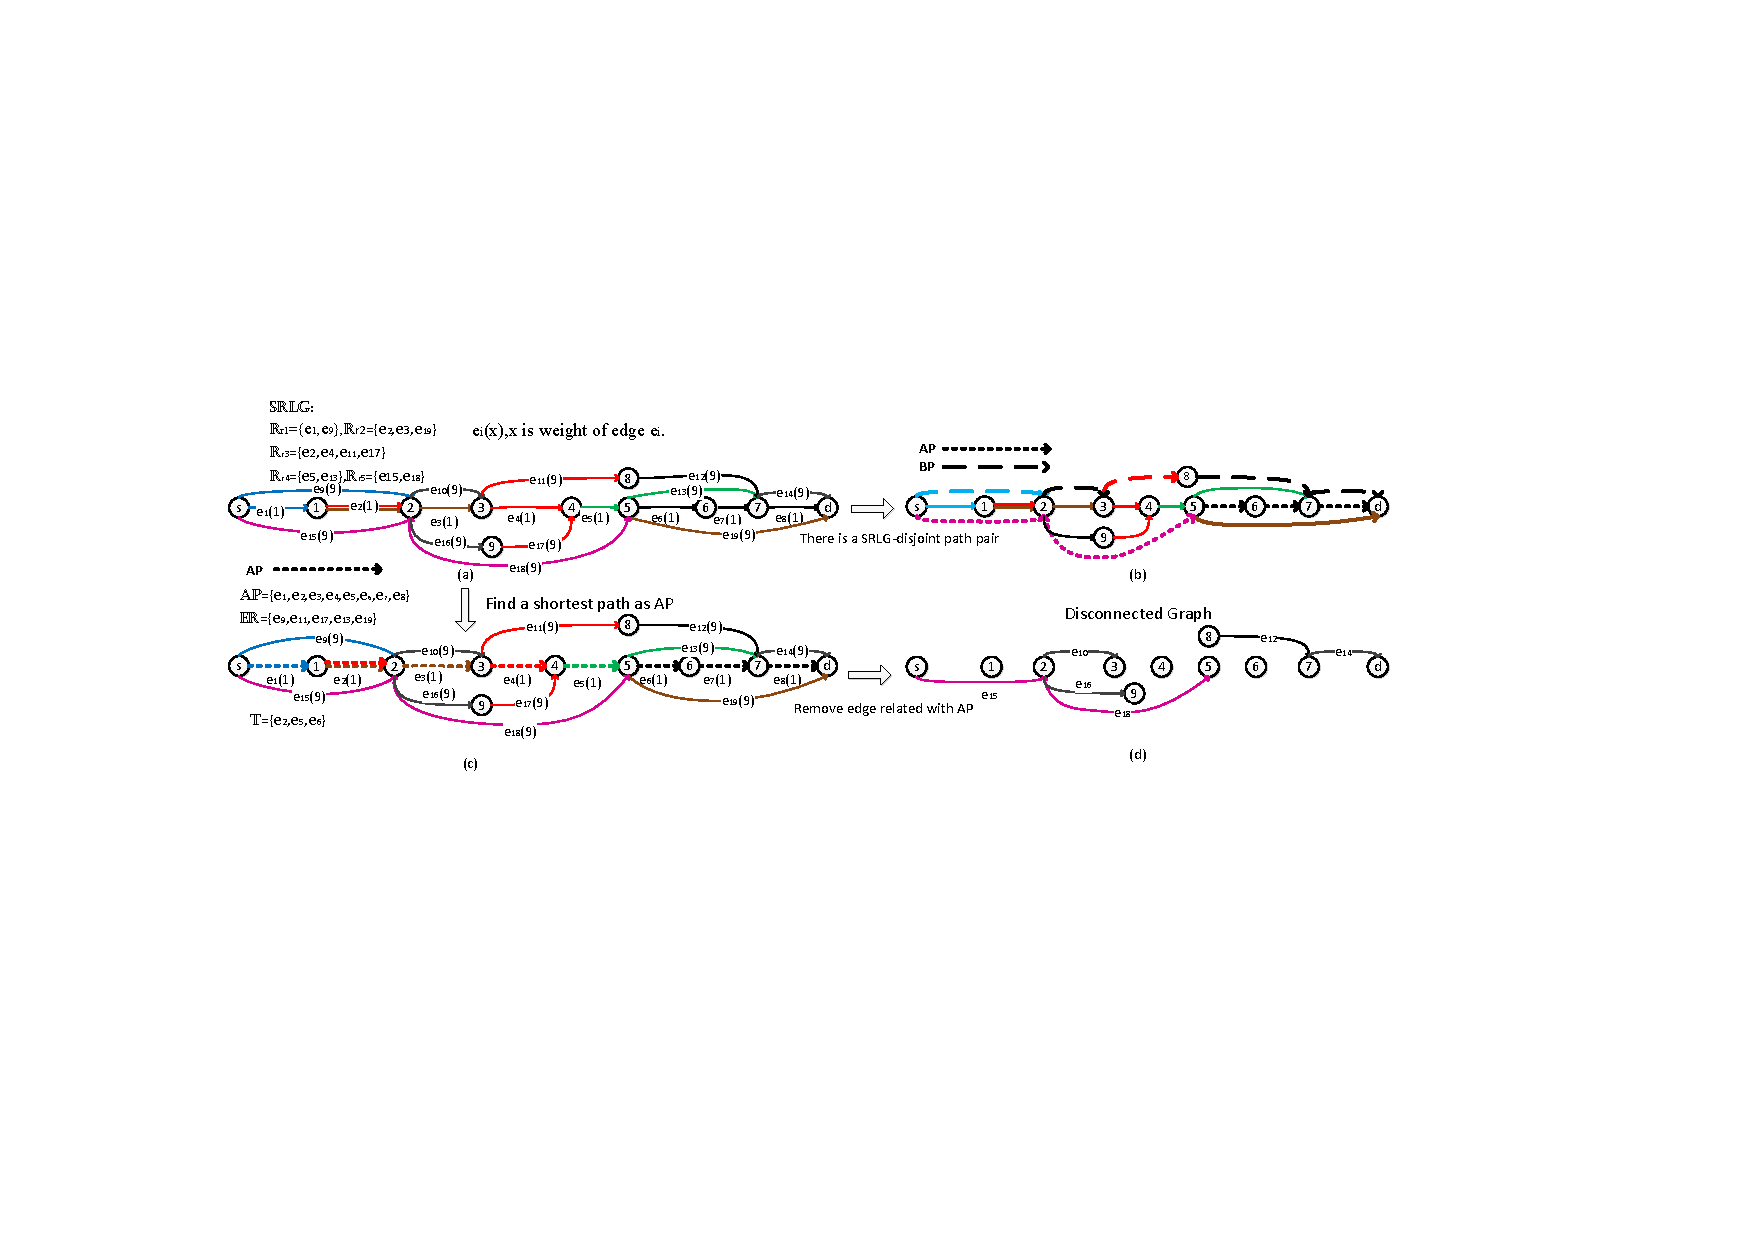
\includegraphics[width=7.2in]{figures/CompositeGraph}
  \caption{(a) A graph with five SRLGs: $\mathbb{R}_{r_1}=\{e_1,e_9\}$,$\mathbb{R}_{r_2}=\{e_2,e_3,e_{19}\}$,$\mathbb{R}_{r_3}=\{e_2,e_4,e_{11},e_{17}\}$,$\mathbb{R}_{r_4}=\{e_5,e_{13}\}$,$\mathbb{R}_{r_5}=\{e_{15},e_{18}\}$. (b)AP and BP in the graph. (c) The shortest weight path AP in the graph. $\mathbb{AP}=\{e_1,e_2,e_3,e_4,e_5,e_6,e_7,e_8\}$, $\mathbb{\mathbb{ER}}=\{e_9,e_{11},e_{17},e_{13},e_{19}\}$. (d)  Graph after deleting the links in $\mathbb{AP}$ and ${\mathbb{ER}}$. }
  \label{fig:CompositeGraph}
\end{figure*}

\section{原有算法概述}
共享风险链接组(SRLG)是一组链路共享相同的一个组件,该组件的故障会导致在这个组里所有链接的发生故障。就路径保护而言,尽管某些链路或者节点不相交路径算法\cite{suurballe1984quick,bhandari1997optimal,li1990complexity,guo2003link,xu2004finding,beshir2011variants,guo2013finding,hu2003diverse} 已经提出来,SRLG不相交路径 问题是比较棘手的,而且这些原有研究是限制在一定领域的。比如当每个SRLG只包含一条链路时,这个SRLG不相交路由问题可以简化为链路不相交路径问题,而通过节点不相交方法(node split method)\cite{ford2015flows}节点不相交路径问题可以转化为链路不相交路径问题。因为SRLG组通常包括的链路超过一条并且网络中的链路通常可以属于多个SRLG组里,以至于求一对SRLG 不相交路径问题比求一对链路或者节点不相交路径问题要困难得多。

为了解决SRLG不相交路径问题,一种可能的方法是0-1整数线性规划(ILP)\cite{hu2003diverse},通过分支限界法(branch-and-bound)来搜索来选择最优的主路径和备份路径。该方法时间复杂度高,不适用于大型网络。为了降低算法的复杂度,基于APF的启发式算法\cite{oki2002disjoint,li2002fiber,eppstein1998finding}能够求Min-Min SRLG不相交路径问题的近似最优解。首先使用Dijkstra算法(或任何其他最短路径算法)求出主路径,求主路径时不考虑其相应的备用路径情况,在删除AP沿线的链路并且与AP共风险的节点和链路后,再利用最短路算法求的备用路径。

然而,使用APF启发式算法的有一个主要缺陷,一旦求得路径AP后也可能无法找到相对的SRLG不相交路径BP,即使网络中确实存在一对不相交路径。这就是所谓的“陷阱”问题,即使稠密网络中\cite{laborczi2001solving}这也是可能发生,在一个稀疏连接的网络中当然不能被忽略。陷阱有两种:不可避免的陷阱和可避免的陷阱。不可避免的陷阱是受拓扑约束的,任何算法都无法解决。如果网络不是2-边连通度的,则没有算法可以保证在拓扑中存在两个SRLG不相交路径。另一方面,当两个节点之间存在SRLG不相交路径对,但由于路由算法的缺陷而找不到时,就会出现一个可避免的陷阱。在本章中只考虑了可避免的陷阱。

对简单的APF算法的扩展,提出了KSP(K-最短路径)算法来处理节点/链路不相交路径的陷阱问题。虽然它是处理陷阱问题最有效的算法之一,但它在大型网络中的性能受到影响,因为KSP 可能会涉及多路径搜索测试(K测试),直到它找到不相交路径。当前候选的路径AP遇到陷阱问题后,仅根据路径长度选择下一个要测试的候选AP,而不考虑当前候选AP的那条链路(或那些链路)导致查找不相交路径BP失败。因此,为了找到一对不相交路径对,需要对大量的路径进行测试,这就引入了KSP算法中与K相关的时间复杂度。对于遇到陷阱问题的AP,我们应用从AP 路径导出的SRLG冲突链路集来指导将来的AP路径测试。这在很大程度上有助于减少寻找替代路径的时间复杂度。

其它SRLG不相交路径算法\cite{rostami2012msdp,rostami2007cose,datta2008graph,xu2003new,todimala2004imsh},搜索最大SRLG不相交路径对,并且路径间共享最小数目的公共链路。由于AP 和BP 可能具有相同的风险资源组,通过这种方法找到的解决方案是不可靠的。我们的算法目标是寻找完全SRLG不相交路径。Xu\cite{xu2003trap}试图找到完全SRLG 不相交路径。但他的算法减少了问题的搜索空间,加快了路径搜索的速度。然而,它可能会以较大的代价返回路径,因为在削减后的空间可能会失去最优解。相反,为了大大加快搜索过程,我们利用SRLG冲突链接集将原问题划分为多个子问题,这些子问题可以并行执行。因此,我们的算法可以运行得更快,返回主路径成本非常低。

Datta\cite{datta2008graph}提出方法是将SRLG不相交路径问题转化为链路不相交路径问题,然后利用链路不相交路径算法来解决。然而,只有特殊的SRLG模式(例如,星型)可以
将其转换为链路不相交,这样就限制了该算法的广泛应用。当AP遇到陷阱问题时,CoSE\cite{rostami2007cose}算法试图找到一个SRLG集合,任何AP路径包含了这个SRLG集合里的所有SRLG,则必定找不到任何的与其对应的SRLG不相交路径BP。CoSE 首先通过多轮搜索查找多个AP共享的SRLG,并且组成一个SRLG集合,然后根据SRLG集合来划分原始问题以搜索SRLG不相交路径对。而不使用SRLG 中链路之间共享风险的特性,CoSE方法的这种穷尽搜索需要非常高的计算开销。



\section{整数规划形式化}
\section{时间复杂度}
\begin{theorem}
\label{le:lemma1}
    Min-Min SRLG-不相交路径问题是 NP-complete.
\end{theorem}
\begin{proof}
根据\cite{bhatia2006finding},Min-Min链路不相交路径问题是NP-complete 的。Min-Min链路不相交路径问题是Min-Min SRLG-不相交路径问题的子问题。设
Min-Min SRLG不相交路径问题的复杂性为C(A),则NP-complete的$\leq$C(A).

为了求Min-Min SRLG不相交路径问题的时间复杂度,我们首先假设了一个问题B(问题B的复杂性表示为C(B)),当找到两条的SRLG不相交路径并且路径较小的路径其权重小于或等于M(M是大于零整数数)。Min-mim SRLG不相交路径问题A与问题B等价,我们知道M必须大于零并且小于$\sum\limits_{e_i\in \mathbb{E}}w_{e_i}$。例如,我们假设0≤M≤10和m=6是最优解,通过经典的二分法(binary search method)时间复杂度为O(log(N)),如图.\ref{fig:binarySearch}所示,通过二分法我们得到了两条不相交的路径,较小的路径其权重为m,因此问题A与 问题B等价。
\begin{figure}[htp]
  \centering
  % Requires \usepackage{graphicx}
  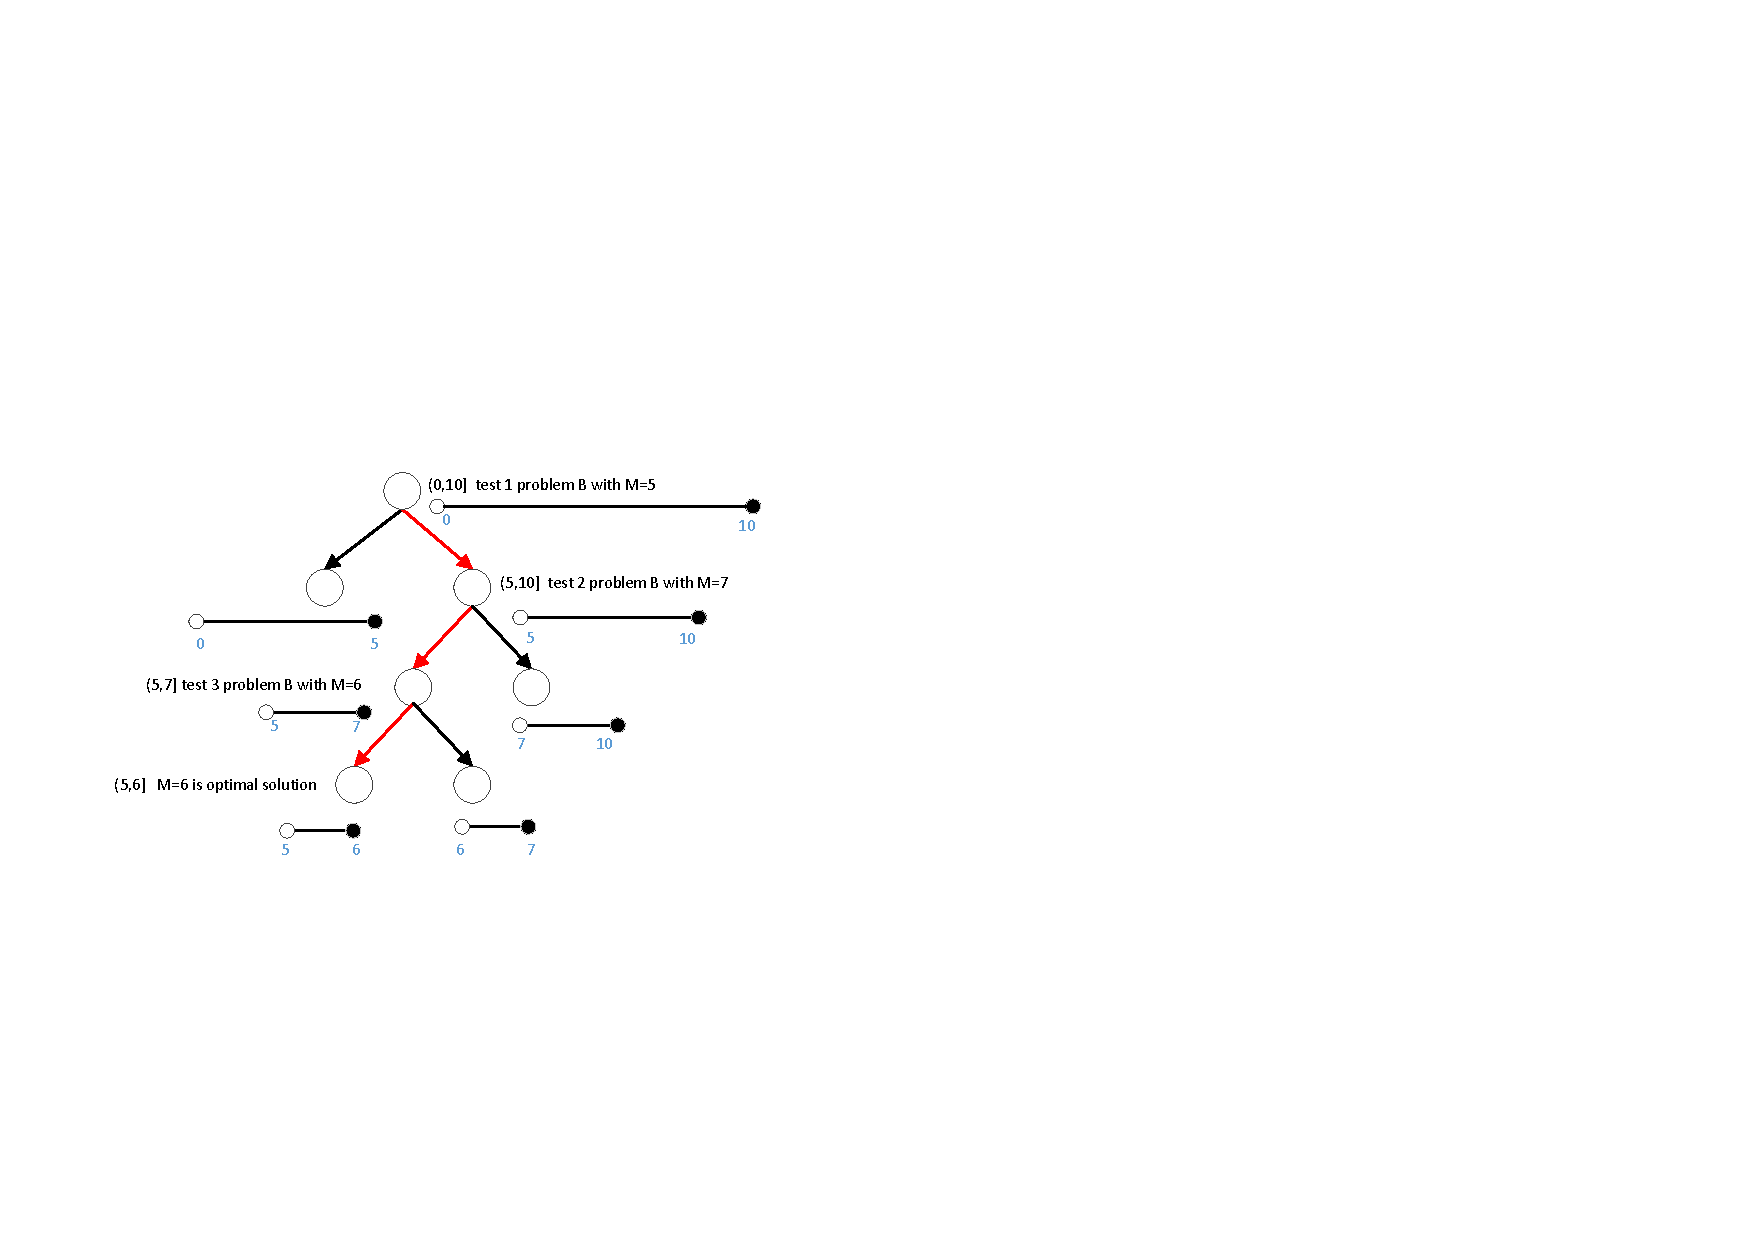
\includegraphics[width=3.0in]{figures/binarySearch}
  \caption{Request optimal solution M through Binary search method }
  \label{fig:binarySearch}
\end{figure}
假设程序X在输入问题B时,如果问题B没有解,则程序Y立即停止,否则程序B继续执行并获得问题B的解,因此问题B可以归结为NP-hard问题。因此C(B)$\leq$NP-hard。

此外,给定任意两条路径,很容易在多项式时间内判别这两条路径是否为SRLG 不相交路径,较小的路径其权重小于或等于M,从而使得C(B)$\leq$NP-complete。当B的复杂度等于A时,我们有C(A)=C(B)$\leq$NP-complete。因此,A=NP-complete。
\end{proof}
\section{陷阱问题}
基于APF的启发式算法可能会陷入“陷阱”问题。也就是说,当一个AP被确定时,即使网络中确实存在一对不相交路径对,它也可能无法找到SRLG不相交的BP路径。图.\ref{fig:CompositeGraph}.(c),(d)说明了陷阱问题。虚线表示一个AP,其链路集为$\mathbb{AP}=\{e_1,e_2,e_3$ $,e_4,e_5,e_6,e_7,e_8\}$。在删除AP上的链路和与AP共享风险的链路后,图.\ref{fig:CompositeGraph}.(d) 所示的不存在从s到d的路径,因此找不到BP。

虽然KSP算法被认为是解决陷阱问题的有效算法,但它可能面临着效率低下的问题。在这个图.\ref{fig:KSPproblem}中,假设$e_1, e_2, e_3, e_4$的链路权重比其他链路大得多。此外,在$e_1, e_2, e_3, e_4$中,$e_1$ 和$e_2$的链接权重远小于$e_3$,$e_4$。然后,在KSP算法多次找从s到d的K短路时,总是包含$e_1,e_2$(虚线表示)。则最短AP 总会遇到陷阱问题,因为$e_1$和$e_4$ 具有相同的风险,因此无法找到BP。为了避免陷阱问题,必须将K设为一个大值,这给KSP带来了很高的时间复杂度。
\begin{figure}[htbp]
\centering
% Requires \usepackage{graphicx}
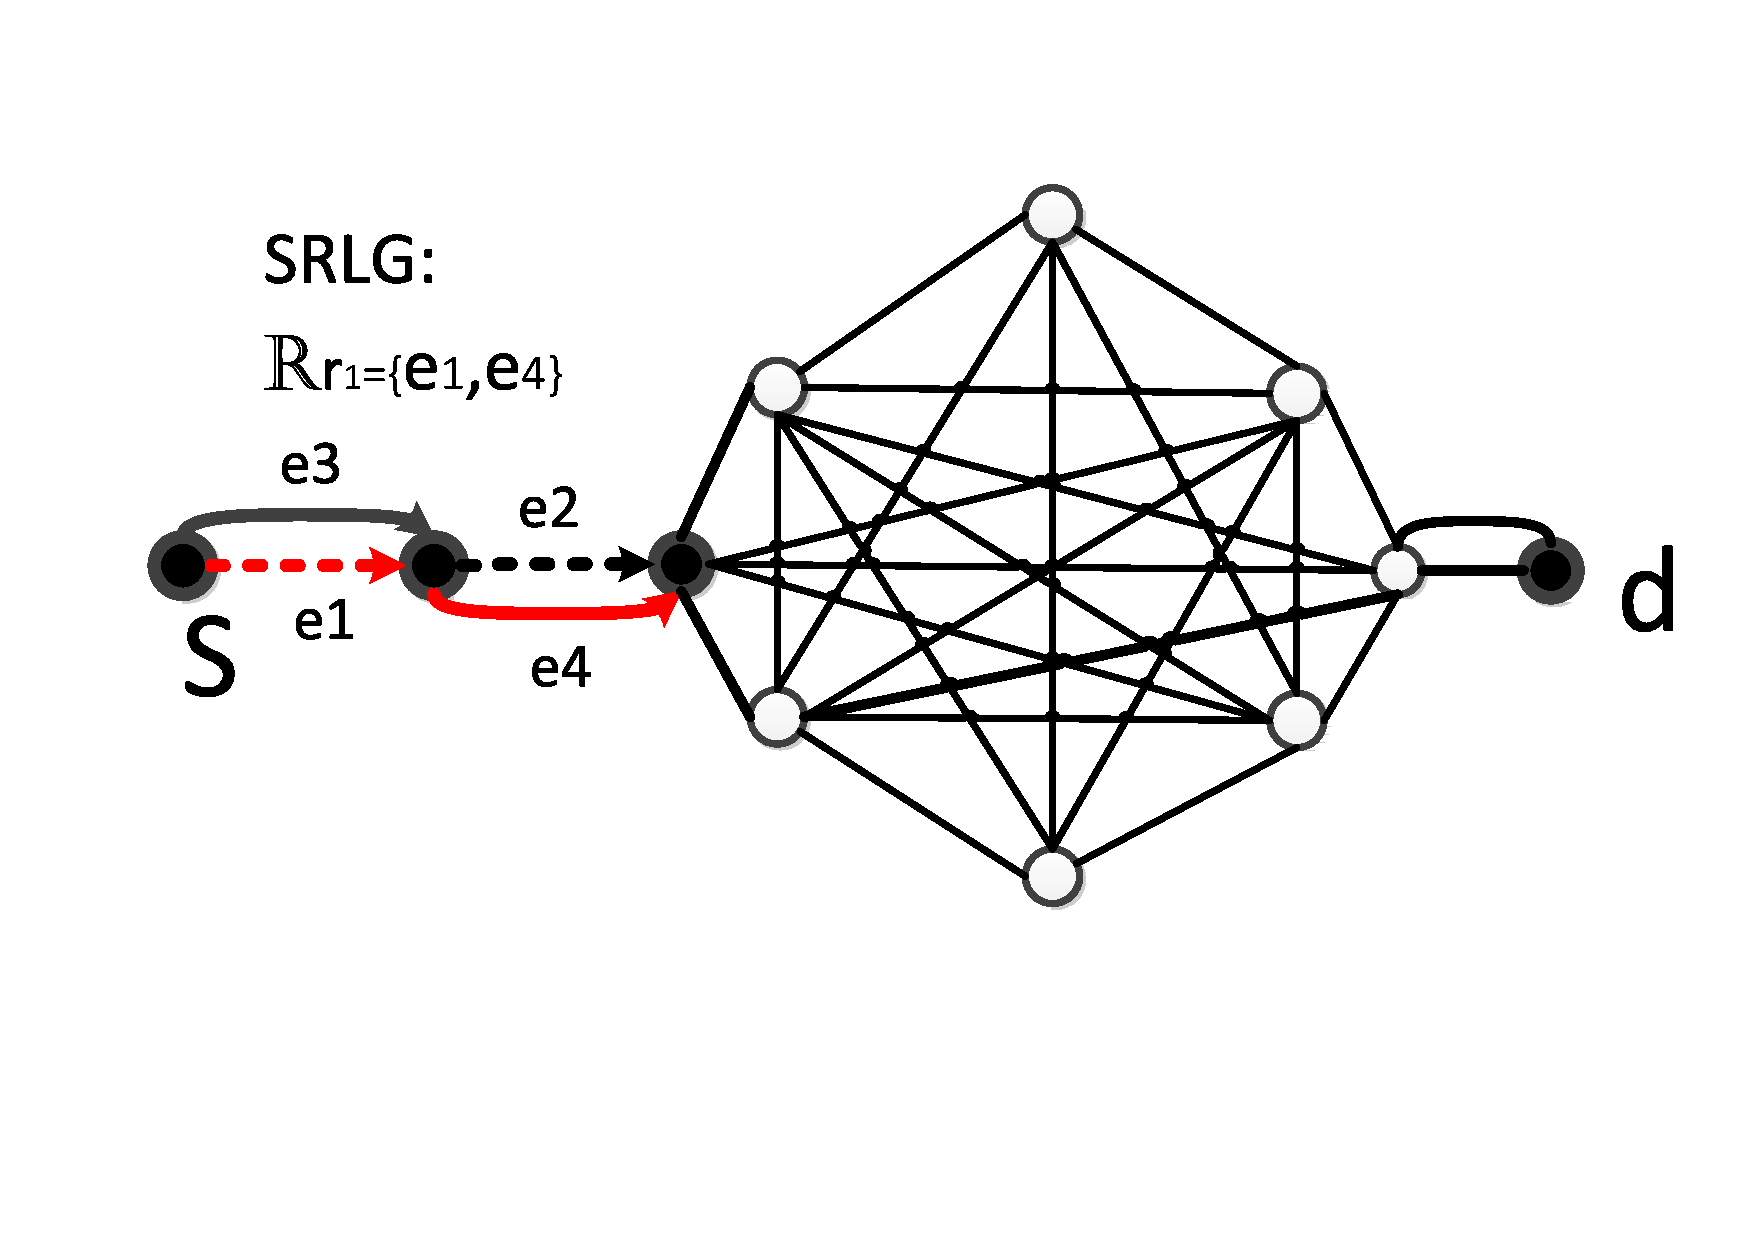
\includegraphics[width=2.8in]{figures/KSPproblem}
  \caption{An example to illustrate the inefficiency of KSP}
  \label{fig:KSPproblem}
\end{figure}


\section{分而治之的快速共享风险链路组不相交路径算法}
当一个陷阱问题发生,并且对于给定的AP没有SRLG不相交路径BP时,AP中可能存在一个子链路集,这样任何通过这个链路集里所有的这些“问题”链路的AP都不能找到一个SRLG不相交BP。 我们称之为\textbf{SRLG冲突链路集}。与KSP不同,当最短AP遇到陷阱问题时,我们将通过两个主要步骤来解决这个问题。在图.\ref{fig:KSPproblem}的例子中,我们将首先找到图.\ref{fig:KSPproblem}中的SRLG冲突链路p集合,然后应用分而治之算法将原问题划分为两个子问题$\mathcal{P}(\emptyset,\{e_1\})$和 $\mathcal{P}(\{e_1\},\{e_2\})$。 这两个子问题可以在多核CPU平台上并行执行,快速得到SRLG不相交路径对。
\subsection{分而治之}
在得到SRLG冲突链路集后,设计了一种分而治之的算法,将原Min-Min SRLG不相交路由问题划分为多个子问题,并行执行,加快求SRLG不相交路径对的过程。

为了便于问题划分,我们首先用定义两个不相交的链接集和$\mathbb{I}$和$\mathbb{O}$,其中我被称$\mathbb{I}$为包含集集合,$\mathbb{O}$称为排除集集合。由$\mathcal{P}({\mathbb{I},\mathbb{O}})$表示的Min-Min SRLG- 不相交问题,用于寻找一对AP和BP,其中AP是所有可能的AP中最短的,其中路径$AP$必须经过$\mathbb{I}$集合里的所有链路和不经过$\mathbb{O}$集合里的所有链路

最初,让$\mathbb{I}=\emptyset$ 和 ${\mathbb{O}}=\emptyset$,原来的Min-Min SRLG不相交路径对问题可以用$\mathcal{P}(\emptyset,\emptyset)$表示。给定SRLG冲突链路集$\mathbb{T}=\{{e_1},{e_2}, \cdots ,{e_{\left| \mathbb{T} \right|}}\}$,原问题$\mathcal{P}(\emptyset,\emptyset)$可按以下步骤划分。

\begin{enumerate}
  \item 首先,$\mathcal{P}(\emptyset,\emptyset)$能被划分成两个子问题$\mathcal{P}(\emptyset,\{e_1\})$ 和 $\mathcal{P}(\{e_1\},\emptyset)$。
  \item 类似,$\mathcal{P}(\emptyset,\{e_1\})$能被划分成两个子问题 $\mathcal{P}(\{e_1,e_2\},\emptyset)$ 和 $\mathcal{P}(\{e_1\},\{e_2\})$。
  \item 这个划分步骤持续直到步骤$|\mathbb{T}|$,问题$\mathcal{P}(\{e_1,e_2,\cdots ,{e_{\left| \mathbb{T} \right|-1}}\},\emptyset)$ 进一步的拆分成两个子问题$\mathcal{P}(\{e_1,e_2,\cdots ,{e_{\left| \mathbb{T} \right|-1}}, {e_{\left| \mathbb{T} \right|}}\},\emptyset)$ 和 $\mathcal{P}(\{e_1,e_2,\cdots ,{e_{\left| \mathbb{T} \right|-1}}\},{e_{\left| \mathbb{T} \right|}})$。注意到,子问题$\mathcal{P}(\{e_1,e_2,\cdots ,{e_{\left| \mathbb{T} \right|-1}}, {e_{\left| \mathbb{T} \right|}}\},\emptyset)$是无解的。
\end{enumerate}



除了子问题$\mathcal{P}(\{e_1,e_2,\cdots ,{e_{\left| \mathbb{T} \right|}}\},\emptyset)$外,我们将试图求其它每个子问题的最优解。然后选择最好的路径对(即最短路径对)。作为原问题$\mathcal{P}(\emptyset,\emptyset)$的最终(最优)解。如果这些子问题都没有解,则我们可以得出原问题没有任何解,因为我们子问题包括了所有的可能的不相交路径对。

就时间复杂性而言,解决子问题所需的时间比原来的问题应该花费的更少。因为一条链路(来自集合$\mathbb{T}$)将在计算AP的路径时被去除,这也确保了不同的AP路径将被测试且是否存在一个SRLG不相交BP路径。

当遇到陷阱问题时,我们的解决方案将划分原来的问题,并测试每个子问题以寻找到最终的解。在我们的分而治之方法中,子问题是由SRLG冲突链路集而得,而这个SRLG冲突链路集适是当AP路径遇到陷阱问题生成的。与现有的算法相比较,该算法在不考虑现有结果和问题的情况下,可以在很大程度上降低算法的计算量。对于图.\ref{fig:DividedConquer}中的例子所示,SRLG冲突链接集是$\mathbb{T}=\{e_2,e_5,e_6\}$。拆分过程过程如图.\ref{fig:DividedConquer}所示。根据SRLG冲突链路集,我们应该测试总共3个子问题${{\mathcal{P}}(\{ e_2,e_5\} ,\{ e_6\} )}$, ${{\mathcal{P}}(\{ e_2\} ,\{ e_5\} )}$ 和 ${{\mathcal{P}}(\emptyset ,\{ e_2\} )}$,其中选择AP路径权重最低的最优子问题作为原问题$\mathcal{P}(\emptyset,\emptyset)$最终的(最优)解。

注意,我们不需要解决子问题${{\mathcal{P}}(\{ e_2,e_5\}, \emptyset)}$ 和 ${{\mathcal{P}}(\{ e_2\},\emptyset )}$,因为它们的解已经包含在其它的子问题中。第一个解空间由两个子问题${{\mathcal P}(\{ e_2,e_5,e_6\} ,\emptyset )}$ 和 ${{\mathcal P}(\{ e_2,e_5\} ,\{ e_6\} )}$组成。由于SRLG冲突链接集为$\mathbb{T}=\{e_2,e_5,e_6\}$,显然,子问题${{\mathcal P}(\{ e_2,e_5,e_6\} ,\emptyset )}$是没有解的。因此,${{\mathcal P}(\{ e_2,e_5\} ,\{ e_6\} )}$的解空间等于${{\mathcal{P}}(\{ e_2, e_5\}, \emptyset)}$的解空间。同样,${{\mathcal{P}}(\{ e_2\},\emptyset )}$的解空间包括${{\mathcal{P}}(\{ e_2\} \{ e_5\}, \emptyset)}$  和 ${{\mathcal{P}}(\{ e_2\} ,\{ e_5\} )}$的解空间。
\begin{figure}[htbp]
\small{
\begin{equation*}
{\mathcal P}(\emptyset ,\emptyset )\left\{ {\begin{array}{*{20}{l}}
{{\mathcal P}(\{ e_2\} ,\emptyset )\left\{ {\begin{array}{*{20}{l}}
{{\mathcal P}(\{ e_2,e_5\} ,\emptyset )\left\{ {\begin{array}{*{20}{l}}
{{\mathcal P}(\{ e_2,e_5,e_6\} ,\emptyset )}\\
{\boxed{{\mathcal P}(\{ e_2,e_5\} ,\{ e_6\} )}}
\end{array}} \right.}\\
{\boxed{{\mathcal P}(\{ e_2\} ,\{ e_5\} )}}
\end{array}} \right.}\\
{\boxed{{\mathcal P}(\emptyset ,\{ e_2\} )}}
\end{array}} \right.
\end{equation*}
}
\caption{Example to illustrate divide-and-conquer solution}
\label{fig:DividedConquer}
\end{figure}




\subsection{SRLG冲突链路集合}
在本节中,我将描述了如何找到一个SRLG冲突链路集合,当在网络$G$中给定一个AP路径并且没有SRLG不相交的BP路径。
\subsubsection{通过新奇的边容量设置准则构造一个新的图$G^*$}
如\ref{subsubsec:maxFlow}节介绍的,如果在图G中去除所有在边割集$\mathbb{\mathbb{L}}_{\Phi}$的所有边,则$|f| = 0$。也就是说,不存在任何流能从$s$到$d$。在本文中,我们试图基于割集的概念找到SRLG冲突链路集合。如果AP从s到d流通,经过的链路与割集$\mathbb{\mathbb{L}}_{\Phi}$共享风险,则找不到任何与其对应的SRLG不相交路径BP,因为没有一条在割集中的链路可以被BP选择。

基于割集上基础上为了找到SRLG 冲突链路集,我们构造了一个新的图$G^*$ ,如下所示.
\begin{enumerate}
  \item $G^*$与$G$的节点和链路结构一样
  \item 跟每条链路$e_i$相关的链路权重$w_{e_i}$是跟其相对应图$G$中边的权重一样的。
  \item 我们使用以下准则设置每条边$e_i \in \mathbb{E}$相关的容量$c_{e_i}$
\end{enumerate}
 \begin{equation}
c_{e_i} = \left\{ {\begin{array}{*{20}{c}}
   1 & {e_i{\rm{ }} \in {\rm{ \mathbb{AP}}}}  \\
   {\left| \mathbb{AP} \right|+1} & {e_i{\rm{ }} \in {\rm{ \mathbb{E}}}{{\rm{\mathbb{R}}}}}  \\
   {\left| {{\rm\mathbb{AP}}} \right| + \left( {\left| {{\rm\mathbb{AP}}} \right| + 1} \right)\times \left| {{\rm{\mathbb{E}}}{{\rm{\mathbb{R}}}}} \right| + 1} & {otherwise}  \\
\end{array}} \right.
\label{eq:capacity principle}
\end{equation}
$\mathbb{AP}$指在图$G$中较小权重路径$AP$上所有链路的集合,和$\mathbb{\mathbb{ER}}$指不属于路径$AP$上的边但是与路径$AP$上的边共享风险的链路集合。

在图.\ref{fig:CompositeGraph}(c)所示,路径$AP$的边集合$\mathbb{AP}=\{e_1,e_2,e_3,e_4$
$,e_5,e_6,e_7,e_8\}$, $\mathbb{\mathbb{ER}}=\{e_9,e_{11},e_{17},e_{13},e_{19}\}$。$|\mathbb{AP}|=8$, $|\mathbb{\mathbb{ER}}|=5$, $|\mathbb{AP}|+1=9$ 和 ${\left| {{\rm{\mathbb{AP}}}} \right| + \left( {\left| {{\rm{\mathbb{AP}}}} \right| + 1} \right)\times \left| {{\rm{\mathbb{E}}}{{\rm{\mathbb{R}}}}} \right| + 1}=54$. 我们产生一个新图$G^*$如图.\ref{fig:FlowStarGraph}所示, 在图$G^*$中边的容量是根据公式.(\ref{eq:capacity principle})所设置.

\begin{figure}[tp]
  \centering
  % Requires \usepackage{graphicx}
  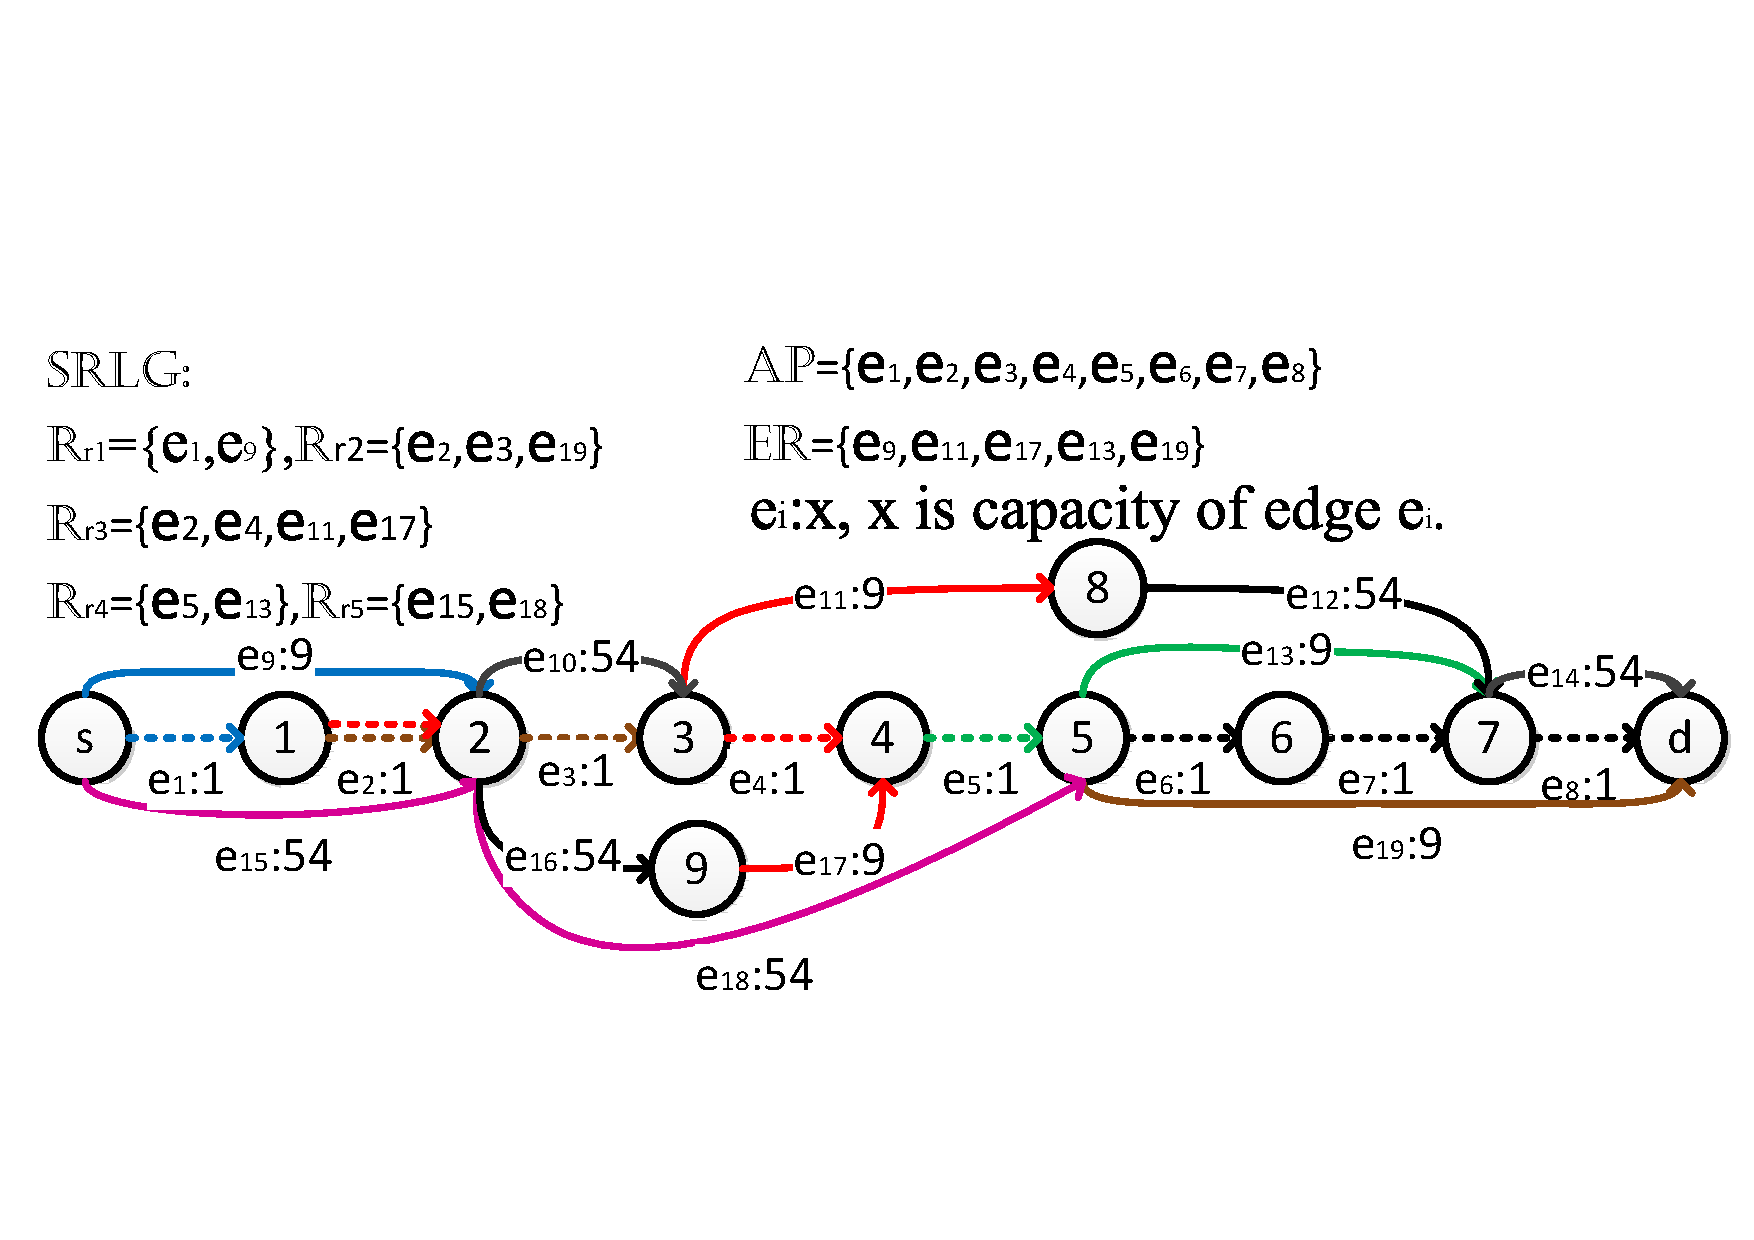
\includegraphics[width=3.6in]{figures/FlowStarGraph}
  \caption{New Graph $G^*$}\label{fig:FlowStarGraph}
\end{figure}



\subsubsection{最小割最大网络流定理}
\label{subsubsec:maxFlow}
设$G=(\mathbb{\mathbb{V}},\mathbb{\mathbb{E}})$是一个网络(其中$\mathbb{\mathbb{V}}$是$|\mathbb{\mathbb{V}}|$个节点的集合,$\mathbb{\mathbb{E}}$是$|\mathbb{\mathbb{E}}|$条链路的集合),其中$s\in \mathbb{V}$和$d\in \mathbb{V}$分别指源节点和终节点。链路$e_i$ 的\textbf{容量}表示该条链路的最大流量。链路的流$f_{e_i}$应该满足以下两个限制:
\begin{enumerate}
  \item 容量限制: $\forall e_i\in \mathbb{\mathbb{E}}$: $f_{e_i}\leq c_{e_i}$.
  \item 流量守恒: $\forall u\in \mathbb{\mathbb{V}}-\{s,d\}$: $\sum\limits_{v\in \mathbb{V}}f_{(v,u)}=\sum\limits_{v\in \mathbb{V}}f_{(u,v)}$,  $(v,u)$ 和 $(u,v)$ 代表链路 $e(v,u)$ 和 $e(u,v)$.
\end{enumerate}

流的值定义为$|f|=\sum\limits_{v\in \mathbb{V}}f_{(s,v)}$,其中s是源节点。它表示从s节点到d节点的流量。\textbf{最大流量问题}:尽可能的求从s节点到d节点的最大流量值$|f|$。

一个 s-d 割${\Phi}=(\mathbb{S},\mathbb{D})$ 是节点$\mathbb{V}$的划分满足$s \in \mathbb{S}$ 和 $d \in \mathbb{D}$。$\Phi$ 的割集合$\mathbb{\mathbb{L}}_{\Phi}$ 是一个包含边的集合。
\begin{equation}
\mathbb{\mathbb{L}}_{\Phi}=\{(u,v)\in \mathbb{E}: u \in \mathbb{S}, v \in \mathbb{D}\}.
\end{equation}

如果在割集合$\mathbb{\mathbb{L}}_{\Phi}$中的边被去除,那么在原图中的流值$|f| = 0$。即没有流能从s节点到d节点。一个 s-d 割${\Phi}=(\mathbb{S},\mathbb{D})$的容量被定义成$c(\Phi)=\sum\limits_{e_i\in \mathbb{\mathbb{L}}_{\Phi}}c_{e_i}$。\textbf{最小s-d 割 $\Phi$ 问题},最小化$c(\Phi)$即决定点集$\mathbb{S}$ 和 $\mathbb{D}$使得s-d 割${\Phi}=(\mathbb{S},\mathbb{D})$的($c(\Phi)$) 最小化 。

\textbf{最小割最大流定理}:一个s-d流的最大值等于s-d割的最小割。如图.\ref{fig:FlowNetwork}所示,在图$G$中的流量$|f|=f_{(s,v_1)}+f_{(s,v_2)}$。这个割$\Phi(\mathbb{S},\mathbb{D})$ 是 $\mathbb{S}=\{s,v_1,v_2,v_4\}$ 和$\mathbb{D}=\{v_3,d\}$,它是最小的割其容量为$c(\Phi)=c_{(v_1,v_3)}+c_{(v_4,v_3)}+c_{(v_4,d)}=12+7+4=23$. 显然, $|f|=c(\Phi)$, 即s-d 最大流等于所有s-d割中最小的容量。
\begin{figure}[htbp]
  \centering
  % Requires \usepackage{graphicx}
  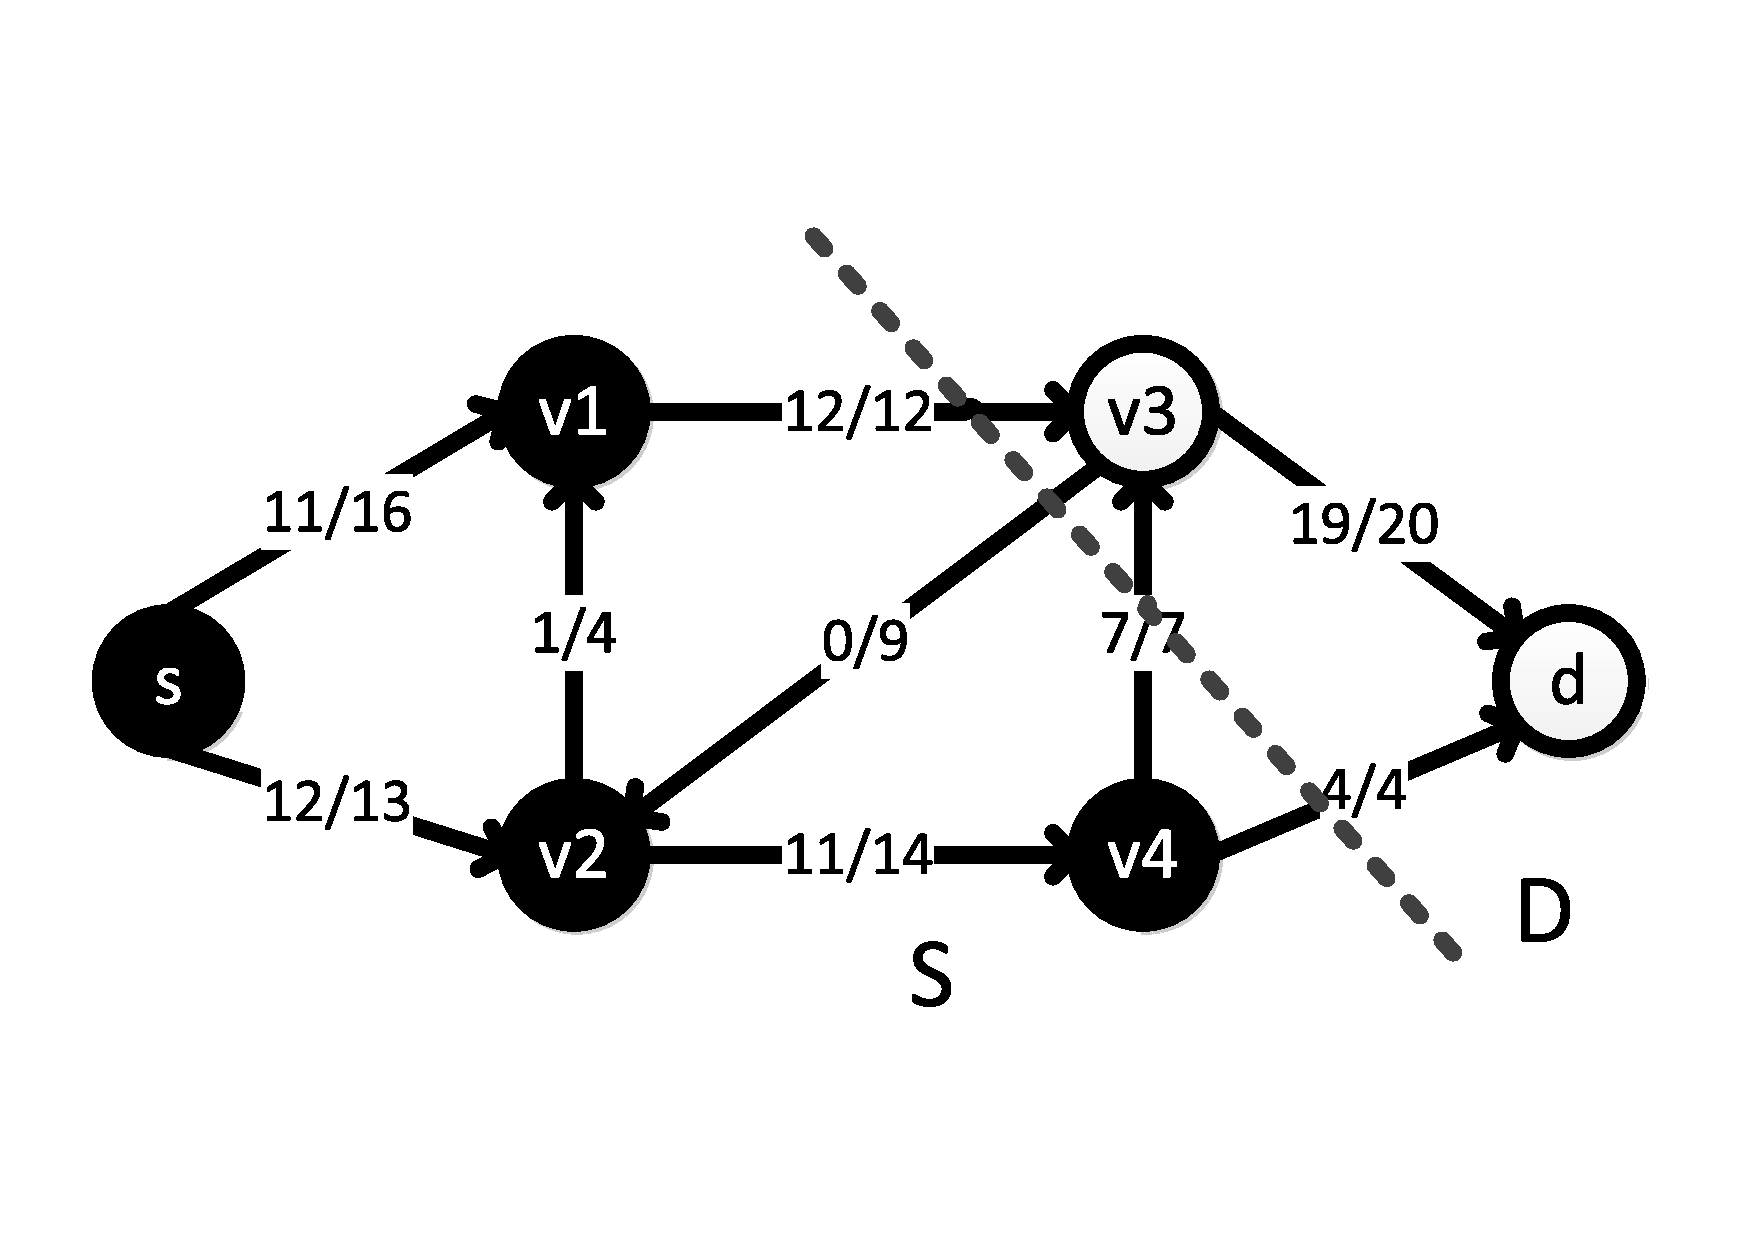
\includegraphics[width=2.5in]{figures/FlowNetwork}\\
  \caption{An example to illustrate max-flow min-cut theorem. Each link $e_i$ is labeled by $f_{e_i}/c_{e_i}$, where $f_{e_i}$ and $c_{e_i}$ denote the flow and capacity of link $e_i$, respectively.   }
  \label{fig:FlowNetwork}
\end{figure}

\subsubsection{新图$G^*$中最小割集的性质}
最大流最小割定理指出,在网络中,从源节点$s$到目的节点$d$最大流值等于最小边割集的总容量,即最小的链路总容量,如果删除最小边割集上的边,将断开目的节点$d$与源节点$s$的连通。 我们的算法基于图的最小割集的链路集来求得最小SRLG 冲突链路集。

我们将首先展示我们重建新图$G^*$的一些优良特性为求得最小SRLG冲突链路集。

\begin{lemma}
\label{le:lemma1}
    在图$G^*$任何从$s$到$d$的路径必须经过一条边在边集合 $\mathbb{AP}$ 或者 $\mathbb{\mathbb{ER}}$中。
    %note:draw a picture to describe the proof
\end{lemma}
\begin{proof}
我们用矛盾的方法证明这条引理。假设对于某条路径AP,有另一条路径从$s$到$d$在图$G^*$中不与AP共享风险,即这条路径不通过$\mathbb{AP}$ 或者 $\mathbb{\mathbb{ER}}$的任何一条链路。我们可以很容易得出这样的结论,这条路径是与路径AP对应的SRLG不相交路径BP。这与AP没有对应的SRLG不相交路径的说法相矛盾。
\end{proof}

\begin{lemma}
\label{le:lemma2}
    图$G^*$的任何一条最大流的流值是最多为$|\mathbb{AP}|+(|\mathbb{AP}|+1)\times|\mathbb{\mathbb{ER}}|$。
\end{lemma}
\begin{proof}
假设$G^*$的最大流f为$|f|=k$。在$G^*$中,f可以被划分为k个从s到d的1单元流。根据引理.\ref{le:lemma1},这些1单位流中的每一个都必须通过通过$\mathbb{AP}$ 或者 $\mathbb{\mathbb{ER}}$的至少一个链路。请注意,$\mathbb{AP}$ 或者 $\mathbb{\mathbb{ER}}$ 中链路的容量分别为1或者$|\mathbb{AP}|$+1。根据$\mathbb{AP}$ 和 $\mathbb{\mathbb{ER}}$中链路的容量设置,因为$\mathbb{AP}$中的链路只能承载1单位流量,而在ER中,一条链路在$\mathbb{ER}$中能最多承载$|\mathbb{AP}|$+1单位流量.因此,最多只能有$|\mathbb{AP}|+ (|\mathbb{AP}|+1)\times|\mathbb{\mathbb{ER}}|$个从s到d的单位流量。
\end{proof}

\begin{lemma}
\label{le:lemma3}
    图$G^*$的最小割$\Phi$的边割集$\mathbb{L}_{\Phi}$所有链路都在$\mathbb{AP}$ 或者$\mathbb{\mathbb{ER}}$中。
\end{lemma}

\begin{proof}
根据最大流最小切定理,$c(\Phi)$表示的最小切割$\Phi$的的容量,其应该等于最大流量值,根据引理 \ref{le:lemma2}最大流量最多为$|\mathbb{AP}|+ |\mathbb{ER}|\times (|\mathbb{AP}|+1)$。 根据容量设定原则如公式\ref{eq:capacity principle}所示,一条链路既不在$\mathbb{AP}$ 也不在 $\mathbb{ER}$ ($e_i \notin \mathbb{AP}$ 和 $e_i \notin \mathbb{ER}$), 这条链路的容量为 $c_{e_i} = \left| {{\rm\mathbb{AP}}} \right| + \left( {\left| {{\rm\mathbb{AP}}} \right| + 1} \right)\times \left| {{\rm{\mathbb{E}}}{{\rm{\mathbb{R}}}}} \right| + 1$, 这条链路是大于$|\mathbb{AP}|+(|\mathbb{AP}|+1)\times |\mathbb{ER}|$. 因此,这条链路不可能在$\mathbb{L}_{\Phi}$中. 因此,割集$\mathbb{L}_{\Phi}$中的所有链路都必须属于边集合$\mathbb{AP}$ 或者 $\mathbb{ER}$。
\end{proof}


\begin{theorem}
    如果在图$G$中一个单元流阻塞了全部边割集$\mathbb{L}_{\Phi}$的所有边,则在原图中不会存在任何流经过这个图的割。
\label{th:block flow}
\end{theorem}


\begin{proof}
    如果在图$G$中一个单元流阻塞了全部边割集$\mathbb{L}_{\Phi}$的所有边,则在原图中没有流能使用边割集$\mathbb{L}_{\Phi}$ 里的边和没有任何流能经过这个图的割。
\end{proof}
定理\ref{th:block flow}提供了找到SRLG冲突链路集的可能性。即当AP路径遇到陷阱问题时,我们找到$\mathbb{AP}$路径边集的子集能够阻塞国有在边割集$\mathbb{L}_{\Phi}$的所有边,和这个子集即SRLG冲突链路集。当一条路径包含SRLG冲突链路集里的所有边,则没有任何流能经过割集$\Phi$,因此没有与其对应的SRLG不相交路径BP。

\subsubsection{SRLG冲突链路集的集合覆盖问题}
虽然AP路径上的所有链接一起构成了SRLG冲突链路集,我们感兴趣的是尽量规模较小的SRLG冲突链路集,SRLG冲突链路集的大小确定不相交成的子问题规模。

根据定理\ref{th:block flow},最小SRLG冲突链路集问题可以描述为:查找AP 链路集上的最小链路子集,这些链路可以阻塞边割集$\mathbb{L}_{\Phi}$。

对于任何链路$e_i$,$\mathbb{SR}_{e_i}$表示与链路$e_i$共享风险的链接集。显然,$\mathbb{SR}_{e_i}$包括$e_i$本身和所有包含链路$e_i$风险贡献链路组SRLG集合的所有边。例如,如图\ref{fig:MinCutStarGraph}所示,$e_i$ 是在两个SRLG中$\mathbb{R}_{r_2}=\{e_2,e_3,e_{19}\}$, $\mathbb{R}_{r_3}=\{e_2,e_4,e_{11},e_{17}\}$,因此, $\mathbb{SR}_{e_2}=\{e_2,e_3,e_{19},e_4,e_{11},e_{17}\}$。

对每条在AP上的路径$e_i$,我们定义每条边的cut-block-link集合为${\mathbb{B}_{{e_i}}} = \mathbb{SR}_{{e_i}} \cap \mathbb{L}_{\Phi}$,这个集合是边割集$\mathbb{L}_{\Phi}$的子集,能通过$e_i$而堵塞这个集合的所有边。

因此,最小SRLG冲突链路集问题可以定义为一个集合覆盖问题:给定$\mathbb{AP}$(路径AP上的链路集合)、边割集$\mathbb{L}_{\Phi}$和cut-block-link集合${\mathbb{B}_{{e_1}}},{\mathbb{B}_{{e_2}}}, \cdots ,{\mathbb{B}_{{e_{|\mathbb{AP}|}}}}$。我们求出最小cut-block-link集合集,其交集是边割集$\mathbb{L}_{\Phi}$,即最小规模的$\mathbb{T} \subseteq \{e_i| e_i\in \mathbb{AP}\}$ 以至于 ${ \cup_{e_i \in \mathbb{T}}}{\mathbb{B}_{e_i}} = \mathbb{L}_{\Phi}$。


\begin{figure*}[htbp]
  \centering
  % Requires \usepackage{graphicx}
  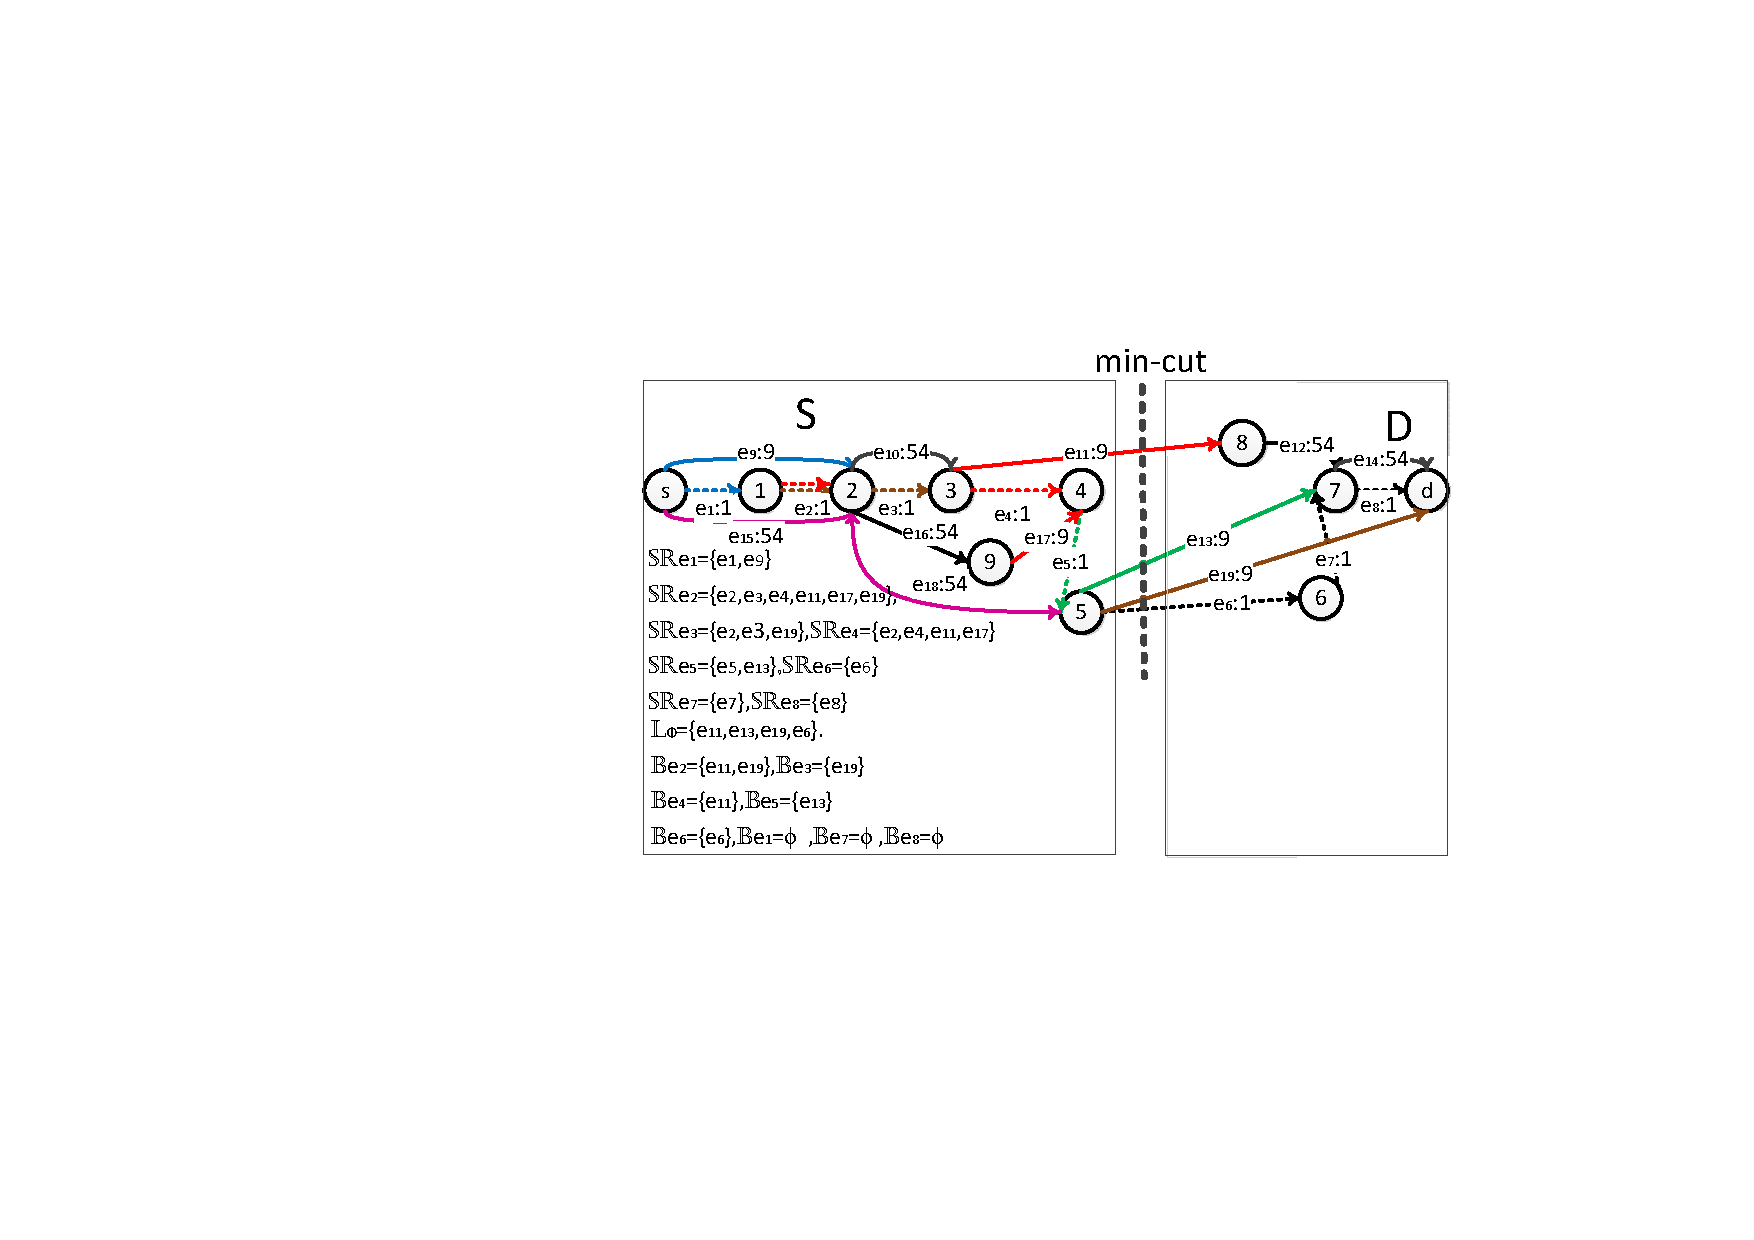
\includegraphics[width=3.8in]{figures/MinCutStarGraph}
  \caption{Min cut of the network graph, $\mathbb{SR}_{e_1}=\{e_1, e_9\},\mathbb{SR}_{e_2}=\{e_2,e_3,e_4, e_{11},e_{17},e_{19}\},\mathbb{SR}_{e_3}=\{e_2,e_3, e_{19}\},\mathbb{SR}_{e_4}=\{e_2,e_4, e_{11},e_{17}\},\mathbb{SR}_{e_5}=\{e_5, e_{13}\},\mathbb{SR}_{e_6}=\{e_6\},\mathbb{SR}_{e_7}=\{e_7\} $ and $\mathbb{SR}_{e_8}=\{e_8\}$. $\mathbb{L}_{\Phi}=\{e_{11},e_{13},e_{19},e_{6}\}$. $\mathbb{B}_{e_1}=\emptyset,\mathbb{B}_{e_2}=\{e_{11},e_{19}\},\mathbb{B}_{e_3}=\{e_{19}\},\mathbb{B}_{e_4}=\{e_{11}\},\mathbb{B}_{e_5}=\{e_{13}\},\mathbb{B}_{e_6}=\{e_6\}$,$\mathbb{B}_{e_7}=\emptyset$ and $\mathbb{B}_{e_8}=\emptyset$.}\label{fig:MinCutStarGraph}
  \label{fig:MinCutStarGraph}
\end{figure*}

集合覆盖问题通常是一个np-hard问题。它的复杂性取决于元素的大小(表示($N$)。在我们的最小SRLG冲突链路集问题中,$n=|\mathbb{L}_{\Phi}|$,即割集$\mathbb{L}_{\Phi}$的边数。因为本文的重点不是改进集合覆盖问题算法,我们应用\cite{chvatal1979greedy}中提出的算法。在复杂度$O(log(|\mathbb{L}_{\Phi}|))$的情况下求出最小的SRLG冲突链路集,通常即使是在大规模的网络,最短的路径作为AP都没有大跳数$n=|\mathbb{L}_{\Phi}|$。因此,用集合覆盖问题来求最小值SRLG冲突链路集代价不是很大。

为了说明如何找到最小SRLG冲突链路集,我们如图\ref{fig:MinCutStarGraph}所展示了一个例子。为了求最小$\Phi(\mathbb{S},\mathbb{D})$, $\mathbb{S}=\{s, 1, 2, 3, 4, 5, 9\}$和$\mathbb{D}=\{d, 6, 7, 8\}$。边割集$\mathbb{L}_{\Phi}=\{e_{11},e_{13},e_{19},e_{6}\}$。对于AP路径上的所有链路,cut-block-link集合是:$\mathbb{B}_{e_1}=\emptyset$, $\mathbb{B}_{e_2}=\{e_{11},e_{19}\}$, $\mathbb{B}_{e_3}=\{e_{19}\}$, $\mathbb{B}_{e_4}=\{e_{11}\}$, $\mathbb{B}_{e_5}=\{e_{13}\}$, $\mathbb{B}_{e_6}=\{e_6\}$, $\mathbb{B}_{e_7}=\emptyset$ and $\mathbb{B}_{e_8}=\emptyset$。为了覆盖$\mathbb{L}_{\Phi}$,最少的cut-block-link集合是$\mathbb{B}_{e_6}=\{e_6\}$, $\mathbb{B}_{e_7}=\emptyset$ and $\mathbb{B}_{e_8}=\emptyset$。因此,最小SRLG冲突链路集是$\mathbb{T}=\{e_2, e_5, e_6 \}$。

如图\ref{fig:MinCutStarGraph}所示的例子中,虽然$|\mathbb{L}_{\Phi}|=4$,但是最小SRLG冲突链路集$|\mathbb{T}|=|\{e_2, e_5, e_6 \}|=3$是小于$|\mathbb{L}_{\Phi}|=4$。这是因为$e_2$属于$\mathbb{R}_{r_2}$和$\mathbb{R}_{r_3}$,并能阻塞在割集$\mathbb{L}_{\Phi}$中的两条链路$e_{11}$和$e_{19}$


根据SRLG的拓扑类型\cite{datta2008graph},SRLG的拓扑类型:星型类型和非星型类型。对星型类型SRLG,所有链路都从同一个节点开始或结束在同一个节点。例如,如图\ref{fig:MinCutStarGraph}所示,$e_1$和$e_9$来自相同的节点$s$,$\mathbb{R}_{r_1}$是星型SRLG。对非星型类型,并不是SRLG中的所有链路都是从相同节点开始或结束于同一节点。如图\ref{fig:MinCutStarGraph}所示,$\mathbb{R}_{r_2}$, $\mathbb{R}_{r_3}$, $\mathbb{R}_{r_4}$ 和 $\mathbb{R}_{r_5}$是非星型类型。而且,即使在图\ref{fig:MinCutStarGraph}所示包括星型SRLG 和无星型SRLG,我们的算法高效且有效地通过解决集合覆盖问题来解决冲突集。


因此,与现有的一些研究不同的是,\cite{datta2008graph}只能处理单个SRLG类型,这样的简单场景中一条链路只属于一个SRLG,我们的算法能更有效的处理多种情形。在更一般的情况下,链路可以属于一个或多个SRLG具有更多不同的SRLG类型。



\subsection{时间复杂度}
在为了查找SRLG不相交路径对时,当AP遇到陷阱问题,我们的算法首先计算出SRLG冲突链路集,然后通过把原问题划分成T个子问题来求解原问题。如\ref{subsec:Set cover problem for SRLG Conflicting Link Set}节所述边割集$\mathbb{L}_{\Phi}$的边数规模通常不是很大,因此,本算法寻找SRLG冲突链路集不会带来太多的时间成本。因此,我们关注的是路径查找过程的计算开销。

一般来说,对于一个有$|\mathbb{E}|$条链路和$|\mathbb{V}|$个节点的网络,求最小权重路径问题的复杂性是$(|\mathbb{E}|+|\mathbb{V}|)\times log(|\mathbb{V}|)$。为了解决陷阱问题,我们的路径查找问题与最初的最小权重路径问题有点不同。我们在路径查找的过程中引入了一些约束条件。例如,查找AP路径必须通过必过链路集和必不过链路集。由于这些链路集通常并不大,这些约束在成本计算上几乎没有差别。因为不同的子问题有不同的链路集,为了使描述简单明了,我们仍然使用$(|\mathbb{E}|+|\mathbb{V}|)\times log(|\mathbb{V}|)$作为一次路径搜索时间复杂度。而我们算法将原问题分成$|\mathbb{T}|$个子问题,算法复杂度为$|\mathbb{T}|\times(|\mathbb{E}|+|\mathbb{V}|)\times log(|\mathbb{V}|)$。


对于不同算法复杂性的比较,我们也展示了在Cose\cite{rostami2007cose}和KSP\cite{eppstein1998finding}在路径查找过程中的复杂性。

CoSE试图找到一个冲突的SRLG集合,而不是一个冲突链路集。但是他们寻找冲突的SRLG集的方法是穷尽的查找而且成本很高。在这我们主要分析研究路径查找过程时间成本。由于我们的SRLG冲突链路集是由最小割和集合覆盖问题导出的,$|\mathbb{T}|$是最小的SRLG冲突链路集规模。因此,在CoSE中的冲突SRLG集至少是$|\mathbb{T}|$,并且我们表示SRLG集合为$\left\{ {SRL{G_1},SRL{G_2}, \cdots ,SRL{G_{|\mathbb{T}|}}} \right\}$,由于每个SRLG路径包含多条链路,因此CoSE的子问题应该比我们的要大得多。在AP路径上的一个SRLG 的必过链路集合不过链路集会产生$|SRLG|$个子问题。所以一个SRLG集合$\left\{ {SRL{G_1},SRL{G_2}, \cdots ,SRL{G_{|\mathbb{T}|}}} \right\}$将引入$\prod\limits_{i = 1}^{_{\left| T \right|}} {\left| {SRL{G_i}} \right|}$个子问题。因此CoSE的复杂性是$\prod\limits_{i = 1}^{_{|\mathbb{T}|}} {\left| {SRL{G_i}} \right|}\times (|\mathbb{E}|+|\mathbb{V}|)\times log(|\mathbb{V}|)$,这是比我们的算法那复杂度大得多的。

对于KSP算法\cite{eppstein1998finding},路径查找复杂度为$K\times ((|\mathbb{E}|+|\mathbb{V}|)\times log(|\mathbb{V}|))$,其中K是在发现SRLG不相交路径对之前应该测试的路径次数。然而,由于KSP没有从前面的路径搜索过程利用前面的信息,在最坏的情况下,KSP可能尝试从源节点$s$到目的节点$d$的所有路径。因此,最糟糕的K值是$2^{|\mathbb{E}|}$,这会带来很大的计算成本。


\section{实验环境与评价指标}

因为我们找不到任何拓扑带有SRLG链路属性,所以我们通过注入SRLG信息生成一个合成的数据集。拓扑数据有$\TopoNum$种不同的拓扑,具有不同的节点数目、链路数目、链路权重(表示链路的延迟或其他参数),如表\ref{tab:AllSample}所示显示了拓扑的基本属性。这7个拓扑中的节点、链路)。

\begin{table*}[htbp]
\caption{SRLG拓扑数据}
  \centering
\footnotesize{  \begin{tabular}{*{18}{c}}
\toprule
拓扑 & 1 & 2 & 3 & 4 & 5 & 6& 7   \\
\midrule
点   &     527&      521    &      521     &    2023             &     451     &     521     &     449       \\
边   &    4158 &  4052     &    4152      &   4142          &       2780   &      4052   &      2778    \\
%Graph density  & 1.5\% &    1.49\% &   1.52\%  &  0.1\%  &   0.10\% &   1.41\%  &  1.5\% &   1.38\%   \\
No.SRLG & 132 &  86   &  89  &  207        & 210  &  128  &   88    \\
SRLG边比率 & 9.66\% & 6.16\% &   6.18\% &   14.94\%    &   22.55\%  &  9.65\% &   9.53\%     \\
\bottomrule
\end{tabular}
}
\label{tab:AllSample}
\end{table*}

为了进行性能比较,除了我们的算法(名为\CI),我们还实现了另外四个SRLG不相交路径对算法。算法如下:
\begin{enumerate}
  \item ILP:\cite{hu2003diverse} 中的工作旨在寻找SRLG不相交路径对。通过整数线性规划方程使这两条路径总的权重最小化。我们没有找到其他通过整数线性规划方程寻找Min-Min SRLG不相交路径对的方法的研究。因此,从\cite{hu2003diverse}的整数规划方程,通过改变目标函数构造Min-Min SRLG 不相交路径对问题的整数线性规划方程。
  \item IQCP:因为任意0−-1整数线性规划方程,其中所有变量为0或1,原问题的整数线性规划方程可以表示为一个二次约束方程,我们还设计了Min-Min SRLG 不相交路径问题成一个整数二次约束规划(IQCP)\cite{hu2003diverse}。
  \item KSP\cite{eppstein1998finding}:它在源节点$s$和目的节点$d$中找到第K短路作为候选AP路径,一个接一个地测试候选的AP路径是否有相应的SRLG不相交路径BP,直到我们发现了这样的BP,算法才结束。
  \item CoSE\cite{rostami2007cose}:当AP遇到陷阱问题时,CoSE尝试进行简单而详尽的搜索,以找到一个SRLG集合。任何AP路径通过这个SRLG集都无法找到SRLG不相交的BP路径。基于这个SRLG集合,它划分原问题并设计算法来求SRLG不相交路径对。
\end{enumerate}


前两者(ILP和IQCP)是基于整数规划模型的。在我们的实现中,工具GUROBI 7.0\cite{optimization2012gurobi}用于解决这两个整数规划问题。六种性能指标用于评估不同的SRLG分路径算法:
\begin{itemize}
  \item 路径权重:路径中链路权重的总和。
  \item 路径跳数:路径中的跳数。
  \item 运行时间:查找SRLG不相交路径对的归一化平均时间。
  \item 算法加速比:给定两种不同的算法($alg_1$ 和$alg_2$)的计算时间,表示为$T_1$ 和 $T_2$,算法$alg_1$对于算法$alg_2$计算时间上的加速比是$alg_1$: ${S_{1 - 2}} = T_1/T_2$。
  \item 核加速比:并行程序的核心加速比\cite{grama2003introduction}通常定义为$S_P=\frac{T_1}{T_p}$,其中p是处理器内核和$T_1$和$T_p$表示在1核和$p$核上的运行时间。
  \item 效率\cite{grama2003introduction}:定义为$E_p=\frac{S_p}{p}=\frac{T_1}{pT_p}$,它是百分比(0,1)的范围内。


\end{itemize}


所有实现都是在linux服务器上运行的,这个服务器配置Intel(R) Xeon(R) CPU E5-2620  2.00GHz(24 核)和32.00GB内存。为了测量计算时间,我们在所有实现的算法中插入一个定时器。

我们通过在拓扑数据集里注入SRLG链路属性产生了两种SRLG类型,星型类型和非星型类型。在光纤网络中,SRLG是星型类型,而在其他网络类型中,例如一个Overlay网络中,SRLG可以是非星型的。每个SRLG组是通过随机选择2-5链路组成的。在五种SRLG不相交路径对算法中,只有CoSE和我们SCLS是并行算法。尽管ILP、IQCP和KSP不是并行算法,我们仍然在实现它们来体现出我算法设计所获得的速度增益,归一化\cite{tax2000feature}所有拓扑数据的结果为最终结果。


\section{算法性能评估及比较}
从\ref{subsec:Complexity analysis}节分析,在KSP下求第一条$K$最短路的计算复杂度是$2^{|\mathbb{E}|}\times ((|\mathbb{E}|+|\mathbb{V}|)\times log(|\mathbb{V}|))$,最坏的情况下这将是$K\times ((|\mathbb{E}|+|\mathbb{V}|)\times log(|\mathbb{V}|))$。与分析一致,当我们使用7个拓扑运行KSP,没有仿真结果能在1 小时内返回,而其他算法则可以在11 秒内。计算时间长使得KSP难以在实践中使用。因此,我们不在结果显示KSP。
\begin{enumerate}
  \item 路径权重:如图\ref{fig:normalization weitgh sum}所示,显示AP路径权重、BP路径权重和AP和BP的总和路径权重。显然,所有的算法SCLS、CoSE、ILP和IQCP实现了相同的AP路径权重。但是不同的算法有不同的BP权重,因此它们有不同的路径权重和。因为所有算法都解决了SRLG不相交路径对问题,尽管他们发现不同的SRLG不相交路径对,它们都能达到找到最小权重相等的AP路径。然而,这两个基于整数线性规划的算法,ILP 和IQCP,主要是找到最小化AP的权重但是其随意找到其它任何SRLG不相交路径BP,因此这两个算法搜索到的BP路径是不同的。
  \item 路径跳数:图\ref{fig:normalization weitgh sum}显示AP路径跳数、BP路径跳数和AP和BP路径跳数之和,因为所有算法的目标都是最小化SRLG不相交路径对的最小路径权重。在路径跳数中,它们具有相同的AP权重(如图\ref{fig:normalization weitgh sum}所示)但是他们有不同的AP路径跳数(如图\ref{fig:normalization hop} 所示)。尽管所有算法的AP路径权重都小于BP路径权重如图\ref{fig:normalization weitgh sum}所示,在图\ref{fig:normalization hop}中,AP跳数可能并不总是少于BP路径跳数。
  \item 运行时间:如图\ref{fig:normalization runtime}所示,通过改变使用的CPU核数来展示不同算法下的运行时间。由于CoSE下的运行时明显大于其他算法的运行时,为了更清楚地展示其他算法的结果,我们在图\ref{fig:Runtime_noKSP_noCOSE} 中通过排除CoSE来进一步绘制运行时间的结果。由于ILP和IQCP不是并行算法,这些算法在不同核数下的运行时间大致相等。我们的SCLS和CoSE的运行时间随着处理器核数的增加而减少,因为这两种算法可以将原问题划分为多个子问题来并行执行,并利用多核CPU的并行性来加快路径搜索的速度,虽然CoSE是一种并行算法,但计算时间比ILP和IQCP 还要大。一些可能的原因包括:1)在CoSE中冲突SRLG集合的搜索过程效率不高;2)由于一个SRLG 通常包含多条链路,基于冲突SRLG问题的划分将带来大量的子问题需要解决,这也将带来大量的计算量。与CoSE不同的是,当AP上遇到陷阱问题时我们的SCLS根据图中的最小割集理论来求SRLG冲突链路集,并达到图\ref{fig:normalization runtime}中所示的最低时间消耗。这说明了我们的冲突链路集查找算法是有效的,并且我们提出的分治算法和基于SRLG冲突链路集的智能AP搜索过程,可以大大降低计算量。
   \item   算法加速比:如图\ref{fig:Multiple}所示,我们进一步比较了它们的计算速度。特别地,为了找出使用不同算法寻找所需路径时所获得的加速比,我们使用CoSE作为基准算法,并设置$alg_1$ =CoSE。与图\ref{fig:normalization runtime}中的结果相似,在图\ref{fig:Multiple} 中SCLS的加速度是CoSE的1000倍以上。在图\ref{fig:Multiple} 中由于CoSE的运行速度明显小于其他算法,很难在图\ref{fig:Multiple}中观察到,我们在图\ref{fig:MultipleNoSCLS}中排除了最大的SCLS数据来进一步绘制了算法加速比结果。
   \item 核加速比:与使用算法加速比来比较所有算法的总体运行速度不同,这个度量“核加速比”是来评估CPU中的核数如何影响给定算法的运行速度。图\ref{fig:Speedup}绘制了所有实现的算法的核加速比。算法ILP和IQCP下的核加速比在任意核数下近似等于1,因为它们不是并行算法。当核数小于4时,我们的SCLS的核心加速比随着核数的增加而增加,当超过4核时,SCLS的核心加速比保持稳定,说明4核对SCLS是足够的。这一结果与Amdahl定律\cite{amdahl1967validity}是一致的,即理论核加速比确定的上界限定于问题的规模大小。但是,即使核心数等于8,CoSE下的核加速比也继续增加,这是数字4的两倍。结果表明,即使是8核CPU也不能满足COSE的并行性要求.这是因为CoSE发现的冲突SRLG集包含了大量的链路,这进一步导致了大量的子问题,从而导致了较大的问题规模和计算成本。
    \item 效率:与图\ref{fig:Speedup}相似,随着更多的核增多效率值会降低,因为一个大的核心数会带来更多的成本来协调进程。如图\ref{fig:Efficiency}所示,所有算法的效率值都随着核心数的增加而降低。与图\ref{fig:Speedup}中的结果一致,由于CoSE引入的子问题比我们的SCLS多,在核心数达到4之后,CoSE下的效率大于SCLS。然而,如图\ref{fig:Multiple}所示我们的SCLS实现了更大的算法加速比。
\end{enumerate}

全部仿真结果表明,在搜索速度较快的情况下,SCLS算法的性能优于其他算法,因为我们算法发现的冲突链路集可以方便有效的执行并行算法并且计算量小。

\begin{figure}[htbp]
\centering
\begin{minipage}[t]{0.45\linewidth}
\centering
\includegraphics[width=2.25in]{figures/weight}
\caption{路径权重}
\label{fig:normalization weitgh sum}
\end{minipage}
\hfill
\begin{minipage}[t]{0.45\linewidth}
\centering
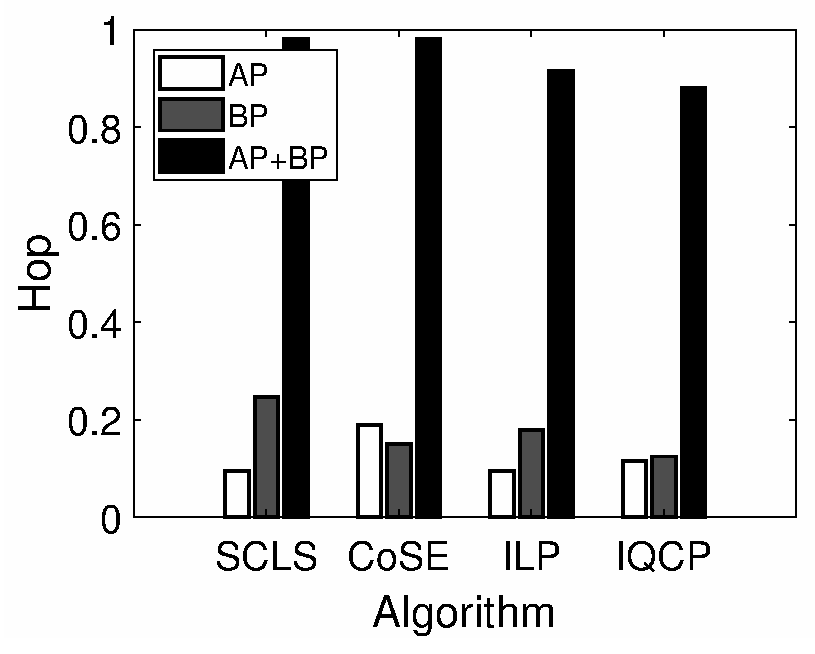
\includegraphics[width=2.25in]{figures/hop}
\caption{路径跳数}
\label{fig:normalization hop}
\end{minipage}
\end{figure}


\begin{figure*}[htbp]
\centering
\begin{minipage}[t]{0.3\linewidth}
\centering
\includegraphics[width=2.25in]{figures/runtime}
\caption{运行时间}
\label{fig:normalization runtime}
\end{minipage}
\hfill
\begin{minipage}[t]{0.3\linewidth}
\centering
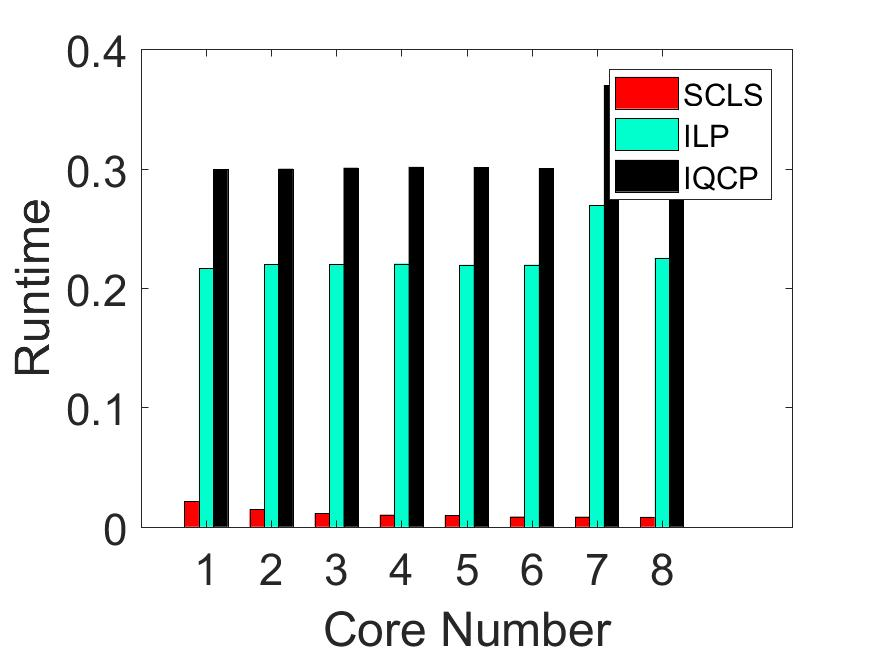
\includegraphics[width=2.25in]{figures/Runtime_noKSP_noCOSE}\\
  \caption{运行时间(无CoSE)}\label{fig:Runtime_noKSP_noCOSE}
\end{minipage}
\hfill
\begin{minipage}[t]{0.3\linewidth}
\centering
\includegraphics[width=2.25in]{figures/speedup}
\caption{核加速比}
\label{fig:Speedup}
\end{minipage}
\end{figure*}


\begin{figure*}[htbp]
\centering
\begin{minipage}[t]{0.3\linewidth}
\centering
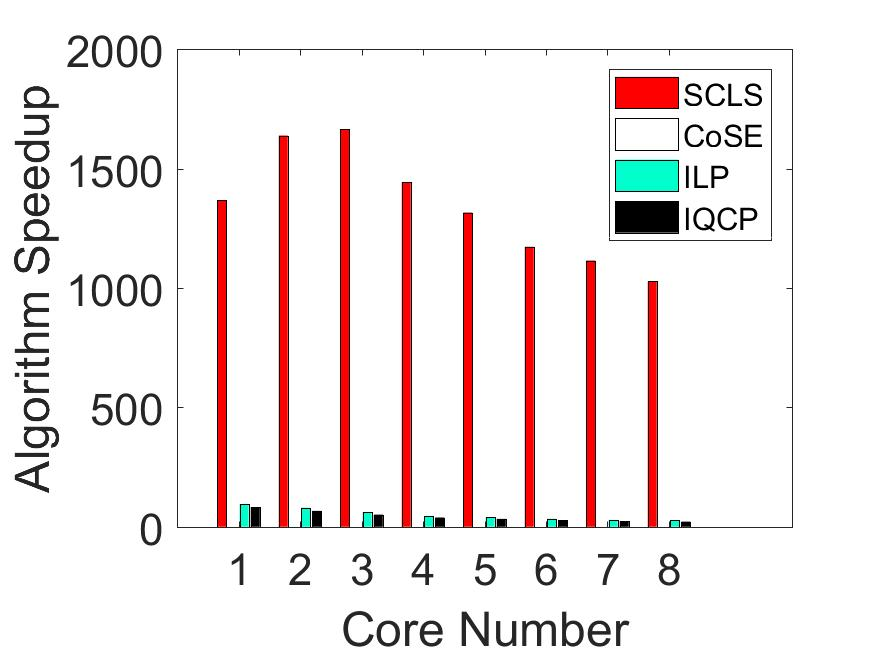
\includegraphics[width=2.25in]{figures/Multiple}
\caption{算法加速比}
\label{fig:Multiple}
\end{minipage}
\hfill
\begin{minipage}[t]{0.3\linewidth}
\centering
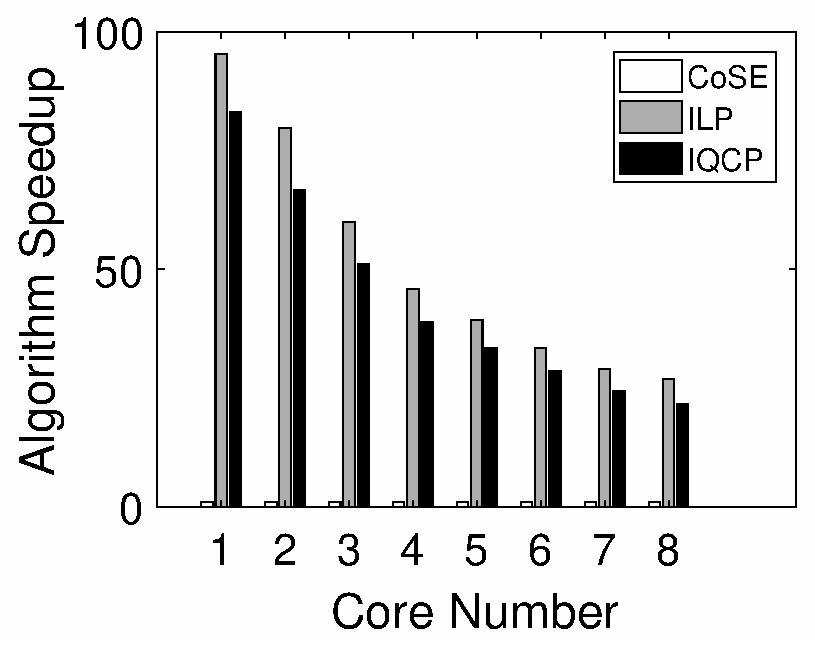
\includegraphics[width=2.25in]{figures/MultipleNoSCLS}
\caption{算法加速比(无SCLS)}
\label{fig:MultipleNoSCLS}
\end{minipage}
\hfill
\begin{minipage}[t]{0.3\linewidth}
\centering
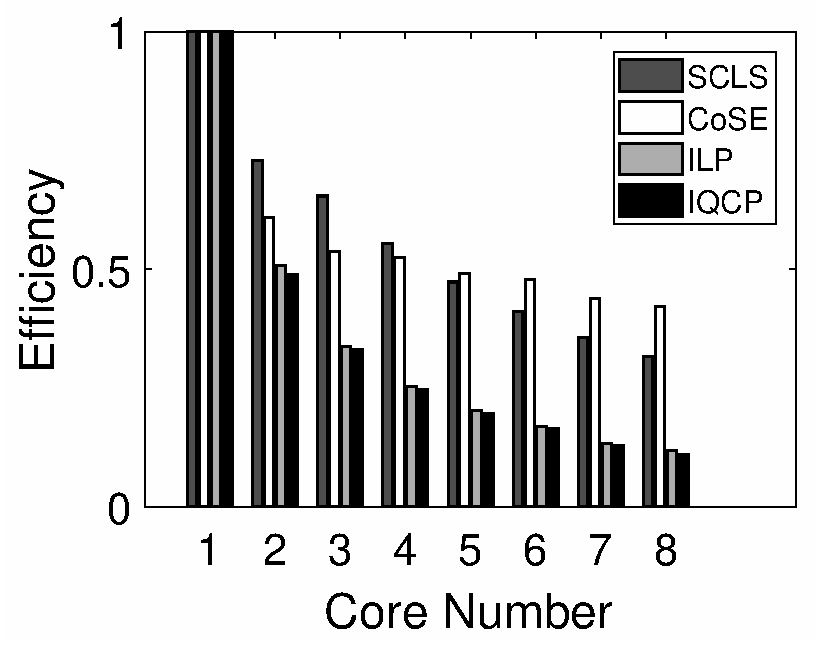
\includegraphics[width=2.25in]{figures/Efficiency}
 \caption{效率}
 \label{fig:Efficiency}
\end{minipage}
\end{figure*}





%\chapter{可生存性虚拟网络映射算法研究}
\section{面向底层单节点失效的}
\section{算法性能评估}
\section{本章小节}

%\chapter{总结和展望}
\section{本文工作总结}
\section{未来研究工作与展望}
p


%% !Mode:: "TeX:UTF-8"

\chapter{模板介绍与注意事项}
\section{模板说明}

HNUThesis~是为了帮助湖南大学毕业生撰写毕业论文而编写的~\LaTeX~论文模板,其前提是用户已经能处理一般的~\LaTeX~文档,并对~BibTeX~有一定了解,如果你从来没有接触过~\LaTeX~,建议先学习相关基础知识,磨刀不误砍柴工,能有助你更好使用模板。

由于个人水平有限,虽然现在的这个版本基本上满足了学校的要求,但难免存在不足之处,欢迎大家积极反馈,更希望湖南大学~\LaTeX~爱好者能一同完善此模板,让更多同学受益。

如有模板的疑问或有意向加入模板的维护和编写队伍中来,请给作者: franztaoheng@gmail.com(陶恒)写信。

\section{下载安装}
HNUThesis~主页:~\url{http://hnuthesis.googlecode.com/}。除此之外,不再维护任何镜像。

\section{目录内容}
本~\LaTeX{}~模板的源文件即为研究生毕业设计论文中使用的模板,用户可以通过修改这些文件来编辑自己的毕业论文。
\begin{itemize}
\item{hnumain.tex}:主文件,包含封面部分和其他章节的引用信息。
\item{preface}: 包含本科毕业设计论文的封面和中英文摘要。
\item{body}: 包含本文正文中的所有章节。
\begin{itemize}
\item{intros.tex}: 包括本~\LaTeX{}~模板的介绍,编译方法和使用方法。
\item{figures.tex}: 包含论文中图片的插入和引用方法。
\item{tables.tex}: 包含论文中表格的插入和引用方法。
\item{equations.tex}: 包含论文中数学符号、公式的书写和排版方法。
\item{others.tex}: 包含论文中使用的罗列环境,定理环境等其他环境的排版方法。
\item{conclusion.tex}: 包含本文的总结。
\end{itemize}
\item{setup}:存放论文所使用的宏包和全文格式的定义。
\item{appendix}:存放作者的发表论文和参加科研情况说明以及致谢文件。
\item{references/reference.bib}:存放论文所引用的全部参考文献信息。
\item{clean.bat}:双击此文件,可以用来清理~hnumain.tex~在编译之后生成的所有附属文件,如后缀名为~.aux~,~.log~,~.bak~的文件。
\end{itemize}

需要说明的是,以上文件名并不是固定的,各位同学可以新建一个~tex~文件,例如~algorithm.tex,放在~body~目录下,并且在~hnumain.tex~中调用:
\begin{verbatim}
    \include{body/algorithm.tex}
\end{verbatim}
来引用之。当然你也可以重命名这些文件,只要~include~中的文件名是存在且合法,~\LaTeX~总能找到这些文件的。

在你写作某一章节的时候,你可能需要随时预览排版效果并~Debug,这时你可以在其他章节的\verb|\include|命令前加上一个\%,这代表注释掉本行,例如:
\begin{verbatim}
%%%%%%%%%%%%%%%%%%%%%%%%%%%%%%%%
           正文部分
%%%%%%%%%%%%%%%%%%%%%%%%%%%%%%%%
\mainmatter
% !Mode:: "TeX:UTF-8"

\chapter{模板介绍与注意事项}
\section{模板说明}

HNUThesis~是为了帮助湖南大学毕业生撰写毕业论文而编写的~\LaTeX~论文模板,其前提是用户已经能处理一般的~\LaTeX~文档,并对~BibTeX~有一定了解,如果你从来没有接触过~\LaTeX~,建议先学习相关基础知识,磨刀不误砍柴工,能有助你更好使用模板。

由于个人水平有限,虽然现在的这个版本基本上满足了学校的要求,但难免存在不足之处,欢迎大家积极反馈,更希望湖南大学~\LaTeX~爱好者能一同完善此模板,让更多同学受益。

如有模板的疑问或有意向加入模板的维护和编写队伍中来,请给作者: franztaoheng@gmail.com(陶恒)写信。

\section{下载安装}
HNUThesis~主页:~\url{http://hnuthesis.googlecode.com/}。除此之外,不再维护任何镜像。

\section{目录内容}
本~\LaTeX{}~模板的源文件即为研究生毕业设计论文中使用的模板,用户可以通过修改这些文件来编辑自己的毕业论文。
\begin{itemize}
\item{hnumain.tex}:主文件,包含封面部分和其他章节的引用信息。
\item{preface}: 包含本科毕业设计论文的封面和中英文摘要。
\item{body}: 包含本文正文中的所有章节。
\begin{itemize}
\item{intros.tex}: 包括本~\LaTeX{}~模板的介绍,编译方法和使用方法。
\item{figures.tex}: 包含论文中图片的插入和引用方法。
\item{tables.tex}: 包含论文中表格的插入和引用方法。
\item{equations.tex}: 包含论文中数学符号、公式的书写和排版方法。
\item{others.tex}: 包含论文中使用的罗列环境,定理环境等其他环境的排版方法。
\item{conclusion.tex}: 包含本文的总结。
\end{itemize}
\item{setup}:存放论文所使用的宏包和全文格式的定义。
\item{appendix}:存放作者的发表论文和参加科研情况说明以及致谢文件。
\item{references/reference.bib}:存放论文所引用的全部参考文献信息。
\item{clean.bat}:双击此文件,可以用来清理~hnumain.tex~在编译之后生成的所有附属文件,如后缀名为~.aux~,~.log~,~.bak~的文件。
\end{itemize}

需要说明的是,以上文件名并不是固定的,各位同学可以新建一个~tex~文件,例如~algorithm.tex,放在~body~目录下,并且在~hnumain.tex~中调用:
\begin{verbatim}
    \include{body/algorithm.tex}
\end{verbatim}
来引用之。当然你也可以重命名这些文件,只要~include~中的文件名是存在且合法,~\LaTeX~总能找到这些文件的。

在你写作某一章节的时候,你可能需要随时预览排版效果并~Debug,这时你可以在其他章节的\verb|\include|命令前加上一个\%,这代表注释掉本行,例如:
\begin{verbatim}
%%%%%%%%%%%%%%%%%%%%%%%%%%%%%%%%
           正文部分
%%%%%%%%%%%%%%%%%%%%%%%%%%%%%%%%
\mainmatter
% !Mode:: "TeX:UTF-8"

\chapter{模板介绍与注意事项}
\section{模板说明}

HNUThesis~是为了帮助湖南大学毕业生撰写毕业论文而编写的~\LaTeX~论文模板,其前提是用户已经能处理一般的~\LaTeX~文档,并对~BibTeX~有一定了解,如果你从来没有接触过~\LaTeX~,建议先学习相关基础知识,磨刀不误砍柴工,能有助你更好使用模板。

由于个人水平有限,虽然现在的这个版本基本上满足了学校的要求,但难免存在不足之处,欢迎大家积极反馈,更希望湖南大学~\LaTeX~爱好者能一同完善此模板,让更多同学受益。

如有模板的疑问或有意向加入模板的维护和编写队伍中来,请给作者: franztaoheng@gmail.com(陶恒)写信。

\section{下载安装}
HNUThesis~主页:~\url{http://hnuthesis.googlecode.com/}。除此之外,不再维护任何镜像。

\section{目录内容}
本~\LaTeX{}~模板的源文件即为研究生毕业设计论文中使用的模板,用户可以通过修改这些文件来编辑自己的毕业论文。
\begin{itemize}
\item{hnumain.tex}:主文件,包含封面部分和其他章节的引用信息。
\item{preface}: 包含本科毕业设计论文的封面和中英文摘要。
\item{body}: 包含本文正文中的所有章节。
\begin{itemize}
\item{intros.tex}: 包括本~\LaTeX{}~模板的介绍,编译方法和使用方法。
\item{figures.tex}: 包含论文中图片的插入和引用方法。
\item{tables.tex}: 包含论文中表格的插入和引用方法。
\item{equations.tex}: 包含论文中数学符号、公式的书写和排版方法。
\item{others.tex}: 包含论文中使用的罗列环境,定理环境等其他环境的排版方法。
\item{conclusion.tex}: 包含本文的总结。
\end{itemize}
\item{setup}:存放论文所使用的宏包和全文格式的定义。
\item{appendix}:存放作者的发表论文和参加科研情况说明以及致谢文件。
\item{references/reference.bib}:存放论文所引用的全部参考文献信息。
\item{clean.bat}:双击此文件,可以用来清理~hnumain.tex~在编译之后生成的所有附属文件,如后缀名为~.aux~,~.log~,~.bak~的文件。
\end{itemize}

需要说明的是,以上文件名并不是固定的,各位同学可以新建一个~tex~文件,例如~algorithm.tex,放在~body~目录下,并且在~hnumain.tex~中调用:
\begin{verbatim}
    \include{body/algorithm.tex}
\end{verbatim}
来引用之。当然你也可以重命名这些文件,只要~include~中的文件名是存在且合法,~\LaTeX~总能找到这些文件的。

在你写作某一章节的时候,你可能需要随时预览排版效果并~Debug,这时你可以在其他章节的\verb|\include|命令前加上一个\%,这代表注释掉本行,例如:
\begin{verbatim}
%%%%%%%%%%%%%%%%%%%%%%%%%%%%%%%%
           正文部分
%%%%%%%%%%%%%%%%%%%%%%%%%%%%%%%%
\mainmatter
\include{body/intros}
%%\include{body/figures}
%%\include{body/tables}
%%\include{body/equations}
%%\include{body/others}
%%\include{body/conclusion}
\end{verbatim}
那么,编译的时候就只编译未加~\%~的一章,在这个例子中,即本章~intros。

理论上,并不一定要把每章放在不同的文件中。但是这种自顶向下,分章节写作、编译的方法有利于提高效率,大大减少~Debug~过程中的编译时间,同时减小风险。

\section{参考文献生成方法}

\LaTeX~具有插入参考文献的能力。Google Scholar~网站上存在兼容~BibTeX~的参考文献信息,通过以下几个步骤,可以轻松完成参考文献的生成。
\begin{itemize}
  \item 在\href{http://scholar.google.com/}{谷歌学术搜索}中,
        点击\href{http://scholar.google.com/scholar_preferences?hl=en&as_sdt=0,5}{学术搜索设置}。
  \item 页面打开之后,在\textbf{文献管理软件}选项中选择\textbf{显示导入~BibTeX~的链接},单击保存设置,退出。
  \item 在谷歌学术搜索中检索到文献后,在文献条目区域单击导入~BibTeX~选项,页面中出现文献的引用信息。
  \item 将文献引用信息的内容复制之后,添加到~references~文件夹下的~reference.bib~中。
\end{itemize}

\section{编译注意事项}
\begin{enumerate}
  \item 由于模板使用~UTF-8~编码,所以源文件应该保存成~UTF-8~格式,否则可能出现中文字符无法识别的错误。
  本模板中每一个~.tex~文件的文件的开头已经加上一行:\\
    \verb|% !Mode:: "TeX:UTF-8"|\\
     这样可以确保~.tex~文件默认使用~UTF-8~的格式打开。读者如果删去此行,很有可能会导致中文字符显示乱码。
     在~WinEdt~编辑器中可以使用以下两种方式保存成~UTF-8~格式:
      \begin{enumerate}
        \item 先建立~.tex~文件,另存为~.tex~文件时,选择用~UTF-8~格式保存。
        \item
            在~WinEdt~编辑器中,选择\\
            \mbox{~Document$\to$Document Settings$\to$Document Mode $\to$TeX:UTF-8} 同时在~WinEdt~最下面的状态栏中,可以看到该文档是~TeX~格式还是~TeX:UTF-8~格式。
            当文档为~TeX:UTF-8~格式时,状态栏一般显示:
            \makebox[\textwidth][l]{Wrap | Indent | INS | LINE |Spell | TeX:UTF-8 | -src~等。}
      \end{enumerate}
  \item 如果在pdf书签中,中文显示乱码的话,则注意以下说明:
    \begin{verbatim}
        \usepackage{CJKutf8}
        % 1. 如果使用CJKutf8
        %    Hyperref中应使用unicode参数
        % 2. 如果使用CJK
        %    Hyperref则使用CJKbookmarks参数
        %    可惜得到的PDF书签是乱码,建议弃用
        % 3. Unicode选项和CJKbookmarks不能同时使用
        \usepackage[
        %CJKbookmarks=true,
        unicode=true
        ]{hyperref}
     \end{verbatim}
 \item 建议采用以下两种编译方式:
  \begin{enumerate}
     \item latex + bibtex + latex + latex + dvi2pdf. 在这种编译情况下,对应的~hnumain.tex~文件的第一行是\verb|\def\usewhat{dvipdfmx}|~(缺省设置)。 此时,所有图片文件应该保存为~.eps~格式,如~figures~文件夹里~.eps~图片。
          如果您选择在命令行中操作,可以在编译的时候依次输入~latex hnumain, bibtex hnumain, latex hnumain, latex hnumain~和~dvipdfmx hnumain, 编译完成之后,需要手动打开~pdf~文件。
     \item pdflatex + pdflatex. 在这种编译情况下,对应的~hnumain.tex~文件的第一行应该改为\verb|\def\usewhat{pdflatex}|~。 此时, 编译不支持~.eps~图片格式,此时需要在命令行下使用~epstopdf~指令将~figures~文件夹下 的~.eps~文件转化成~.pdf~文件格式,命令行中操作格式为~epstopdf a.eps~。
          在命令行编译的时候,依次输入~pdflatex hnumain~和~pdflatex hnumain, 编译完成之后,需要手动打开~pdf~文件。
  \end{enumerate}
\end{enumerate}

\section{系统要求}
    CTEX 2.8, MiKTeX 2.8, TeX Live 2009~或以上版本。使用推荐的~WinEdt 6.0~编辑器,可以完成文件的编辑和编译工作。

\section{\TeX~简介}

以下内容是~milksea@bbs.ctex.org~撰写的关于~\TeX~的简单介绍,略有改动。
注意这不是一个入门教程,不讲~\TeX~系统的配置安装,也不讲具体的~\LaTeX~代码。
这里仅仅试图以一些只言片语来解释:
进入这个门槛之前新手应该知道的注意事项,以及遇到问题以后该去如何解决问题。

\subsection{什么是 \TeX/\LaTeX,我是否应该选择它~?}

\TeX~是最早由高德纳(Donald Knuth)教授创建的一门标记式宏语言,
用来排版科技文章,尤其擅长处理复杂的数学公式。\TeX~同时也是处理这一语言的排版软件。
\LaTeX~是 Leslie Lamport 在~\TeX~基础上按内容/格式分离和模块化等思想建立的一集~\TeX~上的格式。

\TeX~本身的领域是专业排版领域
但现在~TeX/LaTeX~也被广泛用于生成电子文档甚至幻灯片等,~\TeX~语言的数学部分
偶尔也在其他一些地方使用。但注意~\TeX~并不适用于文书处理(Microsoft Office 的领域,以前和现在都不是)。

选择使用~\TeX/\LaTeX~的理由包括:
\begin{itemize}
\item 免费软件;
\item 专业的排版效果;
\item 是事实上的专业数学排版标准;
\item 广泛的西文期刊接收甚或只接收 LaTeX 格式的投稿;
\item[] ……
\end{itemize}
不选择使用~\TeX/\LaTeX~的理由包括:
\begin{itemize}
\item 需要相当精力学习;
\item 图文混合排版能力不够强;
\item 仅在数学、物理、计算机等领域流行;
\item 中文期刊的支持较差;
\item[] ……
\end{itemize}

请尽量清醒看待网上经常见到的关于~\TeX~与其他软件的优劣比较和口水战。在选择使用或离开之前,请先考虑
\TeX~的应用领域,想想它是否适合你的需要。


\subsection{我该用什么编辑器~?}

编辑器功能有简有繁,特色不一,从简单的纯文本编辑器到繁复的 Emacs,因人而易。基本功能有语法高亮、方便编译预览就很好了,扩充功能和定制有无限的可能。初学者可以使用功能简单、使用方便的专用编辑器,如 ~TeXWorks、Kile、WinEdt~等,或者类似所见即所得功能的~LyX;熟悉的人可以使用定制性更强的~Notepad++、SciTE、Vim、Emacs ~等。这方面的介绍很多,一开始不妨多试几种,找到最适合自己的才是最好的。

另外提醒一句,编辑器只是工作的助手,不必把它看得太重。

\subsection{我应该看什么~\LaTeX~读物~?}

这不是一个容易回答的问题,因为有许多选择,也同样有许多不合适的选择。
这里只是选出一个比较好的答案。更多更详细的介绍可以在版面和网上寻找(注意时效)。

近两年~\TeX~的中文处理发展很快,目前没有哪本书在中文处理方面给出一个最新进展的合适综述,
因而下面的介绍也不主要考虑中文处理。

\begin{enumerate}

\item 我能阅读英文。
\begin{enumerate}
\item 迅速入门:ltxprimer.pdf (LaTeX Tutorials: A Primer, India TUG)
\item 系统学习:A Guide to LaTeX, 4th Edition, Addison-Wesley
               有机械工业出版社的影印版(《\LaTeX{}~实用教程》)
\item 深入学习:要读许多书和文档,TeXbook 是必读的
\item 细节学习:去读你使用的每一个宏包的说明文档
\item 专题学习:阅读讲数学公式、图形、表格、字体等的专题文档
\end{enumerate}

\item 我更愿意阅读中文。
\begin{enumerate}
\item 迅速入门:lnotes.pdf (LaTeX Notes, 1.20, Alpha Huang)
\item 系统学习:《\LaTeXe{}~科技排版指南》,邓建松(电子版)
      如果不好找,可以阅读《\LaTeXe~入门与提高》第二版,陈志杰等,或者 《\LaTeXe~完全学习手册》,胡伟
\item 深入学习:~TeXbook0.pdf~(特可爱原本,TeXbook 的中译,xianxian)
\item 具体问题释疑:~CTeX-FAQ.pdf~,\\
        吴凌云,~\url{http://www.ctex.org/CTeXFAQ}~
\end{enumerate}
\end{enumerate}

遇见问题和解决问题的过程可以快速提高自己的技能,建议此时:
\begin{itemize}
  \item 利用~Google~搜索。
  \item 清楚,扼要地提出你的问题。
\end{itemize}

\subsection{什么知识会过时~?什么不会~?}

\TeX~是排版语言,也是广泛使用的软件,并且不断在发展中;
因此,总有一些东西会很快过时。作为学习~\TeX~的人,
免不了要看各种各样的书籍、电子文档和网络论坛上的只言片语,
因此了解什么知识会迅速过时,什么知识不会是十分重要的。

最稳定的是关于~Primitive \TeX~和~Plain \TeX~的知识,也就是 Knuth
在他的《The TeXbook》中介绍的内容。因为~\TeX~
系统开发的初衷就是稳定性,要求今天的文档到很久以后仍可以得到完全相同的结果,
因此 Knuth 限定了他的~\TeX~语言和相关实现的命令、语法。这些内容许多年来就没有多少变化,
在未来的一些年里也不会有什么变化。
Primitive \TeX~和 Plain \TeX~的知识主要包括 \TeX~排版的基本算法和原理,
盒子的原理,底层的 \TeX~命令等。其中技巧性的东西大多在宏包设计中,
初学者一般不会接触到很多;而基本原理则是常常被提到的,
譬如,~\TeX~把一切排版内容作为盒子(box)处理。

相对稳定的是关于基本~\LaTeXe~
的知识,也包括围绕~\LaTeXe~的一些核心宏包的知识。~\LaTeXe~
是自~1993~年以来的一个稳定的~\LaTeX~版本,直到最近的一次修订
(2005 年)都没有大的变动。
\LaTeX~的下一个计划中的版本~\LaTeX 3~遥遥无期,在可预见的将来,~\LaTeXe~不会过时。
\LaTeXe~的知识是目前大部分~\LaTeX~书籍的主体内容。关于~\LaTeX~的标准文档类
~(article、report、book、letter、slide~等),关于基本数学公式的输入,
文档的章节层次,表格和矩阵,图表浮动体,LR 盒子与段落盒子……
这些~\LaTeX~的核心内容都是最常用的,相对稳定的。
与~\LaTeXe~相匹配的核心宏包,
如~graphics(x)、ifthen、fontenc、doc~等,也同样是相对稳定的。
还有一些被非常广泛应用的宏包,如~amsmath~系列,也可以看作是相对稳定的。

简单地说,关于基本~\TeX/\LaTeX~的语言,都是比较稳定的。与之对应,实现或者支持~\TeX/\LaTeX~语言的软件,
包括在~\TeX/\LaTeX~基础上建立的新的宏,都不大稳定。

容易过时的是关于第三方~\LaTeX~宏包的知识、第三方~\TeX~工具的知识,以及新兴~\TeX~相关软件的知识等。
~\TeX~和~\LaTeX~语言是追求稳定的;但无论是宏包还是工具,作为不断更新软件,它们是不稳定的。
容易过时的技术很多,而且现在广泛地出现在几乎所有~\LaTeX~文档之中,因此需要特别引起注意:
宏包的过时的原因可能是宏包本身的升级换代带来了新功能或不兼容,
也可能是同一功能的更新更好的宏包代替了旧的宏包。前者的典型例子比如绘图宏包~PGF/TikZ~,
现在的~2.00~版功能十分强大,和旧的~1.1x~版相差很大,和更旧的~0.x~版本则几乎完全不同;后
者的典型例子比如~caption~宏包先是被更新的~caption2~宏包代替,后来~caption~宏包更新又使得
caption2 宏包完全过时。——安装更新的发行版可以避免使用过旧的宏包;
认真阅读宏包自带的文档而不是搜索得到的陈旧片断可以避免采用过时的代码。

工具过时的主要原因也是升级换代和被其他工具替换。前者的典型例子是编辑器
WinEdt~在~5.5~以后的版本支持~UTF-8~编码,而旧版本不支持;
后者的典型例子是中文字体安装工具从~GBKFonts~到~xGBKFonts~到~FontsGen~不断被取代。
图形插入是一个在~\TeX~实现、宏包与外围工具方面都更新很快的东西。
在过去,最常用的输出格式是~PS(PostScript)~格式,因此插入的图像以~EPS~为主流。
使用~Dvips~为主要输出工具,外围工具有~GhostScript、bmeps~等等,相关宏包有~graphics~等,
相关文档如《\LaTeXe{}~ 插图指南》。

但凡提及“~\LaTeX~只支持~EPS~图形”的,就是这个过时的时代的产物。事实上~\TeX/\LaTeX~
并不限定任何图形格式,只不过是当时的输出格式(PS)和工具(Dvips)对~EPS~情有独钟而已。
后来 PDF 格式成为主流。~pdf\TeX、DVIPDFM、DVIPDFMx、XeTeX~工具则主要支持~PDF、PNG、JPG~格式的图形,
涉及一系列工具如~ImageMagick、ebb~等。

值得特别提出注意的就是,中文处理也一起是更新迅速、容易过时的部分。
而且因为中文处理一直没有一个“官方”的“标准”做法,软件、工具、
文档以及网上纷繁的笔记也就显得相当混乱。从八十年代开始的~CCT~系统、
天元系统,到后来的~CJK~方式,到近来的~XeTeX~和~LuaTeX~ 方式,
中文处理的原理、软件、宏包、配置方式等都在不断变化中。

%\section{后期工作}
%下表记录了~HNUThesis~计划中未来应该逐步实现的功能和特性:
%\begin{enumerate}
%  \item 编写更为详细的~HNUThesis~的使用手册和~FAQ~用户指南
%  \item 加入对课程结课论文的支持
%  \item 加入对天津大学学生经常参加的各种限时完成重大赛事的论文模板的支持,如全国研究生数学建模竞赛,以节省排版时间
%  \item 加入对~pdf~书签中章节中文编号的支持,如: 第1章 XXX
%  \item 加入对附录~A~等格式的支持
%  \item Linux~平台迁移和测试
%\end{enumerate}

\section{免责声明}

本模板依据《湖南大学关于博士、硕士学位论文统一格式的规定》和《湖南大学硕士论文模版》编写,适用于所有博士生的学位论文编写。然而,作者不保证本模板完全符合学校要求,也不对由此带来的风险和损失承担任何责任。

%%% !Mode:: "TeX:UTF-8"

\chapter{图片的插入方法}

\section{研究生毕业论文的插图规范}

图应有自明性。插图应与文字紧密配合,文图相符,内容正确。选图要力求精练,插图、照片应完整清晰。图中文字和数字等字号用宋体五号字。

机械工程图:采用第一角投影法,严格按照~GB4457---GB131-83《机械制图》标准规定。

数据流程图、程序流程图、系统流程图等按~GB1526-89~标准规定。

电气图:图形符号、文字符号等应符合有关标准的规定。

流程图:必须采用结构化程序并正确运用流程框图。

对无规定符号的图形应采用该行业的常用画法。

坐标图的坐标线均用细实线,粗细不得超过图中曲线,有数字标注的坐标图,必须注明坐标单位。

照片图要求主题和主要显示部分的轮廓鲜明,便于制版。如用放大或缩小的复制品,必须清晰,反差适中。照片上应有表示目的物尺寸的标度。

引用文献图表必须标注出处。

\subsection{图题及图中说明}
每个图均应有图题(由图序和图名组成),图名在图序之后空两格排写。图序按章编排,如第~1~章第一个插图的图号为“图~1-1”等。
图题置于图下,要求中文用宋体五号字,位置居中。有图注或其它说明时应置于图题之上。引用图应注明出处,在图题右上角加引用文献号。
图中若有分图时,分图题置于分图之下或图题之下,分图号用~a)、b)等表示。

图中各部分说明应采用中文(引用的外文图除外)或数字项号,各项文字说明置于图题之上(有分图题者,置于分图题之上)。

\subsection{插图编排}
插图之前,文中必须有关于本插图的提示,如“见图~1-1”、“如图~1-1~所示”等。插图与其图题为一个整体,不得拆开排写于两页。
插图处的该页空白不够排写该图整体时,则可将其后文字部分提前排写,将图移到次页。

\section{\LaTeX~中推荐使用的图片格式}
在~\LaTeX~中应用最多的图片格式是~EPS(Encapsulated PostScript)格式,它是一种专用的打印机描述语言,常用于印刷或打印输出。
EPS~格式图片可通过多种方式生成,这里介绍一款功能强大的免费图片处理软件———\href{http://www.imagemagick.org/}{ImageMagick},
此软件可将其它格式图片转换为~EPS~格式图片,同时还可以锐化图片,使图片的局部清晰一些。

此软件对图片的格式转换操作都是在命令提示符(cmd.exe)中实现的,可以通过“开始$\to$运行$\to$输入~cmd$\to$回车”或
“开始$\to$程序$\to$附件$\to$命令提示符”找到它。在命令提示符下,首先采用“盘符命令”或“cd~命令”将当前目录改为待处理图片所在的目录,
在此目录下就可通过~convert~命令将图片转换为~EPS~格式,其命令的语法格式为

\indent\verb|convert [可选参数] 原文件名.原扩展名 新文件名.eps|.

若~convert~命令中无可选参数,则将原来的图片格式直接转换为~EPS~格式,对图片不进行任何处理,这也是最常用的方法。
也可以选用可选参数,可选参数有很多选择,但最常用的有如下两个:

\verb|-sharpen radius{xsigma}|———此参数用来锐化图片,一般用在图片像素不高,需要提高图片清晰度的情况下。其中~radius~只能为整数,
它用来确定转换命令采取哪一种锐化算法,我们可以只取~radius~为~0;sigma~为所采取算法的锐化度,它的取值为~$0.1 - 3$~之间的任意一个浮点数,
数值越大,锐化程度也越大,通常取为~$0.1 - 3$~之间;x~在参数中为分隔符。

\verb|-resize geometry|———此参数用来改变图片的大小,若图片的存储空间过大,可通过此命令缩小图片尺寸,但同时也将导致图片像素降低,
其具体用法请参见\href{http://www.imagemagick.org/script/command-line-options.php#resize}{-resize geometry~的官方说明}。

除此之外,一些文字处理软件和科学计算软件也支持生成~EPS~格式的文件,请使用“另存为”功能查看某款软件是否能够将图片以~EPS~格式的形式保存。

\section{单张图片的插入方法}
单张图片独自占一行的插入形式如图~\ref{fig:xml}~所示。
\begin{figure}[htbp]
\centering
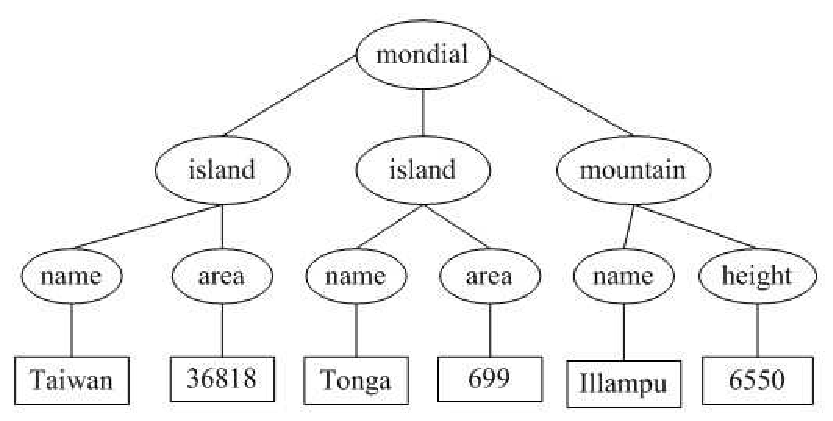
\includegraphics[width=0.4\textwidth]{XML}
\caption{树状结构}\label{fig:xml}
\vspace{\baselineskip}
\end{figure}


其插入图片的代码及其说明如下。
\vspace{1em}\noindent\hrule
\begin{verbatim}
\begin{figure}[htbp]
\centering
\includegraphics[width=0.4\textwidth]{文件名(.eps)}
\caption{标题}\label{标签名(通常为 fig:labelname)}
\vspace{\baselineskip} %表示图与正文空一行
\end{figure}
\end{verbatim}

\noindent\hrule

\begin{verbatim}
figure环境的可选参数[htbp]表示浮动图形所放置的位置,h (here)表示当前位置,t (top)表示页芯顶部,b (bottom)表示页芯底部,p (page)表示单独一页。在Word等软件中,图片通常插入到当前位置,如果当前页的剩余空间不够,图片将被移动到下一页,当前页就会出现很大的空白,其人工调整工作非常不便。由LaTeX提供的浮动图片功能,总是会按h->t->b->p的次序处理选项中的字母,自动调整图片的位置,大大减轻了工作量。
\centering命令将后续内容转换成每行皆居中的格式。
"\includegraphics"的可选参数用来设置图片插入文中的水平宽度,一般表示为正文宽度(\textwidth)的倍数。
\caption命令可选参数“标签名”为英文形式,一般不以图片或表格的数字顺序作为标签,而应包含一定的图片或表格信息,以便于文中引用(若图片、表格、公式、章节和参考文献等在文中出现的先后顺序发生了变化,其标注序号及其文中引用序号也会跟着发生变化,这一点是Word等软件所不能做到的)。另外,图题或表题并不会因为分页而与图片或表格体分置于两页,章节等各级标题也不会置于某页的最底部,LaTeX系统会自动调整它们在正文中的位置,这也是Word等软件所无法匹敌的。
\vspace将产生一定高度的竖直空白,必选参数为负值表示将后续文字位置向上提升,参数值可自行调整。em为长度单位,相当于大写字母M的宽度。\vspace{\baselineskip} 表示图与正文空一行。
引用方法:“见图~\ref{fig:figname}”、“如图~\ref{fig:figname}~所示”等。
\end{verbatim}

\noindent\hrule\vspace{1em}

若需要将~2~张及以上的图片并排插入到一行中,则需要采用\verb|minipage|环境,如图~\ref{fig:dd}~和图~\ref{fig:ds}~所示。
\begin{figure}[htbp]
\centering
\begin{minipage}{0.4\textwidth}
\centering
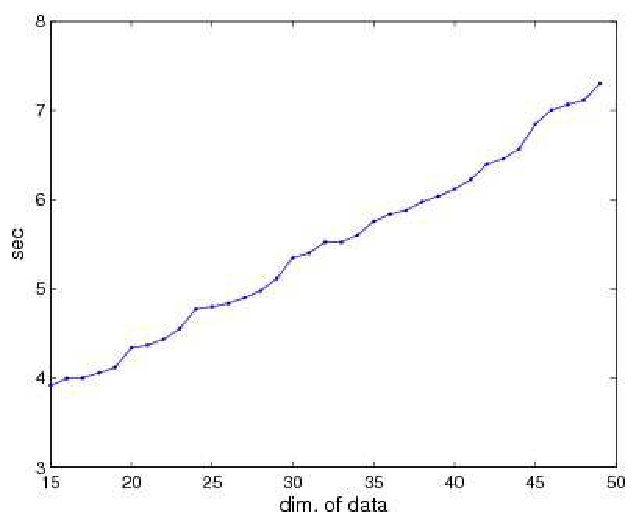
\includegraphics[width=\textwidth]{dataDimensions}
\caption{数据维数的变化}\label{fig:dd}
\end{minipage}
\begin{minipage}{0.4\textwidth}
\centering
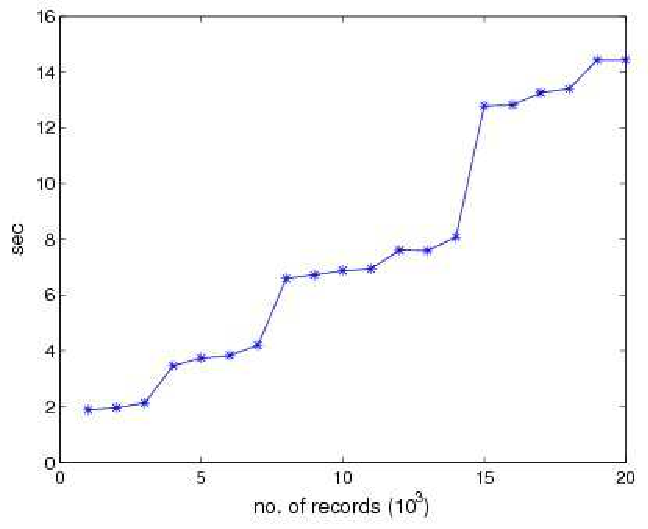
\includegraphics[width=\textwidth]{dataSize}
\caption{数据规模的变化}\label{fig:ds}
\end{minipage}
\vspace{\baselineskip}
\end{figure}

其代码如下所示。
\vspace{1em}\noindent\hrule
\begin{verbatim}
\begin{figure}[htbp]
\centering
\begin{minipage}{0.4\textwidth}
\centering
\includegraphics[width=\textwidth]{文件名}
\caption{标题}\label{fig:f1}
\end{minipage}
\begin{minipage}{0.4\textwidth}
\centering
\includegraphics[width=\textwidth]{文件名}
\caption{标题}\label{fig:f2}
\end{minipage}\vspace{\baselineskip}
\end{figure}
\end{verbatim}

\noindent\hrule

\begin{verbatim}
minipage环境的必选参数用来设置小页的宽度,若需要在一行中插入n个等宽图片,则每个小页的宽度应略小于(1/n)\textwidth。
\end{verbatim}

\noindent\hrule

\section{具有子图的图片插入方法}

图中若含有子图时,需要调用~subfigure~宏包, 如图~\ref{fig:subfig}~所示。
\begin{figure}[htbp]
  \centering
  \subfigure[Data Dimensions]{\label{fig:subfig:datadim}
                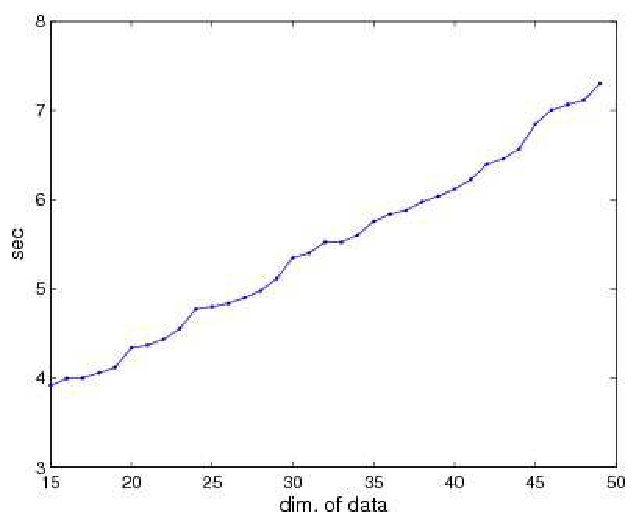
\includegraphics[width=0.4\textwidth]{dataDimensions}}
  \subfigure[Data Size]{\label{fig:subfig:datasize}
                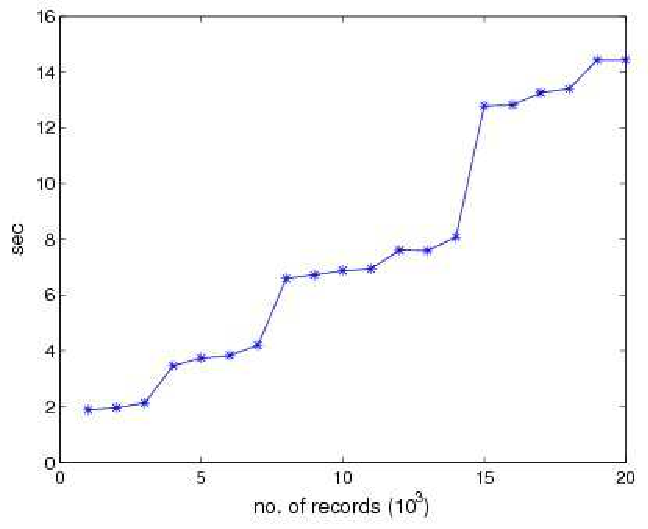
\includegraphics[width=0.4\textwidth]{dataSize}}
  \caption{Scalability of data}\label{fig:subfig}
\vspace{\baselineskip}
\end{figure}

其代码及其说明如下。
\vspace{1em}\noindent\hrule

\begin{verbatim}
\begin{figure}[htbp]
  \centering
  \subfigure[第1个子图标题]{
            \label{第1个子图标签(通常为 fig:subfig1:subsubfig1)}
            \includegraphics[width=0.4\textwidth]{文件名}}
  \subfigure[第2个子图标题]{
            \label{第2个子图标签(通常为 fig:subfig1:subsubfig2)}
            \includegraphics[width=0.4\textwidth]{文件名}}
  \caption{总标题}\label{总标签(通常为 fig:subfig1)}
\vspace{\baselineskip}
\end{figure}
\end{verbatim}

\noindent\hrule

\begin{verbatim}
子图的标签实际上可以随意设定,只要不重复就行。但为了更好的可读性,我们建议fig:subfig:subsubfig格式命名,这样我们从标签名就可以知道这是一个子图引用。
引用方法:总图的引用方法同本章第1节,子图的引用方法用\ref{fig:subfig:subsubfig}来代替。
\end{verbatim}

\noindent\hrule\vspace{1em}

子图的引用示例:如图~\ref{fig:subfig:datadim}~和图~\ref{fig:subfig:datasize}~所示。

若想获得插图方法的更多信息,参见网络上的~\href{ftp://ftp.tex.ac.uk/tex-archive/info/epslatex.pdf}{Using Imported Graphics in \LaTeX and pdf\LaTeX}~文档。 

\section{插入算法}

\begin{algorithm}[!h]
{
{
\renewcommand\baselinestretch{1.5}\selectfont %控制行距
\caption{ Scheduling Algorithm }
\label{alg:schedule}
\begin{algorithmic}[1]
\REQUIRE ~\\
A DFG $G=<V,E>$;\\
An allocation $A(G)$ for $G$.
\ENSURE ~\\
A schedule.
    \STATE{.......................}
    \FOR{$i\leftarrow\ 1\ to\ M$}    
        \STATE{.......................}
    \ENDFOR
    \STATE{.......................}
    \STATE{.......................}
    \STATE{.......................}
    \STATE{.......................}
    \STATE{.......................}
    \FOR{$k\leftarrow\ 1\ to\ |V|$}
        \STATE{.......................}
        \STATE{.......................}
        \STATE{.......................}
        \STATE{.......................}
    \IF{$LT_k==j$}
        \IF{there is no idle core in cluster $cl_{loc}$}
            \STATE{.......................}
            \STATE{.......................}
            \STATE{.......................}
            \STATE{.......................}
            \STATE{.......................}
            \STATE{.......................}
        \ELSE
            \STATE{.......................}
            \STATE{.......................}
            \STATE{.......................}
            \STATE{.......................}
            \STATE{.......................}
            \STATE{.......................}
        \ENDIF
    \ENDIF
    \ENDFOR
 

\end{algorithmic}
}
\par}
\end{algorithm}
%%% !Mode:: "TeX:UTF-8"

\chapter{表格的绘制方法}
\section{研究生毕业设计论文的绘表规范}

表应有自明性。表格不加左、右边线。表的编排建议采用国际通行的三线表。表内中文书写使用宋体五号字。

每个表格之上均应有表题(由表序和表名组成)。表序一般按章编排,如第~1~章第一个插表的序号为“表~1-1”等。表序与表名之间空两格,
表名使用中文五号字,居中。表名中不允许使用标点符号,表名后不加标点。
表头设计应简单明了,尽量不用斜线。表头中可采用化学,物理量等专业符号。

全表如用同一单位,则将单位符号移至表头右上角,加圆括号\cite{djy}。
表中数据应准确无误,书写清楚。数字空缺的格内加横线“-”(占~2~个数字宽度)。表内文字或数字上、下或左、右相同时,
采用通栏处理方式,不允许用“〃”、“同上”之类的写法。

表内文字使用宋体五号字,垂直居中书写,起行空一格、转行顶格、句末不加标点。
如某个表需要转页接排,在随后的各页上应重复表的编号。编号后加“(续表)”,表题可省略。续表应重复表头。
表格绘制完成之后,与正文空一行。

\section{普通表格的绘制方法}

表格应具有三线表格式,因此需要调用~booktabs~宏包,其标准格式如表~\ref{tab:table1}~所示。

\renewcommand\arraystretch{1.5}%控制行距
\begin{table}[!h]
\caption{基准测试集参数}\label{tab:bench}
\vspace{0.5em}
\centering
\begin{tabular}{l*{1}{C{2cm}}*{1}{L{6.2cm}}}
\toprule
Name         & $n$ & Description\\
\midrule
Random1      & 50  & Random graph generated by TGFF\\
Random2      & 100 & Random graph generated by TGFF\\
Random3      & 150 & Random graph generated by TGFF\\
Random4      & 200 & Random graph generated by TGFF\\
Random5      & 250 & Random graph generated by TGFF\\
Random6      & 300 & Random graph generated by TGFF\\
Random7      & 350 & Random graph generated by TGFF\\
Random8      & 400 & Random graph generated by TGFF\\
Random9      & 450 & Random graph generated by TGFF\\
Random10     & 500 & Random graph generated by TGFF\\
\bottomrule
\end{tabular}
\vspace{\baselineskip}
\end{table}
\renewcommand\arraystretch{1}

其绘制表格的代码及其说明如下。
\vspace{1em}\noindent\hrule

\begin{verbatim}
\begin{table}[htbp]
\caption{表标题}\label{标签名(通常为 tab:tablename)}
\vspace{0.5em}\centering\wuhao
\begin{tabular}{cc...c}
\toprule[1.5pt]
表头第1个格   & 表头第2个格   & ... & 表头第n个格  \\
\midrule[1pt]
表中数据(1,1) & 表中数据(1,2) & ... & 表中数据(1,n)\\
表中数据(2,1) & 表中数据(2,2) & ... & 表中数据(2,n)\\
表中数据(3,1) & 表中数据(3,2) & ... & 表中数据(3,n)\\
表中数据(4,1) & 表中数据(4,2) & ... & 表中数据(4,n)\\
...................................................\\
表中数据(m,1) & 表中数据(m,2) & ... & 表中数据(m,n)\\
\bottomrule[1.5pt]
\end{tabular}
\vspace{\baselineskip}
\end{table}
\end{verbatim}

\noindent\hrule

\begin{verbatim}
table环境是一个将表格嵌入文本的浮动环境。
\wuhao命令将表格的字号设置为五号字(10.5pt),在绘制表格结束退出时,不需要将字号再改回为\xiaosi,正文字号默认为小四号字(12pt)。
tabular环境的必选参数由每列对应一个格式字符所组成:c表示居中,l表示左对齐,r表示右对齐,其总个数应与表的列数相同。此外,@{文本}可以出现在任意两个上述的列格式之间,其中的文本将被插入每一行的同一位置。表格的各行以\\分隔,同一行的各列则以&分隔。
\toprule、\midrule和\bottomrule三个命令是由booktabs宏包提供的,其中\toprule和\bottomrule分别用来绘制表格的第一条(表格最顶部)和第三条(表格最底部)水平线,\midrule用来绘制第二条(表头之下)水平线,且第一条和第三条水平线的线宽为1.5pt,第二条水平线的线宽为1pt。
引用方法:“如表~\ref{tab:tablename}~所示”。
\end{verbatim}

\noindent\hrule

\section{长表格的绘制方法}

长表格是当表格在当前页排不下而需要转页接排的情况下所采用的一种表格环境。若长表格仍按照普通表格的绘制方法来获得,
其所使用的\verb|table|浮动环境无法实现表格的换页接排功能,表格下方过长部分会排在表格第1页的页脚以下。为了能够实现长表格的转页接排功能,
需要调用~longtable~宏包,由于长表格是跨页的文本内容,因此只需要单独的\verb|longtable|环境,所绘制的长表格的格式如表~\ref{tab:table2}~所示。

此长表格~\ref{tab:table2}~第~2~页的标题“编号(续表)”和表头是通过代码自动添加上去的,无需人工添加,若表格在页面中的竖直位置发生了变化,长表格在第~2~页
及之后各页的标题和表头位置能够始终处于各页的最顶部,也无需人工调整,\LaTeX~系统的这一优点是~Word~等软件所无法企及的。

下段内容是为了让下面的长表格分居两页,看到表标题“编号(续表)”的效果。摘录于《你若安好,便是晴天 -- 林徽因传》片段:

她叫林徽因,出生于杭州,是许多人梦中期待的白莲。她在雨雾之都伦敦,发生过一场空前绝后的康桥之恋。她爱过三个男子,爱得清醒,也爱得平静。徐志摩为她徜徉在康桥,深情地等待一场旧梦可以归来。梁思成与她携手走过千山万水,为完成使命而相约白头。金岳霖为她终身不娶,痴心不改地守候一世。可她懂得人生飘忽不定,要学会随遇而安。
真正的平静,不是避开车马喧嚣,而是在心中修篱种菊。尽管如流往事,每一天都涛声依旧,只要我们消除执念,便可寂静安然。愿每个人在纷呈世相中不会迷失荒径,可以端坐磐石上,醉倒落花前。
如果可以,请让我预支一段如莲的时光,哪怕将来某一天加倍偿还。这个雨季会在何时停歇,无从知晓。但我知道,你若安好,便是晴天。					
\wuhao\begin{longtable}{ccc}
\caption{湖南大学各学院名称一览}\label{tab:table2}
 \vspace{0.5em}\\
\toprule[1.5pt] 学院名称 & 网址 & 联系电话  \\ \midrule[1pt]
\endfirsthead
\multicolumn{3}{c}{表~\thetable(续表)}\vspace{0.5em}\\
\toprule[1.5pt] 学院名称 & 网址 & 联系电话  \\ \midrule[1pt]
\endhead
\bottomrule[1.5pt]
\endfoot
机械工程学院& \url{http://tdjxxy.tju.edu.cn/}& 87401979\\
精密仪器与光电子工程学院&  \url{http://www2.tju.edu.cn/colleges/precision/cn/}& 27404775\\
电子信息工程学院& \url{http://www.tju.edu.cn/seie}& 27406956\\
电气与自动化工程学院& \url{http://www2.tju.edu.cn/colleges/automate/}& 27405477\\
建筑工程学院& \url{http://www2.tju.edu.cn/colleges/civil/}& 27404072\\
化工学院& \url{http://chemeng.tju.edu.cn/}& 27403389\\
材料科学与工程学院& \url{http://mse.tju.edu.cn}& 27406693 \\
建筑学院& \url{http://hgw022072.chinaw3.com/}& 27402724-2111\\
求是学部\\
管理与经济学部&	\url{ http://sm.tju.edu.cn}& 27403423\\
理学院& \url{ http://www.tju.edu.cn/science/}& 27404118\\
文法学院& \url{ http://www2.tju.edu.cn/colleges/sociology/new/}& 27403691\\
软件学院& \url{http://scs.tju.edu.cn}& 87401540\\
计算机科学与技术学院& \url{http://cs.tju.edu.cn/}& 27406538\\
马克思主义学院& \url{http://www2.tju.edu.cn/colleges/marxism/}& 27405348\\
环境科学与工程学院& \url{http://www.tju.edu.cn/see}& 87402072\\
药物科学与技术学院& \url{http://www2.tju.edu.cn/colleges/pharmtier/}& 87401830\\
教育学院& \url{http://soe.tju.edu.cn/}& 27401028\\
职业技术教育学院& \url{http://202.113.0.248:8888}\\
继续教育学院& \url{http://aectu.tju.edu.cn/}& 27406298\\
仁爱学院& \url{http://www.tjrac.edu.cn/}& 68579990\\
农业与生物工程学院& \url{http://202.113.13.169/site/nongxueyuan/}& 87402171\\
国际教育学院 & \url{http://www.ietju.com/}& 27406147\\
网络教育学院 & \url{http://www.etju.com/}& 27426952 \\

\end{longtable}\xiaosi
\vspace{\baselineskip}

绘制长表格的代码及其说明如下。
\vspace{1em}\noindent\hrule

\begin{verbatim}
\wuhao\begin{longtable}{cc...c}
\caption{表标题}\label{标签名(通常为 tab:tablename)}\\
\toprule[1.5pt] 表头第1个格 & 表头第2个格 & ... & 表头第n个格\\ \midrule[1pt]
\endfirsthead
\multicolumn{n}{c}{表~\thetable(续表)}\vspace{0.5em}\\
\toprule[1.5pt] 表头第1个格 & 表头第2个格 & ... & 表头第n个格\\ \midrule[1pt]
\endhead
\bottomrule[1.5pt]
\endfoot
表中数据(1,1) & 表中数据(1,2) & ... & 表中数据(1,n)\\
表中数据(2,1) & 表中数据(2,2) & ... & 表中数据(2,n)\\
...................................................\\
表中数据(m,1) & 表中数据(m,2) & ... & 表中数据(m,n)\\
\end{longtable}\xiaosi
\end{verbatim}

\noindent\hrule
\begin{verbatim}
在绘制长表格的前面留出一个空白行,并在第2行的一开始全局定义长表格的字号为五号字,这样能够保证长表格之前段落的行距保持不变。
在绘制长表格结束后,需要\xiaosi命令重新将字号改为小四号字。
\endhead之前的文字描述的是第2页及其之后各页的标题或表头;
\endfirsthead之前的文字描述的是第1页的标题和表头,若无此命令,则第1页的表头和标题由\endhead命令确定;
同理,\endfoot之前的文字描述的是除最后一页之外每页的表格底部内容;
\endlastfoot之前的文字描述的是最后一页的表格底部内容,若无此命令,
则最后一页的表格底部内容由\endfoot命令确定;由于规范中长表格每页底部内容均相同(水平粗线),因此模板中没有用到\endlastfoot命令。
\end{verbatim}

\noindent\hrule
\section{列宽可调表格的绘制方法}
论文中能用到列宽可调表格的情况共有两种:一种是当插入的表格某一单元格内容过长以至于一行放不下的情况,
另一种是当对公式中首次出现的物理量符号进行注释的情况。这两种情况都需要调用~tabularx~宏包。下面将分别对这两种情况下可调表格的绘制方法进行阐述。
\subsection{表格内某单元格内容过长的情况}

首先给出这种情况下的一个例子如表~\ref{tab:table3}~所示。
\begin{table}[htbp]
\caption{最小的三个正整数的英文表示法}\label{tab:table3}
\vspace{0.5em}\wuhao
\begin{tabularx}{\textwidth}{llX}
\toprule[1.5pt]
Value & Name & Alternate names, and names for sets of the given size\\\midrule[1pt]
1 & One & ace, single, singleton, unary, unit, unity\\
2 & Two & binary, brace, couple, couplet, distich, deuce, double, doubleton, duad, duality, duet, duo, dyad, pair, snake eyes, span, twain, twosome, yoke\\
3 & Three & deuce-ace, leash, set, tercet, ternary, ternion, terzetto, threesome, tierce, trey, triad, trine, trinity, trio, triplet, troika, hat-trick\\\bottomrule[1.5pt]
\end{tabularx}
\vspace{\baselineskip}
\end{table}
绘制这种表格的代码及其说明如下。
\vspace{1em}\noindent\hrule
\begin{verbatim}
\begin{table}[htbp]
\caption{表标题}\label{标签名(通常为 tab:tablename)}
\vspace{0.5em}\wuhao
\begin{tabularx}{\textwidth}{l...X...l}
\toprule[1.5pt]
表头第1个格   & ... & 表头第X个格   & ... & 表头第n个格  \\
\midrule[1pt]
表中数据(1,1) & ... & 表中数据(1,X) & ... & 表中数据(1,n)\\
表中数据(2,1) & ... & 表中数据(2,X) & ... & 表中数据(2,n)\\
.........................................................\\
表中数据(m,1) & ... & 表中数据(m,X) & ... & 表中数据(m,n)\\
\bottomrule[1.5pt]
\end{tabularx}
\vspace{\baselineskip}
\end{table}
\end{verbatim}

\noindent\hrule
\begin{verbatim}
tabularx环境共有两个必选参数:第1个参数用来确定表格的总宽度,这里取为排版表格能达到的最大宽度——正文宽度\textwidth;第2个参数用来确定每列格式,其中标为X的项表示该列的宽度可调,其宽度值由表格总宽度确定。
标为X的列一般选为单元格内容过长而无法置于一行的列,这样使得该列内容能够根据表格总宽度自动分行。若列格式中存在不止一个X项,则这些标为X的列的列宽相同,因此,一般不将内容较短的列设为X。
标为X的列均为左对齐,因此其余列一般选为l(左对齐),这样可使得表格美观,但也可以选为c或r。
\end{verbatim}

\noindent\hrule
\subsection{对物理量符号进行注释的情况}
为使得对公式中物理量符号注释的转行与破折号“———”后第一个字对齐,此处最好采用表格环境。此表格无任何线条,左对齐,
且在破折号处对齐,一共有“式中”二字、物理量符号和注释三列,表格的总宽度可选为文本宽度,因此应该采用\verb|tabularx|环境。
由\verb|tabularx|环境生成的对公式中物理量符号进行注释的公式如式(\ref{eq:1})所示。
%\vspace*{10pt}

\begin{equation}\label{eq:1}
\ddot{\boldsymbol{\rho}}-\frac{\mu}{R_{t}^{3}}\left(3\mathbf{R_{t}}\frac{\mathbf{R_{t}\rho}}{R_{t}^{2}}-\boldsymbol{\rho}\right)=\mathbf{a}
\end{equation}

\begin{tabularx}{\textwidth}{@{}l@{\quad}r@{———}X@{}}
式中& $\bm{\rho}$ &追踪飞行器与目标飞行器之间的相对位置矢量;\\
&  $\bm{\ddot{\rho}}$&追踪飞行器与目标飞行器之间的相对加速度;\\
&  $\mathbf{a}$   &推力所产生的加速度;\\
&  $\mathbf{R_t}$ & 目标飞行器在惯性坐标系中的位置矢量;\\
&  $\omega_{t}$ & 目标飞行器的轨道角速度;\\
&  $\mathbf{g}$ & 重力加速度,$=\frac{\mu}{R_{t}^{3}}\left(
3\mathbf{R_{t}}\frac{\mathbf{R_{t}\rho}}{R_{t}^{2}}-\bm{\rho}\right)=\omega_{t}^{2}\frac{R_{t}}{p}\left(
3\mathbf{R_{t}}\frac{\mathbf{R_{t}\rho}}{R_{t}^{2}}-\bm{\rho}\right)$,这里~$p$~是目标飞行器的轨道半通径。
\end{tabularx}
\vspace{\wordsep}

其中生成注释部分的代码及其说明如下。

\vspace{1em}\noindent\hrule

\begin{verbatim}
\begin{tabularx}{\textwidth}{@{}l@{\quad}r@{— — —}X@{}}
式中 & symbol-1 & symbol-1的注释内容;\\
     & symbol-2 & symbol-2的注释内容;\\
     .............................;\\
     & symbol-m & symbol-m的注释内容。
\end{tabularx}\vspace{\wordsep}
\end{verbatim}

\noindent\hrule

\begin{verbatim}
tabularx环境的第1个参数选为正文宽度,第2个参数里面各个符号的意义为:
    第1个@{}表示在“式中”二字左侧不插入任何文本,“式中”二字能够在正文中左对齐,若无此项,则“式中”二字左侧会留出一定的空白;
    @{\quad}表示在“式中”和物理量符号间插入一个空铅宽度的空白;
    @{— — —}实现插入破折号的功能,它由三个1/2的中文破折号构成;
    第2个@{}表示在注释内容靠近正文右边界的地方能够实现右对齐。
\end{verbatim}

\noindent\hrule\vspace{1em}

由此方法生成的注释内容应紧邻待注释公式并置于其下方,因此不能将代码放入\verb|table|浮动环境中。但此方法不能实现自动转页接排,
可能会在当前页剩余空间不够时,全部移动到下一页而导致当前页出现很大空白。因此在需要转页处理时,还请您手动将需要转页的代码放入一个
新的\verb|tabularx|环境中,将原来的一个\verb|tabularx|环境拆分为两个\verb|tabularx|环境。

若想获得绘制表格的更多信息,参见网络上的~\href{http://www.tug.org/pracjourn/2007-1/mori/}{Tables in \LaTeXe: Packages and Methods}~文档。


%%% !Mode:: "TeX:UTF-8"

\chapter{数学公式的输入方法}
\section{研究生毕业设计论文的公式规范}

论文中的公式应另起行,原则上应居中书写,与周围文字留有足够的空间区分开。
若公式前有文字(如“解”、“假定”等),文字空两格写,公式仍居中写。公式末不加标点。

公式应标注序号,并将序号置于括号内。 公式序号按章编排,如第~1~章第一个公式序号为“(1-1)”。公式的序号右端对齐。

公式较长时最好在等号“=”处转行,如难实现,则可在~$+$、$-$、$\times$、$\div$~运算符号处转行,转行时运算符号仅书写于转行式前,不重复书写。

文中引用公式时,一般用“见式~(1-1)”或“由公式~(1-1)”。

公式中用斜线表示“除”的关系时应采用括号,以免含糊不清,如~$a/(b\cos x)$。通常“乘”的关系在前,如~$a\cos x/b$而不写成~$(a/b)\cos x$。

不能用文字形式表示等式,如:$\textnormal{刚度}=\frac{{\textnormal{受力}}}{{\textnormal{受力方向的位移}}}$。

对于数学公式的输入方法,网络上有一个比较全面权威的文档\textbf{~\href{http://tug.ctan.org/cgi-bin/ctanPackageInformation.py?id=voss-mathmode}{Math mode}}~请大家事先大概浏览一下。下面将对学位论文中主要用到的数学公式排版形式进行阐述。

\section{生成~\LaTeX~数学公式的两种方法}
对于先前没有接触过~\LaTeX~的人来说,编写~\LaTeX~数学公式是一件很繁琐的事,尤其是对复杂的数学公式来说,更可以说是一件难以完成的任务。
实际上,生成~\LaTeX~数学公式有两种较为简便的方法,一种是基于~MathType~数学公式编辑器的方法,另一种是基于~MATLAB~商业数学软件的方法,
下面将分别对这两种数学公式的生成方法作一下简单介绍。

\subsection{基于~MathType~软件的数学公式生成方法}
MathType~是一款功能强大的数学公式编辑器软件,能够用来在文本环境中插入~Windows OLE~图形格式的复杂数学公式,所以应用比较普遍。但此软件只有~30~天的试用期,之后若再继续使用则需要付费购买才行。网络上有很多破解版的~MathType~软件可供下载免费使用,
笔者推荐下载安装版本号在~6.5~之上的中文破解版。

在安装好~MathType~之后,若在输入窗口中编写数学公式,复制到剪贴板上的仍然是图形格式的对象。
若希望得到可插入到~\LaTeX~编辑器中的文本格式对象,则需要对~MathType~软件做一下简单的设置:在~MathType~最上排的按钮中依次选择“参数选项
$\to$转换”,在弹出的对话窗中选中“转换到其它语言(文字):”,在转换下拉框中选择“Tex~--~--~LaTeX 2.09 and later”,并将对话框最下方的两个复选框全部勾掉,点击确定,这样,再从输入窗口中复制出来的对象就是文本格式的了,就可以直接将其粘贴到~\LaTeX~
编辑器中了。按照这种方法生成的数学公式两端分别有标记\verb|\[|和标记\verb|\]|,在这两个标记之间才是真正的数学公式代码。

若希望从~MathType~输入窗口中复制出来的对象为图形格式,则只需再选中“公示对象(Windows OLE~图形)”即可。

\subsection{基于~MATLAB~软件的数学公式生成方法}

MATLAB~是矩阵实验室(Matrix Laboratory)的简称,是美国~MathWorks~公司出品的商业数学软件。它是当今科研领域最常用的应用软件之一,
具有强大的矩阵计算、符号运算和数据可视化功能,是一种简单易用、可扩展的系统开发环境和平台。

MATLAB~中提供了一个~latex~函数,它可将符号表达式转化为~\LaTeX~数学公式的形式。其语法形式为~latex(s),其中,~s~为符号表达式,
之后再将~latex~函数的运算结果直接粘贴到~\LaTeX~编辑器中。从~\LaTeX~数学公式中可以发现,其中可能包含如下符号组合:

\begin{verbatim*}
\qquad=两个空铅(quad)宽度
\quad=一个空铅宽度
\;=5/18空铅宽度
\:=4/18空铅宽度
\,=3/18空铅宽度
\!=-3/18空铅宽度
\ =一个空格
\end{verbatim*}

所以最好将上述符号组合从数学公式中删除,从而使数学公式显得匀称美观。

对于~Word~等软件的使用者来说,在我们通过~MATLAB~运算得到符号表达式形式的运算结果时,在~Word~中插入运算结果需要借助于~MathType~软件,
通过在~MathType~中输入和~MATLAB~运算结果相对应的数学表达形式,之后再将~MathType~数学表达式转换为图形格式粘贴到~Word~中。实际上,
也可以将~MATLAB~中采用~latex~函数运行的结果直接粘贴到~MathType~中,再继续上述步骤,这样可以大大节省输入公式所需要的时间。
此方法在~MathType~6.5c~上验证通过,若您粘入到~MathType~中的仍然为从~MATLAB~中导入的代码,请您更新~MathType~软件。

\section{数学字体}
在数学模式下,常用的数学字体命令有如下几种:

\begin{verbatim}
\mathnormal或无命令 用数学字体打印文本;
\mathit             用斜体(\itshape)打印文本;
\mathbf             用粗体(\bfseries)打印文本;
\mathrm             用罗马体(\rmfamily)打印文本;
\mathsf             用无衬线字体(\sffamily)打印文本;
\mathtt             用打印机字体(\ttfamily)打印文本;
\mathcal            用书写体打印文本;
\end{verbatim}

在学位论文撰写中,只需要用到上面提到的~\verb|\mathit|、\verb|\mathbf|~和~\verb|\mathrm|~命令。若要得到~Times New Roman~的数学字体,则需要调用~txfonts~宏包(此宏包实际上采用的是~Nimbus Roman No9 L~字体,
它是开源系统中使用的免费字体,其字符字体与~Times New Roman~字体几乎完全相同);若要得到粗体数学字体,则需要调用~bm~宏包。表~\ref{tab:fonts}~中分别列出了得到阿拉伯数字、拉丁字母和希腊字母
各种数学字体的命令。

\begin{table}[htbp]
\caption{常用数学字体命令一览}\label{tab:fonts}
\vspace{0.5em}\centering\wuhao
\begin{tabular}{llll}
\toprule
 & 阿拉伯数字\&大写希腊字母 & 大小写拉丁字母 & 小写希腊字母  \\
\midrule
斜体 & \verb|\mathit{}| & \verb|无命令| & \verb|无命令|\\
粗斜体 & \verb|\bm{\mathit{}}| & \verb|\bm{}| & \verb|\bm{}|\\
直立体 & \verb|无命令| & \verb|\mathrm{}| & \verb|字母后加up|\\
粗体 & \verb|\mathbf{}或\bm{}| & \verb|\mathbf{}| & \verb|\bm{字母后加up}|\\
\bottomrule
\end{tabular}
\vspace{\baselineskip}
\end{table}

\noindent 下面列出了一些应采用直立数学字体的数学常数和数学符号。

\vspace{-0.5em}\begin{center}\begin{tabularx}{0.7\textwidth}{XX}
$\mathrm{d}$、 $\mathrm{D}$、 $\mathrm{p}$~———微分算子 & $\mathrm{e}$~———自然对数之底数\\
$\mathrm{i}$、 $\mathrm{j}$~———虚数单位 & $\piup$———圆周率\\
\end{tabularx}\end{center}

\section{行内公式}
出现在正文一行之内的公式称为行内公式,例如~$f(x)=\int_{a}^{b}\frac{\sin{x}}{x}\mathrm{d}x$。对于非矩阵和非多行形式的行内公式,一般不会使得行距发生变化,而~Word~等软件却会根据行内公式的竖直距离而自动调节行距,如图~\ref{fig:hangju}~所示。

\begin{figure}[htbp]
\centering
\subfigure[由~\LaTeX~系统生成的行内公式]{\label{fig:subfig:latex}
                \fbox{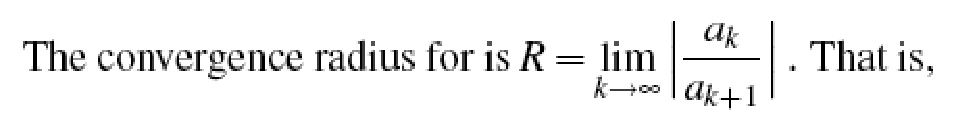
\includegraphics[width=0.55\textwidth]{latex}}}
\subfigure[由~Word软件生成的~.doc~格式行内公式]{\label{fig:subfig:word}
                \fbox{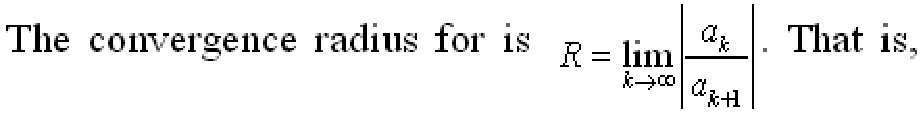
\includegraphics[width=0.55\textwidth]{word}}}
\subfigure[由~Word软件生成的~.pdf~格式行内公式]{\label{fig:subfig:pdf}
                \fbox{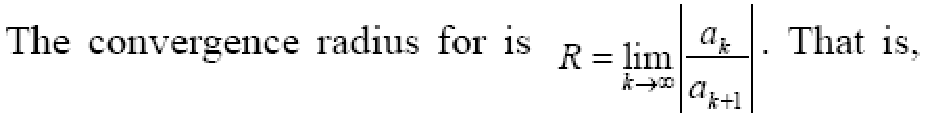
\includegraphics[width=0.55\textwidth]{pdf}}}

\caption{由~\LaTeX~和~Word~生成的~3~种行内公式屏显效果}\label{fig:hangju}
\vspace{-1em}
\end{figure}

这三幅图分别为~\LaTeX~和~Word~生成的行内公式屏显效果,从图中可看出,在~\LaTeX~文本含有公式的行内,在正文与公式之间对接工整,行距不变;而在~Word~文本含有公式的行内,在正文与公式之间对接不齐,行距变大。因此从这一点来说,
\LaTeX~系统在数学公式的排版上具有很大优势。

\LaTeX~提供的行内公式最简单、最有效的方法是采用~\TeX~本来的标记———开始和结束标记都写作~\$,例如本段开始的例子可由下面的输入得到。
\verb|$f(x)=\int_{a}^{b}\frac{\sin{x}}{x}\mathrm{d}x$|

\section{行间公式}
位于两行之间的公式称为行间公式,每个公式都是一个单独的段落,例如
\[\int_a^b{f\left(x\right)\mathrm{d}x}=\lim_{\left\|\Delta{x_i}\right\|\to 0}\sum_i{f\left(\xi_i\right)\Delta{x_i}}\]
除人工编号外,\LaTeX~各种类型行间公式的标记见表~\ref{tab:eqtag}。
\begin{table}[htbp]
\caption{各种类型行间公式的标记}\label{tab:eqtag}
\vspace{0.5em}\centering\wuhao
\begin{tabularx}{\textwidth}{cll}
\toprule
& 无编号 & 自动编号\\
\midrule
单行公式& \verb|\begin{displaymath}... \end{displaymath}|& \verb|\begin{equation}... \end{equation}|\\
        & 或~\verb|\[...\]| & \\
多行公式& \verb|\begin{eqnarray*}... \end{eqnarray*}|& \verb|\begin{eqnarray}... \end{eqnarray}|\\
\bottomrule
\end{tabularx}
\end{table}

另外,在自动编号的某行公式行尾添加标签~\verb|\nonumber|,可将该行转换为无编号形式。

行间多行公式需采用~\verb|eqnarray|~或~\verb|eqnarray*|~环境,它默认是一个列格式为~\verb|rcl|~的~3~列矩阵,并且中间列的字号要小一些,因此通常只将需要对齐的运算符号(通常为等号“=”)置于中间列。

\section{可自动调整大小的定界符}
若在左右两个定界符之前分别添加命令~\verb|\left|~和~\verb|\right|,则定界符可根据所包围公式大小自动调整其尺寸,这可从式(\ref{nodelimiter})和式(\ref{delimiter})中看出。
\begin{equation}\label{nodelimiter}
(\sum_{k=\frac12}^{N^2})
\end{equation}
\begin{equation}\label{delimiter}
\left(\sum_{k=\frac12}^{N^2}\right)
\end{equation}
式(\ref{nodelimiter})和式(\ref{delimiter})是在~\LaTeX~中分别输入如下代码得到的。
\begin{verbatim}
(\sum_{k=\frac12}^{N^2})
\left(\sum_{k=\frac12}^{N^2}\right)
\end{verbatim}
\verb|\left|~和~\verb|\right|~总是成对出现的,若只需在公式一侧有可自动调整大小的定界符,则只要用“.”代替另一侧那个无需打印出来的定界符即可。

若想获得关于此部分内容的更多信息,可参见~\href{http://tug.ctan.org/cgi-bin/ctanPackageInformation.py?id=voss-mathmode}{Math mode}~文档的第~8~章“Brackets, braces and parentheses”。

\section{数学重音符号}
数学重音符号通常用来区分同一字母表示的不同变量,输入方法如下(需要调用~\verb|amsmath|~宏包):

\vspace{0.5em}\noindent\wuhao\begin{tabularx}{\textwidth}{Xc|Xc|Xc}
 \verb|\acute| & $\acute{a}$ & \verb|\mathring| & $\mathring{a}$ & \verb|\underbrace| & $\underbrace{a}$ \\
 \verb|\bar| & $\bar{a}$ & \verb|\overbrace| & $\overbrace{a}$ & \verb|\underleftarrow| & $\underleftarrow{a}$ \\
 \verb|\breve| & $\breve{a}$ & \verb|\overleftarrow| & $\overleftarrow{a}$ & \verb|\underleftrightarrow| & $\underleftrightarrow{a}$ \\
 \verb|\check| & $\check{a}$ & \verb|\overleftrightarrow| & $\overleftrightarrow{a}$ & \verb|\underline| & $\underline{a}$ \\
 \verb|\dddot| & $\dddot{a}$ & \verb|\overline| & $\overline{a}$ & \verb|\underrightarrow| & $\underrightarrow{a}$ \\
 \verb|\ddot| & $\ddot{a}$ & \verb|\overrightarrow| & $\overrightarrow{a}$ & \verb|\vec| & $\vec{a}$ \\
 \verb|\dot| & $\dot{a}$ & \verb|\tilde| & $\tilde{a}$ & \verb|\widehat| & $\widehat{a}$ \\
 \verb|\grave| & $\grave{a}$ & \verb|\underbar| & $\underbar{a}$ & \verb|\widetilde| & $\widetilde{a}$ \\
 \verb|\hat| & $\hat{a}$
\end{tabularx}\vspace{0.5em}
\xiaosi 当需要在字母~$i$~和~$j$~的上方添加重音符号时,为了去掉这两个字母顶上的小点,这两个字母应该分别改用~\verb|\imath|~和~\verb|\jmath|。

如果遇到某些符号不知道该采用什么命令能输出它时,则可通过~\href{http://detexify.kirelabs.org/classify.html}{Detexify$^2$~网站}来获取符号命令。若用鼠标左键在此网页的方框区域内画出你所要找的符号形状,则会在网页右方列出和你所画符号形状相近的~5~个符号及其相对应的~\LaTeX~输入命令。若所列出的符号中不包括你所要找的符号,还可通过点击“Select from the complete list!”的链接以得分从低到高的顺序列出所有符号及其相对应的~\LaTeX~输入命令。

最后,建议大家还以~\href{http://tug.ctan.org/cgi-bin/ctanPackageInformation.py?id=voss-mathmode}{Math mode}~这篇~pdf~文档作为主要参考。若要获得最为标准、美观的数学公式排版形式,可以查查文档中是否有和你所要的排版形式相同或相近的代码段,通过修改代码段以获得你所要的数学公式排版形式。


%%% !Mode:: "TeX:UTF-8"

\chapter{罗列和定理环境使用方法}

\section{单层罗列环境}
湖南大学学位论文一般可采用两种罗列环境:一种是并列条目有同样标签的~\verb|itemize|~罗列环境,另一种是具有自动排序编号符号的~\verb|enumerate|~罗列环境。这两种罗列环境的样式参数可参考图~\ref{fig:list}。
\begin{figure}[htbp]
\centering
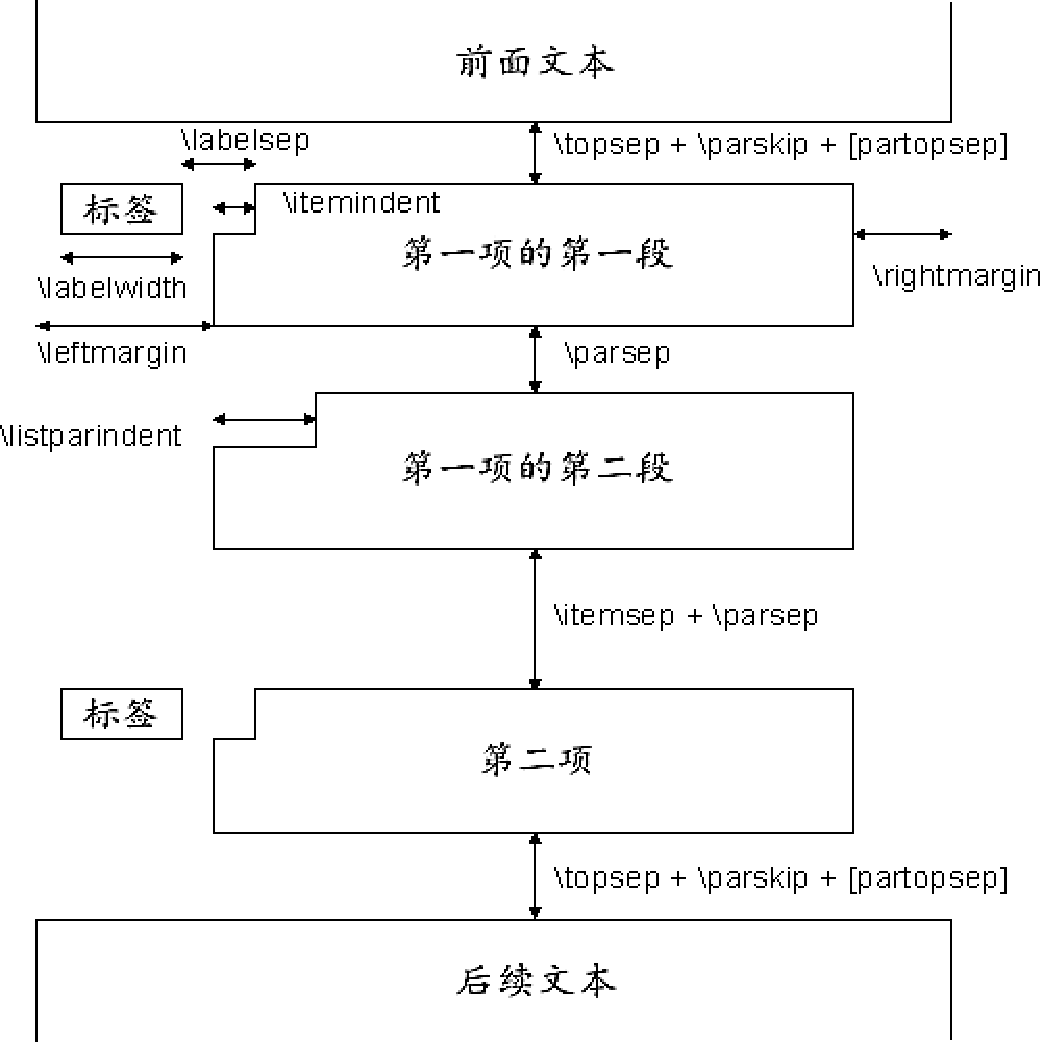
\includegraphics[width = 0.6\textwidth]{list}
\caption{罗列环境参数示意图}\label{fig:list}\vspace{-1em}
\end{figure}

通过调用~enumitem~宏包可以很方便地控制罗列环境的布局,其~format.tex~文件中的~\verb|\setitemize|~和~\verb|\setenumerate|~命令分别用来设置~\verb|itemize|~和~\verb|enumerate|~环境的样式参数。采用~\verb|itemize|~单层罗列环境的排版形式如下:

\begin{itemize}
\item 第一个条目文本内容
\item 第二个条目文本内容
\item 第三个条目文本内容
\end{itemize}

其代码如下

\begin{verbatim}
\begin{itemize}
  \item 第一个条目文本内容
  \item 第二个条目文本内容
  ...
  \item 第三个条目文本内容
\end{itemize}
\end{verbatim}

采用~\verb|enumerate|~单层罗列环境的排版形式如下:

\begin{enumerate}
\item 第一个条目文本内容
\item 第二个条目文本内容
\item 第三个条目文本内容
\end{enumerate}

其代码如下

\begin{verbatim}
\begin{enumerate}
  \item 第一个条目文本内容
  \item 第二个条目文本内容
  ...
  \item 第三个条目文本内容
\end{enumerate}
\end{verbatim}



\section{定理环境}

\begin{definition}[谱半径]\label{def:def1}
  称~$n$~阶方阵~$\mathbf{A}$~的全体特征值~$\lambda_1,\cdots,\lambda_n$~组成的集合为~$\mathbf{A}$~的谱,称
  $$\rho(\mathbf{A})=\max{\{|\lambda_1|,\cdots,|\lambda_n|\}}$$
\end{definition}
\begin{theorem}[相似充要条件]\label{lemma:l1}
  方阵$A$和$B$相似的充要条件是:~$A$~和~$B$~有全同的不变因子。
\end{theorem}
\begin{corollary}[推论1]\label{cor:cor1}
在赋范空间~$(X,\|\cdot\|)$~上定义~$d(x,y)=\|x-y\|$, 对任意~$x,y\in X$,~则~$(X,d)$~是距离空间。
\end{corollary}
\begin{proof}
  只需证明~$d(x,y)$~是距离。
\end{proof}
\newpage

定义代码如下:
\begin{verbatim}
 \begin{definition}[谱半径]\label{def:def1}
  称~$n$~阶方阵~$\mathbf{A}$~的全体特征值
  $\lambda_1,\cdots,\lambda_n$组成的集合为~$\mathbf{A}$~的谱,称
  $$\rho(\mathbf{A})=\max{\{|\lambda_1|,\cdots,|\lambda_n|\}}$$
\end{definition}
\end{verbatim}
\noindent\hrule

\vspace{0.1em}\noindent\hrule
\vspace{1em}
定理代码如下:
\begin{verbatim}
\begin{theorem}[相似充要条件]\label{lemma:l1}
  方阵$A$和$B$相似的充要条件是:$A$和$B$有全同的不变因子。
\end{theorem}
\end{verbatim}
\noindent\hrule\vspace{0.1em}

\noindent\hrule
\vspace{1em}
推论和证明代码如下:
\begin{verbatim}
\begin{corollary}[推论1]\label{cor:cor1}
在赋范空间~$(X,\|\cdot\|)$~上定义$d(x,y)=\|x-y\|$,
对任意$x,y\in X$,则$(X,d)$是距离空间。
\end{corollary}
\begin{proof}
  只需证明$d(x,y)$是距离。
\end{proof}
\end{verbatim}
\noindent\hrule\vspace{1em}

定理定义[]中是可选参数,用来说明定理的名称。其他环境格式书写与上面定理、定义、推论格式相同,可自己调用其他环境。
若需要书写定理定义等内容,而且带有顺序编号,需要采用如下环境。除了~\verb|proof|~环境之外,其余~9~个环境都可以有一个可选参数作为附加标题。

\begin{center}
\vspace{0.5em}\noindent\wuhao\begin{tabularx}{0.7\textwidth}{lX|lX}
定理 & \verb|theorem|~环境 & 定义 & \verb|definition|~环境 \\
例 & \verb|example|~环境 & 算法 & \verb|algorithm|~环境 \\
公理 & \verb|axiom|~环境 & 命题 & \verb|proposition|~环境 \\
引理 & \verb|lemma|~环境 & 推论 & \verb|corollary|~环境 \\
注解 & \verb|remark|~环境 & 证明 & \verb|proof|~环境 \\
\end{tabularx}
\end{center} 
%%\section{conclusion}
\label{sec:conclusion}
%\del{In this paper, we have proved the Min-Min  SRLG-Disjoint routing problem is NP-complete.}
In this paper, we propose an efficient algorithm to solve the Min-Min  SRLG-Disjoint routing problem in the presence of the trap problem. To reduce the complexity of searching for the alternative pair, we propose a divide-and-conquer solution to partition the original Min-Min SRLG-Disjoint routing problem into multiple sub-problems based on a SRLG conflicting link set derived from the AP path encountering the trap problem. Our algorithm takes advantage of existing AP search results and parallel executions for significantly faster path finding.
We have conducted extensive simulations  using the topology trace  on a multi-core CPU platform. The simulation results demonstrate that our algorithm can outperform other approaches with higher routing performance while at a much higher search speed.

\end{verbatim}
那么,编译的时候就只编译未加~\%~的一章,在这个例子中,即本章~intros。

理论上,并不一定要把每章放在不同的文件中。但是这种自顶向下,分章节写作、编译的方法有利于提高效率,大大减少~Debug~过程中的编译时间,同时减小风险。

\section{参考文献生成方法}

\LaTeX~具有插入参考文献的能力。Google Scholar~网站上存在兼容~BibTeX~的参考文献信息,通过以下几个步骤,可以轻松完成参考文献的生成。
\begin{itemize}
  \item 在\href{http://scholar.google.com/}{谷歌学术搜索}中,
        点击\href{http://scholar.google.com/scholar_preferences?hl=en&as_sdt=0,5}{学术搜索设置}。
  \item 页面打开之后,在\textbf{文献管理软件}选项中选择\textbf{显示导入~BibTeX~的链接},单击保存设置,退出。
  \item 在谷歌学术搜索中检索到文献后,在文献条目区域单击导入~BibTeX~选项,页面中出现文献的引用信息。
  \item 将文献引用信息的内容复制之后,添加到~references~文件夹下的~reference.bib~中。
\end{itemize}

\section{编译注意事项}
\begin{enumerate}
  \item 由于模板使用~UTF-8~编码,所以源文件应该保存成~UTF-8~格式,否则可能出现中文字符无法识别的错误。
  本模板中每一个~.tex~文件的文件的开头已经加上一行:\\
    \verb|% !Mode:: "TeX:UTF-8"|\\
     这样可以确保~.tex~文件默认使用~UTF-8~的格式打开。读者如果删去此行,很有可能会导致中文字符显示乱码。
     在~WinEdt~编辑器中可以使用以下两种方式保存成~UTF-8~格式:
      \begin{enumerate}
        \item 先建立~.tex~文件,另存为~.tex~文件时,选择用~UTF-8~格式保存。
        \item
            在~WinEdt~编辑器中,选择\\
            \mbox{~Document$\to$Document Settings$\to$Document Mode $\to$TeX:UTF-8} 同时在~WinEdt~最下面的状态栏中,可以看到该文档是~TeX~格式还是~TeX:UTF-8~格式。
            当文档为~TeX:UTF-8~格式时,状态栏一般显示:
            \makebox[\textwidth][l]{Wrap | Indent | INS | LINE |Spell | TeX:UTF-8 | -src~等。}
      \end{enumerate}
  \item 如果在pdf书签中,中文显示乱码的话,则注意以下说明:
    \begin{verbatim}
        \usepackage{CJKutf8}
        % 1. 如果使用CJKutf8
        %    Hyperref中应使用unicode参数
        % 2. 如果使用CJK
        %    Hyperref则使用CJKbookmarks参数
        %    可惜得到的PDF书签是乱码,建议弃用
        % 3. Unicode选项和CJKbookmarks不能同时使用
        \usepackage[
        %CJKbookmarks=true,
        unicode=true
        ]{hyperref}
     \end{verbatim}
 \item 建议采用以下两种编译方式:
  \begin{enumerate}
     \item latex + bibtex + latex + latex + dvi2pdf. 在这种编译情况下,对应的~hnumain.tex~文件的第一行是\verb|\def\usewhat{dvipdfmx}|~(缺省设置)。 此时,所有图片文件应该保存为~.eps~格式,如~figures~文件夹里~.eps~图片。
          如果您选择在命令行中操作,可以在编译的时候依次输入~latex hnumain, bibtex hnumain, latex hnumain, latex hnumain~和~dvipdfmx hnumain, 编译完成之后,需要手动打开~pdf~文件。
     \item pdflatex + pdflatex. 在这种编译情况下,对应的~hnumain.tex~文件的第一行应该改为\verb|\def\usewhat{pdflatex}|~。 此时, 编译不支持~.eps~图片格式,此时需要在命令行下使用~epstopdf~指令将~figures~文件夹下 的~.eps~文件转化成~.pdf~文件格式,命令行中操作格式为~epstopdf a.eps~。
          在命令行编译的时候,依次输入~pdflatex hnumain~和~pdflatex hnumain, 编译完成之后,需要手动打开~pdf~文件。
  \end{enumerate}
\end{enumerate}

\section{系统要求}
    CTEX 2.8, MiKTeX 2.8, TeX Live 2009~或以上版本。使用推荐的~WinEdt 6.0~编辑器,可以完成文件的编辑和编译工作。

\section{\TeX~简介}

以下内容是~milksea@bbs.ctex.org~撰写的关于~\TeX~的简单介绍,略有改动。
注意这不是一个入门教程,不讲~\TeX~系统的配置安装,也不讲具体的~\LaTeX~代码。
这里仅仅试图以一些只言片语来解释:
进入这个门槛之前新手应该知道的注意事项,以及遇到问题以后该去如何解决问题。

\subsection{什么是 \TeX/\LaTeX,我是否应该选择它~?}

\TeX~是最早由高德纳(Donald Knuth)教授创建的一门标记式宏语言,
用来排版科技文章,尤其擅长处理复杂的数学公式。\TeX~同时也是处理这一语言的排版软件。
\LaTeX~是 Leslie Lamport 在~\TeX~基础上按内容/格式分离和模块化等思想建立的一集~\TeX~上的格式。

\TeX~本身的领域是专业排版领域
但现在~TeX/LaTeX~也被广泛用于生成电子文档甚至幻灯片等,~\TeX~语言的数学部分
偶尔也在其他一些地方使用。但注意~\TeX~并不适用于文书处理(Microsoft Office 的领域,以前和现在都不是)。

选择使用~\TeX/\LaTeX~的理由包括:
\begin{itemize}
\item 免费软件;
\item 专业的排版效果;
\item 是事实上的专业数学排版标准;
\item 广泛的西文期刊接收甚或只接收 LaTeX 格式的投稿;
\item[] ……
\end{itemize}
不选择使用~\TeX/\LaTeX~的理由包括:
\begin{itemize}
\item 需要相当精力学习;
\item 图文混合排版能力不够强;
\item 仅在数学、物理、计算机等领域流行;
\item 中文期刊的支持较差;
\item[] ……
\end{itemize}

请尽量清醒看待网上经常见到的关于~\TeX~与其他软件的优劣比较和口水战。在选择使用或离开之前,请先考虑
\TeX~的应用领域,想想它是否适合你的需要。


\subsection{我该用什么编辑器~?}

编辑器功能有简有繁,特色不一,从简单的纯文本编辑器到繁复的 Emacs,因人而易。基本功能有语法高亮、方便编译预览就很好了,扩充功能和定制有无限的可能。初学者可以使用功能简单、使用方便的专用编辑器,如 ~TeXWorks、Kile、WinEdt~等,或者类似所见即所得功能的~LyX;熟悉的人可以使用定制性更强的~Notepad++、SciTE、Vim、Emacs ~等。这方面的介绍很多,一开始不妨多试几种,找到最适合自己的才是最好的。

另外提醒一句,编辑器只是工作的助手,不必把它看得太重。

\subsection{我应该看什么~\LaTeX~读物~?}

这不是一个容易回答的问题,因为有许多选择,也同样有许多不合适的选择。
这里只是选出一个比较好的答案。更多更详细的介绍可以在版面和网上寻找(注意时效)。

近两年~\TeX~的中文处理发展很快,目前没有哪本书在中文处理方面给出一个最新进展的合适综述,
因而下面的介绍也不主要考虑中文处理。

\begin{enumerate}

\item 我能阅读英文。
\begin{enumerate}
\item 迅速入门:ltxprimer.pdf (LaTeX Tutorials: A Primer, India TUG)
\item 系统学习:A Guide to LaTeX, 4th Edition, Addison-Wesley
               有机械工业出版社的影印版(《\LaTeX{}~实用教程》)
\item 深入学习:要读许多书和文档,TeXbook 是必读的
\item 细节学习:去读你使用的每一个宏包的说明文档
\item 专题学习:阅读讲数学公式、图形、表格、字体等的专题文档
\end{enumerate}

\item 我更愿意阅读中文。
\begin{enumerate}
\item 迅速入门:lnotes.pdf (LaTeX Notes, 1.20, Alpha Huang)
\item 系统学习:《\LaTeXe{}~科技排版指南》,邓建松(电子版)
      如果不好找,可以阅读《\LaTeXe~入门与提高》第二版,陈志杰等,或者 《\LaTeXe~完全学习手册》,胡伟
\item 深入学习:~TeXbook0.pdf~(特可爱原本,TeXbook 的中译,xianxian)
\item 具体问题释疑:~CTeX-FAQ.pdf~,\\
        吴凌云,~\url{http://www.ctex.org/CTeXFAQ}~
\end{enumerate}
\end{enumerate}

遇见问题和解决问题的过程可以快速提高自己的技能,建议此时:
\begin{itemize}
  \item 利用~Google~搜索。
  \item 清楚,扼要地提出你的问题。
\end{itemize}

\subsection{什么知识会过时~?什么不会~?}

\TeX~是排版语言,也是广泛使用的软件,并且不断在发展中;
因此,总有一些东西会很快过时。作为学习~\TeX~的人,
免不了要看各种各样的书籍、电子文档和网络论坛上的只言片语,
因此了解什么知识会迅速过时,什么知识不会是十分重要的。

最稳定的是关于~Primitive \TeX~和~Plain \TeX~的知识,也就是 Knuth
在他的《The TeXbook》中介绍的内容。因为~\TeX~
系统开发的初衷就是稳定性,要求今天的文档到很久以后仍可以得到完全相同的结果,
因此 Knuth 限定了他的~\TeX~语言和相关实现的命令、语法。这些内容许多年来就没有多少变化,
在未来的一些年里也不会有什么变化。
Primitive \TeX~和 Plain \TeX~的知识主要包括 \TeX~排版的基本算法和原理,
盒子的原理,底层的 \TeX~命令等。其中技巧性的东西大多在宏包设计中,
初学者一般不会接触到很多;而基本原理则是常常被提到的,
譬如,~\TeX~把一切排版内容作为盒子(box)处理。

相对稳定的是关于基本~\LaTeXe~
的知识,也包括围绕~\LaTeXe~的一些核心宏包的知识。~\LaTeXe~
是自~1993~年以来的一个稳定的~\LaTeX~版本,直到最近的一次修订
(2005 年)都没有大的变动。
\LaTeX~的下一个计划中的版本~\LaTeX 3~遥遥无期,在可预见的将来,~\LaTeXe~不会过时。
\LaTeXe~的知识是目前大部分~\LaTeX~书籍的主体内容。关于~\LaTeX~的标准文档类
~(article、report、book、letter、slide~等),关于基本数学公式的输入,
文档的章节层次,表格和矩阵,图表浮动体,LR 盒子与段落盒子……
这些~\LaTeX~的核心内容都是最常用的,相对稳定的。
与~\LaTeXe~相匹配的核心宏包,
如~graphics(x)、ifthen、fontenc、doc~等,也同样是相对稳定的。
还有一些被非常广泛应用的宏包,如~amsmath~系列,也可以看作是相对稳定的。

简单地说,关于基本~\TeX/\LaTeX~的语言,都是比较稳定的。与之对应,实现或者支持~\TeX/\LaTeX~语言的软件,
包括在~\TeX/\LaTeX~基础上建立的新的宏,都不大稳定。

容易过时的是关于第三方~\LaTeX~宏包的知识、第三方~\TeX~工具的知识,以及新兴~\TeX~相关软件的知识等。
~\TeX~和~\LaTeX~语言是追求稳定的;但无论是宏包还是工具,作为不断更新软件,它们是不稳定的。
容易过时的技术很多,而且现在广泛地出现在几乎所有~\LaTeX~文档之中,因此需要特别引起注意:
宏包的过时的原因可能是宏包本身的升级换代带来了新功能或不兼容,
也可能是同一功能的更新更好的宏包代替了旧的宏包。前者的典型例子比如绘图宏包~PGF/TikZ~,
现在的~2.00~版功能十分强大,和旧的~1.1x~版相差很大,和更旧的~0.x~版本则几乎完全不同;后
者的典型例子比如~caption~宏包先是被更新的~caption2~宏包代替,后来~caption~宏包更新又使得
caption2 宏包完全过时。——安装更新的发行版可以避免使用过旧的宏包;
认真阅读宏包自带的文档而不是搜索得到的陈旧片断可以避免采用过时的代码。

工具过时的主要原因也是升级换代和被其他工具替换。前者的典型例子是编辑器
WinEdt~在~5.5~以后的版本支持~UTF-8~编码,而旧版本不支持;
后者的典型例子是中文字体安装工具从~GBKFonts~到~xGBKFonts~到~FontsGen~不断被取代。
图形插入是一个在~\TeX~实现、宏包与外围工具方面都更新很快的东西。
在过去,最常用的输出格式是~PS(PostScript)~格式,因此插入的图像以~EPS~为主流。
使用~Dvips~为主要输出工具,外围工具有~GhostScript、bmeps~等等,相关宏包有~graphics~等,
相关文档如《\LaTeXe{}~ 插图指南》。

但凡提及“~\LaTeX~只支持~EPS~图形”的,就是这个过时的时代的产物。事实上~\TeX/\LaTeX~
并不限定任何图形格式,只不过是当时的输出格式(PS)和工具(Dvips)对~EPS~情有独钟而已。
后来 PDF 格式成为主流。~pdf\TeX、DVIPDFM、DVIPDFMx、XeTeX~工具则主要支持~PDF、PNG、JPG~格式的图形,
涉及一系列工具如~ImageMagick、ebb~等。

值得特别提出注意的就是,中文处理也一起是更新迅速、容易过时的部分。
而且因为中文处理一直没有一个“官方”的“标准”做法,软件、工具、
文档以及网上纷繁的笔记也就显得相当混乱。从八十年代开始的~CCT~系统、
天元系统,到后来的~CJK~方式,到近来的~XeTeX~和~LuaTeX~ 方式,
中文处理的原理、软件、宏包、配置方式等都在不断变化中。

%\section{后期工作}
%下表记录了~HNUThesis~计划中未来应该逐步实现的功能和特性:
%\begin{enumerate}
%  \item 编写更为详细的~HNUThesis~的使用手册和~FAQ~用户指南
%  \item 加入对课程结课论文的支持
%  \item 加入对天津大学学生经常参加的各种限时完成重大赛事的论文模板的支持,如全国研究生数学建模竞赛,以节省排版时间
%  \item 加入对~pdf~书签中章节中文编号的支持,如: 第1章 XXX
%  \item 加入对附录~A~等格式的支持
%  \item Linux~平台迁移和测试
%\end{enumerate}

\section{免责声明}

本模板依据《湖南大学关于博士、硕士学位论文统一格式的规定》和《湖南大学硕士论文模版》编写,适用于所有博士生的学位论文编写。然而,作者不保证本模板完全符合学校要求,也不对由此带来的风险和损失承担任何责任。

%%% !Mode:: "TeX:UTF-8"

\chapter{图片的插入方法}

\section{研究生毕业论文的插图规范}

图应有自明性。插图应与文字紧密配合,文图相符,内容正确。选图要力求精练,插图、照片应完整清晰。图中文字和数字等字号用宋体五号字。

机械工程图:采用第一角投影法,严格按照~GB4457---GB131-83《机械制图》标准规定。

数据流程图、程序流程图、系统流程图等按~GB1526-89~标准规定。

电气图:图形符号、文字符号等应符合有关标准的规定。

流程图:必须采用结构化程序并正确运用流程框图。

对无规定符号的图形应采用该行业的常用画法。

坐标图的坐标线均用细实线,粗细不得超过图中曲线,有数字标注的坐标图,必须注明坐标单位。

照片图要求主题和主要显示部分的轮廓鲜明,便于制版。如用放大或缩小的复制品,必须清晰,反差适中。照片上应有表示目的物尺寸的标度。

引用文献图表必须标注出处。

\subsection{图题及图中说明}
每个图均应有图题(由图序和图名组成),图名在图序之后空两格排写。图序按章编排,如第~1~章第一个插图的图号为“图~1-1”等。
图题置于图下,要求中文用宋体五号字,位置居中。有图注或其它说明时应置于图题之上。引用图应注明出处,在图题右上角加引用文献号。
图中若有分图时,分图题置于分图之下或图题之下,分图号用~a)、b)等表示。

图中各部分说明应采用中文(引用的外文图除外)或数字项号,各项文字说明置于图题之上(有分图题者,置于分图题之上)。

\subsection{插图编排}
插图之前,文中必须有关于本插图的提示,如“见图~1-1”、“如图~1-1~所示”等。插图与其图题为一个整体,不得拆开排写于两页。
插图处的该页空白不够排写该图整体时,则可将其后文字部分提前排写,将图移到次页。

\section{\LaTeX~中推荐使用的图片格式}
在~\LaTeX~中应用最多的图片格式是~EPS(Encapsulated PostScript)格式,它是一种专用的打印机描述语言,常用于印刷或打印输出。
EPS~格式图片可通过多种方式生成,这里介绍一款功能强大的免费图片处理软件———\href{http://www.imagemagick.org/}{ImageMagick},
此软件可将其它格式图片转换为~EPS~格式图片,同时还可以锐化图片,使图片的局部清晰一些。

此软件对图片的格式转换操作都是在命令提示符(cmd.exe)中实现的,可以通过“开始$\to$运行$\to$输入~cmd$\to$回车”或
“开始$\to$程序$\to$附件$\to$命令提示符”找到它。在命令提示符下,首先采用“盘符命令”或“cd~命令”将当前目录改为待处理图片所在的目录,
在此目录下就可通过~convert~命令将图片转换为~EPS~格式,其命令的语法格式为

\indent\verb|convert [可选参数] 原文件名.原扩展名 新文件名.eps|.

若~convert~命令中无可选参数,则将原来的图片格式直接转换为~EPS~格式,对图片不进行任何处理,这也是最常用的方法。
也可以选用可选参数,可选参数有很多选择,但最常用的有如下两个:

\verb|-sharpen radius{xsigma}|———此参数用来锐化图片,一般用在图片像素不高,需要提高图片清晰度的情况下。其中~radius~只能为整数,
它用来确定转换命令采取哪一种锐化算法,我们可以只取~radius~为~0;sigma~为所采取算法的锐化度,它的取值为~$0.1 - 3$~之间的任意一个浮点数,
数值越大,锐化程度也越大,通常取为~$0.1 - 3$~之间;x~在参数中为分隔符。

\verb|-resize geometry|———此参数用来改变图片的大小,若图片的存储空间过大,可通过此命令缩小图片尺寸,但同时也将导致图片像素降低,
其具体用法请参见\href{http://www.imagemagick.org/script/command-line-options.php#resize}{-resize geometry~的官方说明}。

除此之外,一些文字处理软件和科学计算软件也支持生成~EPS~格式的文件,请使用“另存为”功能查看某款软件是否能够将图片以~EPS~格式的形式保存。

\section{单张图片的插入方法}
单张图片独自占一行的插入形式如图~\ref{fig:xml}~所示。
\begin{figure}[htbp]
\centering
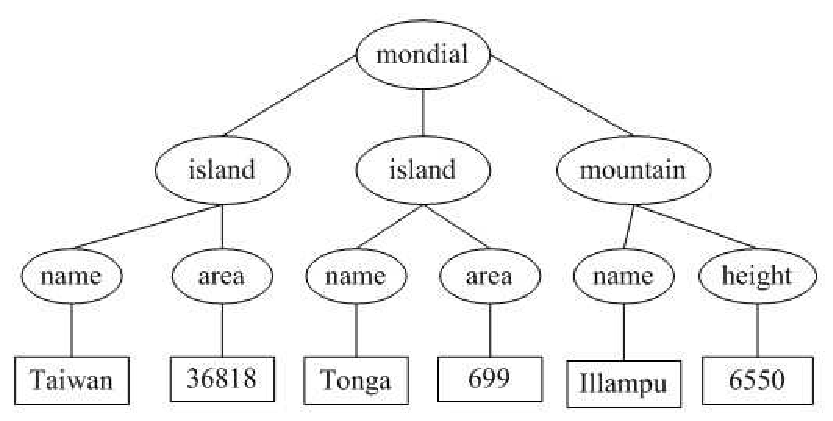
\includegraphics[width=0.4\textwidth]{XML}
\caption{树状结构}\label{fig:xml}
\vspace{\baselineskip}
\end{figure}


其插入图片的代码及其说明如下。
\vspace{1em}\noindent\hrule
\begin{verbatim}
\begin{figure}[htbp]
\centering
\includegraphics[width=0.4\textwidth]{文件名(.eps)}
\caption{标题}\label{标签名(通常为 fig:labelname)}
\vspace{\baselineskip} %表示图与正文空一行
\end{figure}
\end{verbatim}

\noindent\hrule

\begin{verbatim}
figure环境的可选参数[htbp]表示浮动图形所放置的位置,h (here)表示当前位置,t (top)表示页芯顶部,b (bottom)表示页芯底部,p (page)表示单独一页。在Word等软件中,图片通常插入到当前位置,如果当前页的剩余空间不够,图片将被移动到下一页,当前页就会出现很大的空白,其人工调整工作非常不便。由LaTeX提供的浮动图片功能,总是会按h->t->b->p的次序处理选项中的字母,自动调整图片的位置,大大减轻了工作量。
\centering命令将后续内容转换成每行皆居中的格式。
"\includegraphics"的可选参数用来设置图片插入文中的水平宽度,一般表示为正文宽度(\textwidth)的倍数。
\caption命令可选参数“标签名”为英文形式,一般不以图片或表格的数字顺序作为标签,而应包含一定的图片或表格信息,以便于文中引用(若图片、表格、公式、章节和参考文献等在文中出现的先后顺序发生了变化,其标注序号及其文中引用序号也会跟着发生变化,这一点是Word等软件所不能做到的)。另外,图题或表题并不会因为分页而与图片或表格体分置于两页,章节等各级标题也不会置于某页的最底部,LaTeX系统会自动调整它们在正文中的位置,这也是Word等软件所无法匹敌的。
\vspace将产生一定高度的竖直空白,必选参数为负值表示将后续文字位置向上提升,参数值可自行调整。em为长度单位,相当于大写字母M的宽度。\vspace{\baselineskip} 表示图与正文空一行。
引用方法:“见图~\ref{fig:figname}”、“如图~\ref{fig:figname}~所示”等。
\end{verbatim}

\noindent\hrule\vspace{1em}

若需要将~2~张及以上的图片并排插入到一行中,则需要采用\verb|minipage|环境,如图~\ref{fig:dd}~和图~\ref{fig:ds}~所示。
\begin{figure}[htbp]
\centering
\begin{minipage}{0.4\textwidth}
\centering
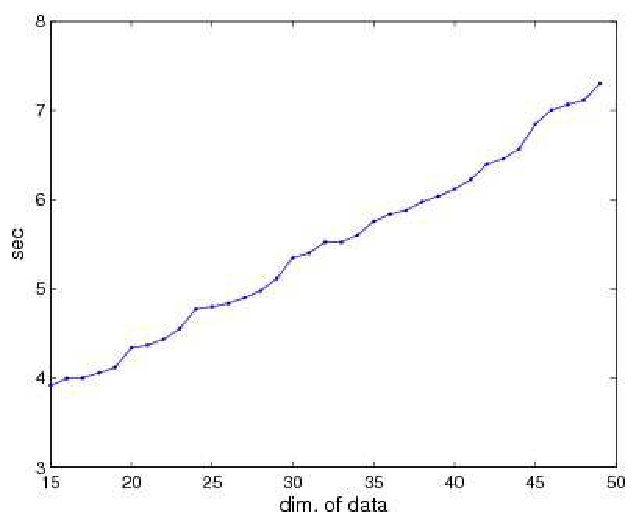
\includegraphics[width=\textwidth]{dataDimensions}
\caption{数据维数的变化}\label{fig:dd}
\end{minipage}
\begin{minipage}{0.4\textwidth}
\centering
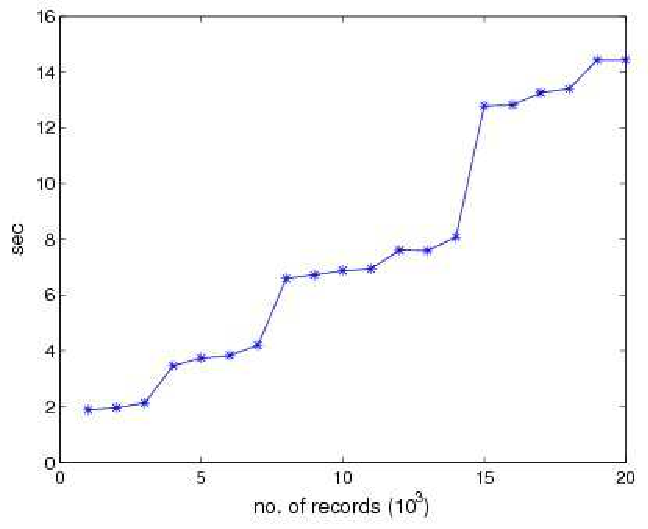
\includegraphics[width=\textwidth]{dataSize}
\caption{数据规模的变化}\label{fig:ds}
\end{minipage}
\vspace{\baselineskip}
\end{figure}

其代码如下所示。
\vspace{1em}\noindent\hrule
\begin{verbatim}
\begin{figure}[htbp]
\centering
\begin{minipage}{0.4\textwidth}
\centering
\includegraphics[width=\textwidth]{文件名}
\caption{标题}\label{fig:f1}
\end{minipage}
\begin{minipage}{0.4\textwidth}
\centering
\includegraphics[width=\textwidth]{文件名}
\caption{标题}\label{fig:f2}
\end{minipage}\vspace{\baselineskip}
\end{figure}
\end{verbatim}

\noindent\hrule

\begin{verbatim}
minipage环境的必选参数用来设置小页的宽度,若需要在一行中插入n个等宽图片,则每个小页的宽度应略小于(1/n)\textwidth。
\end{verbatim}

\noindent\hrule

\section{具有子图的图片插入方法}

图中若含有子图时,需要调用~subfigure~宏包, 如图~\ref{fig:subfig}~所示。
\begin{figure}[htbp]
  \centering
  \subfigure[Data Dimensions]{\label{fig:subfig:datadim}
                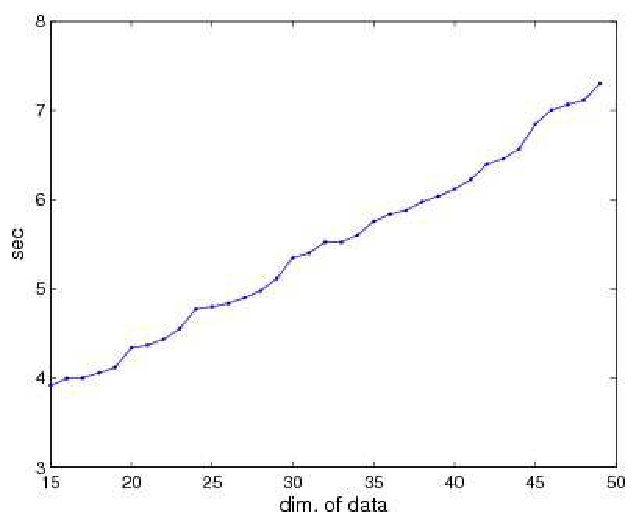
\includegraphics[width=0.4\textwidth]{dataDimensions}}
  \subfigure[Data Size]{\label{fig:subfig:datasize}
                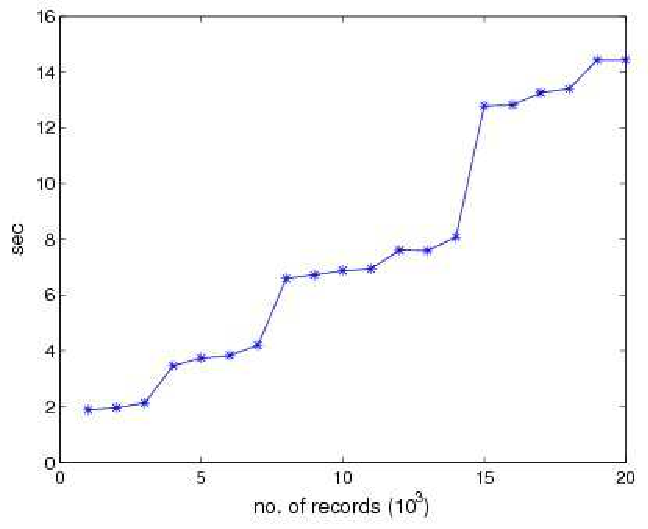
\includegraphics[width=0.4\textwidth]{dataSize}}
  \caption{Scalability of data}\label{fig:subfig}
\vspace{\baselineskip}
\end{figure}

其代码及其说明如下。
\vspace{1em}\noindent\hrule

\begin{verbatim}
\begin{figure}[htbp]
  \centering
  \subfigure[第1个子图标题]{
            \label{第1个子图标签(通常为 fig:subfig1:subsubfig1)}
            \includegraphics[width=0.4\textwidth]{文件名}}
  \subfigure[第2个子图标题]{
            \label{第2个子图标签(通常为 fig:subfig1:subsubfig2)}
            \includegraphics[width=0.4\textwidth]{文件名}}
  \caption{总标题}\label{总标签(通常为 fig:subfig1)}
\vspace{\baselineskip}
\end{figure}
\end{verbatim}

\noindent\hrule

\begin{verbatim}
子图的标签实际上可以随意设定,只要不重复就行。但为了更好的可读性,我们建议fig:subfig:subsubfig格式命名,这样我们从标签名就可以知道这是一个子图引用。
引用方法:总图的引用方法同本章第1节,子图的引用方法用\ref{fig:subfig:subsubfig}来代替。
\end{verbatim}

\noindent\hrule\vspace{1em}

子图的引用示例:如图~\ref{fig:subfig:datadim}~和图~\ref{fig:subfig:datasize}~所示。

若想获得插图方法的更多信息,参见网络上的~\href{ftp://ftp.tex.ac.uk/tex-archive/info/epslatex.pdf}{Using Imported Graphics in \LaTeX and pdf\LaTeX}~文档。 

\section{插入算法}

\begin{algorithm}[!h]
{
{
\renewcommand\baselinestretch{1.5}\selectfont %控制行距
\caption{ Scheduling Algorithm }
\label{alg:schedule}
\begin{algorithmic}[1]
\REQUIRE ~\\
A DFG $G=<V,E>$;\\
An allocation $A(G)$ for $G$.
\ENSURE ~\\
A schedule.
    \STATE{.......................}
    \FOR{$i\leftarrow\ 1\ to\ M$}    
        \STATE{.......................}
    \ENDFOR
    \STATE{.......................}
    \STATE{.......................}
    \STATE{.......................}
    \STATE{.......................}
    \STATE{.......................}
    \FOR{$k\leftarrow\ 1\ to\ |V|$}
        \STATE{.......................}
        \STATE{.......................}
        \STATE{.......................}
        \STATE{.......................}
    \IF{$LT_k==j$}
        \IF{there is no idle core in cluster $cl_{loc}$}
            \STATE{.......................}
            \STATE{.......................}
            \STATE{.......................}
            \STATE{.......................}
            \STATE{.......................}
            \STATE{.......................}
        \ELSE
            \STATE{.......................}
            \STATE{.......................}
            \STATE{.......................}
            \STATE{.......................}
            \STATE{.......................}
            \STATE{.......................}
        \ENDIF
    \ENDIF
    \ENDFOR
 

\end{algorithmic}
}
\par}
\end{algorithm}
%%% !Mode:: "TeX:UTF-8"

\chapter{表格的绘制方法}
\section{研究生毕业设计论文的绘表规范}

表应有自明性。表格不加左、右边线。表的编排建议采用国际通行的三线表。表内中文书写使用宋体五号字。

每个表格之上均应有表题(由表序和表名组成)。表序一般按章编排,如第~1~章第一个插表的序号为“表~1-1”等。表序与表名之间空两格,
表名使用中文五号字,居中。表名中不允许使用标点符号,表名后不加标点。
表头设计应简单明了,尽量不用斜线。表头中可采用化学,物理量等专业符号。

全表如用同一单位,则将单位符号移至表头右上角,加圆括号\cite{djy}。
表中数据应准确无误,书写清楚。数字空缺的格内加横线“-”(占~2~个数字宽度)。表内文字或数字上、下或左、右相同时,
采用通栏处理方式,不允许用“〃”、“同上”之类的写法。

表内文字使用宋体五号字,垂直居中书写,起行空一格、转行顶格、句末不加标点。
如某个表需要转页接排,在随后的各页上应重复表的编号。编号后加“(续表)”,表题可省略。续表应重复表头。
表格绘制完成之后,与正文空一行。

\section{普通表格的绘制方法}

表格应具有三线表格式,因此需要调用~booktabs~宏包,其标准格式如表~\ref{tab:table1}~所示。

\renewcommand\arraystretch{1.5}%控制行距
\begin{table}[!h]
\caption{基准测试集参数}\label{tab:bench}
\vspace{0.5em}
\centering
\begin{tabular}{l*{1}{C{2cm}}*{1}{L{6.2cm}}}
\toprule
Name         & $n$ & Description\\
\midrule
Random1      & 50  & Random graph generated by TGFF\\
Random2      & 100 & Random graph generated by TGFF\\
Random3      & 150 & Random graph generated by TGFF\\
Random4      & 200 & Random graph generated by TGFF\\
Random5      & 250 & Random graph generated by TGFF\\
Random6      & 300 & Random graph generated by TGFF\\
Random7      & 350 & Random graph generated by TGFF\\
Random8      & 400 & Random graph generated by TGFF\\
Random9      & 450 & Random graph generated by TGFF\\
Random10     & 500 & Random graph generated by TGFF\\
\bottomrule
\end{tabular}
\vspace{\baselineskip}
\end{table}
\renewcommand\arraystretch{1}

其绘制表格的代码及其说明如下。
\vspace{1em}\noindent\hrule

\begin{verbatim}
\begin{table}[htbp]
\caption{表标题}\label{标签名(通常为 tab:tablename)}
\vspace{0.5em}\centering\wuhao
\begin{tabular}{cc...c}
\toprule[1.5pt]
表头第1个格   & 表头第2个格   & ... & 表头第n个格  \\
\midrule[1pt]
表中数据(1,1) & 表中数据(1,2) & ... & 表中数据(1,n)\\
表中数据(2,1) & 表中数据(2,2) & ... & 表中数据(2,n)\\
表中数据(3,1) & 表中数据(3,2) & ... & 表中数据(3,n)\\
表中数据(4,1) & 表中数据(4,2) & ... & 表中数据(4,n)\\
...................................................\\
表中数据(m,1) & 表中数据(m,2) & ... & 表中数据(m,n)\\
\bottomrule[1.5pt]
\end{tabular}
\vspace{\baselineskip}
\end{table}
\end{verbatim}

\noindent\hrule

\begin{verbatim}
table环境是一个将表格嵌入文本的浮动环境。
\wuhao命令将表格的字号设置为五号字(10.5pt),在绘制表格结束退出时,不需要将字号再改回为\xiaosi,正文字号默认为小四号字(12pt)。
tabular环境的必选参数由每列对应一个格式字符所组成:c表示居中,l表示左对齐,r表示右对齐,其总个数应与表的列数相同。此外,@{文本}可以出现在任意两个上述的列格式之间,其中的文本将被插入每一行的同一位置。表格的各行以\\分隔,同一行的各列则以&分隔。
\toprule、\midrule和\bottomrule三个命令是由booktabs宏包提供的,其中\toprule和\bottomrule分别用来绘制表格的第一条(表格最顶部)和第三条(表格最底部)水平线,\midrule用来绘制第二条(表头之下)水平线,且第一条和第三条水平线的线宽为1.5pt,第二条水平线的线宽为1pt。
引用方法:“如表~\ref{tab:tablename}~所示”。
\end{verbatim}

\noindent\hrule

\section{长表格的绘制方法}

长表格是当表格在当前页排不下而需要转页接排的情况下所采用的一种表格环境。若长表格仍按照普通表格的绘制方法来获得,
其所使用的\verb|table|浮动环境无法实现表格的换页接排功能,表格下方过长部分会排在表格第1页的页脚以下。为了能够实现长表格的转页接排功能,
需要调用~longtable~宏包,由于长表格是跨页的文本内容,因此只需要单独的\verb|longtable|环境,所绘制的长表格的格式如表~\ref{tab:table2}~所示。

此长表格~\ref{tab:table2}~第~2~页的标题“编号(续表)”和表头是通过代码自动添加上去的,无需人工添加,若表格在页面中的竖直位置发生了变化,长表格在第~2~页
及之后各页的标题和表头位置能够始终处于各页的最顶部,也无需人工调整,\LaTeX~系统的这一优点是~Word~等软件所无法企及的。

下段内容是为了让下面的长表格分居两页,看到表标题“编号(续表)”的效果。摘录于《你若安好,便是晴天 -- 林徽因传》片段:

她叫林徽因,出生于杭州,是许多人梦中期待的白莲。她在雨雾之都伦敦,发生过一场空前绝后的康桥之恋。她爱过三个男子,爱得清醒,也爱得平静。徐志摩为她徜徉在康桥,深情地等待一场旧梦可以归来。梁思成与她携手走过千山万水,为完成使命而相约白头。金岳霖为她终身不娶,痴心不改地守候一世。可她懂得人生飘忽不定,要学会随遇而安。
真正的平静,不是避开车马喧嚣,而是在心中修篱种菊。尽管如流往事,每一天都涛声依旧,只要我们消除执念,便可寂静安然。愿每个人在纷呈世相中不会迷失荒径,可以端坐磐石上,醉倒落花前。
如果可以,请让我预支一段如莲的时光,哪怕将来某一天加倍偿还。这个雨季会在何时停歇,无从知晓。但我知道,你若安好,便是晴天。					
\wuhao\begin{longtable}{ccc}
\caption{湖南大学各学院名称一览}\label{tab:table2}
 \vspace{0.5em}\\
\toprule[1.5pt] 学院名称 & 网址 & 联系电话  \\ \midrule[1pt]
\endfirsthead
\multicolumn{3}{c}{表~\thetable(续表)}\vspace{0.5em}\\
\toprule[1.5pt] 学院名称 & 网址 & 联系电话  \\ \midrule[1pt]
\endhead
\bottomrule[1.5pt]
\endfoot
机械工程学院& \url{http://tdjxxy.tju.edu.cn/}& 87401979\\
精密仪器与光电子工程学院&  \url{http://www2.tju.edu.cn/colleges/precision/cn/}& 27404775\\
电子信息工程学院& \url{http://www.tju.edu.cn/seie}& 27406956\\
电气与自动化工程学院& \url{http://www2.tju.edu.cn/colleges/automate/}& 27405477\\
建筑工程学院& \url{http://www2.tju.edu.cn/colleges/civil/}& 27404072\\
化工学院& \url{http://chemeng.tju.edu.cn/}& 27403389\\
材料科学与工程学院& \url{http://mse.tju.edu.cn}& 27406693 \\
建筑学院& \url{http://hgw022072.chinaw3.com/}& 27402724-2111\\
求是学部\\
管理与经济学部&	\url{ http://sm.tju.edu.cn}& 27403423\\
理学院& \url{ http://www.tju.edu.cn/science/}& 27404118\\
文法学院& \url{ http://www2.tju.edu.cn/colleges/sociology/new/}& 27403691\\
软件学院& \url{http://scs.tju.edu.cn}& 87401540\\
计算机科学与技术学院& \url{http://cs.tju.edu.cn/}& 27406538\\
马克思主义学院& \url{http://www2.tju.edu.cn/colleges/marxism/}& 27405348\\
环境科学与工程学院& \url{http://www.tju.edu.cn/see}& 87402072\\
药物科学与技术学院& \url{http://www2.tju.edu.cn/colleges/pharmtier/}& 87401830\\
教育学院& \url{http://soe.tju.edu.cn/}& 27401028\\
职业技术教育学院& \url{http://202.113.0.248:8888}\\
继续教育学院& \url{http://aectu.tju.edu.cn/}& 27406298\\
仁爱学院& \url{http://www.tjrac.edu.cn/}& 68579990\\
农业与生物工程学院& \url{http://202.113.13.169/site/nongxueyuan/}& 87402171\\
国际教育学院 & \url{http://www.ietju.com/}& 27406147\\
网络教育学院 & \url{http://www.etju.com/}& 27426952 \\

\end{longtable}\xiaosi
\vspace{\baselineskip}

绘制长表格的代码及其说明如下。
\vspace{1em}\noindent\hrule

\begin{verbatim}
\wuhao\begin{longtable}{cc...c}
\caption{表标题}\label{标签名(通常为 tab:tablename)}\\
\toprule[1.5pt] 表头第1个格 & 表头第2个格 & ... & 表头第n个格\\ \midrule[1pt]
\endfirsthead
\multicolumn{n}{c}{表~\thetable(续表)}\vspace{0.5em}\\
\toprule[1.5pt] 表头第1个格 & 表头第2个格 & ... & 表头第n个格\\ \midrule[1pt]
\endhead
\bottomrule[1.5pt]
\endfoot
表中数据(1,1) & 表中数据(1,2) & ... & 表中数据(1,n)\\
表中数据(2,1) & 表中数据(2,2) & ... & 表中数据(2,n)\\
...................................................\\
表中数据(m,1) & 表中数据(m,2) & ... & 表中数据(m,n)\\
\end{longtable}\xiaosi
\end{verbatim}

\noindent\hrule
\begin{verbatim}
在绘制长表格的前面留出一个空白行,并在第2行的一开始全局定义长表格的字号为五号字,这样能够保证长表格之前段落的行距保持不变。
在绘制长表格结束后,需要\xiaosi命令重新将字号改为小四号字。
\endhead之前的文字描述的是第2页及其之后各页的标题或表头;
\endfirsthead之前的文字描述的是第1页的标题和表头,若无此命令,则第1页的表头和标题由\endhead命令确定;
同理,\endfoot之前的文字描述的是除最后一页之外每页的表格底部内容;
\endlastfoot之前的文字描述的是最后一页的表格底部内容,若无此命令,
则最后一页的表格底部内容由\endfoot命令确定;由于规范中长表格每页底部内容均相同(水平粗线),因此模板中没有用到\endlastfoot命令。
\end{verbatim}

\noindent\hrule
\section{列宽可调表格的绘制方法}
论文中能用到列宽可调表格的情况共有两种:一种是当插入的表格某一单元格内容过长以至于一行放不下的情况,
另一种是当对公式中首次出现的物理量符号进行注释的情况。这两种情况都需要调用~tabularx~宏包。下面将分别对这两种情况下可调表格的绘制方法进行阐述。
\subsection{表格内某单元格内容过长的情况}

首先给出这种情况下的一个例子如表~\ref{tab:table3}~所示。
\begin{table}[htbp]
\caption{最小的三个正整数的英文表示法}\label{tab:table3}
\vspace{0.5em}\wuhao
\begin{tabularx}{\textwidth}{llX}
\toprule[1.5pt]
Value & Name & Alternate names, and names for sets of the given size\\\midrule[1pt]
1 & One & ace, single, singleton, unary, unit, unity\\
2 & Two & binary, brace, couple, couplet, distich, deuce, double, doubleton, duad, duality, duet, duo, dyad, pair, snake eyes, span, twain, twosome, yoke\\
3 & Three & deuce-ace, leash, set, tercet, ternary, ternion, terzetto, threesome, tierce, trey, triad, trine, trinity, trio, triplet, troika, hat-trick\\\bottomrule[1.5pt]
\end{tabularx}
\vspace{\baselineskip}
\end{table}
绘制这种表格的代码及其说明如下。
\vspace{1em}\noindent\hrule
\begin{verbatim}
\begin{table}[htbp]
\caption{表标题}\label{标签名(通常为 tab:tablename)}
\vspace{0.5em}\wuhao
\begin{tabularx}{\textwidth}{l...X...l}
\toprule[1.5pt]
表头第1个格   & ... & 表头第X个格   & ... & 表头第n个格  \\
\midrule[1pt]
表中数据(1,1) & ... & 表中数据(1,X) & ... & 表中数据(1,n)\\
表中数据(2,1) & ... & 表中数据(2,X) & ... & 表中数据(2,n)\\
.........................................................\\
表中数据(m,1) & ... & 表中数据(m,X) & ... & 表中数据(m,n)\\
\bottomrule[1.5pt]
\end{tabularx}
\vspace{\baselineskip}
\end{table}
\end{verbatim}

\noindent\hrule
\begin{verbatim}
tabularx环境共有两个必选参数:第1个参数用来确定表格的总宽度,这里取为排版表格能达到的最大宽度——正文宽度\textwidth;第2个参数用来确定每列格式,其中标为X的项表示该列的宽度可调,其宽度值由表格总宽度确定。
标为X的列一般选为单元格内容过长而无法置于一行的列,这样使得该列内容能够根据表格总宽度自动分行。若列格式中存在不止一个X项,则这些标为X的列的列宽相同,因此,一般不将内容较短的列设为X。
标为X的列均为左对齐,因此其余列一般选为l(左对齐),这样可使得表格美观,但也可以选为c或r。
\end{verbatim}

\noindent\hrule
\subsection{对物理量符号进行注释的情况}
为使得对公式中物理量符号注释的转行与破折号“———”后第一个字对齐,此处最好采用表格环境。此表格无任何线条,左对齐,
且在破折号处对齐,一共有“式中”二字、物理量符号和注释三列,表格的总宽度可选为文本宽度,因此应该采用\verb|tabularx|环境。
由\verb|tabularx|环境生成的对公式中物理量符号进行注释的公式如式(\ref{eq:1})所示。
%\vspace*{10pt}

\begin{equation}\label{eq:1}
\ddot{\boldsymbol{\rho}}-\frac{\mu}{R_{t}^{3}}\left(3\mathbf{R_{t}}\frac{\mathbf{R_{t}\rho}}{R_{t}^{2}}-\boldsymbol{\rho}\right)=\mathbf{a}
\end{equation}

\begin{tabularx}{\textwidth}{@{}l@{\quad}r@{———}X@{}}
式中& $\bm{\rho}$ &追踪飞行器与目标飞行器之间的相对位置矢量;\\
&  $\bm{\ddot{\rho}}$&追踪飞行器与目标飞行器之间的相对加速度;\\
&  $\mathbf{a}$   &推力所产生的加速度;\\
&  $\mathbf{R_t}$ & 目标飞行器在惯性坐标系中的位置矢量;\\
&  $\omega_{t}$ & 目标飞行器的轨道角速度;\\
&  $\mathbf{g}$ & 重力加速度,$=\frac{\mu}{R_{t}^{3}}\left(
3\mathbf{R_{t}}\frac{\mathbf{R_{t}\rho}}{R_{t}^{2}}-\bm{\rho}\right)=\omega_{t}^{2}\frac{R_{t}}{p}\left(
3\mathbf{R_{t}}\frac{\mathbf{R_{t}\rho}}{R_{t}^{2}}-\bm{\rho}\right)$,这里~$p$~是目标飞行器的轨道半通径。
\end{tabularx}
\vspace{\wordsep}

其中生成注释部分的代码及其说明如下。

\vspace{1em}\noindent\hrule

\begin{verbatim}
\begin{tabularx}{\textwidth}{@{}l@{\quad}r@{— — —}X@{}}
式中 & symbol-1 & symbol-1的注释内容;\\
     & symbol-2 & symbol-2的注释内容;\\
     .............................;\\
     & symbol-m & symbol-m的注释内容。
\end{tabularx}\vspace{\wordsep}
\end{verbatim}

\noindent\hrule

\begin{verbatim}
tabularx环境的第1个参数选为正文宽度,第2个参数里面各个符号的意义为:
    第1个@{}表示在“式中”二字左侧不插入任何文本,“式中”二字能够在正文中左对齐,若无此项,则“式中”二字左侧会留出一定的空白;
    @{\quad}表示在“式中”和物理量符号间插入一个空铅宽度的空白;
    @{— — —}实现插入破折号的功能,它由三个1/2的中文破折号构成;
    第2个@{}表示在注释内容靠近正文右边界的地方能够实现右对齐。
\end{verbatim}

\noindent\hrule\vspace{1em}

由此方法生成的注释内容应紧邻待注释公式并置于其下方,因此不能将代码放入\verb|table|浮动环境中。但此方法不能实现自动转页接排,
可能会在当前页剩余空间不够时,全部移动到下一页而导致当前页出现很大空白。因此在需要转页处理时,还请您手动将需要转页的代码放入一个
新的\verb|tabularx|环境中,将原来的一个\verb|tabularx|环境拆分为两个\verb|tabularx|环境。

若想获得绘制表格的更多信息,参见网络上的~\href{http://www.tug.org/pracjourn/2007-1/mori/}{Tables in \LaTeXe: Packages and Methods}~文档。


%%% !Mode:: "TeX:UTF-8"

\chapter{数学公式的输入方法}
\section{研究生毕业设计论文的公式规范}

论文中的公式应另起行,原则上应居中书写,与周围文字留有足够的空间区分开。
若公式前有文字(如“解”、“假定”等),文字空两格写,公式仍居中写。公式末不加标点。

公式应标注序号,并将序号置于括号内。 公式序号按章编排,如第~1~章第一个公式序号为“(1-1)”。公式的序号右端对齐。

公式较长时最好在等号“=”处转行,如难实现,则可在~$+$、$-$、$\times$、$\div$~运算符号处转行,转行时运算符号仅书写于转行式前,不重复书写。

文中引用公式时,一般用“见式~(1-1)”或“由公式~(1-1)”。

公式中用斜线表示“除”的关系时应采用括号,以免含糊不清,如~$a/(b\cos x)$。通常“乘”的关系在前,如~$a\cos x/b$而不写成~$(a/b)\cos x$。

不能用文字形式表示等式,如:$\textnormal{刚度}=\frac{{\textnormal{受力}}}{{\textnormal{受力方向的位移}}}$。

对于数学公式的输入方法,网络上有一个比较全面权威的文档\textbf{~\href{http://tug.ctan.org/cgi-bin/ctanPackageInformation.py?id=voss-mathmode}{Math mode}}~请大家事先大概浏览一下。下面将对学位论文中主要用到的数学公式排版形式进行阐述。

\section{生成~\LaTeX~数学公式的两种方法}
对于先前没有接触过~\LaTeX~的人来说,编写~\LaTeX~数学公式是一件很繁琐的事,尤其是对复杂的数学公式来说,更可以说是一件难以完成的任务。
实际上,生成~\LaTeX~数学公式有两种较为简便的方法,一种是基于~MathType~数学公式编辑器的方法,另一种是基于~MATLAB~商业数学软件的方法,
下面将分别对这两种数学公式的生成方法作一下简单介绍。

\subsection{基于~MathType~软件的数学公式生成方法}
MathType~是一款功能强大的数学公式编辑器软件,能够用来在文本环境中插入~Windows OLE~图形格式的复杂数学公式,所以应用比较普遍。但此软件只有~30~天的试用期,之后若再继续使用则需要付费购买才行。网络上有很多破解版的~MathType~软件可供下载免费使用,
笔者推荐下载安装版本号在~6.5~之上的中文破解版。

在安装好~MathType~之后,若在输入窗口中编写数学公式,复制到剪贴板上的仍然是图形格式的对象。
若希望得到可插入到~\LaTeX~编辑器中的文本格式对象,则需要对~MathType~软件做一下简单的设置:在~MathType~最上排的按钮中依次选择“参数选项
$\to$转换”,在弹出的对话窗中选中“转换到其它语言(文字):”,在转换下拉框中选择“Tex~--~--~LaTeX 2.09 and later”,并将对话框最下方的两个复选框全部勾掉,点击确定,这样,再从输入窗口中复制出来的对象就是文本格式的了,就可以直接将其粘贴到~\LaTeX~
编辑器中了。按照这种方法生成的数学公式两端分别有标记\verb|\[|和标记\verb|\]|,在这两个标记之间才是真正的数学公式代码。

若希望从~MathType~输入窗口中复制出来的对象为图形格式,则只需再选中“公示对象(Windows OLE~图形)”即可。

\subsection{基于~MATLAB~软件的数学公式生成方法}

MATLAB~是矩阵实验室(Matrix Laboratory)的简称,是美国~MathWorks~公司出品的商业数学软件。它是当今科研领域最常用的应用软件之一,
具有强大的矩阵计算、符号运算和数据可视化功能,是一种简单易用、可扩展的系统开发环境和平台。

MATLAB~中提供了一个~latex~函数,它可将符号表达式转化为~\LaTeX~数学公式的形式。其语法形式为~latex(s),其中,~s~为符号表达式,
之后再将~latex~函数的运算结果直接粘贴到~\LaTeX~编辑器中。从~\LaTeX~数学公式中可以发现,其中可能包含如下符号组合:

\begin{verbatim*}
\qquad=两个空铅(quad)宽度
\quad=一个空铅宽度
\;=5/18空铅宽度
\:=4/18空铅宽度
\,=3/18空铅宽度
\!=-3/18空铅宽度
\ =一个空格
\end{verbatim*}

所以最好将上述符号组合从数学公式中删除,从而使数学公式显得匀称美观。

对于~Word~等软件的使用者来说,在我们通过~MATLAB~运算得到符号表达式形式的运算结果时,在~Word~中插入运算结果需要借助于~MathType~软件,
通过在~MathType~中输入和~MATLAB~运算结果相对应的数学表达形式,之后再将~MathType~数学表达式转换为图形格式粘贴到~Word~中。实际上,
也可以将~MATLAB~中采用~latex~函数运行的结果直接粘贴到~MathType~中,再继续上述步骤,这样可以大大节省输入公式所需要的时间。
此方法在~MathType~6.5c~上验证通过,若您粘入到~MathType~中的仍然为从~MATLAB~中导入的代码,请您更新~MathType~软件。

\section{数学字体}
在数学模式下,常用的数学字体命令有如下几种:

\begin{verbatim}
\mathnormal或无命令 用数学字体打印文本;
\mathit             用斜体(\itshape)打印文本;
\mathbf             用粗体(\bfseries)打印文本;
\mathrm             用罗马体(\rmfamily)打印文本;
\mathsf             用无衬线字体(\sffamily)打印文本;
\mathtt             用打印机字体(\ttfamily)打印文本;
\mathcal            用书写体打印文本;
\end{verbatim}

在学位论文撰写中,只需要用到上面提到的~\verb|\mathit|、\verb|\mathbf|~和~\verb|\mathrm|~命令。若要得到~Times New Roman~的数学字体,则需要调用~txfonts~宏包(此宏包实际上采用的是~Nimbus Roman No9 L~字体,
它是开源系统中使用的免费字体,其字符字体与~Times New Roman~字体几乎完全相同);若要得到粗体数学字体,则需要调用~bm~宏包。表~\ref{tab:fonts}~中分别列出了得到阿拉伯数字、拉丁字母和希腊字母
各种数学字体的命令。

\begin{table}[htbp]
\caption{常用数学字体命令一览}\label{tab:fonts}
\vspace{0.5em}\centering\wuhao
\begin{tabular}{llll}
\toprule
 & 阿拉伯数字\&大写希腊字母 & 大小写拉丁字母 & 小写希腊字母  \\
\midrule
斜体 & \verb|\mathit{}| & \verb|无命令| & \verb|无命令|\\
粗斜体 & \verb|\bm{\mathit{}}| & \verb|\bm{}| & \verb|\bm{}|\\
直立体 & \verb|无命令| & \verb|\mathrm{}| & \verb|字母后加up|\\
粗体 & \verb|\mathbf{}或\bm{}| & \verb|\mathbf{}| & \verb|\bm{字母后加up}|\\
\bottomrule
\end{tabular}
\vspace{\baselineskip}
\end{table}

\noindent 下面列出了一些应采用直立数学字体的数学常数和数学符号。

\vspace{-0.5em}\begin{center}\begin{tabularx}{0.7\textwidth}{XX}
$\mathrm{d}$、 $\mathrm{D}$、 $\mathrm{p}$~———微分算子 & $\mathrm{e}$~———自然对数之底数\\
$\mathrm{i}$、 $\mathrm{j}$~———虚数单位 & $\piup$———圆周率\\
\end{tabularx}\end{center}

\section{行内公式}
出现在正文一行之内的公式称为行内公式,例如~$f(x)=\int_{a}^{b}\frac{\sin{x}}{x}\mathrm{d}x$。对于非矩阵和非多行形式的行内公式,一般不会使得行距发生变化,而~Word~等软件却会根据行内公式的竖直距离而自动调节行距,如图~\ref{fig:hangju}~所示。

\begin{figure}[htbp]
\centering
\subfigure[由~\LaTeX~系统生成的行内公式]{\label{fig:subfig:latex}
                \fbox{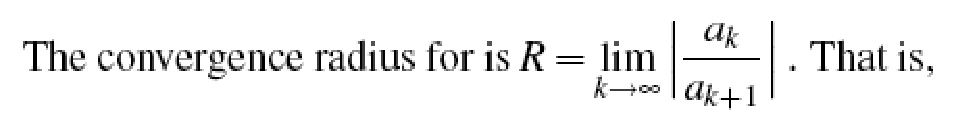
\includegraphics[width=0.55\textwidth]{latex}}}
\subfigure[由~Word软件生成的~.doc~格式行内公式]{\label{fig:subfig:word}
                \fbox{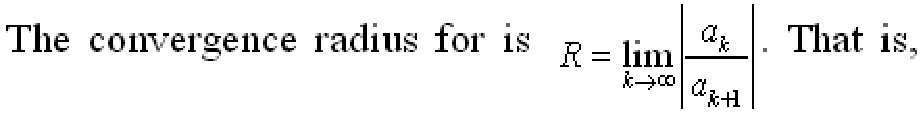
\includegraphics[width=0.55\textwidth]{word}}}
\subfigure[由~Word软件生成的~.pdf~格式行内公式]{\label{fig:subfig:pdf}
                \fbox{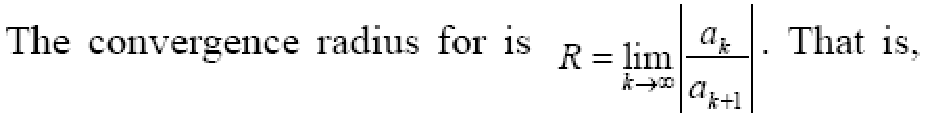
\includegraphics[width=0.55\textwidth]{pdf}}}

\caption{由~\LaTeX~和~Word~生成的~3~种行内公式屏显效果}\label{fig:hangju}
\vspace{-1em}
\end{figure}

这三幅图分别为~\LaTeX~和~Word~生成的行内公式屏显效果,从图中可看出,在~\LaTeX~文本含有公式的行内,在正文与公式之间对接工整,行距不变;而在~Word~文本含有公式的行内,在正文与公式之间对接不齐,行距变大。因此从这一点来说,
\LaTeX~系统在数学公式的排版上具有很大优势。

\LaTeX~提供的行内公式最简单、最有效的方法是采用~\TeX~本来的标记———开始和结束标记都写作~\$,例如本段开始的例子可由下面的输入得到。
\verb|$f(x)=\int_{a}^{b}\frac{\sin{x}}{x}\mathrm{d}x$|

\section{行间公式}
位于两行之间的公式称为行间公式,每个公式都是一个单独的段落,例如
\[\int_a^b{f\left(x\right)\mathrm{d}x}=\lim_{\left\|\Delta{x_i}\right\|\to 0}\sum_i{f\left(\xi_i\right)\Delta{x_i}}\]
除人工编号外,\LaTeX~各种类型行间公式的标记见表~\ref{tab:eqtag}。
\begin{table}[htbp]
\caption{各种类型行间公式的标记}\label{tab:eqtag}
\vspace{0.5em}\centering\wuhao
\begin{tabularx}{\textwidth}{cll}
\toprule
& 无编号 & 自动编号\\
\midrule
单行公式& \verb|\begin{displaymath}... \end{displaymath}|& \verb|\begin{equation}... \end{equation}|\\
        & 或~\verb|\[...\]| & \\
多行公式& \verb|\begin{eqnarray*}... \end{eqnarray*}|& \verb|\begin{eqnarray}... \end{eqnarray}|\\
\bottomrule
\end{tabularx}
\end{table}

另外,在自动编号的某行公式行尾添加标签~\verb|\nonumber|,可将该行转换为无编号形式。

行间多行公式需采用~\verb|eqnarray|~或~\verb|eqnarray*|~环境,它默认是一个列格式为~\verb|rcl|~的~3~列矩阵,并且中间列的字号要小一些,因此通常只将需要对齐的运算符号(通常为等号“=”)置于中间列。

\section{可自动调整大小的定界符}
若在左右两个定界符之前分别添加命令~\verb|\left|~和~\verb|\right|,则定界符可根据所包围公式大小自动调整其尺寸,这可从式(\ref{nodelimiter})和式(\ref{delimiter})中看出。
\begin{equation}\label{nodelimiter}
(\sum_{k=\frac12}^{N^2})
\end{equation}
\begin{equation}\label{delimiter}
\left(\sum_{k=\frac12}^{N^2}\right)
\end{equation}
式(\ref{nodelimiter})和式(\ref{delimiter})是在~\LaTeX~中分别输入如下代码得到的。
\begin{verbatim}
(\sum_{k=\frac12}^{N^2})
\left(\sum_{k=\frac12}^{N^2}\right)
\end{verbatim}
\verb|\left|~和~\verb|\right|~总是成对出现的,若只需在公式一侧有可自动调整大小的定界符,则只要用“.”代替另一侧那个无需打印出来的定界符即可。

若想获得关于此部分内容的更多信息,可参见~\href{http://tug.ctan.org/cgi-bin/ctanPackageInformation.py?id=voss-mathmode}{Math mode}~文档的第~8~章“Brackets, braces and parentheses”。

\section{数学重音符号}
数学重音符号通常用来区分同一字母表示的不同变量,输入方法如下(需要调用~\verb|amsmath|~宏包):

\vspace{0.5em}\noindent\wuhao\begin{tabularx}{\textwidth}{Xc|Xc|Xc}
 \verb|\acute| & $\acute{a}$ & \verb|\mathring| & $\mathring{a}$ & \verb|\underbrace| & $\underbrace{a}$ \\
 \verb|\bar| & $\bar{a}$ & \verb|\overbrace| & $\overbrace{a}$ & \verb|\underleftarrow| & $\underleftarrow{a}$ \\
 \verb|\breve| & $\breve{a}$ & \verb|\overleftarrow| & $\overleftarrow{a}$ & \verb|\underleftrightarrow| & $\underleftrightarrow{a}$ \\
 \verb|\check| & $\check{a}$ & \verb|\overleftrightarrow| & $\overleftrightarrow{a}$ & \verb|\underline| & $\underline{a}$ \\
 \verb|\dddot| & $\dddot{a}$ & \verb|\overline| & $\overline{a}$ & \verb|\underrightarrow| & $\underrightarrow{a}$ \\
 \verb|\ddot| & $\ddot{a}$ & \verb|\overrightarrow| & $\overrightarrow{a}$ & \verb|\vec| & $\vec{a}$ \\
 \verb|\dot| & $\dot{a}$ & \verb|\tilde| & $\tilde{a}$ & \verb|\widehat| & $\widehat{a}$ \\
 \verb|\grave| & $\grave{a}$ & \verb|\underbar| & $\underbar{a}$ & \verb|\widetilde| & $\widetilde{a}$ \\
 \verb|\hat| & $\hat{a}$
\end{tabularx}\vspace{0.5em}
\xiaosi 当需要在字母~$i$~和~$j$~的上方添加重音符号时,为了去掉这两个字母顶上的小点,这两个字母应该分别改用~\verb|\imath|~和~\verb|\jmath|。

如果遇到某些符号不知道该采用什么命令能输出它时,则可通过~\href{http://detexify.kirelabs.org/classify.html}{Detexify$^2$~网站}来获取符号命令。若用鼠标左键在此网页的方框区域内画出你所要找的符号形状,则会在网页右方列出和你所画符号形状相近的~5~个符号及其相对应的~\LaTeX~输入命令。若所列出的符号中不包括你所要找的符号,还可通过点击“Select from the complete list!”的链接以得分从低到高的顺序列出所有符号及其相对应的~\LaTeX~输入命令。

最后,建议大家还以~\href{http://tug.ctan.org/cgi-bin/ctanPackageInformation.py?id=voss-mathmode}{Math mode}~这篇~pdf~文档作为主要参考。若要获得最为标准、美观的数学公式排版形式,可以查查文档中是否有和你所要的排版形式相同或相近的代码段,通过修改代码段以获得你所要的数学公式排版形式。


%%% !Mode:: "TeX:UTF-8"

\chapter{罗列和定理环境使用方法}

\section{单层罗列环境}
湖南大学学位论文一般可采用两种罗列环境:一种是并列条目有同样标签的~\verb|itemize|~罗列环境,另一种是具有自动排序编号符号的~\verb|enumerate|~罗列环境。这两种罗列环境的样式参数可参考图~\ref{fig:list}。
\begin{figure}[htbp]
\centering
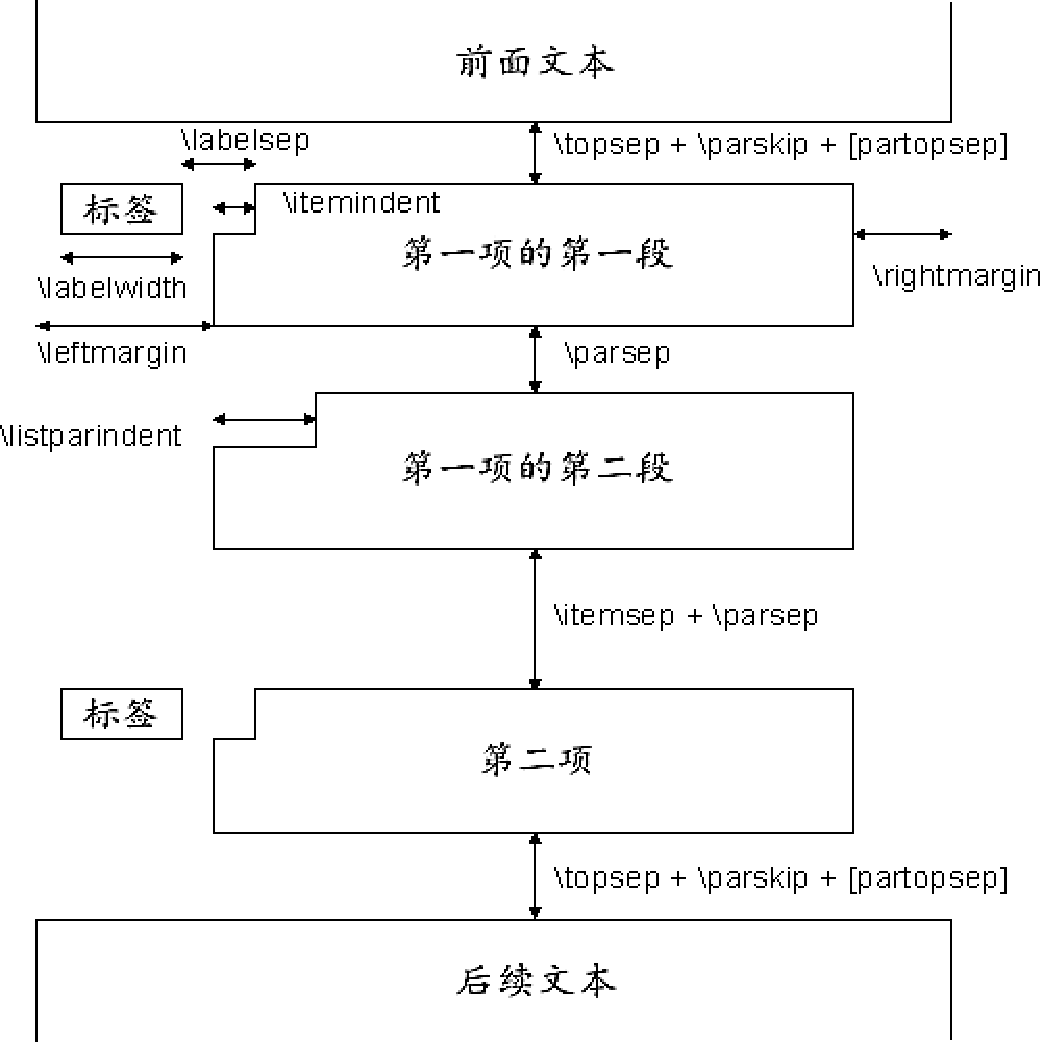
\includegraphics[width = 0.6\textwidth]{list}
\caption{罗列环境参数示意图}\label{fig:list}\vspace{-1em}
\end{figure}

通过调用~enumitem~宏包可以很方便地控制罗列环境的布局,其~format.tex~文件中的~\verb|\setitemize|~和~\verb|\setenumerate|~命令分别用来设置~\verb|itemize|~和~\verb|enumerate|~环境的样式参数。采用~\verb|itemize|~单层罗列环境的排版形式如下:

\begin{itemize}
\item 第一个条目文本内容
\item 第二个条目文本内容
\item 第三个条目文本内容
\end{itemize}

其代码如下

\begin{verbatim}
\begin{itemize}
  \item 第一个条目文本内容
  \item 第二个条目文本内容
  ...
  \item 第三个条目文本内容
\end{itemize}
\end{verbatim}

采用~\verb|enumerate|~单层罗列环境的排版形式如下:

\begin{enumerate}
\item 第一个条目文本内容
\item 第二个条目文本内容
\item 第三个条目文本内容
\end{enumerate}

其代码如下

\begin{verbatim}
\begin{enumerate}
  \item 第一个条目文本内容
  \item 第二个条目文本内容
  ...
  \item 第三个条目文本内容
\end{enumerate}
\end{verbatim}



\section{定理环境}

\begin{definition}[谱半径]\label{def:def1}
  称~$n$~阶方阵~$\mathbf{A}$~的全体特征值~$\lambda_1,\cdots,\lambda_n$~组成的集合为~$\mathbf{A}$~的谱,称
  $$\rho(\mathbf{A})=\max{\{|\lambda_1|,\cdots,|\lambda_n|\}}$$
\end{definition}
\begin{theorem}[相似充要条件]\label{lemma:l1}
  方阵$A$和$B$相似的充要条件是:~$A$~和~$B$~有全同的不变因子。
\end{theorem}
\begin{corollary}[推论1]\label{cor:cor1}
在赋范空间~$(X,\|\cdot\|)$~上定义~$d(x,y)=\|x-y\|$, 对任意~$x,y\in X$,~则~$(X,d)$~是距离空间。
\end{corollary}
\begin{proof}
  只需证明~$d(x,y)$~是距离。
\end{proof}
\newpage

定义代码如下:
\begin{verbatim}
 \begin{definition}[谱半径]\label{def:def1}
  称~$n$~阶方阵~$\mathbf{A}$~的全体特征值
  $\lambda_1,\cdots,\lambda_n$组成的集合为~$\mathbf{A}$~的谱,称
  $$\rho(\mathbf{A})=\max{\{|\lambda_1|,\cdots,|\lambda_n|\}}$$
\end{definition}
\end{verbatim}
\noindent\hrule

\vspace{0.1em}\noindent\hrule
\vspace{1em}
定理代码如下:
\begin{verbatim}
\begin{theorem}[相似充要条件]\label{lemma:l1}
  方阵$A$和$B$相似的充要条件是:$A$和$B$有全同的不变因子。
\end{theorem}
\end{verbatim}
\noindent\hrule\vspace{0.1em}

\noindent\hrule
\vspace{1em}
推论和证明代码如下:
\begin{verbatim}
\begin{corollary}[推论1]\label{cor:cor1}
在赋范空间~$(X,\|\cdot\|)$~上定义$d(x,y)=\|x-y\|$,
对任意$x,y\in X$,则$(X,d)$是距离空间。
\end{corollary}
\begin{proof}
  只需证明$d(x,y)$是距离。
\end{proof}
\end{verbatim}
\noindent\hrule\vspace{1em}

定理定义[]中是可选参数,用来说明定理的名称。其他环境格式书写与上面定理、定义、推论格式相同,可自己调用其他环境。
若需要书写定理定义等内容,而且带有顺序编号,需要采用如下环境。除了~\verb|proof|~环境之外,其余~9~个环境都可以有一个可选参数作为附加标题。

\begin{center}
\vspace{0.5em}\noindent\wuhao\begin{tabularx}{0.7\textwidth}{lX|lX}
定理 & \verb|theorem|~环境 & 定义 & \verb|definition|~环境 \\
例 & \verb|example|~环境 & 算法 & \verb|algorithm|~环境 \\
公理 & \verb|axiom|~环境 & 命题 & \verb|proposition|~环境 \\
引理 & \verb|lemma|~环境 & 推论 & \verb|corollary|~环境 \\
注解 & \verb|remark|~环境 & 证明 & \verb|proof|~环境 \\
\end{tabularx}
\end{center} 
%%\section{conclusion}
\label{sec:conclusion}
%\del{In this paper, we have proved the Min-Min  SRLG-Disjoint routing problem is NP-complete.}
In this paper, we propose an efficient algorithm to solve the Min-Min  SRLG-Disjoint routing problem in the presence of the trap problem. To reduce the complexity of searching for the alternative pair, we propose a divide-and-conquer solution to partition the original Min-Min SRLG-Disjoint routing problem into multiple sub-problems based on a SRLG conflicting link set derived from the AP path encountering the trap problem. Our algorithm takes advantage of existing AP search results and parallel executions for significantly faster path finding.
We have conducted extensive simulations  using the topology trace  on a multi-core CPU platform. The simulation results demonstrate that our algorithm can outperform other approaches with higher routing performance while at a much higher search speed.

\end{verbatim}
那么,编译的时候就只编译未加~\%~的一章,在这个例子中,即本章~intros。

理论上,并不一定要把每章放在不同的文件中。但是这种自顶向下,分章节写作、编译的方法有利于提高效率,大大减少~Debug~过程中的编译时间,同时减小风险。

\section{参考文献生成方法}

\LaTeX~具有插入参考文献的能力。Google Scholar~网站上存在兼容~BibTeX~的参考文献信息,通过以下几个步骤,可以轻松完成参考文献的生成。
\begin{itemize}
  \item 在\href{http://scholar.google.com/}{谷歌学术搜索}中,
        点击\href{http://scholar.google.com/scholar_preferences?hl=en&as_sdt=0,5}{学术搜索设置}。
  \item 页面打开之后,在\textbf{文献管理软件}选项中选择\textbf{显示导入~BibTeX~的链接},单击保存设置,退出。
  \item 在谷歌学术搜索中检索到文献后,在文献条目区域单击导入~BibTeX~选项,页面中出现文献的引用信息。
  \item 将文献引用信息的内容复制之后,添加到~references~文件夹下的~reference.bib~中。
\end{itemize}

\section{编译注意事项}
\begin{enumerate}
  \item 由于模板使用~UTF-8~编码,所以源文件应该保存成~UTF-8~格式,否则可能出现中文字符无法识别的错误。
  本模板中每一个~.tex~文件的文件的开头已经加上一行:\\
    \verb|% !Mode:: "TeX:UTF-8"|\\
     这样可以确保~.tex~文件默认使用~UTF-8~的格式打开。读者如果删去此行,很有可能会导致中文字符显示乱码。
     在~WinEdt~编辑器中可以使用以下两种方式保存成~UTF-8~格式:
      \begin{enumerate}
        \item 先建立~.tex~文件,另存为~.tex~文件时,选择用~UTF-8~格式保存。
        \item
            在~WinEdt~编辑器中,选择\\
            \mbox{~Document$\to$Document Settings$\to$Document Mode $\to$TeX:UTF-8} 同时在~WinEdt~最下面的状态栏中,可以看到该文档是~TeX~格式还是~TeX:UTF-8~格式。
            当文档为~TeX:UTF-8~格式时,状态栏一般显示:
            \makebox[\textwidth][l]{Wrap | Indent | INS | LINE |Spell | TeX:UTF-8 | -src~等。}
      \end{enumerate}
  \item 如果在pdf书签中,中文显示乱码的话,则注意以下说明:
    \begin{verbatim}
        \usepackage{CJKutf8}
        % 1. 如果使用CJKutf8
        %    Hyperref中应使用unicode参数
        % 2. 如果使用CJK
        %    Hyperref则使用CJKbookmarks参数
        %    可惜得到的PDF书签是乱码,建议弃用
        % 3. Unicode选项和CJKbookmarks不能同时使用
        \usepackage[
        %CJKbookmarks=true,
        unicode=true
        ]{hyperref}
     \end{verbatim}
 \item 建议采用以下两种编译方式:
  \begin{enumerate}
     \item latex + bibtex + latex + latex + dvi2pdf. 在这种编译情况下,对应的~hnumain.tex~文件的第一行是\verb|\def\usewhat{dvipdfmx}|~(缺省设置)。 此时,所有图片文件应该保存为~.eps~格式,如~figures~文件夹里~.eps~图片。
          如果您选择在命令行中操作,可以在编译的时候依次输入~latex hnumain, bibtex hnumain, latex hnumain, latex hnumain~和~dvipdfmx hnumain, 编译完成之后,需要手动打开~pdf~文件。
     \item pdflatex + pdflatex. 在这种编译情况下,对应的~hnumain.tex~文件的第一行应该改为\verb|\def\usewhat{pdflatex}|~。 此时, 编译不支持~.eps~图片格式,此时需要在命令行下使用~epstopdf~指令将~figures~文件夹下 的~.eps~文件转化成~.pdf~文件格式,命令行中操作格式为~epstopdf a.eps~。
          在命令行编译的时候,依次输入~pdflatex hnumain~和~pdflatex hnumain, 编译完成之后,需要手动打开~pdf~文件。
  \end{enumerate}
\end{enumerate}

\section{系统要求}
    CTEX 2.8, MiKTeX 2.8, TeX Live 2009~或以上版本。使用推荐的~WinEdt 6.0~编辑器,可以完成文件的编辑和编译工作。

\section{\TeX~简介}

以下内容是~milksea@bbs.ctex.org~撰写的关于~\TeX~的简单介绍,略有改动。
注意这不是一个入门教程,不讲~\TeX~系统的配置安装,也不讲具体的~\LaTeX~代码。
这里仅仅试图以一些只言片语来解释:
进入这个门槛之前新手应该知道的注意事项,以及遇到问题以后该去如何解决问题。

\subsection{什么是 \TeX/\LaTeX,我是否应该选择它~?}

\TeX~是最早由高德纳(Donald Knuth)教授创建的一门标记式宏语言,
用来排版科技文章,尤其擅长处理复杂的数学公式。\TeX~同时也是处理这一语言的排版软件。
\LaTeX~是 Leslie Lamport 在~\TeX~基础上按内容/格式分离和模块化等思想建立的一集~\TeX~上的格式。

\TeX~本身的领域是专业排版领域
但现在~TeX/LaTeX~也被广泛用于生成电子文档甚至幻灯片等,~\TeX~语言的数学部分
偶尔也在其他一些地方使用。但注意~\TeX~并不适用于文书处理(Microsoft Office 的领域,以前和现在都不是)。

选择使用~\TeX/\LaTeX~的理由包括:
\begin{itemize}
\item 免费软件;
\item 专业的排版效果;
\item 是事实上的专业数学排版标准;
\item 广泛的西文期刊接收甚或只接收 LaTeX 格式的投稿;
\item[] ……
\end{itemize}
不选择使用~\TeX/\LaTeX~的理由包括:
\begin{itemize}
\item 需要相当精力学习;
\item 图文混合排版能力不够强;
\item 仅在数学、物理、计算机等领域流行;
\item 中文期刊的支持较差;
\item[] ……
\end{itemize}

请尽量清醒看待网上经常见到的关于~\TeX~与其他软件的优劣比较和口水战。在选择使用或离开之前,请先考虑
\TeX~的应用领域,想想它是否适合你的需要。


\subsection{我该用什么编辑器~?}

编辑器功能有简有繁,特色不一,从简单的纯文本编辑器到繁复的 Emacs,因人而易。基本功能有语法高亮、方便编译预览就很好了,扩充功能和定制有无限的可能。初学者可以使用功能简单、使用方便的专用编辑器,如 ~TeXWorks、Kile、WinEdt~等,或者类似所见即所得功能的~LyX;熟悉的人可以使用定制性更强的~Notepad++、SciTE、Vim、Emacs ~等。这方面的介绍很多,一开始不妨多试几种,找到最适合自己的才是最好的。

另外提醒一句,编辑器只是工作的助手,不必把它看得太重。

\subsection{我应该看什么~\LaTeX~读物~?}

这不是一个容易回答的问题,因为有许多选择,也同样有许多不合适的选择。
这里只是选出一个比较好的答案。更多更详细的介绍可以在版面和网上寻找(注意时效)。

近两年~\TeX~的中文处理发展很快,目前没有哪本书在中文处理方面给出一个最新进展的合适综述,
因而下面的介绍也不主要考虑中文处理。

\begin{enumerate}

\item 我能阅读英文。
\begin{enumerate}
\item 迅速入门:ltxprimer.pdf (LaTeX Tutorials: A Primer, India TUG)
\item 系统学习:A Guide to LaTeX, 4th Edition, Addison-Wesley
               有机械工业出版社的影印版(《\LaTeX{}~实用教程》)
\item 深入学习:要读许多书和文档,TeXbook 是必读的
\item 细节学习:去读你使用的每一个宏包的说明文档
\item 专题学习:阅读讲数学公式、图形、表格、字体等的专题文档
\end{enumerate}

\item 我更愿意阅读中文。
\begin{enumerate}
\item 迅速入门:lnotes.pdf (LaTeX Notes, 1.20, Alpha Huang)
\item 系统学习:《\LaTeXe{}~科技排版指南》,邓建松(电子版)
      如果不好找,可以阅读《\LaTeXe~入门与提高》第二版,陈志杰等,或者 《\LaTeXe~完全学习手册》,胡伟
\item 深入学习:~TeXbook0.pdf~(特可爱原本,TeXbook 的中译,xianxian)
\item 具体问题释疑:~CTeX-FAQ.pdf~,\\
        吴凌云,~\url{http://www.ctex.org/CTeXFAQ}~
\end{enumerate}
\end{enumerate}

遇见问题和解决问题的过程可以快速提高自己的技能,建议此时:
\begin{itemize}
  \item 利用~Google~搜索。
  \item 清楚,扼要地提出你的问题。
\end{itemize}

\subsection{什么知识会过时~?什么不会~?}

\TeX~是排版语言,也是广泛使用的软件,并且不断在发展中;
因此,总有一些东西会很快过时。作为学习~\TeX~的人,
免不了要看各种各样的书籍、电子文档和网络论坛上的只言片语,
因此了解什么知识会迅速过时,什么知识不会是十分重要的。

最稳定的是关于~Primitive \TeX~和~Plain \TeX~的知识,也就是 Knuth
在他的《The TeXbook》中介绍的内容。因为~\TeX~
系统开发的初衷就是稳定性,要求今天的文档到很久以后仍可以得到完全相同的结果,
因此 Knuth 限定了他的~\TeX~语言和相关实现的命令、语法。这些内容许多年来就没有多少变化,
在未来的一些年里也不会有什么变化。
Primitive \TeX~和 Plain \TeX~的知识主要包括 \TeX~排版的基本算法和原理,
盒子的原理,底层的 \TeX~命令等。其中技巧性的东西大多在宏包设计中,
初学者一般不会接触到很多;而基本原理则是常常被提到的,
譬如,~\TeX~把一切排版内容作为盒子(box)处理。

相对稳定的是关于基本~\LaTeXe~
的知识,也包括围绕~\LaTeXe~的一些核心宏包的知识。~\LaTeXe~
是自~1993~年以来的一个稳定的~\LaTeX~版本,直到最近的一次修订
(2005 年)都没有大的变动。
\LaTeX~的下一个计划中的版本~\LaTeX 3~遥遥无期,在可预见的将来,~\LaTeXe~不会过时。
\LaTeXe~的知识是目前大部分~\LaTeX~书籍的主体内容。关于~\LaTeX~的标准文档类
~(article、report、book、letter、slide~等),关于基本数学公式的输入,
文档的章节层次,表格和矩阵,图表浮动体,LR 盒子与段落盒子……
这些~\LaTeX~的核心内容都是最常用的,相对稳定的。
与~\LaTeXe~相匹配的核心宏包,
如~graphics(x)、ifthen、fontenc、doc~等,也同样是相对稳定的。
还有一些被非常广泛应用的宏包,如~amsmath~系列,也可以看作是相对稳定的。

简单地说,关于基本~\TeX/\LaTeX~的语言,都是比较稳定的。与之对应,实现或者支持~\TeX/\LaTeX~语言的软件,
包括在~\TeX/\LaTeX~基础上建立的新的宏,都不大稳定。

容易过时的是关于第三方~\LaTeX~宏包的知识、第三方~\TeX~工具的知识,以及新兴~\TeX~相关软件的知识等。
~\TeX~和~\LaTeX~语言是追求稳定的;但无论是宏包还是工具,作为不断更新软件,它们是不稳定的。
容易过时的技术很多,而且现在广泛地出现在几乎所有~\LaTeX~文档之中,因此需要特别引起注意:
宏包的过时的原因可能是宏包本身的升级换代带来了新功能或不兼容,
也可能是同一功能的更新更好的宏包代替了旧的宏包。前者的典型例子比如绘图宏包~PGF/TikZ~,
现在的~2.00~版功能十分强大,和旧的~1.1x~版相差很大,和更旧的~0.x~版本则几乎完全不同;后
者的典型例子比如~caption~宏包先是被更新的~caption2~宏包代替,后来~caption~宏包更新又使得
caption2 宏包完全过时。——安装更新的发行版可以避免使用过旧的宏包;
认真阅读宏包自带的文档而不是搜索得到的陈旧片断可以避免采用过时的代码。

工具过时的主要原因也是升级换代和被其他工具替换。前者的典型例子是编辑器
WinEdt~在~5.5~以后的版本支持~UTF-8~编码,而旧版本不支持;
后者的典型例子是中文字体安装工具从~GBKFonts~到~xGBKFonts~到~FontsGen~不断被取代。
图形插入是一个在~\TeX~实现、宏包与外围工具方面都更新很快的东西。
在过去,最常用的输出格式是~PS(PostScript)~格式,因此插入的图像以~EPS~为主流。
使用~Dvips~为主要输出工具,外围工具有~GhostScript、bmeps~等等,相关宏包有~graphics~等,
相关文档如《\LaTeXe{}~ 插图指南》。

但凡提及“~\LaTeX~只支持~EPS~图形”的,就是这个过时的时代的产物。事实上~\TeX/\LaTeX~
并不限定任何图形格式,只不过是当时的输出格式(PS)和工具(Dvips)对~EPS~情有独钟而已。
后来 PDF 格式成为主流。~pdf\TeX、DVIPDFM、DVIPDFMx、XeTeX~工具则主要支持~PDF、PNG、JPG~格式的图形,
涉及一系列工具如~ImageMagick、ebb~等。

值得特别提出注意的就是,中文处理也一起是更新迅速、容易过时的部分。
而且因为中文处理一直没有一个“官方”的“标准”做法,软件、工具、
文档以及网上纷繁的笔记也就显得相当混乱。从八十年代开始的~CCT~系统、
天元系统,到后来的~CJK~方式,到近来的~XeTeX~和~LuaTeX~ 方式,
中文处理的原理、软件、宏包、配置方式等都在不断变化中。

%\section{后期工作}
%下表记录了~HNUThesis~计划中未来应该逐步实现的功能和特性:
%\begin{enumerate}
%  \item 编写更为详细的~HNUThesis~的使用手册和~FAQ~用户指南
%  \item 加入对课程结课论文的支持
%  \item 加入对天津大学学生经常参加的各种限时完成重大赛事的论文模板的支持,如全国研究生数学建模竞赛,以节省排版时间
%  \item 加入对~pdf~书签中章节中文编号的支持,如: 第1章 XXX
%  \item 加入对附录~A~等格式的支持
%  \item Linux~平台迁移和测试
%\end{enumerate}

\section{免责声明}

本模板依据《湖南大学关于博士、硕士学位论文统一格式的规定》和《湖南大学硕士论文模版》编写,适用于所有博士生的学位论文编写。然而,作者不保证本模板完全符合学校要求,也不对由此带来的风险和损失承担任何责任。

%% !Mode:: "TeX:UTF-8"

\chapter{图片的插入方法}

\section{研究生毕业论文的插图规范}

图应有自明性。插图应与文字紧密配合,文图相符,内容正确。选图要力求精练,插图、照片应完整清晰。图中文字和数字等字号用宋体五号字。

机械工程图:采用第一角投影法,严格按照~GB4457---GB131-83《机械制图》标准规定。

数据流程图、程序流程图、系统流程图等按~GB1526-89~标准规定。

电气图:图形符号、文字符号等应符合有关标准的规定。

流程图:必须采用结构化程序并正确运用流程框图。

对无规定符号的图形应采用该行业的常用画法。

坐标图的坐标线均用细实线,粗细不得超过图中曲线,有数字标注的坐标图,必须注明坐标单位。

照片图要求主题和主要显示部分的轮廓鲜明,便于制版。如用放大或缩小的复制品,必须清晰,反差适中。照片上应有表示目的物尺寸的标度。

引用文献图表必须标注出处。

\subsection{图题及图中说明}
每个图均应有图题(由图序和图名组成),图名在图序之后空两格排写。图序按章编排,如第~1~章第一个插图的图号为“图~1-1”等。
图题置于图下,要求中文用宋体五号字,位置居中。有图注或其它说明时应置于图题之上。引用图应注明出处,在图题右上角加引用文献号。
图中若有分图时,分图题置于分图之下或图题之下,分图号用~a)、b)等表示。

图中各部分说明应采用中文(引用的外文图除外)或数字项号,各项文字说明置于图题之上(有分图题者,置于分图题之上)。

\subsection{插图编排}
插图之前,文中必须有关于本插图的提示,如“见图~1-1”、“如图~1-1~所示”等。插图与其图题为一个整体,不得拆开排写于两页。
插图处的该页空白不够排写该图整体时,则可将其后文字部分提前排写,将图移到次页。

\section{\LaTeX~中推荐使用的图片格式}
在~\LaTeX~中应用最多的图片格式是~EPS(Encapsulated PostScript)格式,它是一种专用的打印机描述语言,常用于印刷或打印输出。
EPS~格式图片可通过多种方式生成,这里介绍一款功能强大的免费图片处理软件———\href{http://www.imagemagick.org/}{ImageMagick},
此软件可将其它格式图片转换为~EPS~格式图片,同时还可以锐化图片,使图片的局部清晰一些。

此软件对图片的格式转换操作都是在命令提示符(cmd.exe)中实现的,可以通过“开始$\to$运行$\to$输入~cmd$\to$回车”或
“开始$\to$程序$\to$附件$\to$命令提示符”找到它。在命令提示符下,首先采用“盘符命令”或“cd~命令”将当前目录改为待处理图片所在的目录,
在此目录下就可通过~convert~命令将图片转换为~EPS~格式,其命令的语法格式为

\indent\verb|convert [可选参数] 原文件名.原扩展名 新文件名.eps|.

若~convert~命令中无可选参数,则将原来的图片格式直接转换为~EPS~格式,对图片不进行任何处理,这也是最常用的方法。
也可以选用可选参数,可选参数有很多选择,但最常用的有如下两个:

\verb|-sharpen radius{xsigma}|———此参数用来锐化图片,一般用在图片像素不高,需要提高图片清晰度的情况下。其中~radius~只能为整数,
它用来确定转换命令采取哪一种锐化算法,我们可以只取~radius~为~0;sigma~为所采取算法的锐化度,它的取值为~$0.1 - 3$~之间的任意一个浮点数,
数值越大,锐化程度也越大,通常取为~$0.1 - 3$~之间;x~在参数中为分隔符。

\verb|-resize geometry|———此参数用来改变图片的大小,若图片的存储空间过大,可通过此命令缩小图片尺寸,但同时也将导致图片像素降低,
其具体用法请参见\href{http://www.imagemagick.org/script/command-line-options.php#resize}{-resize geometry~的官方说明}。

除此之外,一些文字处理软件和科学计算软件也支持生成~EPS~格式的文件,请使用“另存为”功能查看某款软件是否能够将图片以~EPS~格式的形式保存。

\section{单张图片的插入方法}
单张图片独自占一行的插入形式如图~\ref{fig:xml}~所示。
\begin{figure}[htbp]
\centering
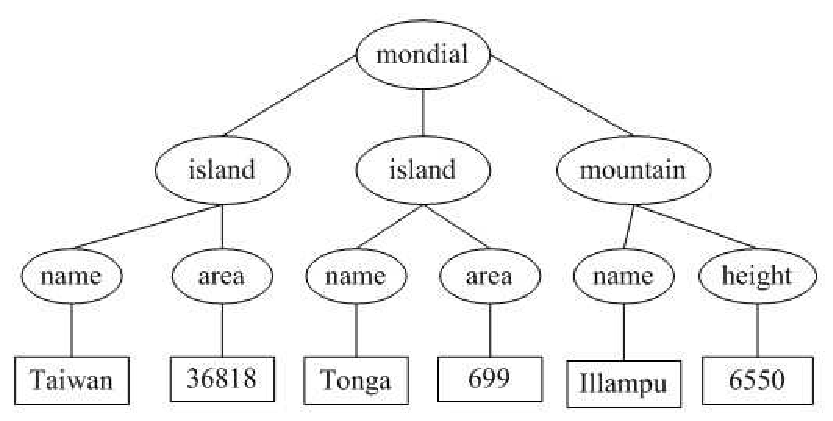
\includegraphics[width=0.4\textwidth]{XML}
\caption{树状结构}\label{fig:xml}
\vspace{\baselineskip}
\end{figure}


其插入图片的代码及其说明如下。
\vspace{1em}\noindent\hrule
\begin{verbatim}
\begin{figure}[htbp]
\centering
\includegraphics[width=0.4\textwidth]{文件名(.eps)}
\caption{标题}\label{标签名(通常为 fig:labelname)}
\vspace{\baselineskip} %表示图与正文空一行
\end{figure}
\end{verbatim}

\noindent\hrule

\begin{verbatim}
figure环境的可选参数[htbp]表示浮动图形所放置的位置,h (here)表示当前位置,t (top)表示页芯顶部,b (bottom)表示页芯底部,p (page)表示单独一页。在Word等软件中,图片通常插入到当前位置,如果当前页的剩余空间不够,图片将被移动到下一页,当前页就会出现很大的空白,其人工调整工作非常不便。由LaTeX提供的浮动图片功能,总是会按h->t->b->p的次序处理选项中的字母,自动调整图片的位置,大大减轻了工作量。
\centering命令将后续内容转换成每行皆居中的格式。
"\includegraphics"的可选参数用来设置图片插入文中的水平宽度,一般表示为正文宽度(\textwidth)的倍数。
\caption命令可选参数“标签名”为英文形式,一般不以图片或表格的数字顺序作为标签,而应包含一定的图片或表格信息,以便于文中引用(若图片、表格、公式、章节和参考文献等在文中出现的先后顺序发生了变化,其标注序号及其文中引用序号也会跟着发生变化,这一点是Word等软件所不能做到的)。另外,图题或表题并不会因为分页而与图片或表格体分置于两页,章节等各级标题也不会置于某页的最底部,LaTeX系统会自动调整它们在正文中的位置,这也是Word等软件所无法匹敌的。
\vspace将产生一定高度的竖直空白,必选参数为负值表示将后续文字位置向上提升,参数值可自行调整。em为长度单位,相当于大写字母M的宽度。\vspace{\baselineskip} 表示图与正文空一行。
引用方法:“见图~\ref{fig:figname}”、“如图~\ref{fig:figname}~所示”等。
\end{verbatim}

\noindent\hrule\vspace{1em}

若需要将~2~张及以上的图片并排插入到一行中,则需要采用\verb|minipage|环境,如图~\ref{fig:dd}~和图~\ref{fig:ds}~所示。
\begin{figure}[htbp]
\centering
\begin{minipage}{0.4\textwidth}
\centering
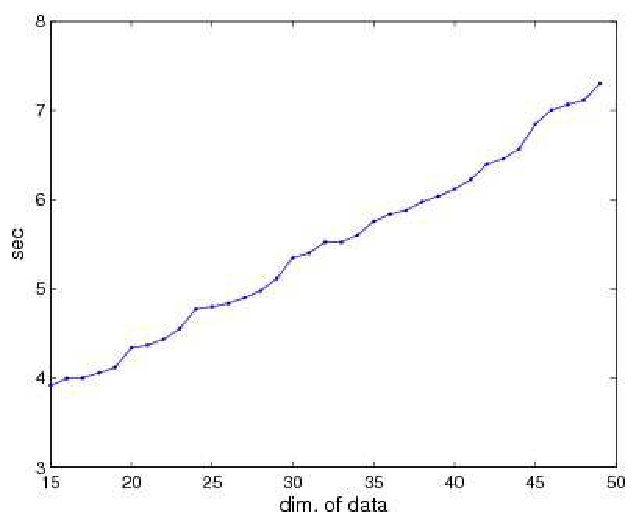
\includegraphics[width=\textwidth]{dataDimensions}
\caption{数据维数的变化}\label{fig:dd}
\end{minipage}
\begin{minipage}{0.4\textwidth}
\centering
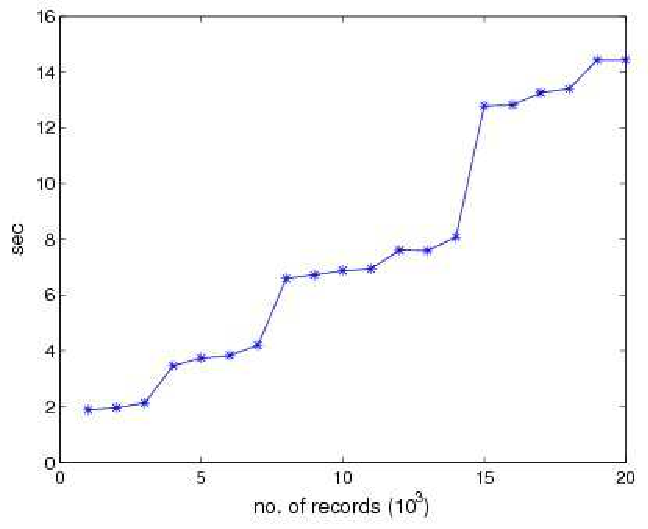
\includegraphics[width=\textwidth]{dataSize}
\caption{数据规模的变化}\label{fig:ds}
\end{minipage}
\vspace{\baselineskip}
\end{figure}

其代码如下所示。
\vspace{1em}\noindent\hrule
\begin{verbatim}
\begin{figure}[htbp]
\centering
\begin{minipage}{0.4\textwidth}
\centering
\includegraphics[width=\textwidth]{文件名}
\caption{标题}\label{fig:f1}
\end{minipage}
\begin{minipage}{0.4\textwidth}
\centering
\includegraphics[width=\textwidth]{文件名}
\caption{标题}\label{fig:f2}
\end{minipage}\vspace{\baselineskip}
\end{figure}
\end{verbatim}

\noindent\hrule

\begin{verbatim}
minipage环境的必选参数用来设置小页的宽度,若需要在一行中插入n个等宽图片,则每个小页的宽度应略小于(1/n)\textwidth。
\end{verbatim}

\noindent\hrule

\section{具有子图的图片插入方法}

图中若含有子图时,需要调用~subfigure~宏包, 如图~\ref{fig:subfig}~所示。
\begin{figure}[htbp]
  \centering
  \subfigure[Data Dimensions]{\label{fig:subfig:datadim}
                \includegraphics[width=0.4\textwidth]{dataDimensions}}
  \subfigure[Data Size]{\label{fig:subfig:datasize}
                \includegraphics[width=0.4\textwidth]{dataSize}}
  \caption{Scalability of data}\label{fig:subfig}
\vspace{\baselineskip}
\end{figure}

其代码及其说明如下。
\vspace{1em}\noindent\hrule

\begin{verbatim}
\begin{figure}[htbp]
  \centering
  \subfigure[第1个子图标题]{
            \label{第1个子图标签(通常为 fig:subfig1:subsubfig1)}
            \includegraphics[width=0.4\textwidth]{文件名}}
  \subfigure[第2个子图标题]{
            \label{第2个子图标签(通常为 fig:subfig1:subsubfig2)}
            \includegraphics[width=0.4\textwidth]{文件名}}
  \caption{总标题}\label{总标签(通常为 fig:subfig1)}
\vspace{\baselineskip}
\end{figure}
\end{verbatim}

\noindent\hrule

\begin{verbatim}
子图的标签实际上可以随意设定,只要不重复就行。但为了更好的可读性,我们建议fig:subfig:subsubfig格式命名,这样我们从标签名就可以知道这是一个子图引用。
引用方法:总图的引用方法同本章第1节,子图的引用方法用\ref{fig:subfig:subsubfig}来代替。
\end{verbatim}

\noindent\hrule\vspace{1em}

子图的引用示例:如图~\ref{fig:subfig:datadim}~和图~\ref{fig:subfig:datasize}~所示。

若想获得插图方法的更多信息,参见网络上的~\href{ftp://ftp.tex.ac.uk/tex-archive/info/epslatex.pdf}{Using Imported Graphics in \LaTeX and pdf\LaTeX}~文档。 

\section{插入算法}

\begin{algorithm}[!h]
{
{
\renewcommand\baselinestretch{1.5}\selectfont %控制行距
\caption{ Scheduling Algorithm }
\label{alg:schedule}
\begin{algorithmic}[1]
\REQUIRE ~\\
A DFG $G=<V,E>$;\\
An allocation $A(G)$ for $G$.
\ENSURE ~\\
A schedule.
    \STATE{.......................}
    \FOR{$i\leftarrow\ 1\ to\ M$}    
        \STATE{.......................}
    \ENDFOR
    \STATE{.......................}
    \STATE{.......................}
    \STATE{.......................}
    \STATE{.......................}
    \STATE{.......................}
    \FOR{$k\leftarrow\ 1\ to\ |V|$}
        \STATE{.......................}
        \STATE{.......................}
        \STATE{.......................}
        \STATE{.......................}
    \IF{$LT_k==j$}
        \IF{there is no idle core in cluster $cl_{loc}$}
            \STATE{.......................}
            \STATE{.......................}
            \STATE{.......................}
            \STATE{.......................}
            \STATE{.......................}
            \STATE{.......................}
        \ELSE
            \STATE{.......................}
            \STATE{.......................}
            \STATE{.......................}
            \STATE{.......................}
            \STATE{.......................}
            \STATE{.......................}
        \ENDIF
    \ENDIF
    \ENDFOR
 

\end{algorithmic}
}
\par}
\end{algorithm}
%% !Mode:: "TeX:UTF-8"

\chapter{表格的绘制方法}
\section{研究生毕业设计论文的绘表规范}

表应有自明性。表格不加左、右边线。表的编排建议采用国际通行的三线表。表内中文书写使用宋体五号字。

每个表格之上均应有表题(由表序和表名组成)。表序一般按章编排,如第~1~章第一个插表的序号为“表~1-1”等。表序与表名之间空两格,
表名使用中文五号字,居中。表名中不允许使用标点符号,表名后不加标点。
表头设计应简单明了,尽量不用斜线。表头中可采用化学,物理量等专业符号。

全表如用同一单位,则将单位符号移至表头右上角,加圆括号\cite{djy}。
表中数据应准确无误,书写清楚。数字空缺的格内加横线“-”(占~2~个数字宽度)。表内文字或数字上、下或左、右相同时,
采用通栏处理方式,不允许用“〃”、“同上”之类的写法。

表内文字使用宋体五号字,垂直居中书写,起行空一格、转行顶格、句末不加标点。
如某个表需要转页接排,在随后的各页上应重复表的编号。编号后加“(续表)”,表题可省略。续表应重复表头。
表格绘制完成之后,与正文空一行。

\section{普通表格的绘制方法}

表格应具有三线表格式,因此需要调用~booktabs~宏包,其标准格式如表~\ref{tab:table1}~所示。

\renewcommand\arraystretch{1.5}%控制行距
\begin{table}[!h]
\caption{基准测试集参数}\label{tab:bench}
\vspace{0.5em}
\centering
\begin{tabular}{l*{1}{C{2cm}}*{1}{L{6.2cm}}}
\toprule
Name         & $n$ & Description\\
\midrule
Random1      & 50  & Random graph generated by TGFF\\
Random2      & 100 & Random graph generated by TGFF\\
Random3      & 150 & Random graph generated by TGFF\\
Random4      & 200 & Random graph generated by TGFF\\
Random5      & 250 & Random graph generated by TGFF\\
Random6      & 300 & Random graph generated by TGFF\\
Random7      & 350 & Random graph generated by TGFF\\
Random8      & 400 & Random graph generated by TGFF\\
Random9      & 450 & Random graph generated by TGFF\\
Random10     & 500 & Random graph generated by TGFF\\
\bottomrule
\end{tabular}
\vspace{\baselineskip}
\end{table}
\renewcommand\arraystretch{1}

其绘制表格的代码及其说明如下。
\vspace{1em}\noindent\hrule

\begin{verbatim}
\begin{table}[htbp]
\caption{表标题}\label{标签名(通常为 tab:tablename)}
\vspace{0.5em}\centering\wuhao
\begin{tabular}{cc...c}
\toprule[1.5pt]
表头第1个格   & 表头第2个格   & ... & 表头第n个格  \\
\midrule[1pt]
表中数据(1,1) & 表中数据(1,2) & ... & 表中数据(1,n)\\
表中数据(2,1) & 表中数据(2,2) & ... & 表中数据(2,n)\\
表中数据(3,1) & 表中数据(3,2) & ... & 表中数据(3,n)\\
表中数据(4,1) & 表中数据(4,2) & ... & 表中数据(4,n)\\
...................................................\\
表中数据(m,1) & 表中数据(m,2) & ... & 表中数据(m,n)\\
\bottomrule[1.5pt]
\end{tabular}
\vspace{\baselineskip}
\end{table}
\end{verbatim}

\noindent\hrule

\begin{verbatim}
table环境是一个将表格嵌入文本的浮动环境。
\wuhao命令将表格的字号设置为五号字(10.5pt),在绘制表格结束退出时,不需要将字号再改回为\xiaosi,正文字号默认为小四号字(12pt)。
tabular环境的必选参数由每列对应一个格式字符所组成:c表示居中,l表示左对齐,r表示右对齐,其总个数应与表的列数相同。此外,@{文本}可以出现在任意两个上述的列格式之间,其中的文本将被插入每一行的同一位置。表格的各行以\\分隔,同一行的各列则以&分隔。
\toprule、\midrule和\bottomrule三个命令是由booktabs宏包提供的,其中\toprule和\bottomrule分别用来绘制表格的第一条(表格最顶部)和第三条(表格最底部)水平线,\midrule用来绘制第二条(表头之下)水平线,且第一条和第三条水平线的线宽为1.5pt,第二条水平线的线宽为1pt。
引用方法:“如表~\ref{tab:tablename}~所示”。
\end{verbatim}

\noindent\hrule

\section{长表格的绘制方法}

长表格是当表格在当前页排不下而需要转页接排的情况下所采用的一种表格环境。若长表格仍按照普通表格的绘制方法来获得,
其所使用的\verb|table|浮动环境无法实现表格的换页接排功能,表格下方过长部分会排在表格第1页的页脚以下。为了能够实现长表格的转页接排功能,
需要调用~longtable~宏包,由于长表格是跨页的文本内容,因此只需要单独的\verb|longtable|环境,所绘制的长表格的格式如表~\ref{tab:table2}~所示。

此长表格~\ref{tab:table2}~第~2~页的标题“编号(续表)”和表头是通过代码自动添加上去的,无需人工添加,若表格在页面中的竖直位置发生了变化,长表格在第~2~页
及之后各页的标题和表头位置能够始终处于各页的最顶部,也无需人工调整,\LaTeX~系统的这一优点是~Word~等软件所无法企及的。

下段内容是为了让下面的长表格分居两页,看到表标题“编号(续表)”的效果。摘录于《你若安好,便是晴天 -- 林徽因传》片段:

她叫林徽因,出生于杭州,是许多人梦中期待的白莲。她在雨雾之都伦敦,发生过一场空前绝后的康桥之恋。她爱过三个男子,爱得清醒,也爱得平静。徐志摩为她徜徉在康桥,深情地等待一场旧梦可以归来。梁思成与她携手走过千山万水,为完成使命而相约白头。金岳霖为她终身不娶,痴心不改地守候一世。可她懂得人生飘忽不定,要学会随遇而安。
真正的平静,不是避开车马喧嚣,而是在心中修篱种菊。尽管如流往事,每一天都涛声依旧,只要我们消除执念,便可寂静安然。愿每个人在纷呈世相中不会迷失荒径,可以端坐磐石上,醉倒落花前。
如果可以,请让我预支一段如莲的时光,哪怕将来某一天加倍偿还。这个雨季会在何时停歇,无从知晓。但我知道,你若安好,便是晴天。					
\wuhao\begin{longtable}{ccc}
\caption{湖南大学各学院名称一览}\label{tab:table2}
 \vspace{0.5em}\\
\toprule[1.5pt] 学院名称 & 网址 & 联系电话  \\ \midrule[1pt]
\endfirsthead
\multicolumn{3}{c}{表~\thetable(续表)}\vspace{0.5em}\\
\toprule[1.5pt] 学院名称 & 网址 & 联系电话  \\ \midrule[1pt]
\endhead
\bottomrule[1.5pt]
\endfoot
机械工程学院& \url{http://tdjxxy.tju.edu.cn/}& 87401979\\
精密仪器与光电子工程学院&  \url{http://www2.tju.edu.cn/colleges/precision/cn/}& 27404775\\
电子信息工程学院& \url{http://www.tju.edu.cn/seie}& 27406956\\
电气与自动化工程学院& \url{http://www2.tju.edu.cn/colleges/automate/}& 27405477\\
建筑工程学院& \url{http://www2.tju.edu.cn/colleges/civil/}& 27404072\\
化工学院& \url{http://chemeng.tju.edu.cn/}& 27403389\\
材料科学与工程学院& \url{http://mse.tju.edu.cn}& 27406693 \\
建筑学院& \url{http://hgw022072.chinaw3.com/}& 27402724-2111\\
求是学部\\
管理与经济学部&	\url{ http://sm.tju.edu.cn}& 27403423\\
理学院& \url{ http://www.tju.edu.cn/science/}& 27404118\\
文法学院& \url{ http://www2.tju.edu.cn/colleges/sociology/new/}& 27403691\\
软件学院& \url{http://scs.tju.edu.cn}& 87401540\\
计算机科学与技术学院& \url{http://cs.tju.edu.cn/}& 27406538\\
马克思主义学院& \url{http://www2.tju.edu.cn/colleges/marxism/}& 27405348\\
环境科学与工程学院& \url{http://www.tju.edu.cn/see}& 87402072\\
药物科学与技术学院& \url{http://www2.tju.edu.cn/colleges/pharmtier/}& 87401830\\
教育学院& \url{http://soe.tju.edu.cn/}& 27401028\\
职业技术教育学院& \url{http://202.113.0.248:8888}\\
继续教育学院& \url{http://aectu.tju.edu.cn/}& 27406298\\
仁爱学院& \url{http://www.tjrac.edu.cn/}& 68579990\\
农业与生物工程学院& \url{http://202.113.13.169/site/nongxueyuan/}& 87402171\\
国际教育学院 & \url{http://www.ietju.com/}& 27406147\\
网络教育学院 & \url{http://www.etju.com/}& 27426952 \\

\end{longtable}\xiaosi
\vspace{\baselineskip}

绘制长表格的代码及其说明如下。
\vspace{1em}\noindent\hrule

\begin{verbatim}
\wuhao\begin{longtable}{cc...c}
\caption{表标题}\label{标签名(通常为 tab:tablename)}\\
\toprule[1.5pt] 表头第1个格 & 表头第2个格 & ... & 表头第n个格\\ \midrule[1pt]
\endfirsthead
\multicolumn{n}{c}{表~\thetable(续表)}\vspace{0.5em}\\
\toprule[1.5pt] 表头第1个格 & 表头第2个格 & ... & 表头第n个格\\ \midrule[1pt]
\endhead
\bottomrule[1.5pt]
\endfoot
表中数据(1,1) & 表中数据(1,2) & ... & 表中数据(1,n)\\
表中数据(2,1) & 表中数据(2,2) & ... & 表中数据(2,n)\\
...................................................\\
表中数据(m,1) & 表中数据(m,2) & ... & 表中数据(m,n)\\
\end{longtable}\xiaosi
\end{verbatim}

\noindent\hrule
\begin{verbatim}
在绘制长表格的前面留出一个空白行,并在第2行的一开始全局定义长表格的字号为五号字,这样能够保证长表格之前段落的行距保持不变。
在绘制长表格结束后,需要\xiaosi命令重新将字号改为小四号字。
\endhead之前的文字描述的是第2页及其之后各页的标题或表头;
\endfirsthead之前的文字描述的是第1页的标题和表头,若无此命令,则第1页的表头和标题由\endhead命令确定;
同理,\endfoot之前的文字描述的是除最后一页之外每页的表格底部内容;
\endlastfoot之前的文字描述的是最后一页的表格底部内容,若无此命令,
则最后一页的表格底部内容由\endfoot命令确定;由于规范中长表格每页底部内容均相同(水平粗线),因此模板中没有用到\endlastfoot命令。
\end{verbatim}

\noindent\hrule
\section{列宽可调表格的绘制方法}
论文中能用到列宽可调表格的情况共有两种:一种是当插入的表格某一单元格内容过长以至于一行放不下的情况,
另一种是当对公式中首次出现的物理量符号进行注释的情况。这两种情况都需要调用~tabularx~宏包。下面将分别对这两种情况下可调表格的绘制方法进行阐述。
\subsection{表格内某单元格内容过长的情况}

首先给出这种情况下的一个例子如表~\ref{tab:table3}~所示。
\begin{table}[htbp]
\caption{最小的三个正整数的英文表示法}\label{tab:table3}
\vspace{0.5em}\wuhao
\begin{tabularx}{\textwidth}{llX}
\toprule[1.5pt]
Value & Name & Alternate names, and names for sets of the given size\\\midrule[1pt]
1 & One & ace, single, singleton, unary, unit, unity\\
2 & Two & binary, brace, couple, couplet, distich, deuce, double, doubleton, duad, duality, duet, duo, dyad, pair, snake eyes, span, twain, twosome, yoke\\
3 & Three & deuce-ace, leash, set, tercet, ternary, ternion, terzetto, threesome, tierce, trey, triad, trine, trinity, trio, triplet, troika, hat-trick\\\bottomrule[1.5pt]
\end{tabularx}
\vspace{\baselineskip}
\end{table}
绘制这种表格的代码及其说明如下。
\vspace{1em}\noindent\hrule
\begin{verbatim}
\begin{table}[htbp]
\caption{表标题}\label{标签名(通常为 tab:tablename)}
\vspace{0.5em}\wuhao
\begin{tabularx}{\textwidth}{l...X...l}
\toprule[1.5pt]
表头第1个格   & ... & 表头第X个格   & ... & 表头第n个格  \\
\midrule[1pt]
表中数据(1,1) & ... & 表中数据(1,X) & ... & 表中数据(1,n)\\
表中数据(2,1) & ... & 表中数据(2,X) & ... & 表中数据(2,n)\\
.........................................................\\
表中数据(m,1) & ... & 表中数据(m,X) & ... & 表中数据(m,n)\\
\bottomrule[1.5pt]
\end{tabularx}
\vspace{\baselineskip}
\end{table}
\end{verbatim}

\noindent\hrule
\begin{verbatim}
tabularx环境共有两个必选参数:第1个参数用来确定表格的总宽度,这里取为排版表格能达到的最大宽度——正文宽度\textwidth;第2个参数用来确定每列格式,其中标为X的项表示该列的宽度可调,其宽度值由表格总宽度确定。
标为X的列一般选为单元格内容过长而无法置于一行的列,这样使得该列内容能够根据表格总宽度自动分行。若列格式中存在不止一个X项,则这些标为X的列的列宽相同,因此,一般不将内容较短的列设为X。
标为X的列均为左对齐,因此其余列一般选为l(左对齐),这样可使得表格美观,但也可以选为c或r。
\end{verbatim}

\noindent\hrule
\subsection{对物理量符号进行注释的情况}
为使得对公式中物理量符号注释的转行与破折号“———”后第一个字对齐,此处最好采用表格环境。此表格无任何线条,左对齐,
且在破折号处对齐,一共有“式中”二字、物理量符号和注释三列,表格的总宽度可选为文本宽度,因此应该采用\verb|tabularx|环境。
由\verb|tabularx|环境生成的对公式中物理量符号进行注释的公式如式(\ref{eq:1})所示。
%\vspace*{10pt}

\begin{equation}\label{eq:1}
\ddot{\boldsymbol{\rho}}-\frac{\mu}{R_{t}^{3}}\left(3\mathbf{R_{t}}\frac{\mathbf{R_{t}\rho}}{R_{t}^{2}}-\boldsymbol{\rho}\right)=\mathbf{a}
\end{equation}

\begin{tabularx}{\textwidth}{@{}l@{\quad}r@{———}X@{}}
式中& $\bm{\rho}$ &追踪飞行器与目标飞行器之间的相对位置矢量;\\
&  $\bm{\ddot{\rho}}$&追踪飞行器与目标飞行器之间的相对加速度;\\
&  $\mathbf{a}$   &推力所产生的加速度;\\
&  $\mathbf{R_t}$ & 目标飞行器在惯性坐标系中的位置矢量;\\
&  $\omega_{t}$ & 目标飞行器的轨道角速度;\\
&  $\mathbf{g}$ & 重力加速度,$=\frac{\mu}{R_{t}^{3}}\left(
3\mathbf{R_{t}}\frac{\mathbf{R_{t}\rho}}{R_{t}^{2}}-\bm{\rho}\right)=\omega_{t}^{2}\frac{R_{t}}{p}\left(
3\mathbf{R_{t}}\frac{\mathbf{R_{t}\rho}}{R_{t}^{2}}-\bm{\rho}\right)$,这里~$p$~是目标飞行器的轨道半通径。
\end{tabularx}
\vspace{\wordsep}

其中生成注释部分的代码及其说明如下。

\vspace{1em}\noindent\hrule

\begin{verbatim}
\begin{tabularx}{\textwidth}{@{}l@{\quad}r@{— — —}X@{}}
式中 & symbol-1 & symbol-1的注释内容;\\
     & symbol-2 & symbol-2的注释内容;\\
     .............................;\\
     & symbol-m & symbol-m的注释内容。
\end{tabularx}\vspace{\wordsep}
\end{verbatim}

\noindent\hrule

\begin{verbatim}
tabularx环境的第1个参数选为正文宽度,第2个参数里面各个符号的意义为:
    第1个@{}表示在“式中”二字左侧不插入任何文本,“式中”二字能够在正文中左对齐,若无此项,则“式中”二字左侧会留出一定的空白;
    @{\quad}表示在“式中”和物理量符号间插入一个空铅宽度的空白;
    @{— — —}实现插入破折号的功能,它由三个1/2的中文破折号构成;
    第2个@{}表示在注释内容靠近正文右边界的地方能够实现右对齐。
\end{verbatim}

\noindent\hrule\vspace{1em}

由此方法生成的注释内容应紧邻待注释公式并置于其下方,因此不能将代码放入\verb|table|浮动环境中。但此方法不能实现自动转页接排,
可能会在当前页剩余空间不够时,全部移动到下一页而导致当前页出现很大空白。因此在需要转页处理时,还请您手动将需要转页的代码放入一个
新的\verb|tabularx|环境中,将原来的一个\verb|tabularx|环境拆分为两个\verb|tabularx|环境。

若想获得绘制表格的更多信息,参见网络上的~\href{http://www.tug.org/pracjourn/2007-1/mori/}{Tables in \LaTeXe: Packages and Methods}~文档。


%% !Mode:: "TeX:UTF-8"

\chapter{数学公式的输入方法}
\section{研究生毕业设计论文的公式规范}

论文中的公式应另起行,原则上应居中书写,与周围文字留有足够的空间区分开。
若公式前有文字(如“解”、“假定”等),文字空两格写,公式仍居中写。公式末不加标点。

公式应标注序号,并将序号置于括号内。 公式序号按章编排,如第~1~章第一个公式序号为“(1-1)”。公式的序号右端对齐。

公式较长时最好在等号“=”处转行,如难实现,则可在~$+$、$-$、$\times$、$\div$~运算符号处转行,转行时运算符号仅书写于转行式前,不重复书写。

文中引用公式时,一般用“见式~(1-1)”或“由公式~(1-1)”。

公式中用斜线表示“除”的关系时应采用括号,以免含糊不清,如~$a/(b\cos x)$。通常“乘”的关系在前,如~$a\cos x/b$而不写成~$(a/b)\cos x$。

不能用文字形式表示等式,如:$\textnormal{刚度}=\frac{{\textnormal{受力}}}{{\textnormal{受力方向的位移}}}$。

对于数学公式的输入方法,网络上有一个比较全面权威的文档\textbf{~\href{http://tug.ctan.org/cgi-bin/ctanPackageInformation.py?id=voss-mathmode}{Math mode}}~请大家事先大概浏览一下。下面将对学位论文中主要用到的数学公式排版形式进行阐述。

\section{生成~\LaTeX~数学公式的两种方法}
对于先前没有接触过~\LaTeX~的人来说,编写~\LaTeX~数学公式是一件很繁琐的事,尤其是对复杂的数学公式来说,更可以说是一件难以完成的任务。
实际上,生成~\LaTeX~数学公式有两种较为简便的方法,一种是基于~MathType~数学公式编辑器的方法,另一种是基于~MATLAB~商业数学软件的方法,
下面将分别对这两种数学公式的生成方法作一下简单介绍。

\subsection{基于~MathType~软件的数学公式生成方法}
MathType~是一款功能强大的数学公式编辑器软件,能够用来在文本环境中插入~Windows OLE~图形格式的复杂数学公式,所以应用比较普遍。但此软件只有~30~天的试用期,之后若再继续使用则需要付费购买才行。网络上有很多破解版的~MathType~软件可供下载免费使用,
笔者推荐下载安装版本号在~6.5~之上的中文破解版。

在安装好~MathType~之后,若在输入窗口中编写数学公式,复制到剪贴板上的仍然是图形格式的对象。
若希望得到可插入到~\LaTeX~编辑器中的文本格式对象,则需要对~MathType~软件做一下简单的设置:在~MathType~最上排的按钮中依次选择“参数选项
$\to$转换”,在弹出的对话窗中选中“转换到其它语言(文字):”,在转换下拉框中选择“Tex~--~--~LaTeX 2.09 and later”,并将对话框最下方的两个复选框全部勾掉,点击确定,这样,再从输入窗口中复制出来的对象就是文本格式的了,就可以直接将其粘贴到~\LaTeX~
编辑器中了。按照这种方法生成的数学公式两端分别有标记\verb|\[|和标记\verb|\]|,在这两个标记之间才是真正的数学公式代码。

若希望从~MathType~输入窗口中复制出来的对象为图形格式,则只需再选中“公示对象(Windows OLE~图形)”即可。

\subsection{基于~MATLAB~软件的数学公式生成方法}

MATLAB~是矩阵实验室(Matrix Laboratory)的简称,是美国~MathWorks~公司出品的商业数学软件。它是当今科研领域最常用的应用软件之一,
具有强大的矩阵计算、符号运算和数据可视化功能,是一种简单易用、可扩展的系统开发环境和平台。

MATLAB~中提供了一个~latex~函数,它可将符号表达式转化为~\LaTeX~数学公式的形式。其语法形式为~latex(s),其中,~s~为符号表达式,
之后再将~latex~函数的运算结果直接粘贴到~\LaTeX~编辑器中。从~\LaTeX~数学公式中可以发现,其中可能包含如下符号组合:

\begin{verbatim*}
\qquad=两个空铅(quad)宽度
\quad=一个空铅宽度
\;=5/18空铅宽度
\:=4/18空铅宽度
\,=3/18空铅宽度
\!=-3/18空铅宽度
\ =一个空格
\end{verbatim*}

所以最好将上述符号组合从数学公式中删除,从而使数学公式显得匀称美观。

对于~Word~等软件的使用者来说,在我们通过~MATLAB~运算得到符号表达式形式的运算结果时,在~Word~中插入运算结果需要借助于~MathType~软件,
通过在~MathType~中输入和~MATLAB~运算结果相对应的数学表达形式,之后再将~MathType~数学表达式转换为图形格式粘贴到~Word~中。实际上,
也可以将~MATLAB~中采用~latex~函数运行的结果直接粘贴到~MathType~中,再继续上述步骤,这样可以大大节省输入公式所需要的时间。
此方法在~MathType~6.5c~上验证通过,若您粘入到~MathType~中的仍然为从~MATLAB~中导入的代码,请您更新~MathType~软件。

\section{数学字体}
在数学模式下,常用的数学字体命令有如下几种:

\begin{verbatim}
\mathnormal或无命令 用数学字体打印文本;
\mathit             用斜体(\itshape)打印文本;
\mathbf             用粗体(\bfseries)打印文本;
\mathrm             用罗马体(\rmfamily)打印文本;
\mathsf             用无衬线字体(\sffamily)打印文本;
\mathtt             用打印机字体(\ttfamily)打印文本;
\mathcal            用书写体打印文本;
\end{verbatim}

在学位论文撰写中,只需要用到上面提到的~\verb|\mathit|、\verb|\mathbf|~和~\verb|\mathrm|~命令。若要得到~Times New Roman~的数学字体,则需要调用~txfonts~宏包(此宏包实际上采用的是~Nimbus Roman No9 L~字体,
它是开源系统中使用的免费字体,其字符字体与~Times New Roman~字体几乎完全相同);若要得到粗体数学字体,则需要调用~bm~宏包。表~\ref{tab:fonts}~中分别列出了得到阿拉伯数字、拉丁字母和希腊字母
各种数学字体的命令。

\begin{table}[htbp]
\caption{常用数学字体命令一览}\label{tab:fonts}
\vspace{0.5em}\centering\wuhao
\begin{tabular}{llll}
\toprule
 & 阿拉伯数字\&大写希腊字母 & 大小写拉丁字母 & 小写希腊字母  \\
\midrule
斜体 & \verb|\mathit{}| & \verb|无命令| & \verb|无命令|\\
粗斜体 & \verb|\bm{\mathit{}}| & \verb|\bm{}| & \verb|\bm{}|\\
直立体 & \verb|无命令| & \verb|\mathrm{}| & \verb|字母后加up|\\
粗体 & \verb|\mathbf{}或\bm{}| & \verb|\mathbf{}| & \verb|\bm{字母后加up}|\\
\bottomrule
\end{tabular}
\vspace{\baselineskip}
\end{table}

\noindent 下面列出了一些应采用直立数学字体的数学常数和数学符号。

\vspace{-0.5em}\begin{center}\begin{tabularx}{0.7\textwidth}{XX}
$\mathrm{d}$、 $\mathrm{D}$、 $\mathrm{p}$~———微分算子 & $\mathrm{e}$~———自然对数之底数\\
$\mathrm{i}$、 $\mathrm{j}$~———虚数单位 & $\piup$———圆周率\\
\end{tabularx}\end{center}

\section{行内公式}
出现在正文一行之内的公式称为行内公式,例如~$f(x)=\int_{a}^{b}\frac{\sin{x}}{x}\mathrm{d}x$。对于非矩阵和非多行形式的行内公式,一般不会使得行距发生变化,而~Word~等软件却会根据行内公式的竖直距离而自动调节行距,如图~\ref{fig:hangju}~所示。

\begin{figure}[htbp]
\centering
\subfigure[由~\LaTeX~系统生成的行内公式]{\label{fig:subfig:latex}
                \fbox{\includegraphics[width=0.55\textwidth]{latex}}}
\subfigure[由~Word软件生成的~.doc~格式行内公式]{\label{fig:subfig:word}
                \fbox{\includegraphics[width=0.55\textwidth]{word}}}
\subfigure[由~Word软件生成的~.pdf~格式行内公式]{\label{fig:subfig:pdf}
                \fbox{\includegraphics[width=0.55\textwidth]{pdf}}}

\caption{由~\LaTeX~和~Word~生成的~3~种行内公式屏显效果}\label{fig:hangju}
\vspace{-1em}
\end{figure}

这三幅图分别为~\LaTeX~和~Word~生成的行内公式屏显效果,从图中可看出,在~\LaTeX~文本含有公式的行内,在正文与公式之间对接工整,行距不变;而在~Word~文本含有公式的行内,在正文与公式之间对接不齐,行距变大。因此从这一点来说,
\LaTeX~系统在数学公式的排版上具有很大优势。

\LaTeX~提供的行内公式最简单、最有效的方法是采用~\TeX~本来的标记———开始和结束标记都写作~\$,例如本段开始的例子可由下面的输入得到。
\verb|$f(x)=\int_{a}^{b}\frac{\sin{x}}{x}\mathrm{d}x$|

\section{行间公式}
位于两行之间的公式称为行间公式,每个公式都是一个单独的段落,例如
\[\int_a^b{f\left(x\right)\mathrm{d}x}=\lim_{\left\|\Delta{x_i}\right\|\to 0}\sum_i{f\left(\xi_i\right)\Delta{x_i}}\]
除人工编号外,\LaTeX~各种类型行间公式的标记见表~\ref{tab:eqtag}。
\begin{table}[htbp]
\caption{各种类型行间公式的标记}\label{tab:eqtag}
\vspace{0.5em}\centering\wuhao
\begin{tabularx}{\textwidth}{cll}
\toprule
& 无编号 & 自动编号\\
\midrule
单行公式& \verb|\begin{displaymath}... \end{displaymath}|& \verb|\begin{equation}... \end{equation}|\\
        & 或~\verb|\[...\]| & \\
多行公式& \verb|\begin{eqnarray*}... \end{eqnarray*}|& \verb|\begin{eqnarray}... \end{eqnarray}|\\
\bottomrule
\end{tabularx}
\end{table}

另外,在自动编号的某行公式行尾添加标签~\verb|\nonumber|,可将该行转换为无编号形式。

行间多行公式需采用~\verb|eqnarray|~或~\verb|eqnarray*|~环境,它默认是一个列格式为~\verb|rcl|~的~3~列矩阵,并且中间列的字号要小一些,因此通常只将需要对齐的运算符号(通常为等号“=”)置于中间列。

\section{可自动调整大小的定界符}
若在左右两个定界符之前分别添加命令~\verb|\left|~和~\verb|\right|,则定界符可根据所包围公式大小自动调整其尺寸,这可从式(\ref{nodelimiter})和式(\ref{delimiter})中看出。
\begin{equation}\label{nodelimiter}
(\sum_{k=\frac12}^{N^2})
\end{equation}
\begin{equation}\label{delimiter}
\left(\sum_{k=\frac12}^{N^2}\right)
\end{equation}
式(\ref{nodelimiter})和式(\ref{delimiter})是在~\LaTeX~中分别输入如下代码得到的。
\begin{verbatim}
(\sum_{k=\frac12}^{N^2})
\left(\sum_{k=\frac12}^{N^2}\right)
\end{verbatim}
\verb|\left|~和~\verb|\right|~总是成对出现的,若只需在公式一侧有可自动调整大小的定界符,则只要用“.”代替另一侧那个无需打印出来的定界符即可。

若想获得关于此部分内容的更多信息,可参见~\href{http://tug.ctan.org/cgi-bin/ctanPackageInformation.py?id=voss-mathmode}{Math mode}~文档的第~8~章“Brackets, braces and parentheses”。

\section{数学重音符号}
数学重音符号通常用来区分同一字母表示的不同变量,输入方法如下(需要调用~\verb|amsmath|~宏包):

\vspace{0.5em}\noindent\wuhao\begin{tabularx}{\textwidth}{Xc|Xc|Xc}
 \verb|\acute| & $\acute{a}$ & \verb|\mathring| & $\mathring{a}$ & \verb|\underbrace| & $\underbrace{a}$ \\
 \verb|\bar| & $\bar{a}$ & \verb|\overbrace| & $\overbrace{a}$ & \verb|\underleftarrow| & $\underleftarrow{a}$ \\
 \verb|\breve| & $\breve{a}$ & \verb|\overleftarrow| & $\overleftarrow{a}$ & \verb|\underleftrightarrow| & $\underleftrightarrow{a}$ \\
 \verb|\check| & $\check{a}$ & \verb|\overleftrightarrow| & $\overleftrightarrow{a}$ & \verb|\underline| & $\underline{a}$ \\
 \verb|\dddot| & $\dddot{a}$ & \verb|\overline| & $\overline{a}$ & \verb|\underrightarrow| & $\underrightarrow{a}$ \\
 \verb|\ddot| & $\ddot{a}$ & \verb|\overrightarrow| & $\overrightarrow{a}$ & \verb|\vec| & $\vec{a}$ \\
 \verb|\dot| & $\dot{a}$ & \verb|\tilde| & $\tilde{a}$ & \verb|\widehat| & $\widehat{a}$ \\
 \verb|\grave| & $\grave{a}$ & \verb|\underbar| & $\underbar{a}$ & \verb|\widetilde| & $\widetilde{a}$ \\
 \verb|\hat| & $\hat{a}$
\end{tabularx}\vspace{0.5em}
\xiaosi 当需要在字母~$i$~和~$j$~的上方添加重音符号时,为了去掉这两个字母顶上的小点,这两个字母应该分别改用~\verb|\imath|~和~\verb|\jmath|。

如果遇到某些符号不知道该采用什么命令能输出它时,则可通过~\href{http://detexify.kirelabs.org/classify.html}{Detexify$^2$~网站}来获取符号命令。若用鼠标左键在此网页的方框区域内画出你所要找的符号形状,则会在网页右方列出和你所画符号形状相近的~5~个符号及其相对应的~\LaTeX~输入命令。若所列出的符号中不包括你所要找的符号,还可通过点击“Select from the complete list!”的链接以得分从低到高的顺序列出所有符号及其相对应的~\LaTeX~输入命令。

最后,建议大家还以~\href{http://tug.ctan.org/cgi-bin/ctanPackageInformation.py?id=voss-mathmode}{Math mode}~这篇~pdf~文档作为主要参考。若要获得最为标准、美观的数学公式排版形式,可以查查文档中是否有和你所要的排版形式相同或相近的代码段,通过修改代码段以获得你所要的数学公式排版形式。


%% !Mode:: "TeX:UTF-8"

\chapter{罗列和定理环境使用方法}

\section{单层罗列环境}
湖南大学学位论文一般可采用两种罗列环境:一种是并列条目有同样标签的~\verb|itemize|~罗列环境,另一种是具有自动排序编号符号的~\verb|enumerate|~罗列环境。这两种罗列环境的样式参数可参考图~\ref{fig:list}。
\begin{figure}[htbp]
\centering
\includegraphics[width = 0.6\textwidth]{list}
\caption{罗列环境参数示意图}\label{fig:list}\vspace{-1em}
\end{figure}

通过调用~enumitem~宏包可以很方便地控制罗列环境的布局,其~format.tex~文件中的~\verb|\setitemize|~和~\verb|\setenumerate|~命令分别用来设置~\verb|itemize|~和~\verb|enumerate|~环境的样式参数。采用~\verb|itemize|~单层罗列环境的排版形式如下:

\begin{itemize}
\item 第一个条目文本内容
\item 第二个条目文本内容
\item 第三个条目文本内容
\end{itemize}

其代码如下

\begin{verbatim}
\begin{itemize}
  \item 第一个条目文本内容
  \item 第二个条目文本内容
  ...
  \item 第三个条目文本内容
\end{itemize}
\end{verbatim}

采用~\verb|enumerate|~单层罗列环境的排版形式如下:

\begin{enumerate}
\item 第一个条目文本内容
\item 第二个条目文本内容
\item 第三个条目文本内容
\end{enumerate}

其代码如下

\begin{verbatim}
\begin{enumerate}
  \item 第一个条目文本内容
  \item 第二个条目文本内容
  ...
  \item 第三个条目文本内容
\end{enumerate}
\end{verbatim}



\section{定理环境}

\begin{definition}[谱半径]\label{def:def1}
  称~$n$~阶方阵~$\mathbf{A}$~的全体特征值~$\lambda_1,\cdots,\lambda_n$~组成的集合为~$\mathbf{A}$~的谱,称
  $$\rho(\mathbf{A})=\max{\{|\lambda_1|,\cdots,|\lambda_n|\}}$$
\end{definition}
\begin{theorem}[相似充要条件]\label{lemma:l1}
  方阵$A$和$B$相似的充要条件是:~$A$~和~$B$~有全同的不变因子。
\end{theorem}
\begin{corollary}[推论1]\label{cor:cor1}
在赋范空间~$(X,\|\cdot\|)$~上定义~$d(x,y)=\|x-y\|$, 对任意~$x,y\in X$,~则~$(X,d)$~是距离空间。
\end{corollary}
\begin{proof}
  只需证明~$d(x,y)$~是距离。
\end{proof}
\newpage

定义代码如下:
\begin{verbatim}
 \begin{definition}[谱半径]\label{def:def1}
  称~$n$~阶方阵~$\mathbf{A}$~的全体特征值
  $\lambda_1,\cdots,\lambda_n$组成的集合为~$\mathbf{A}$~的谱,称
  $$\rho(\mathbf{A})=\max{\{|\lambda_1|,\cdots,|\lambda_n|\}}$$
\end{definition}
\end{verbatim}
\noindent\hrule

\vspace{0.1em}\noindent\hrule
\vspace{1em}
定理代码如下:
\begin{verbatim}
\begin{theorem}[相似充要条件]\label{lemma:l1}
  方阵$A$和$B$相似的充要条件是:$A$和$B$有全同的不变因子。
\end{theorem}
\end{verbatim}
\noindent\hrule\vspace{0.1em}

\noindent\hrule
\vspace{1em}
推论和证明代码如下:
\begin{verbatim}
\begin{corollary}[推论1]\label{cor:cor1}
在赋范空间~$(X,\|\cdot\|)$~上定义$d(x,y)=\|x-y\|$,
对任意$x,y\in X$,则$(X,d)$是距离空间。
\end{corollary}
\begin{proof}
  只需证明$d(x,y)$是距离。
\end{proof}
\end{verbatim}
\noindent\hrule\vspace{1em}

定理定义[]中是可选参数,用来说明定理的名称。其他环境格式书写与上面定理、定义、推论格式相同,可自己调用其他环境。
若需要书写定理定义等内容,而且带有顺序编号,需要采用如下环境。除了~\verb|proof|~环境之外,其余~9~个环境都可以有一个可选参数作为附加标题。

\begin{center}
\vspace{0.5em}\noindent\wuhao\begin{tabularx}{0.7\textwidth}{lX|lX}
定理 & \verb|theorem|~环境 & 定义 & \verb|definition|~环境 \\
例 & \verb|example|~环境 & 算法 & \verb|algorithm|~环境 \\
公理 & \verb|axiom|~环境 & 命题 & \verb|proposition|~环境 \\
引理 & \verb|lemma|~环境 & 推论 & \verb|corollary|~环境 \\
注解 & \verb|remark|~环境 & 证明 & \verb|proof|~环境 \\
\end{tabularx}
\end{center} 
\section{conclusion}
\label{sec:conclusion}
%\del{In this paper, we have proved the Min-Min  SRLG-Disjoint routing problem is NP-complete.}
In this paper, we propose an efficient algorithm to solve the Min-Min  SRLG-Disjoint routing problem in the presence of the trap problem. To reduce the complexity of searching for the alternative pair, we propose a divide-and-conquer solution to partition the original Min-Min SRLG-Disjoint routing problem into multiple sub-problems based on a SRLG conflicting link set derived from the AP path encountering the trap problem. Our algorithm takes advantage of existing AP search results and parallel executions for significantly faster path finding.
We have conducted extensive simulations  using the topology trace  on a multi-core CPU platform. The simulation results demonstrate that our algorithm can outperform other approaches with higher routing performance while at a much higher search speed.

%%%%%%%%%% 正文部分内容  %%%%%%%%%%

%%%%%%%%%%  参考文献  %%%%%%%%%%
\defaultfont
\bibliographystyle{HNUThesis}
\phantomsection
\addcontentsline{toc}{chapter}{参考文献}          % 参考文献加入到中文目录
%\nocite{*}                                        % 若将此命令屏蔽掉,则未引用的文献不会出现在文后的参考文献中。
\bibliography{reference}
% !Mode:: "TeX:UTF-8"
\addcontentsline{toc}{chapter}{致\quad 谢} %添加到目录中
\chapter*{致\quad 谢}
本论文的工作是在我的导师[XXXX...] 教授的悉心指导下完成的,[XXXX...]

教授严谨的治学态度和科学的工作方法给了我极大的帮助和影响。在此衷心感谢三年来[XXXX...] 老师对我的关心和指导。

[XXXX...] 教授悉心指导我们完成了实验室的科研工作,在学习上和生活上都给予了我很大的关心和帮助,在此向[XXXX...] 老师表示衷心的谢意。

[XXXX...] 教授对于我的科研工作和论文都提出了许多的宝贵意见,在此表示衷心的感谢。

在实验室工作及撰写论文期间,[XXXX...] 、[XXXX...] 等同学对我论文中的[XXXX...] 研究工作给予了热情帮助,在此向他们表达我的感激之情。

另外也感谢家人[XXXX...] ,他们的理解和支持使我能够在学校专心完成我的学业。



               % 致谢
% !Mode:: "TeX:UTF-8"

\addcontentsline{toc}{chapter}{附录A  发表论文和参加科研情况说明}
\chapter*{附录A~~~~发表论文和参加科研情况说明}
\setlength{\parindent}{0em}
\textbf{(一)发表的学术论文}
\begin{publist}
\item Kun Xie, Heng Tao, Xin Wang, Gaogang Xie, Jigang Wen, Jiannong Cao, Zheng Qin. Divide And Conquer For Fast SRLG Disjoint Routing[C]. DSN 2018: International Conference on Dependable Systems and Networks, Luxerbourg(CCF B).
%\item **. Divide And Conquer For Fast SRLG Disjoint Routing[C]. DSN 2018: International Conference on Dependable Systems and Networks, Luxerbourg(CCF B).
%\item Kun Xie, Heng Tao, Xin Wang, Gaogang Xie, Jigang Wen, Jiannong Cao. Survivable embedded Virtual Network Design to Survive a Substrate Node Failure. (拟投稿)
    %Communication Systems, Networks and Applications, Hongkong, 2010: 325-328. (EI DOI: 10.1109/ICCSNA.2010.5588732)
\end{publist}

\vspace*{1em}
\textbf{(二)申请及已获得的专利}
\begin{publist}
\item 陶恒,谢鲲. 一种求完全风险共享链路组分离路径对的方法及系统:中国。已具有国家知识产权局公开号,并已进入实审阶段。
%1234567.8[P]. 2017-04-25.
%\item **. 一种求完全风险共享链路组分离路径对的方法及系统:中国。%1234567.8[P]. 2017-04-25.
\end{publist}
%\vspace*{1em}
%\textbf{(三)参与的科研项目}
%\begin{publist}
%\item	XXX,XXX. XX~信息管理与信息系统, ~国家自然科学基金项目.课题编号:XXXX.
%\end{publist}
\vfill
\hangafter=1\hangindent=2em\noindent

\setlength{\parindent}{2em}
                   % 发表论文和参加科研情况说明
\clearpage
\end{CJK*}                                        % 结束中文字体使用
\end{document}                                    % 结束全文

%编程语言的基石——Lambda calculus
%http://liujiacai.net/blog/2014/10/12/lambda-calculus-introduction/
